\documentclass[10pt,final]{report}
\usepackage{fontspec}
\usepackage{color}
\usepackage{graphicx}
\DeclareGraphicsExtensions{.png,.pdf,.jpg,.jpeg}
\usepackage{subcaption}
%%% The next two are necessary to get the degree symbol in text and math mode
\usepackage{textcomp}
\usepackage{gensymb}
\usepackage{hyperref}
\hypersetup{%
  colorlinks = true,
  linkcolor  = black,
  urlcolor   = cyan,
  plainpages = false,
  pdfencoding = auto
}
\usepackage{siunitx}
\sisetup{
	range-phrase = -,
	range-units = single
}
% for chemical symbols, relevant for gas mixes, for example
\usepackage[version=4]{mhchem}
\usepackage{hepnames}
%\SetMathAlphabet{\mathup}{bold}{OT1}{\familydefault}{bx}{n}

\usepackage[mathrm=sym, mathup=sym, mathit=sym, mathsf=sym, mathbf=sym, mathtt=sym]{unicode-math}
\defaultfontfeatures{Scale=MatchLowercase}
\setmainfont{Linux Libertine O}
\setsansfont{TeX Gyre Heros}
\setmathfont{TeX Gyre Termes Math}
\usepackage{pdfpages}
\usepackage{tabularx}
\usepackage{booktabs}
\usepackage{pdflscape}
\usepackage{multirow}
\usepackage{adjustbox}
\usepackage{geometry}
\usepackage[backend=biber,sorting=none]{biblatex}
\usepackage{xspace}

\addbibresource{detectorRnD.bib}
\DeclareBibliographyDriver{caliceanalysisnote}{%
    \printnames{author}%
    \newunit\newblock
    \printfield{title}%
    \newunit\newblock
    \printfield{url}%
    \finentry%
}

\DeclareBibliographyDriver{eudetmemo}{%
    \printnames{author}%
    \newunit\newblock
    \printfield{title}%
    \newunit\newblock
    \printfield{url}%
    \finentry%
}

\DeclareBibliographyDriver{eudetreport}{%
    \printnames{author}%
    \newunit\newblock
    \printfield{title}%
    \newunit\newblock
    \printfield{url}%
    \finentry%
}

\DeclareBibliographyDriver{presentation}{%
    \printnames{author}%
    \newunit\newblock
    \printfield{title}%
    \newunit\newblock
    \printfield{conference}%
    \newunit\newblock
    \printfield{location}%
    \newunit\newblock
    \printfield{year}%
    \newunit\newblock
    \printfield{url}%
    \finentry%
}

\begin{document}


\begin{titlepage} 
    \newcommand{\HRule}{\rule{\linewidth}{0.5mm}} % Defines a new command for horizontal lines, change thickness here
	\center % Centre everything on the page
	
	%------------------------------------------------
	%	Headings
	%------------------------------------------------
	
	\textsc{\LARGE Linear Collider Collaboration}\\[1.5cm] % Main heading such as the name of your university/college
		
%	\textsc{\large Minor Heading}\\[0.5cm] % Minor heading such as course title
	
	%------------------------------------------------
	%	Title
	%------------------------------------------------
	
	\HRule\\[0.4cm]
	
	{\huge\bfseries Detector R\&D Report}\\[0.4cm] % Title of your document
	
	\HRule\\[1.5cm]

	% FIXME For the final version, make the version number large again and remove "Draft" and the deadline
	{\Large \color{red}Deadline for submissions: May 15th, 2020}\\
	{\Large DRAFT}\\
    % \textsc{\Large Version 2020.1}\\[0.5cm] % Major heading such as course name
    \textsc{Version 2020.1}\\[0.5cm] % Major heading such as course name

	%------------------------------------------------
	%	Editors
	%------------------------------------------------
	\vfill\vfill
	{\large Editors\\}
	\begin{minipage}[t]{0.49\textwidth}
		\begin{flushleft}
			\large
			\textit{Detector R\&D Liaison}\\
			Maxim \textsc{Titov} \\
			Institut de Recherche sur les lois Fondamentales de l'Univers (IRFU) \\
			CEA - Saclay, F-91191 Gif-sur-Yvette Cedex, France\\
			maxim.titov@cea.fr
		\end{flushleft}
	\end{minipage}\hfill
	\begin{minipage}[t]{0.49\textwidth}
		\begin{flushright}
			\large
			\textit{Detector R\&D Liaison}\\
			Jan F \textsc{Strube} \\
			Pacific Northwest National Laboratory \\
			902 Battelle Boulevard \\
			Richland, WA 99352, USA \\
		\end{flushright}
			\begin{flushright}
				\large
			University of Oregon \\
			Center for High Energy Physics \\
			Eugene, OR 97403, USA \\
			jstrube@uoregon.edu
			\end{flushright}
	\end{minipage}
		
	%------------------------------------------------
	%	Date
	%------------------------------------------------
	\vfill\vfill\vfill % Position the date 3/4 down the remaining page
	{\large\today} % Date, change the \today to a set date if you want to be precise
	
	%------------------------------------------------
	%	Logo
	%------------------------------------------------
	
	\vfill\vfill
    
\includegraphics[width=0.4\textwidth]{signature_red2-cmyk}\\[1cm] % Include a department/university logo
    %
\includegraphics[width=0.15\textwidth]{logo_red2-cmyk}\\[1cm] % Include a department/university logo 
    %
\includegraphics[width=0.2\textwidth]{logotype_red2-cmyk}\\[1cm] % Include a department/university logo 	 
	%----------------------------------------------------------------------------------------
	
	\vfill % Push the date up 1/4 of the remaining page
	
\end{titlepage}

\tableofcontents
\chapter*{Foreword}
\section*{Linear Collider Detector R\&D Liaison Charge}
The LC Detector R\&D Liaisons ensure productive communication between the Linear Collider Collaboration (LCC) Physics and Detectors Executive Board and the detector R\&D groups. The liaisons are in contact with all individual detector R\&D groups relevant to linear colliders to keep track of the overall detector R\&D activities conducted or planned for linear colliders and to periodically compile summaries of the efforts.

\section*{Introduction}
Future accelerator facilities are an indispensable step towards precision determination of the Standard Model parameters, constraining potential new physics contributions or, alternatively, precision studies of New Physics, pending a hint of new physics at other experiments. The quest for the discovery of the Higgs boson with the multipurpose ATLAS and CMS detectors at the LHC imposed major detector instrumentation work, and brought most of the technologies to their performance limits. With many fundamental physics questions within experimental reach (e.g., precision studies of the Higgs boson couplings and other new particles discovered at the LHC) at future accelerator facilities, a large R\&D effort is needed to develop new and advanced innovative concepts for radiation detection.

The physics potential of future accelerators like the ILC or CLIC represents a tremendous challenge for the performance of the detectors, which is in most cases orthogonal to the main directions of development focused on the LHC experiments. Rather than emphasizing radiation hardness and rate capability, the demands for resolution (granularity) and material budget on one hand, and an acceptable speed and power consumption on the other hand, exceed significantly what is now state-of-the-art. Large tracking detectors aim at a 10-fold precision improvement, while simultaneously pushing the limits of sensor and electronics integration and lightweight precision mechanics. The particle flow approach to calorimetry drives the design of highly compact and granular devices with a channel density more than 2 orders of magnitude above the most finely segmented LHC detectors. Such leaps in performance cannot be achieved by a simple extrapolation of the known, but only by entering new technological territory in detector R\&D. Several new concepts for silicon sensor integration, such as monolithic devices, are being pursued for pixel tracking, new micro-pattern gas amplification techniques are explored for use in time projection chambers, and particle flow calorimetry, relying on several novel technologies, promises to deliver unprecedented jet energy resolution, to quote just some examples.

Over the past few decades, extensive generic R\&D studies, applicable to any Linear Collider (LC) detector concept, such as ILD, SiD or CLICdp, have been pursued by the concept-independent R\&D groups and within large collaborations like CALICE, LCTPC and FCAL. This report provides an overview of the past and presently ongoing detector R\&D efforts, including those not directly included in the concept groups today, but which might become relevant in the future. The main purpose if this document is to summarize the LC R\&D achievements worldwide, followed by a discussion of future milestones, in the belief that improved communications will lead to enhancements in the R\&D programs, with a goal to:
\begin{itemize}
\item “Publicize” the technology and provide an update of recent R\&D efforts since the two important milestone documents for each of the projects: the Conceptual Design Report (CDR) for CLIC and the Detailed Baseline Design (DBD) for the ILC;
\item Provide a “snapshot” for a particular technology, without information about manpower needs and financial resources to reach project milestones. As most detector R\&D groups are highly independent with their own funds, this document is not intended to serve as a guideline to control or coordinate different R\&D efforts, by indicating explicitly potential overlap areas;
\item Provide an entry point for new groups in order to help them to learn about the current landscape of the LC R\&D efforts and the areas where they might be interested to contribute.
\end{itemize}
Every individual group was requested to submit a written report describing five items of their R\&D program, as an input to the LC Detector R\&D Liaison report. Suggested content of these documents is approximately as follows:
\begin{itemize}
\item Introduction. Brief overview of the technology (past R\&D efforts with references);
\item Recent milestones since ILC DBD and CLIC CDR to avoid description of historical data;
\item Engineering challenges for a given detector technology in order to encourage new groups to contribute to the engineering aspects and not only to the generic R\&D;
\item Future plans in the years to come and the list of collaborating institutes contributing to the given R\&D technology;
\item Application of the R\&D outside of ILC with references, if technology is already used.
\end{itemize}
The LC Detector R\&D Liaison report serves as an online documentation, updated on a regular basis, and is available to general public and newcomers. The most recent version can be downloaded from: \url{http://linearcollider.web.cern.ch/physics-detectors/working-group-detector-rd-liaison}. This report is not meant to be considered as the summary to select between technologies or advertise the most advanced ones, but rather as a general overview of the landscape of different LC R\&D activities. 

The most recent version 2018.3 (released December 17, 2018) was submitted as supplemental information for the LCC input to the European Strategy update: \url{https://ilchome.web.cern.ch/content/ilc-european-strategy-document}. The next update is planned for June 30, 2020.


\chapter{Vertex Detectors}
\section{Motivation and Constraints for Vertex Detectors at Linear Colliders}

The reconstruction of displaced decays has been an important part of particle physics programs since the days of bubble chambers and the discovery of ``V'' particles. This is still true in today's high-energy collider experiments. If long-lived particles, such as B or D mesons, or tau leptons, decay to at least one charged track in the detector, they can in principle be resolved from the interactions of the primary collision. Similarly, the possibility to distinguish several primary interaction points significantly improves the reconstruction of events. To this end, modern vertex detectors use silicon sensors with small pixels, assembled in support structures with as little material as possible to reduce multiple scattering. A driver for Linear Collider vertex detector R\&D has been low power operation to reduce or completely avoid the need for active cooling.

The reconstruction of displaced vertices depends crucially on the resolution of the perigee, or \emph{impact parameter} of a helical track from the interaction point, which can be parameterized as $\sigma_\text{ip} = \left(\frac{\alpha}{p^{3/2}\sin\theta}\right).$
The goal for the impact parameter resolution in an ILC experiment is $\approx\SI{3}{\micro\meter}$. This puts stringent requirements on the pixel size and the distance of the innermost layer from the interaction point.

Machine-induced background processes at the ILC and CLIC include electron--positron pairs produced in beam--beam interactions. During collisions, vertex detectors accumulate hits from these processes, in addition to those from the primary physics events. In addition to small feature size and low power, it is the reduction of these backgrounds that drives the R\&D for linear collider vertex detectors. Because of the close proximity to the beams, their design is heavily influenced by the beam structure of the accelerator.

In addition to the precise determination of decay vertices, the CLICdp detector and the SiD concept have integrated vertex detectors into their all-silicon tracking systems. This puts additional emphasis on high reliability and high hit detection efficiency.

Highly performing vertex detectors are essential for the success of the physics program at the Linear Collider. Discovery channels for a large class of new physics models involve third-generation fermions: b quarks that form long-lived mesons, top quarks that decay predominantly to a b quark and a W boson, and long-lived tau leptons.

\section{CMOS}
Most recent update: 2020-04-25 \\
Contact person: Marc Winter (email: marc.winter@iphc.cnrs.fr)

\subsection{Introduction}
CMOS Pixel Sensors (CPS) combine high granularity with low material
budget and allow integrating the full signal processing circuitry on
the sensor substrate. They benefit from a steady technological progress 
driven by an industrial market which makes them simultaneously cost 
effective and attractive for a wide range of applications. They are 
developed for an ILC vertex detector since about two decades and were 
shown to rather easily comply with the required spatial resolution 
and material budget expressed in the DBD~\cite{Behnke:2013lya}. The
associated read-out time of a few tens of microseconds represented the
limit achievable with a rolling shutter read-out and the \SI{350}{\nano\meter} CMOS 
technology available at that time. The required radiation tolerance, 
on the other hand, was observed to be well within the sensor potential.
 
The relevance of the technology for subatomic physics experiments is established today with the 400 ULTIMATE sensors operated in the STAR-PXL 
detector~\cite{CONTIN201860} at RHIC/BNL from 2014 to 2016, while the
state of the art is well illustrated by the $\sim$ 20 times faster ALPIDE sensors fabricated ($>$ 20,000 dies) in a \SI{180}{\nano\meter} CMOS technology, to 
equip the upgraded, $>$ \SI{10}{\meter\squared} large, ALICE Inner Tracker System 
(ITS)~\cite{AGLIERIRINELLA2017583}. 
The variety of devices where ULTIMATE has been implemented and, even 
more so, where ALPIDE is foreseen to be integrated, reflects the maturity 
of the technology and the steadily growing interest it generates in the
field.
 
  The detection performances achieved at the time of the DBD 
assumed that integrating the beam related background over several tens 
of bunch-crossings would result in a well affordable disturbance of the 
event reconstruction. Since then, 
potential benefits from shorter integration times, allowing for bunch 
tagging or nearly so, have become clearer and desirable. This applies 
for instance to the distinction between soft tracks due to beamstrahlung
or two-photon collisions and those originating from a displaced vertex
and therefore contributing to the vertex charge. The latter may get  
particularly complicated to reconstruct in case of a higher machine 
luminosity than foreseen in the TDR and of worse running conditions 
than anticipated. 
  
  However, the goal of suppressing the impact of beam related background 
on the physics performance by improving the sensor time resolution to 
$\lesssim$ \SI{1}{\micro\second} steps up the preexisting tension between the 
small pixel size imposed by the required spatial resolution and the 
minimal space needed to implement the very front end circuitry inside 
the pixels. The R\&D pursued so far did not show that a spatial 
resolution of $\lesssim$ \SI{3}{\micro\meter} and a single bunch tagging are 
actually achievable simultaneously within the same, \SI{50}{\micro\meter} thin, 
sensor with the presently available CMOS technologies, moreover with 
a power consumption compatible with air cooling. On the other hand, 
$\sim$ \SI{4}{\micro\meter} spatial resolution may be within reach with sensors 
featuring a continuous read-out time of $\lesssim$ \SI{1}{\micro\second} at an 
affordable power consumption.

  Indirect approaches are therefore being considered to achieve the 
targeted spatial and time resolutions per layer even if they cannot be
reached within a single sensor. They rely on the concept of double-sided detector layers, which provides two hits, one per layer face, for each traversing charged particle. The track 
position and timing are extracted from the combination of the two 
signals delivered by sensors facing each other in the same layer. 
The position and timing may, for instance, come from a high precision 
sensor located on one layer side and a faster, less precise, sensor 
located on the opposite side. Alternatively, the spatial resolution 
may be derived from the combination of opposite, identical, sensors 
limited to \SI{4}{\micro\meter} spatial resolution measurements but providing 
both $\lesssim$ \SI{1}{\micro\second} read-out time.     

\begin{figure}
	\centering
	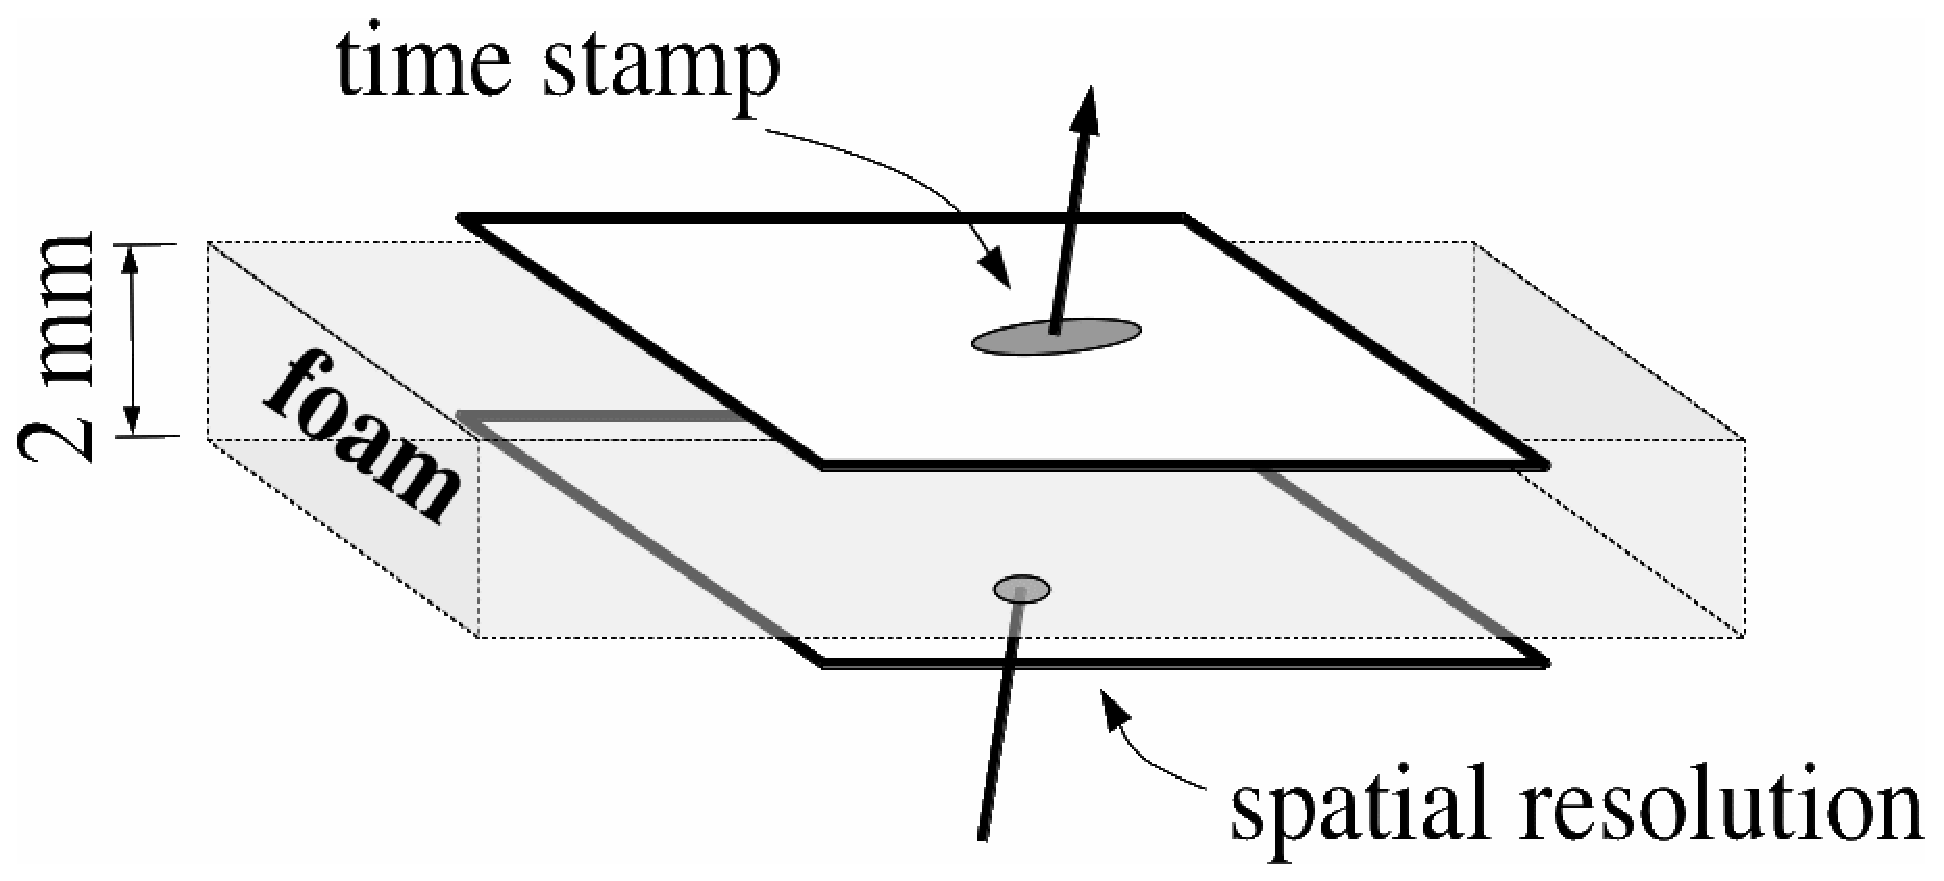
\includegraphics[width=.43\linewidth]{VertexDetector/CMOS/principe-MixedLayers-noPixels.eps}
	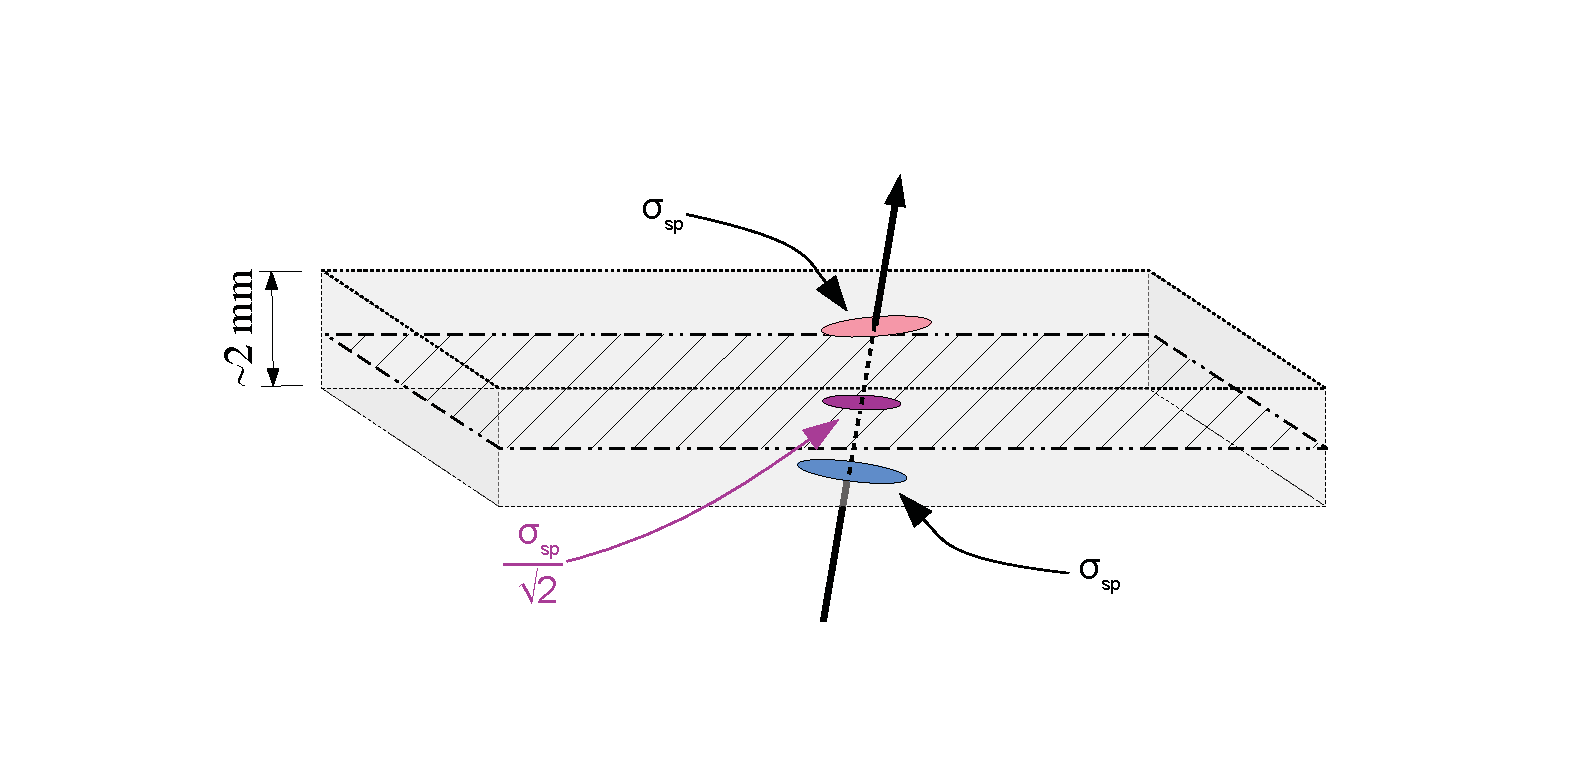
\includegraphics[width=.55\linewidth]{VertexDetector/CMOS/principe-MixedLayers-intermediatePoint.pdf}
	\caption{Alternative approaches based on double-sided layers. Left: particles traverse a "pointing" sensor and a ``timing'' sensor equipping the two faces of a layer. Right: the signals of two ``timing'' sensors featuring $\sim$ \SI{4}{\micro\meter} resolution are combined into a single signal to obtain the required spatial resolution of $\lesssim$ \SI{3}{\micro\meter}.}
	\label{fig:VertexDetector:CMOS:minivectors}
\end{figure}

\subsection{Recent Milestones}
The most advanced CPS under development extendable to bridge the 
gap between ALPIDE and a sensor adapted to an ILC vertex detector 
is the MIMOSIS sensor~\cite{Morel:mimosis}, which is foreseen to 
equip the 4 double-sided stations of the MicroVertex Detector (MVD) 
of the CBM heavy ion experiment at FAIR/GSI. The sensor acts 
simultaneously as a forerunner of a sensor suited to an ILC vertex 
detector. With a pixel array continuous read-out derived from ALPIDE, 
MIMOSIS features a 50 times higher hit density treatment capability 
and a \SI{5}{\micro\second} read-out time. The latter may be compressed to 
$\sim$ \SI{2}{\micro\second} for an ILC vertex detector, with an instantaneous 
power density in the order of $\sim$ SI{50 -- 150}{\mili\watt\per\centimeter\squared}, depending 
on the beam background induced hit density, and thereby on the 
distance to the interaction point. Such performances should allow 
facing the most pessimistic predictions for the background rate 
impinging the vertex detector innermost layer. 

The sensor single point resolution however, is not expected to reach
values well below the ALPIDE value of \SI{5}{\micro\meter} because of the pixel 
footprint imposed by the required in-pixel circuitry, which involves 
about 200 transistors. Optimizing the spatial resolution will consist 
in enhancing charge sharing by using the most appropriate epitaxial 
layer thickness and by tuning the depletion voltage and the steering 
parameters of the in-pixel circuitry. 

After a first prototyping step validating the in-pixel circuitry and the 
pixel array read-out (prototype MIMOSIS-0 featuring $64 \times 504$ pixels), 
the first full scale prototype of MIMOSIS has been fabricated. It 
incorporates $1024 \times 504$ pixels of $\SI{27}{\micro\meter} \times \SI{30}{\micro\meter}$. Its manufacturing 
was accompanied by numerous small prototypes exploring in-pixel circuitry alternatives, allowing in particular for shorter read-out time. They 
are supposed to complement studies made with MIMOSIS-0 showing that the 
sensor charge collection system and the very front-end circuitry are 
suited read-out times shorter than \SI{1}{\micro\second}~\cite{DEVEAUX2020162653}. 
The performance assessment of the complete read-out chain should come 
out through year 2021. Besides the vertex detector, this R\&D also 
applies to tracking subsystems in general. An emblematic example is 
the ILD-SIT, which may be equipped with double-sided layers based on 
$\gtrsim$ \SI{5}{\micro\meter} resolution CPS featuring \SI{1}{\micro\second} read-out time.

 \begin{figure}
	\centering
	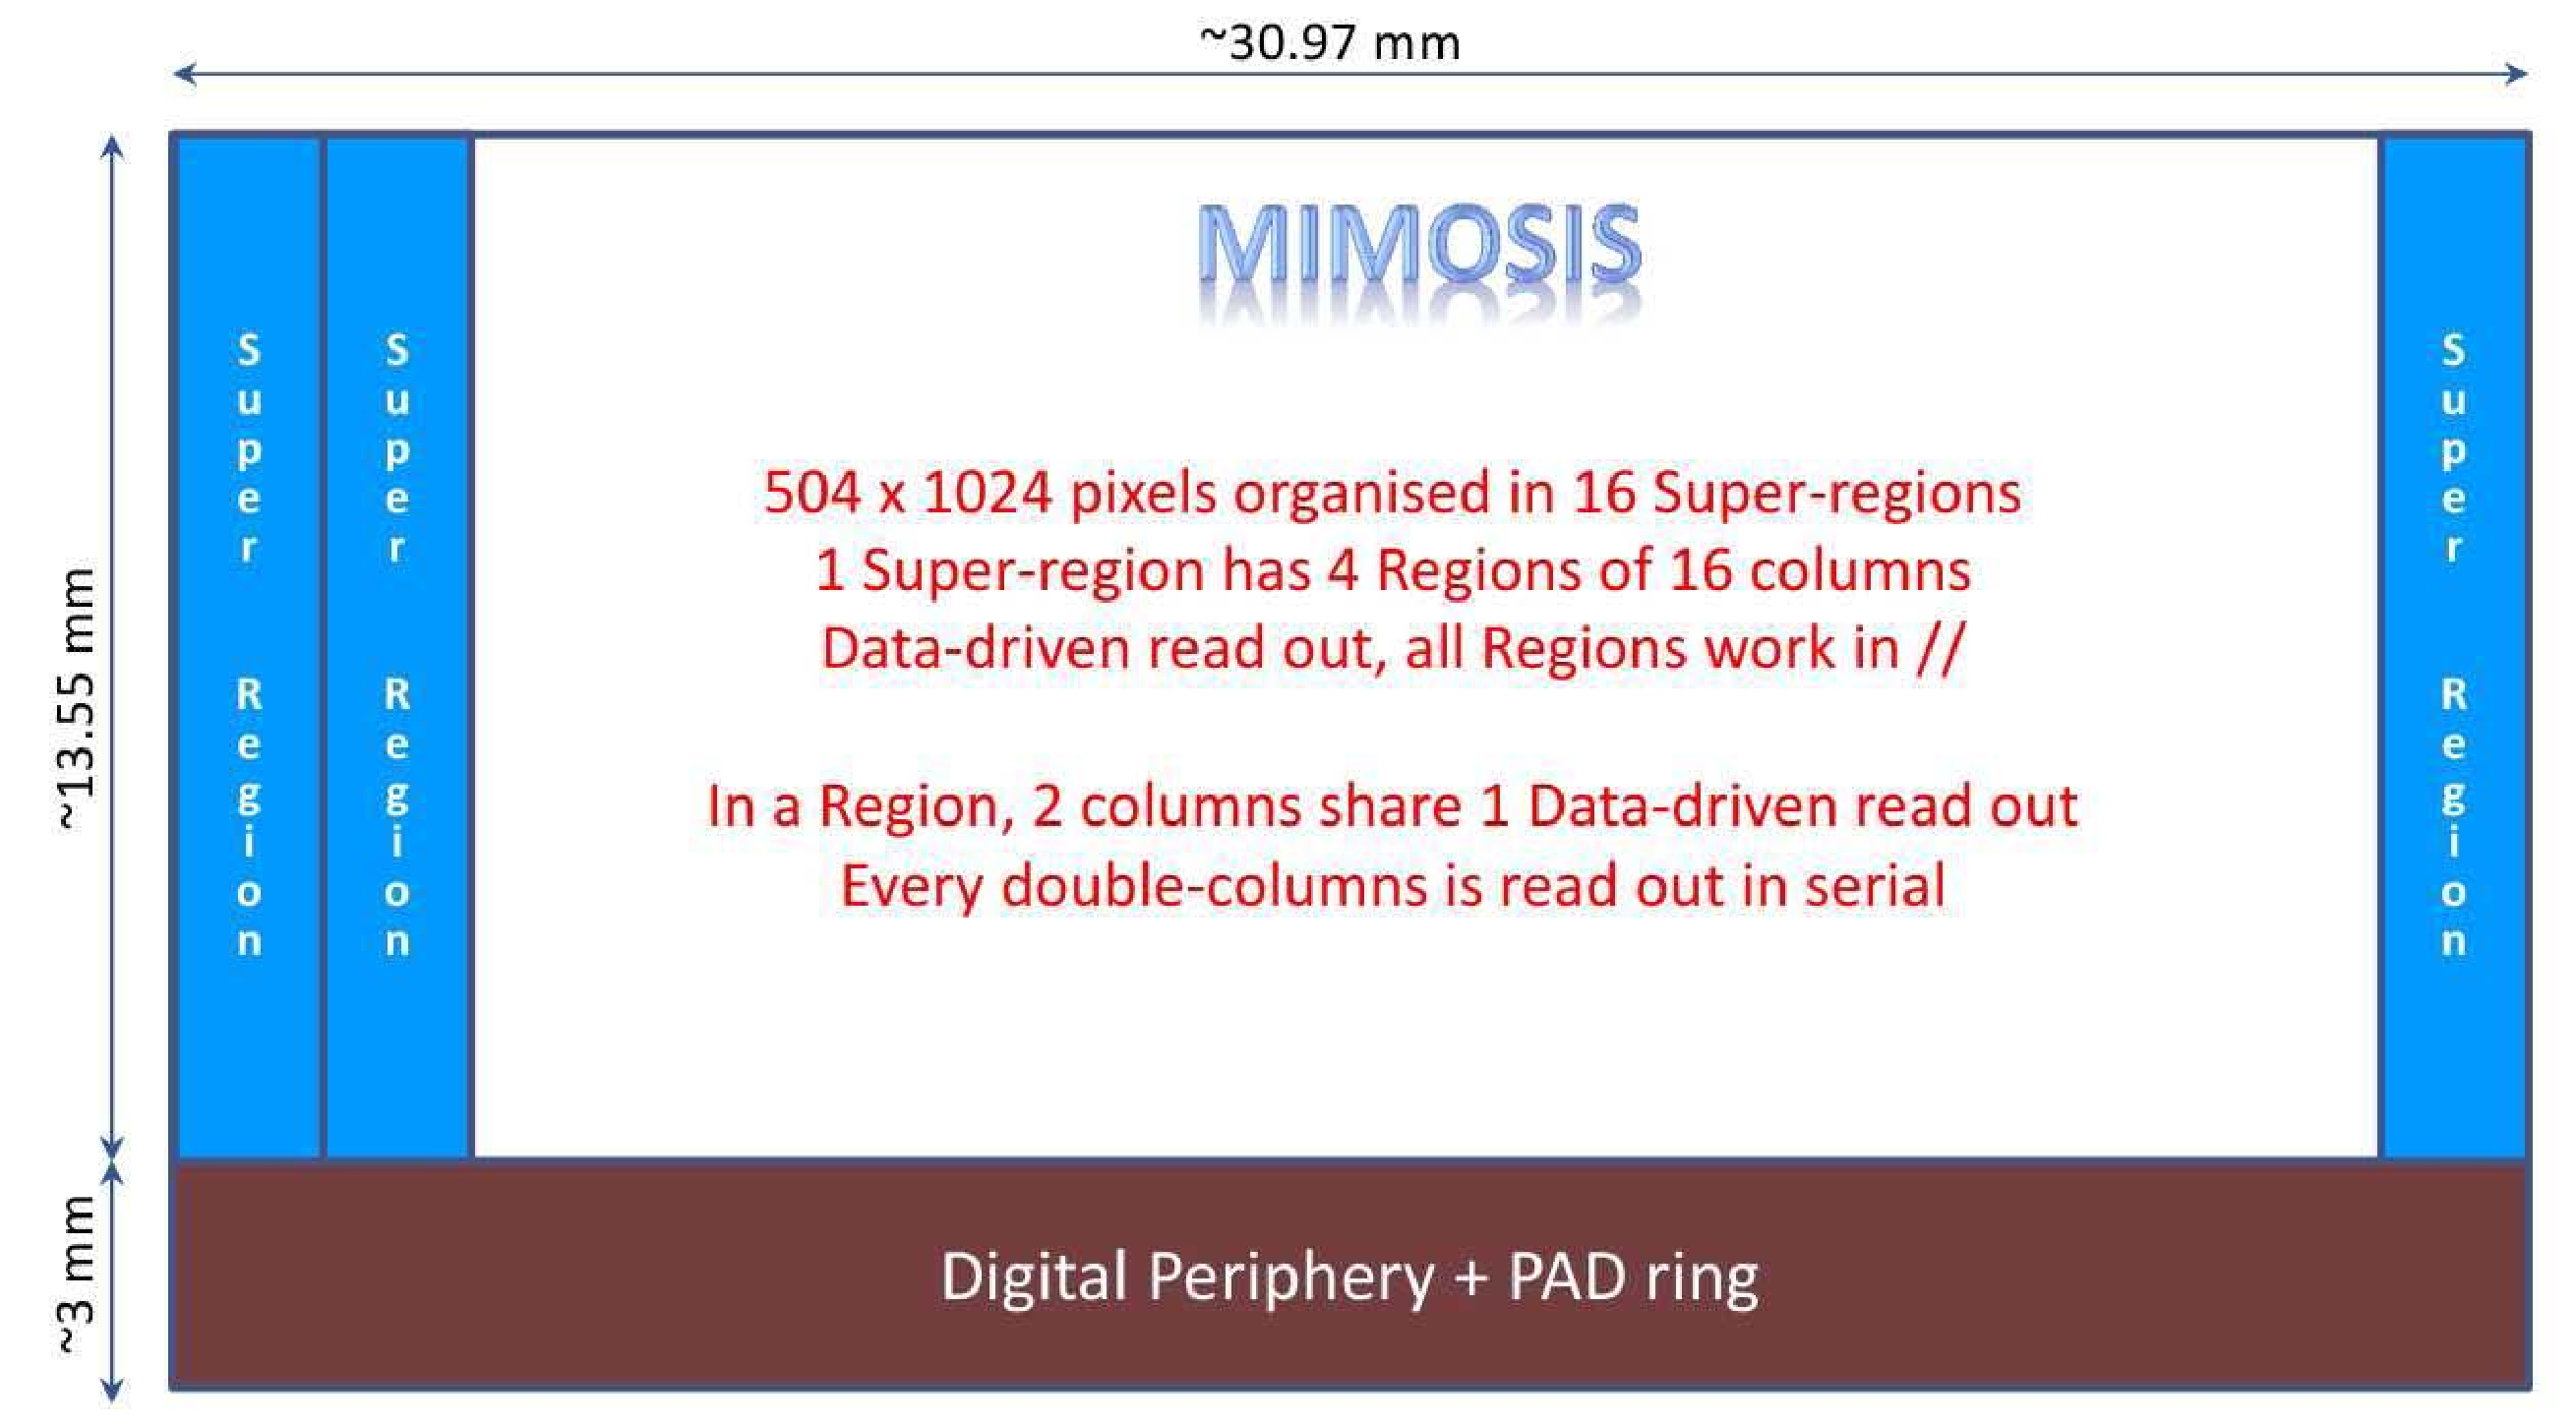
\includegraphics[width=.7\linewidth]{VertexDetector/CMOS/CHG-slide4.pdf}
	\caption{Schematic representation of the MIMOSIS sensor developed to equip the CBM-MVD.}
	\label{fig:VertexDetector:CMOS:MIMOSIS}
\end{figure}

\begin{figure}
	\centering
	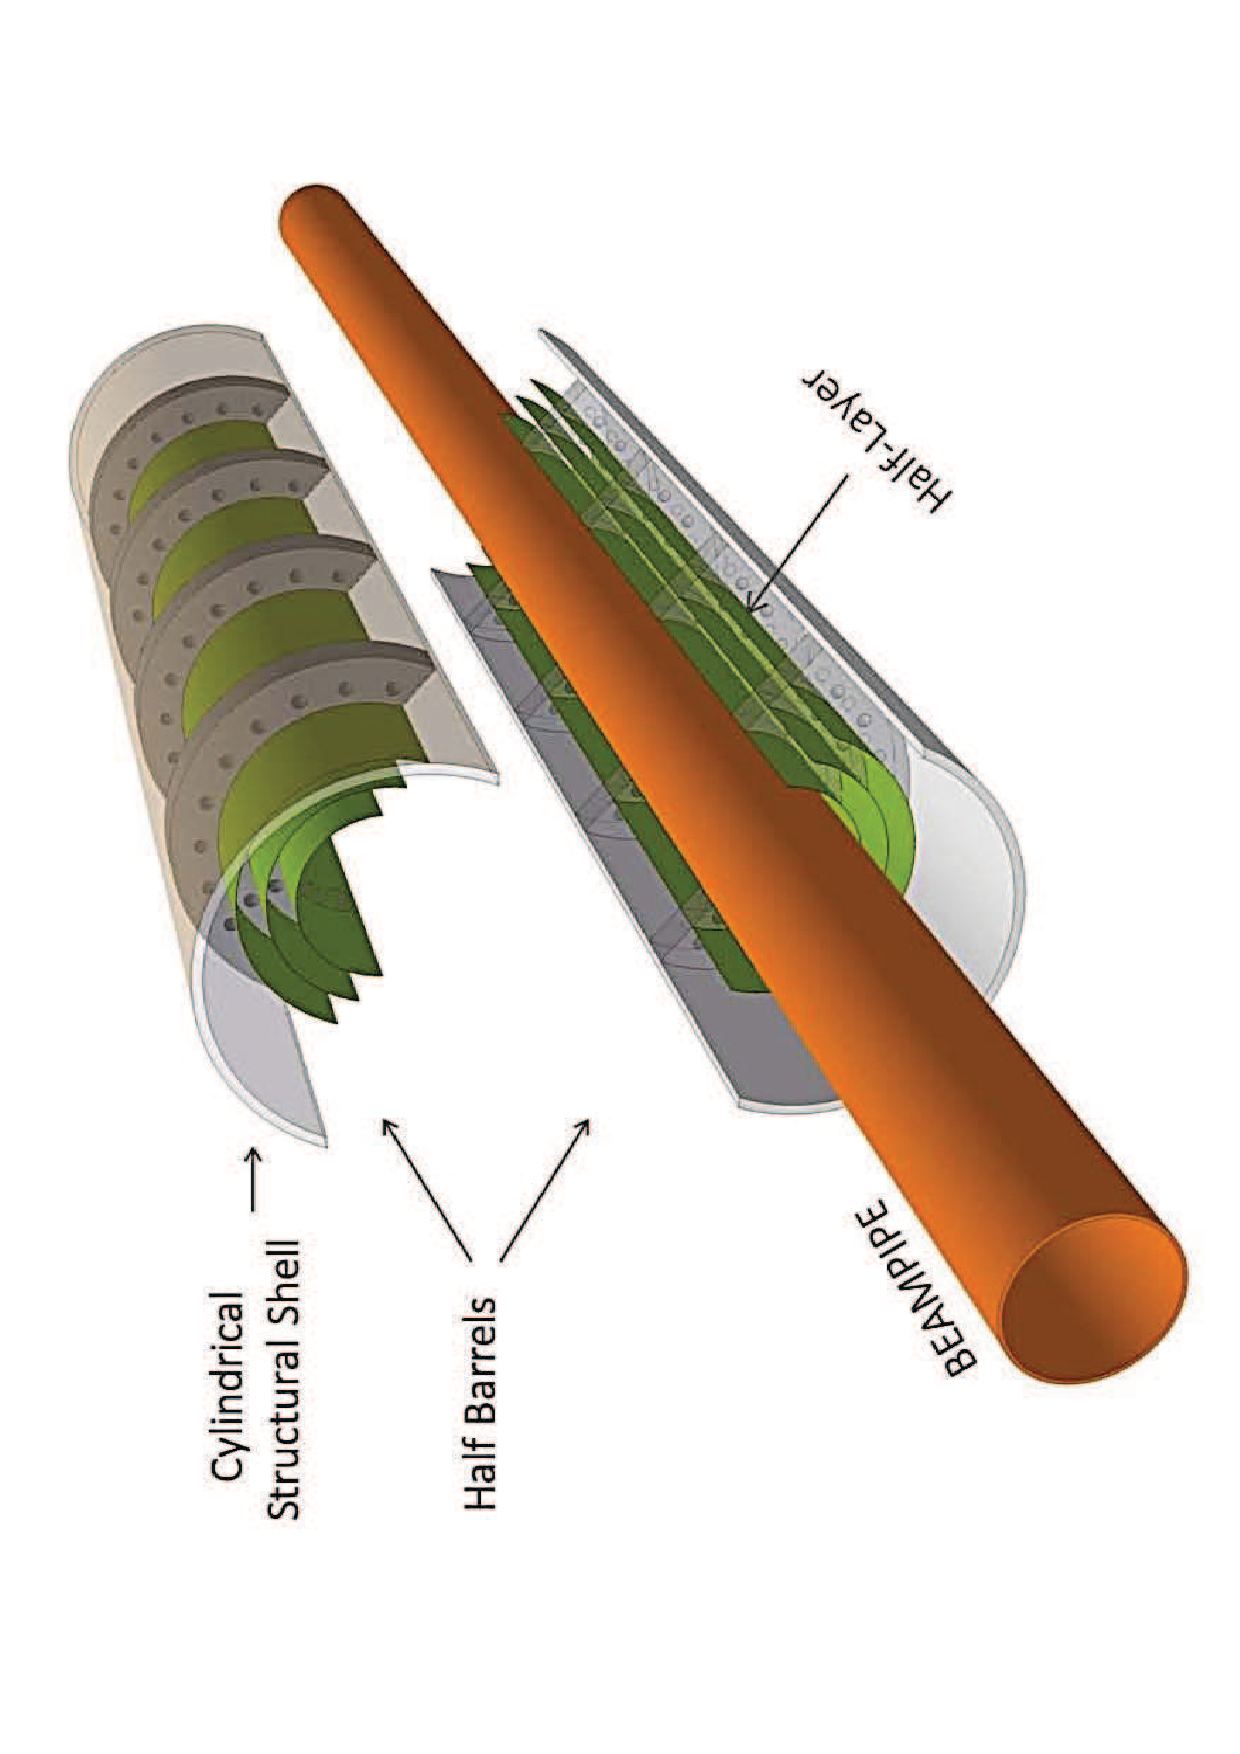
\includegraphics[width=.5\linewidth]{VertexDetector/CMOS/ALICE-Vertex-Stitched.pdf}
    \caption{Schematic view illustrating the concept of a vertex detector based on stitched sensors curved according to a cylindrical geometry.}
	\label{fig:VertexDetector:CMOS:stitching}
\end{figure}

Another important step achieved in recent years is the first operation 
of ultra-light double-sided pixelated ladders in a real experimental 
environment, based on two PLUME devices installed near the interaction 
region of the BELLE-II experiment during the beam commissioning phase 
called BEAST-II~\cite{CUESTA2020163862}. The ladders were ran successfully 
through the period, contributing to the monitoring of the background 
induced by SuperKEKB in the inner tracker volume with their \SI{3.3}{\micro\meter}
single point resolution and their low material budget ($\sim$ \mbox{0.4\% X$_0$}),
despite their modest read-out speed (\SI{115}{\micro\second}).   


Squeezing the material budget of the double-sided PLUME ladders to 
$\lesssim~0.3\%~X_0$ remains of prime interest but represents a major engineering challenge, possibly complicated by the necessity to 
power pulse ladders in the strong experimental magnetic field. 
Power pulsing is suspected to be needed in case of continuous 
read-out with the present sensor design, derived from MIMOSIS. 
However, whether it will be needed for all layers and for a sensor
fabrication process with smaller feature size remains an open 
question. Moreover, the possibility to introduce micro-channel 
cooling in the ladders will also be considered in order to mitigate 
power pulsing requirements.

Another engineering challenge may follow from the possibility 
to realise wafer scale sensors benefitting from the stitching
proposed by CMOS foundries for commercial imagers (see the next
subsection). In this case, the sensors would be curved to form 
large parts of a cylinder and would need a specific mechanical
concept to ensure rigidity and low mass cooling services.  

\subsection{Future Plans}
The achieved performances, which may already be considered as 
relatively satisfactory, are anticipated to be boosted in the 
coming years by industrial progress, following in particular 
from evolutions of the ASIC production technology, which drives 
steady miniaturization of integrated circuits. CMOS foundries 
also offer the possibility of stitching, which allows for 
wafer-scale sensors. Once thinned to a few tens of microns, 
the sensor may be curved according to a cylindrical surface, 
with a sizeable gain in stiffness. A few sensors only are then 
required to equip a complete detector layer, with a drastic 
suppression of mechanical support material consecutive to the 
disappearance of overlaps between neighboring detector modules. 
This concept is promoted by the ALICE collaboration, which aims 
for an upgrade of its vertex detector~\cite{CERN-LHCC-2019-018}. Maximum 
benefit is expected for the innermost detector layer, where the 
beam pipe may act as a mechanical support. 

  Stitching is available in the \SI{180}{\nano\meter} CMOS process used for 
ALPIDE and MIMOSIS. It is also accessible in a forthcoming 65~nm 
imaging process investigated at CERN within a partnership involving 
groups interested in various applications, including ILC related 
tracking devices. The process should in particular allow for 
reduced pixel dimensions, and therefore improved single point 
resolution. Overall, the evolution toward this \SI{65}{\nano\meter} CMOS process 
is particularly appealing and should take advantage from a 
cross-fertilization between numerous projects.

  Another promising R\&D direction addresses the realization of 
two-tier chips interconnected at the pixel level through industrial 
micro-bonding techniques. High-density micro-bonding is getting 
widespread, which allows to distribute the analog front-end and 
the digital circuitry of a pixel among two different chips being 
ultimately interconnected at the pixel level. The result is a 
reduced pixel size which improves the spatial resolution and 
enhances the data compression. A micro-bonding process already 
successfully tried with SoI sensors, is getting explored with CPS.

\section{DEPFET Pixel Sensors}
\label{sec:DEPFET}
Most recent update: 2020-01-28\\
Contact person: Marcel Vos (email: vos@ific.uv.es)

\subsection{The DEPFET Collaboration}
\href{http://www.hll.mpg.de/twiki/bin/view/DEPFET/CollaborationList}{The DEPFET R\&D collaboration} consists of nearly 100 members from 13 institutes. This collaboration develops active pixel detectors with in-pixel amplification embedded in a fully depleted detector-grade silicon sensor, for application in $e^+e^-$ colliders such as SuperKEKB and the ILC. DEPFET detectors are also developed for imaging applications in telescopes~\cite{Baehr:2018zbc,Treberspurg:2018nwm} and light sources and for dark matter direct detection experiments~\cite{Baehr:2017lmu}.

The collaboration currently takes responsibility for the following work packages:
\begin{description}
\item[Mechanics] {The DEPFET ladder integrates the support structure with the sensor wafer using state-of-the-art silicon processing technology. Read-out electronics and signal routing are integrated on the silicon wafer. The resulting all-silicon ladder is fully self-supporting. The mechanical properties of thin ladders in a realistic environment are studied in detail using detailed models (mock-ups) for Belle II and the ILC .}
\item[Cooling] {The DEPFET cooling concept for Belle II relies on two-phase \ce{CO2} cooling for the end-of-ladder. The sensor is cooled moreover with a forced flow of cold gas. The \ce{CO2} cooling plant is developed by KEK, while the design for the cooling block/support structure is performed within the collaboration. The impact of the linear collider cooling strategy - based on reducing the power dissipated using a pulsed power supply to the detector and cooling through a forced air flow - is studied. A novel cooling strategy for future applications based on mico-channels in the sensors~\cite{Vos:2017uin,Andricek:2016rsq} is being developed, in collaboration with the AIDA2020 project funded under the H2020 framework program of the EU. Solutions for monitoring of environmental parameters are being developed.}
\item[Ancillary ASICs] {The operation of a DEPFET detector requires ancillary electronics in the form of a read-out ASIC (the Drain Current Digitizer), a steering ASIC (SWITCHER) and on-detector ASICs for digital data processing (DHP). These ASICs are developed within the collaboration.}
\item[Data Acquisition and Trigger] {The development of off-detector electronics to process the data from the Belle II vertex detector.}
\item[Characterization of prototypes, laboratory and beam tests] {This work package has contributions from nearly all institutes involved in the DEPFET collaboration.}
\end{description}

Currently, the construction of the Belle II vertex detector~\cite{Abe:2010gxa} is the main focus of the collaboration. The requirements of the Belle II vertex detector are similar to those of the ILC, and more stringent in some aspects. The Belle II construction project therefore has considerable synergy with developments for a future linear collider. A second vertex detector for Belle II, to be installed in 2021-2022, is under construction at the time of writing. Several groups have started to develop ideas for an upgrade of the Belle II vertex detector on a longer time scale. The LC-specific effort is focused on the development of small-pixel devices and the design of a forward vertex detector. 

\begin{figure}
    \centering
    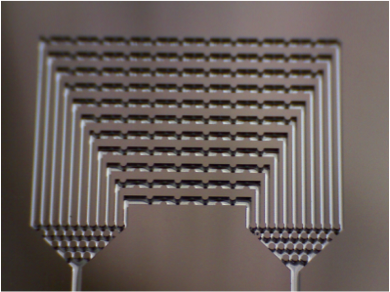
\includegraphics[width=.3\linewidth]{VertexDetector/DEPFET/microChannel}
    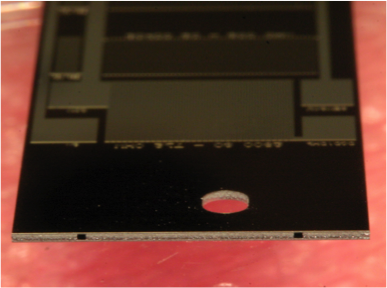
\includegraphics[width=.3\linewidth]{VertexDetector/DEPFET/microChannelSamples}
    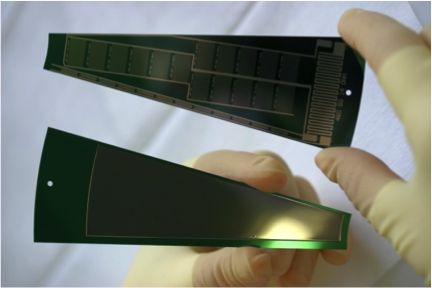
\includegraphics[width=.3\linewidth]{VertexDetector/DEPFET/FTD_Mockup}
    \caption{left: Microchannel cooling. center: Samples with cooling circuits. right: FTD mockup}
    \label{fig:VertexDetector:DEPFET}
\end{figure}

\subsection{Introduction}
The DEPFET technology implements amplification within the active pixel by integrating a p-MOS transistor in each pixel on the fully depleted high-resistivity silicon wafer. Additional n-implants near the transistor act as a trap for charge carriers created in the substrate (internal gate), so that they are collected beneath the transistor gate. The amplified signal is extracted from the pixel matrix by a numbers of ASICs~\cite{Kishishita:2014maa,Krueger2010337} mounted directly on the sensor: The SWITCHER, Drain Current Digitizer (DCD)~\cite{1748-0221-6-01-C01085,5446501} and Data Handling Processor (DHP)~\cite{1748-0221-7-01-C01069}.

The DEPFET in-pixel amplification allows for a comfortable signal-to-noise ratio with a very thin active detector. The reduced sensor thickness of $\SI{75}{\micro\meter}$ for Belle II, $\SI{50}{\micro\meter}$ for the Linear Collider, is the key to remain within the material budget of 0.15\% of a radiation length per layer. DEPFET prototypes with $20\times\SI{20}{\micro\meter\squared}$, small enough to meet the stringent spatial resolution specifications of the ILC, have successfully been operated in beam tests~\cite{Andricek:2011zza,Velthuis:2008zza}. The DEPFET matrix is read out in rolling shutter mode at a rate of 100 ns/row. For the column depths relevant for the ILC and Belle II a frame rate of several tens of $\si{\micro\second}$ is achieved~\cite{6484214}. The expected performance of a DEPFET-based vertex detector meets the specifications drawn up by the ILD experiment. DEPFET is also considered as a back-up solution to the SiD concept, in case the single bunch crossing time stamping proves to be out of reach.

\begin{table}
\centering
\caption{Comparison of ILC and Belle II requirements of a vertex detector}
\label{tab:Vertex:DEPFET:ILCBelleComparison}
\begin{tabular}{ccc}
    & ILC & Belle II \\
    \hline
    occupancy & 0.13 hits/\si{\micro\meter\squared}/s & 0.4 hits/\si{\micro\meter\squared}/s \\
    radiation & $< \SI{100}{krad/yr}$ & $> \SI{1}{Mrad/yr}$  \\
    & $\SI{e11}{MeV n_{eq}/yr}$ & $2\times \SI{e12}{MeV n_{eq}/yr}$ \\
    duty cycle & 1/200 & 1 \\
    frame time & $25-\SI{100}{\micro s} $ & $\SI{20}{\micro s}$ \\
    momentum range & 100 keV - 500 GeV & $ < \sim\SI{1}{GeV}$ \\
    angular acceptance & 6\degree - 174\degree & 17\degree - 150\degree \\
    spatial resolution & excellent: $3-\SI{5}{\micro\meter}$ & moderate \\
    pixel size & $20\times \SI{20}{\micro\meter}$ & $50\times \SI{75}{\micro\meter}$ \\
    material budget & 0.15\% $X_0$/layer & 0.21\% $X_0$/layer \\
\end{tabular}
\end{table}

\subsection{Recent Milestones}
The concept of a DEPFET active pixel detector for vertex detection at collider experiments was initiated in the linear collider community (for TESLA).
The operation principle was extensively proven~\cite{Andricek:2011zza,Velthuis:2008zza} on small-scale prototypes. A recent reassessment of the DEPFET potential for a linear collider at the energy frontier is found in~\cite{6484214} and in the report~\cite{depfet:ecfaReport} for the ECFA detector R\&D review in 2014.
A large-scale, \SI{75}{\micro\meter} thin Belle II ladder with the ancillary ASICs integrated on the sensor was successfully submitted to a test in an electron beam at DESY in January 2014\cite{Marinas:2014iza}. The Belle II vertex detector was integrated in the experiment in 2018 and is currently operating and contributing to physics data~\cite{Schwenker:2017kcf,Paschen:2019sit,Abudinen:2019rkl}. 


The first full-scale DHP prototype was implemented in IBM \SI{90}{nm} CMOS technology. As this technology was discontinued, more recent designs were submitted in the TSMC \SI{65}{nm} CMOS process. DHPT v.1.0 comprises temperature independent current references, 11 bias 8-bit DACs with current output, an integrated temperature measuring system and JTAG control. This design has been successfully tested during early 2014\cite{Kishishita:2014maa}.

\subsection{Engineering Challenges}
Vertex detector ladders with a thickness of several tens of microns and a spatial resolution of well below \SI{10}{\micro\meter} require very robust mechanical properties. The power generated by the sensors and ASICs must be removed with the smallest impact on the detector material.
Measurements on thin ladders under a realistic load, including pulsed powering according to the ILC beam structure, prove the excellent mechanical properties of the all-silicon ladder~\cite{thermomech}.

\subsection{Future Plans}
Currently, the operation of the Belle II vertex detector (installed 2018) implies a large effort of the collaboration. Specific developments that are required for the ILC are:
\begin{itemize}
\item Development of large-scale prototypes with the required small pixel size  ($20 \times \SI{20}{\micro\meter^2}$). This is partially synergetic with a possible Belle II vertex detector upgrade.
\item Development of prototypes with improved read-out speed, by a more parallel read-out of the pixels.
\item Design of the ancillary ASICs, taking full responsibility for future design cycles of the Front End read-out chip, the Drain Current Digitizer (DCD) that is relevant to the ILC and a Belle II upgrade. This chip converts the analog signal from the detector to digital and has a crucial impact on the detector performance.
\item Development of a concept for mechanical support and cooling compatible with operation in the ILD and SiD detectors, with minimal material over the acceptance down to a polar angle of approximately 8 degrees.
\item Creation of an engineering design for a DEPFET all-silicon module with the required petal geometry for the Forward Tracking Disks.
\end{itemize}

Important experience is gained in the construction and operation of the Belle II vertex detector, and with the thermal and mechanical properties of ultra-thin ladders. Measurents on thin ladders under a realistic load, including pulsed powering according to the ILC beam structure, prove the excellent mechanical properties of the all-silicon ladder.

\section{FPCCD}
Most recent update: 2018-06-07 \\
Contact person: Yasuhiro Sugimoto (email: yasuhiro.sugimoto@kek.jp)
\subsection{Introduction}
    Fine pixel CCD (FPCCD) is one of the candidate sensor options for the vertex detector of the ILD detector at the ILC~\cite{Sugimoto:2005ru,2009arXiv0902.2067S,2012arXiv1202.5832S}. In the present design, FPCCD sensors for the innermost layer of the vertex detector have a pixel size of \SI{5}{\micro\meter} and a fully depleted epitaxial layer with a thickness of \SI{15}{\micro\meter}. Because of the small size of the pixels, the occupancy is acceptably low even if the hits are accumulated for one nominal ILC bunch train ($\approx\SI{1}{ms}$).
    The efforts of the FPCCD collaboration are currently focused on pixel characterization and development, while we also pursue developments to the cooling system, electronics downstream of ASICs and the reconstruction software~\cite{Mori:2014xta}.
\subsection{Recent Milestones}
R\&D activity for the FPCCD vertex detector at present is mainly focused on FPCCD sensors and a detector cooling system using 2-phase \ce{CO2}.
One of the achievements of FPCCD sensors after DBD is the fabrication of real size ($12.3 \times \SI{62.4}{\mathrm{mm}^2}$) sensors with \SI{50}{\micro\meter} total thickness. Figure~\ref{fig:FPCCD:realSizeSensor} shows the real size prototype sensor. It has 8 readout nodes, and each channel has different pixel sizes of \SI{12}{\micro\meter}, \SI{8}{\micro\meter}, and \SI{6}{\micro\meter}.

\begin{figure}
 \begin{minipage}{0.49\textwidth}
    \centering
    \includegraphics*[width=\textwidth,keepaspectratio]{VertexDetector/FPCCD/realSizeFPCCDSensor.png}
    \caption{Real size FPCCD sensor thinned down to \SI{50}{\micro\meter}}
    \label{fig:FPCCD:realSizeSensor}
 \end{minipage}
 \hfill
 \begin{minipage}{0.49\textwidth}
    \centering
    \includegraphics*[width=\textwidth,keepaspectratio]{VertexDetector/FPCCD/coolingSystemSchematic.png}
    \caption{A simplified schematic diagram of the two-phase $\text{CO}_2$ cooling system}
    \label{fig:FPCCD:coolingSystemSchematic}
 \end{minipage}
 \end{figure}

We have started a neutron damage test using small ($\SI{6}{mm}\times\SI{6}{mm}$) FPCCD prototypes~\cite{lcws:fpccd:ito:2013,Murai:2017pyh}. A prototype sensor was irradiated by a neutron beam of few tens of MeV at the CYRIC facility of Tohoku University. The detailed analysis on the irradiated sensor is still on-going.
In order to increase the radiation immunity of FPCCD sensors, particularly to reduce the transfer inefficiency due to radiation damage, the sensors should be cooled down to \SI{-40}{\degree C}. We have started R\&D on a two-phase \ce{CO2} cooling system for this purpose. There are several examples of utilizing two-phase \ce{CO2} cooling systems for high energy physics experiments. For these cases, the \ce{CO2} coolant is circulated using liquid pumps. This method is, however, not so efficient for very low temperature cooling of \SI{-40}{\degree C}. Therefore, we adopted a \ce{CO2} gas compressor for the circulation of \ce{CO2} coolant. Figure~\ref{fig:FPCCD:coolingSystemSchematic} shows a simplified schematic diagram of the system. A prototype system has been constructed, and cooling between \SI{-40}{\degree C} and \SI{+15}{\degree C} has been successfully demonstrated using this system.

\subsection{Engineering Challenges}
    In the present design of the ILD vertex detector, two sensor layers are mounted on both sides of a light-weight ladder of ~\SI{2}{mm} thickness. Our goal of the material budget of this ladder is 0.3\% X0/ladder = 0.15\% X0/layer. This goal would not be so easy to accomplish, and we need a lot of R\&D effort.
    The ladders have to be cooled down to \SI{-40}{\degree C}. We plan to achieve this cooling by heat conduction to the end-plate on which thin cooling tubes for 2-phase \ce{CO2} are attached. The design of this structure is not trivial, and we need R\&D including thermal simulation.
    There are challenges both with the mechanical structure and the electronics circuit for the ladder R\&D. We have not started this effort yet.
\subsection{Future Plans}
    We have been doing our R\&D on the FPCCD vertex detector based on a Grant-in-aid for science research which expires at the end of FY2015. By that time, we plan to carry out the following R\&D items:
\begin{itemize}
    \item Characterization of FPCCD sensors including beam tests and radiation damage tests
    \item Development of FPCCD sensors with the pixel size of \SI{5}{\micro\meter}, which is our ultimate goal
    \item Construction of prototype ladders for inner layers
    \item Development of readout electronics downstream of ASICs
\end{itemize}
If new funding is secured in future, the following R\&D items have to be done:
\begin{itemize}
    \item Development of larger FPCCD sensors and prototype ladders for outer layers
    \item Development of readout electronics which can fit in the small space of real experiment
    \item Construction of a real size engineering prototype and its cooling test
\end{itemize}

\section{ChronoPixel}
Most recent update: 2015-11-11 \\
Contact person: Jim Brau (email: jimbrau@uoregon.edu)
\subsection{Introduction}
The ChronoPixel is a monolithic CMOS pixelated sensor with the ability to record up to two time stamps of pixel hits by charged particles in a nominal ILC bunch train. This information is read out in the time interval between bunch trains. The ChronoPixel option for the ILC vertex detector was described in the ILC DBD~\cite{2011arXiv1109.2811B}. By the time of the DBD, 2 prototypes had been built and tested, and the summary of test results was also presented in the DBD. The main points are:

\begin{figure}
    \centering
    \begin{minipage}[t]{0.35\textwidth}    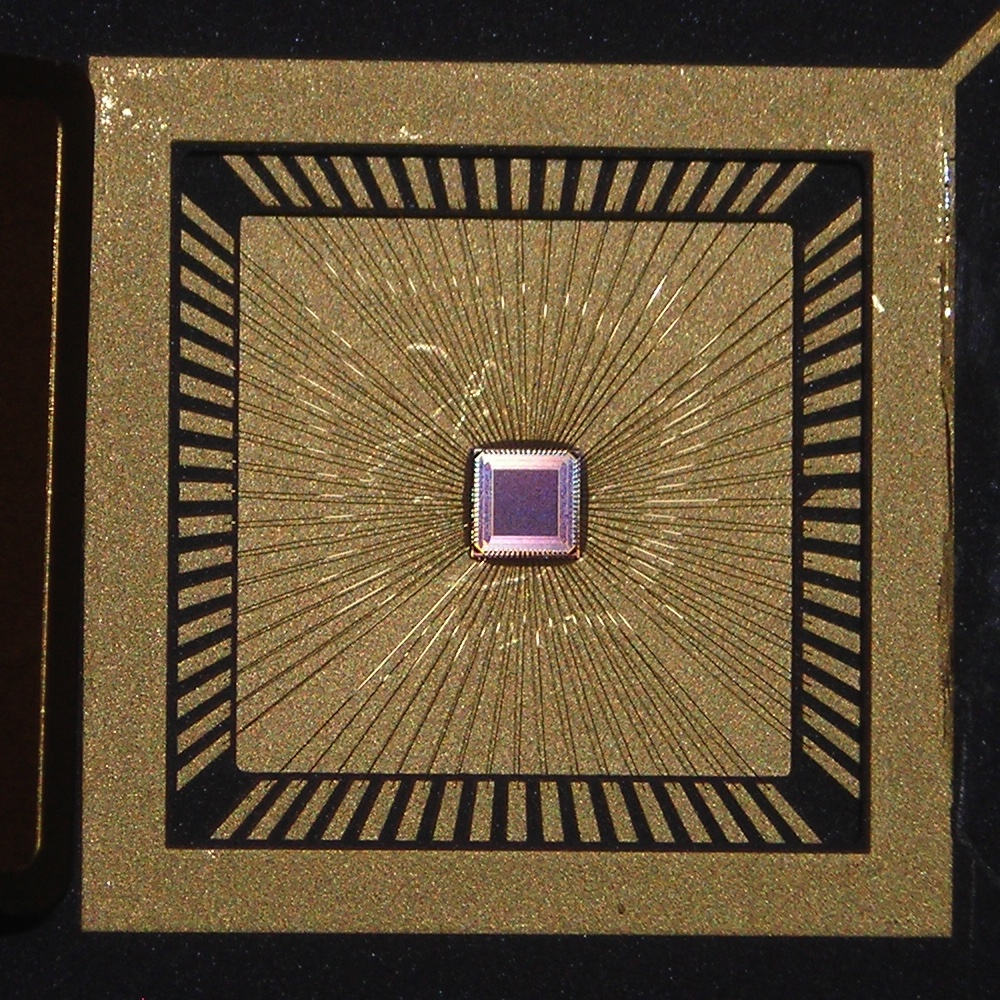
\includegraphics[width=\linewidth]{VertexDetector/Chronopix/Chronopix_image}
    \caption{Photograph of the prototype 3 chip in its package. The chip has $48\times48$ pixels, each with a size of $25\times\SI{25}{\micro\meter^2}$.}
    \label{fig:VertexDetector:ChronoPixel:image}
\end{minipage}\quad
\begin{minipage}[t]{0.35\textwidth}
    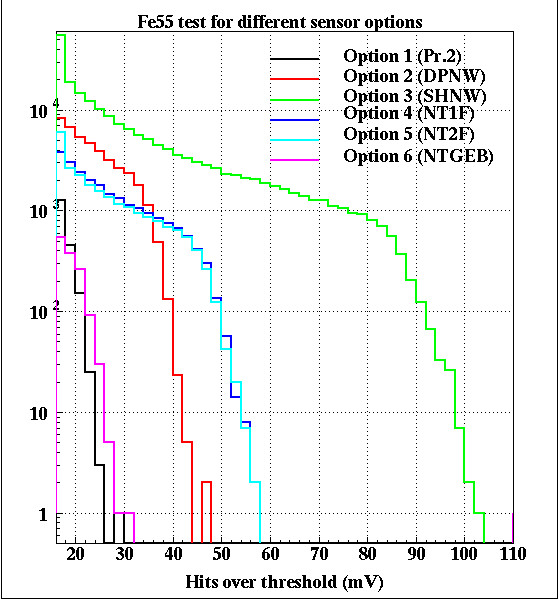
\includegraphics[width=\linewidth]{VertexDetector/Chronopix/Fe55tst}
    \caption{\ce{^{55}Fe} signal over threshold counts for 6 different sensor diode options,
implemented in prototype 3. For comparison, option 1 is the same as in prototype 2.}
    \label{fig:VertexDetector:ChronoPixel:Fe55Response}
\end{minipage}
\end{figure}

\begin{itemize}
    \item We have proven that we can record time stamps in every pixel with time resolution down to \SI{150}{ns}.
    \item We have tested sparse readout, allowing to read only pixels with hits, thus reducing readout time to the level allowing readout of all pixels in the sensor in the intervals between bunch crossings.
    \item We have tested pulsed power for the analog part of the pixels and have proven~\cite{sinev:Chronopix:FirstPrototype} that turning power ON about \SI{100}{\micro\second} before bunch train and turning it off between bunch trains does not create any problems for threshold setting accuracy in the comparators.
    \item We have measured sensor noise level, including all pick-up and cross-talk. It was 24 e- r.m.s in prototype 1 and 26 e- r.m.s. in prototype 3, sensor option 3. Our specification was 25 e- noise.
    \item We have tested the idea of building all in-pixel electronics only from NMOS transistors, thus eliminating the need for a special process (deep p-well) to protect signal charge from parasitic collection by in-pixel transistors. We have proven~\cite{sinev:Chronopixel:RnDstatus2013} that all NMOS electronics can be built in this way, and that this does not significantly increase the power consumption compared to CMOS electronics.
    \item We have tested the compensation of comparator offsets using analog calibration, when the value of the offset is stored as a voltage on the capacitor in each pixel. This has an advantage over digital calibration (where the offset value is stored as code in the special register) in that there are no discrete levels, and the accuracy of such a calibration scheme is not affected by the size of the register or the spread of the initial offsets.
\end{itemize}

\subsection{Recent Milestones}
\begin{itemize}
    \item Test of prototype 2 revealed some problems. Possible solutions for these problems were discussed with Sarnoff engineers.
    \item A new contract with Sarnoff for the design of prototype 3 was signed in August 2013.
    \item Prototype 3 was manufactured in September 2014. Tests have shown that problems revealed in prototype 2 were solved.
\end{itemize}
The most recent report~\cite{sinev:POS:Vertex2105} on the status of ChronoPixel was presented by N.~Sinev in June 2015 at Vertex2015 in Santa Fe, New Mexico.

\subsection{Engineering Challenges}
\begin{itemize}
    \item The Vertex Detector for ILC faces many engineering challenges. The sensors need to be thinned to about \SI{50}{\micro\meter} to reduce the amount of material in the detector. Support structures also need to be very light, but provide enough stability. Power dissipation of the entire detector should be small to be able to use only air cooling.
    \item If acceptable levels of the sensor diode capacitance can be achieved, the signal-to-noise ratio will improve. However, a lower value of the capacitance will make the pixels more sensitive to cross-talk through capacitive coupling. Reducing this coupling can be a challenge.
    \item Transition from small prototypes (few $\text{mm}^{2}$) to ILC detector size ($\approx \SI{10}{cm^2}$) may meet additional problems. One of them will be the effect of Lorentz forces on the power supply buses, especially in the case of power pulsing. Power pulsing is the only way to achieve acceptable power dissipation in the vertex detector. However, it will generate varying Lorentz forces, acting on power supply lines. This may produce vibrations, which are unacceptable for the required spatial resolution of the detector.
\end{itemize}

\subsection{Future Plans}
\begin{itemize}
    \item To achieve signal-to-noise ratio required for close to 100\% signal registration efficiency. We have achieved very low sensor capacitance in prototype 3, and the signal-to-noise ratio with such a sensor capacitance for \ce{^{55}Fe} signal is about 60, however, for minimum ionizing particles the signal will be much smaller, depending on epitaxial layer thickness and charge collection efficiency. The signal-to-noise ratio for standard \SI{7}{\micro\meter} epitaxial layer will be 20 if the charge collection efficiency is 100\%, which is unlikely (we have not measured it yet). So we probably will need to increase the epitaxial layer thickness.
    \item To achieve the required pixel size (prototype 3 has \SI{25}{\micro\meter} pixels, we would eventually like \SI{15}{\micro\meter}). It may require going to a technology with feature size less than \SI{65}{nm}. There seems to be no problems in that, but both -- good signal-to-noise ratio and pixel size requirements may be challenging.
    \item To achieve acceptable level of inter-pixel and digital-to-analog circuit cross talks and parasitic feedback.
    \item Depending on available funding, to build a complete sensor with a large enough area and full feature readout.
\end{itemize}

\section{3D Pixel Development}
Most recent update: 2016-04-30 \\
Contact person: Ron Lipton (email: lipton@fnal.gov)
\subsection{Introduction}
This R\&D area covers sensors and electronics integrated utilizing 3-dimensional electronics technology.  This technology is distinct from 3D sensors and builds on efforts in the electronics industry to stack multiple layers of electronics to form dense assemblies of complex devices.  It is important for Particle Physics in that it allows very fine pitch (\SI{4}{\micro\meter}) integration of sensors with multiple layers of electronics, allows interconnection to both the top and bottom of devices, and provides techniques for low mass, thinned devices. The interconnection of top and bottom means that sensors can be bonded to complex electronics with no wasted area for interconnect and optimal delivery of power and ground.

\begin{figure}[hb]
    \centering
    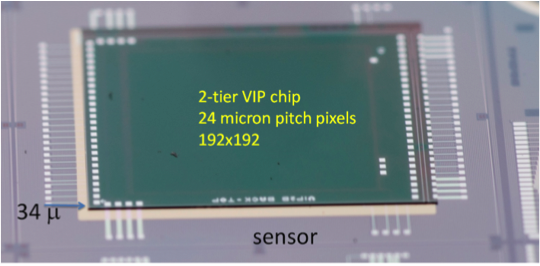
\includegraphics[width=.57\textwidth]{VertexDetector/VIP/ILCChip}
    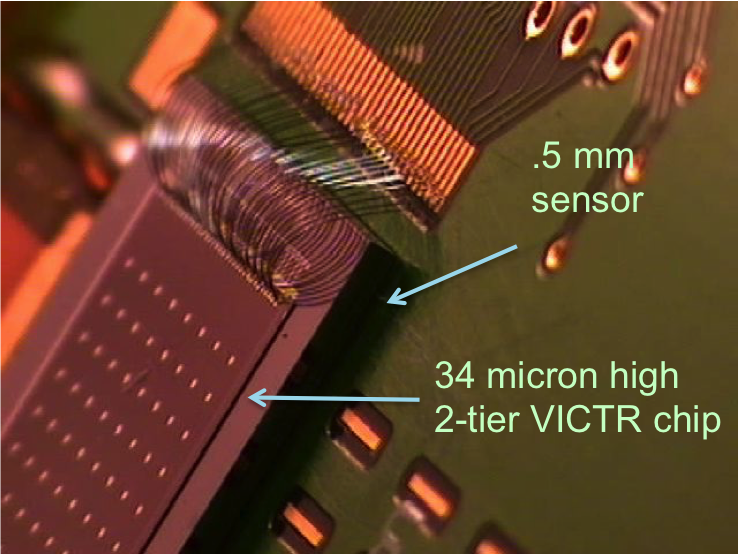
\includegraphics[width=.37\textwidth]{VertexDetector/VIP/CMSChip}
    \caption{Left: ILC Chip. Right: CMS chip}
    \label{fig:VertexDetector:VIP:variants}
\end{figure}

\subsection{Recent Milestones}
We have completed our multi-year effort to demonstrate commercial 3D technology. This consists of two tiers of \SI{0.13}{\micro\meter} CMOS interconnected with Direct Oxide Bonding (DBI) technology and access using Through-Silicon-Vias (TSV). The DBI bonds are at \SI{4}{\micro\meter} pitch. Fermilab sponsored the first 3D multi-project run for Particle Physics. The wafers were delivered last summer. Fermilab had three chips on the run: VICTR -- a CMS track trigger chip, VIPIC -- an X-ray imaging chip, and VIP -- an ILC vertex chip. Tests of the VIPIC and VICTR have shown working devices.  Tests for the VIP chip were delayed due to lack of funding and personnel.  We have recently restarted this work and initial tests are promising with the readout token successfully passed through the VIP.

In addition to the development of the 3D chips we have also explored the use of DBI to connect the 3D electronics with sensors.  Brookhaven Laboratory fabricated a sensor wafer with regions that mate to the VIP, VIPIC and VICTR chips.  The chips are ground to expose the top TSVs and contacts are deposited. The assembly is then attached to a handle wafer and the TSVs which project from the other side are exposed.  Wafers are then process for DBI bonding and individual die from the 3D wafer are bonded to the sensor wafer.  Finally the top ``handle'' silicon is ground and etched to reveal the previously formed contacts.  The total thickness of the readout at the end of this process is about \SI{25}{\micro\meter} (Figure~\ref{fig:VertexDetector:VIP:chipsOnBNLWafer}). These wafers were received at the end of March 2014 and are being tested.
\begin{figure}[hb]
    \centering
    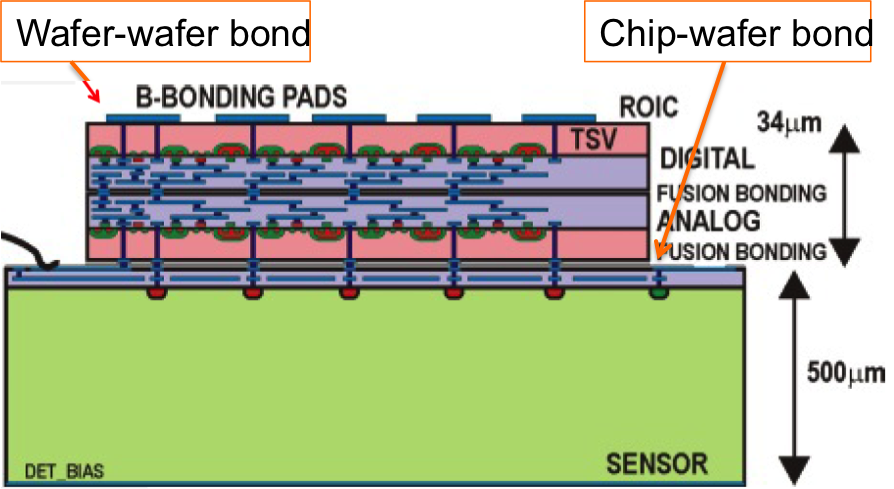
\includegraphics[width=.495\textwidth]{VertexDetector/VIP/schematic}
    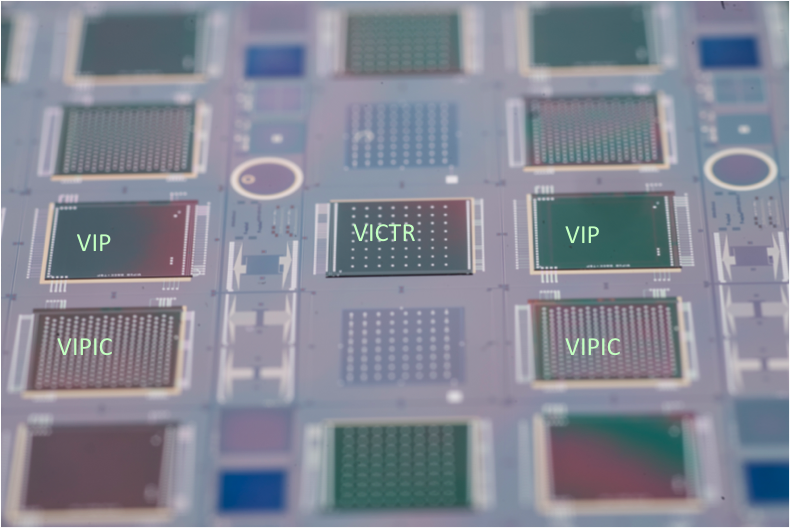
\includegraphics[width=.495\textwidth]{VertexDetector/VIP/3DChipsOnBNLWafers}
\caption{Left: Schematic view of the vertically integrated technology. Right: 3D chips placed on BNL sensor wafers. VIP is middle left and right}
\label{fig:VertexDetector:VIP:chipsOnBNLWafer}
\end{figure}
Due to the fact that contacts to a 3D assembly can be made to the body of the die, rather than its edge, no space needs to be reserved for wire bond contacts at the edge.  This raises the possibility of fabricating large, complex pixel detector arrays of 4-side butted devices using sensors with active edges.  We are in the process of demonstrating this technology utilizing active edge sensors fabricated at VTT and using wafer-to-wafer bonding to a 3D readout wafer. The active edge wafers are based on a silicon-on-insulator stack and thus can be fabricated with essentially arbitrarily thin sensors, in this case \SI{200}{\micro\meter}. Sensor and dummy readout wafers have been fabricated and a test wafer is being etched at SLAC. We expect to have DBI bonded assemblies this summer.

\subsection{Engineering Challenges}
Major  engineering challenges include:
\begin{itemize}
\item Development of widely commercially available 3D technologies.  Based partly on our development the silicon brokers CMP, CMC, and MOSIS now include 3D multi-project runs as part of their standard offerings.
\item Development of high yield 3D bonded chip-to-wafer devices.  This is the subject of our active edge project.
\item This development shares with other vertexing technologies the problems of low mass mechanical support, power delivery, and cooling. An SOI-based device can be made thin without special effort. Such thinned device will need low mass backing hybrid circuitry, presumably flex on carbon fiber or a similar technology
\end{itemize}

\subsection{Future Plans}
\begin{itemize}
\item Complete the 3D active edge project
\item Apply our concepts to x-ray imaging devices
\item ILC developments would await renewed funding in the US.
\end{itemize}


\begin{enumerate}
\item \fullcite{Deptuch:2013ona}
\item \fullcite{Yarema:2014mva}
\item \fullcite{MAJ:2013fwa}
\item \fullcite{2013arXiv1307.4301D}
\item \fullcite{1748-0221-7-12-C12010}
\item \fullcite{1748-0221-8-01-C01052}
\end{enumerate}

\section{SOI}
Most recent update: 2018-06-04 \\
Contact person: Yasuo Arai (email: yasuo.arai@kek.jp)
\subsection{Introduction}
\subsection{Recent Milestones}
At present, major issues in the SOI pixel development are ``back-gate effect'', ``hole trap under the transistors by radiation,'' and ``sensor-circuit cross talks'' as shown in Figure~\ref{fig:VertexDetector:SOI:SOI_Schematic}. For these, we have been developing a double SOI technology. The developed double SOI wafer has an additional middle-SOI(Si) layer under the transistors. The conduction layer of the middle-SOI can solve all the three issues. We could successfully process the double-SOI wafer (Figure~\ref{fig:VertexDetector:SOI:crossSectionAfterProcessing}). Threshold shift by radiations is successfully recovered by applying compensating voltage to the middle SOI layer (Figure~\ref{fig:VertexDetector:SOI:thresholdShift}).

\begin{figure}
	\begin{minipage}{0.49\textwidth}
		\centering     
		\includegraphics*[width=\textwidth,keepaspectratio]{VertexDetector/SOI/SOI_Schematic}
		\caption{Major issues in the SOI pixel detector and introduction of a middle-SOI layer}
		\label{fig:VertexDetector:SOI:SOI_Schematic}
 	\end{minipage}
 	\hfill
 	\begin{minipage}{0.49\textwidth}
 		\centering
    	\includegraphics*[width=\textwidth,keepaspectratio]{VertexDetector/SOI/crossSectionAfterProcessing}
		\caption{Cross section of the double SOI chip after processing}
		\label{fig:VertexDetector:SOI:crossSectionAfterProcessing}
 	\end{minipage}
 \end{figure}

\begin{figure}
	\centering
	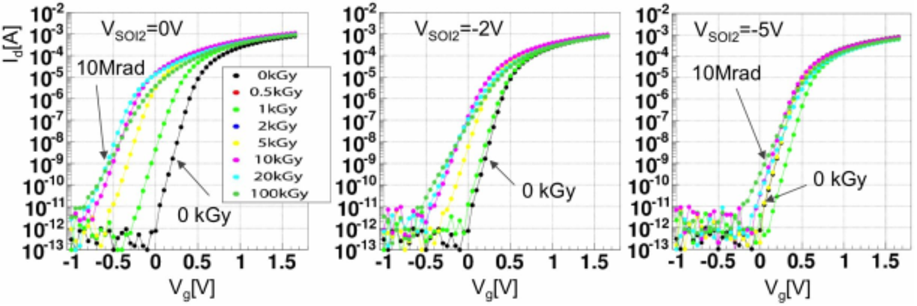
\includegraphics[width=.9\textwidth]{VertexDetector/SOI/thresholdShift}
	\caption{Threshold shift recovery by applying compensating voltage (Vsoi2) to the middle Si layer}
	\label{fig:VertexDetector:SOI:thresholdShift}
\end{figure}

\subsection{Engineering Challenges}
The impact parameter resolution for the ILC vertex detector is required to be a few \si{\micro\meter}. This means the pixel size must be less than about \SI{20}{\micro\meter\squared}. On the other hand, each pixel must register arrival time of the hits during bunch train, which requires many transistors and capacitors to be located in each pixel.
A solution to this is 3D vertical integration of the circuit layers. SOI technology is ideally suited for 3D integration, since the thinning is stopped at the buried oxide (BOX). We already tried 3D SOI pixel chip in collaboration with T-Micro Co. Ltd. The process flow of micro-bump 3D connection is shown in Figure~\ref{fig:VertexDetector:SOI:microbump3D}. This process achieves a resistance of ($\sim$\SI{0.3}{\ohm}/bump) between upper and lower tiers for 1,000 daisy chain (2,000 bumps) as shown in Figure~\ref{fig:VertexDetector:SOI:resistanceOfDaisyChain}.
However, to achieve the density of digital circuitry necessary for ILC operations, \SI{32}{nm} technology may be necessary for the upper tier in the ILC. This requires bonding of two different technology wafers. The 3D integration of different technology wafers (or chips) is still an engineering challenge.

\begin{figure}
	\begin{minipage}{0.35\textwidth}
		\centering
   		\includegraphics*[width=.5\textwidth,keepaspectratio]{VertexDetector/SOI/microBump3DIntegration}
		\caption{Micro-bump 3D integration process flow of the SOI pixel}
		\label{fig:VertexDetector:SOI:microbump3D}
 	\end{minipage}
 \hfill
 \begin{minipage}{0.64\textwidth}
 \centering
    \includegraphics*[width=\textwidth,keepaspectratio]{VertexDetector/SOI/BumpResistance.jpg}
	\caption{Resistance of micro-bump daisy chain between upper and lower tiers}
	\label{fig:VertexDetector:SOI:resistanceOfDaisyChain}
 \end{minipage}
 \end{figure}

\subsection{Future Plans}
Planned milestones for Detector R\&D:
\begin{itemize}
\item Sep. 2014 : Complete architecture study for the ILC pixel detector.
\item Mar. 2015 : Design and fabrication of first test chip for the ILC.
\item Dec. 2015 : Beam test of the test chip.
\end{itemize}

\section{CLICpix}
Most recent update: 2015-06-22 \\
Contact person: Dominik Dannheim (email: dominik.dannheim@cern.ch)

\subsection{Introduction}
 The precision physics needs at the CLIC TeV-scale linear electron-positron collider
require a vertex-detector system with excellent flavour-tagging capabilities through
a measurement of displaced vertices in an environment with high rates
of beam-induced background events~\cite{Miyamoto:1425915}.
As a result, the CLIC vertex-detector system needs to have excellent spatial resolution
(\SI{3}{\micro\meter}),
full geometrical coverage extending to low polar angles, extremely low material budget
(0.2\% $X_0$ per layer),
low occupancy facilitated by time-tagging (\SI{10}{ns} precision), and sufficient heat
removal from sensors and readout.
A concept based on hybrid pixel-detector technology is under development
for the CLIC vertex detector. It comprises fast, low-power and small-pitch readout
ASICs implemented in \SI{65}{nm} CMOS technology (CLICpix) coupled to ultra-thin planar sensors
or active HV-CMOS sensors via low-mass interconnects. The power dissipation of the
readout chips is reduced by means of power pulsing, allowing for a cooling system
based on forced gas flow. Through-Silicon Via (TSV) vertical interconnects remove the need for wire
bonding connections on the side of the readout ASICs
and therefore allow for an efficient tiling to form larger modules with minimal
inactive areas.

\begin{figure}
    \centering
    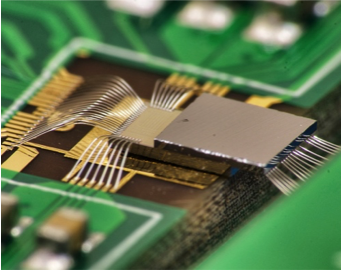
\includegraphics[width=.4\textwidth]{VertexDetector/CLICPIX/ccpdv3_clicpix.png}
    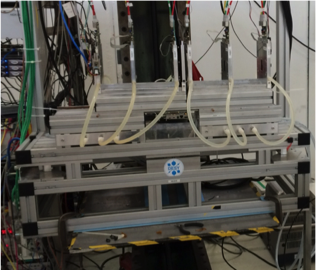
\includegraphics[width=.4\textwidth]{VertexDetector/CLICPIX/timepix3_telescope.png}
    \caption{Left:CCPDv3 + CLICPix. Right: Timepix3 in the AIDA telescope (CERN PS-T9)}
    \label{fig:VertexDetector:clicpix}
\end{figure}

\subsection{Recent Milestones}
A broad hardware R\&D program is in place, addressing the challenges for the CLIC
vertex detector in an integrated approach~\cite{1748-0221-10-03-C03025}. Recent achievements
in the sensor and readout domain include:
\begin{description}
\item[Hybrid pixel assemblies with ultra-thin planar sensors]
Planar pixel sensors with \SI{55}{\micro\meter} pitch and different thicknesses (\SIrange{50}{300}{\micro\meter})
were procured from different vendors and bump-bonded to Timepix~\cite{Llopart2007485} readout
ASICs (100 and \SI{700}{\micro\meter} thickness).
Slim-edge sensor designs are compared to designs
with active edges.
Preliminary beam-test results show very good efficiencies in both cases, extending beyond the
edge pixels~\cite{Redford:1966932}.
For \SI{50}{\micro\meter} sensor thickness and nominal readout parameters, the fraction of multi-pixel clusters
is approximately 20\%.
Single-point resolutions of approximately \SI{3}{\micro\meter} have been extracted
for clusters of two pixels using charge interpolation and taking into account
non-linear charge sharing.
\item[CLICpix demonstrator ASIC]
A CLICpix demonstrator chip has been produced in \SI{65}{nm} CMOS technology,
including a $64 \times 64$ pixel matrix and power-pulsing capability~\cite{Valerio:1507691}.
The pixel size is $\SI{25}{\micro\meter}\times\SI{25}{\micro\meter}$. Simultaneous
4-bit Time-Of-Arrival (ToA) and Time-Over-Threshold (ToT) measurements
are implemented in each pixel, allowing for a front-end time slicing
with approximately \SI{10}{ns} and for measuring the charge
to improve the position resolution through interpolation.
The full chip can be read out in less than
$\SI{800}{\upmu s}$ (for 10\% occupancy), using a \SI{320}{MHz} readout clock and zero suppression.
The
power consumption of the chip is dominated by the analog frontend
with a peak power corresponding to $\SI{2}{W/cm^2}$. The total average power
consumption can be reduced to a value below the target of $\SI{50}{mW/cm^2}$
by means of power gating for the analog part and clock gating for the digital part.
Readout tests have confirmed that the CLICpix demonstrator chip
is fully functional and the power consumption and performance are in agreement with
simulations~\cite{Valerio:1635171}.
Hybrid modules of CLICpix ASICs with planar slim-edge
sensor prototypes are currently in production.
\item[Capacitively coupled active HV-CMOS sensors]
Hybrid assemblies of CLICpix prototype chips with CCPDv3 active sensors
have been produced and tested.
The sensors are implemented in
a \SI{180}{nm} high-voltage CMOS process~\cite{Peric2013131}. A deep n-well above the low-resistivity
(few $\Omega$cm) p substrate
surrounds low-voltage p-wells and acts as the signal collecting electrode.
A nominal operation voltage of -\SI{60}{V} at the
n-well results in a depletion layer of approximately \SIrange{10}{20}{\micro\meter} in the p substrate.
 The fast drift signal collected in this
depletion layer passes through a two-stage transimpedance
amplifier in each pixel and the resulting voltage signal is capacitively coupled to the CLICpix
ASIC through a layer of glue a few microns thick.
Laboratory tests with radioactive sources show a good signal-to-noise performance for the
active sensor output. Preliminary test-beam results with CLICpix-CCPDv3 assemblies suggest a
detection efficiency of $>99\%$ for minimum ionising particles and a high fraction of
single-pixel clusters with a position resolution of
approximately \SI{7}{\micro\meter}, as expected for \SI{25}{\micro\meter} pixel pitch.
\item[Through Silicon Vias (TSV)]
A ``via last'' TSV process developed in collaboration with
CEA-LETI has demonstrated the feasibility of TSVs on functional
readout ASICs from the Medipix/Timepix chip family~\cite{6575630}.
The project uses Medipix3 readout wafers produced in \SI{130}{nm} CMOS
technology. The wafers are thinned to \SI{120}{\micro\meter} and the resulting vias
have a diameter of \SI{60}{\micro\meter}.
An ongoing  continuation of the TSV project aims at producing
TSVs in Timepix3 ASIC wafers thinned to \SI{50}{\micro\meter}.
\end{description}

\subsection{Engineering Challenges}
The detector performance requirements lead to challenging constraints
for the mechanical and electrical integration of the vertex-detector
components and its cooling system. An integrated approach is followed,
addressing several of the critical R\&D issues in these domains:
\begin{description}
\item[Power delivery and power pulsing] A low-mass power-pulsing and power-delivery
system optimised for the small duty cycle of the CLIC machine has been
developed~\cite{1748-0221-8-01-C01057}. Controlled current sources
deliver a low and almost constant current ($<\SI{300}{mA}$ per ladder)
into the vertex region through low-mass cables. The energy needed by the readout ASICs during the time of the collisions
and detector readout is stored locally in silicon capacitors. Low-dropout regulators provide the necessary stability
of the output voltage for the analog ($\Delta V\approx16$mV) and the digital part
($\Delta V\approx\SI{70}{mV}$) of the readout ASICs.
Prototypes have been tested successfully with dummy loads emulating the power consumption
of the 12 readout ASICs in a half ladder. The total contribution of the
powering infrastructure to the material budget of each barrel layer is
approximately 0.1\%X$_0$. It is expected to decrease to less than $0.05\%$X$_0$ with evolving silicon-capacitor technology.
\item[Cooling] Even with power pulsing a total power of approximately \SI{500}{W} will be dissipated in the vertex detectors alone. To limit the amount of material in the vertex-detector region, a cooling
system based on forced air flow is under development~\cite{DuarteRamos:1572989}. Finite-element Computational Fluid Dynamics (CFD) simulations show that air cooling is feasible. For a mass flow of \SI{20}{g/s}, the temperature increase
in the vertex detector is limited to approximately \SI{40}{\degreeCelsius}. The proposed cooling scheme is being
validated in thermal mockups. Preliminary results confirm the validity of the simulations.
\item[Mechanical supports] The low overall material budget leaves only about 0.05\%X$_0$ per
detection layer for mechanical supports. Prototypes based on Carbon-Fibre-Reinforced Polymers
(CFRP) are under study~\cite{VillarejoBermudez:1982810}. Bending-stiffness calculations have been validated in
finite-element simulations
and with bending tests. Measurements within an air-cooling mockup show
that the air-flow induced vibrations are at an acceptable level of approximately \SIrange{1}{2}{\micro\meter} RMS
amplitude for the direction perpendicular to the detector plane and at nominal flow conditions.
\item[Assembly and access scenarios]
Assembly and access scenarios for in-situ testing have been developed,
taking into account the constraints from the surrounding detector elements~\cite{VillarejoBermudez:1982810}.
Realistic cabling layouts are proposed and evaluated in terms of their impact on the
global and local material budget.
\end{description}

\subsection{Future Plans}
The technical development programme for the CLIC vertex detector aims at building
demonstration modules for the main components of the vertex detector system
in time for the next update of the European Strategy
for Particle Physics in 2018/19. To reach this medium-term goal, several technology prototypes
are under development.
Ultra-thin edgeless hybrid pixel assemblies with Timepix3 readout ASICs (including ASICs thinned to \SI{50}{\micro\meter}
and processed with TSVs) are currently in production.
The next version of the CLICpix demonstrator
ASIC (CLICpix2) is foreseen to be produced in the second half of 2015. It contains a larger
pixel matrix ($128\times 128$) and higher dynamic range (8-bit ToA and 5-bit ToT).
Slim-edge and edgeless sensors matching the $128\times 128$ CLICpix2 footprint have already been produced and an
improved version of the CCPD active HV-CMOS sensor will be submitted for production by the end of 2015.

\newpage
\thispagestyle{empty}
\newgeometry{margin=1.5cm} % modify this if you need even more space
\begin{landscape}
    \centering
    \begin{adjustbox}{max width=1.1\textwidth,totalheight=1\textheight}
\begin{tabularx}{2\textheight}{lXXXX}
    \toprule
    R\&D Technology & Participating Institutes & Description / Concept & Milestones & Future Activities \\
    \midrule
        ChronoPix &
        University of Oregon\newline Yale University\newline Sarnoff Corporation &
        ChronoPix is a monolithic CMOS pixelated sensor with the ability to record up to two time stamps per pixel during the bunch train. Hits are read out in the time between bunches. &
        April 2014: Device tests of prototype 2 inform the design of prototype 3 to be submitted to foundry &
        Prototype 3 was manufactured in September 2014. Tests have shown that problems revealed in prototype 2 were solved. \\
    \midrule
        CMOS MAPS &
        IPHC Strasbourg \newline DESY, Hamburg \newline University of Bristol \newline University of Frankfurt &
        The CMOS pixel sensor uses as a sensitive volume the \SIrange{10}{20}{\micro\meter} thin high-resistivity epitaxial Si-layer deposited on low resistivity substrate of commercial CMOS processed chips. The generated charge is kept in a thin epi-layer atop the low resistivity silicon bulk by potential wells that develop at the boundary and reaches an n-well collection diode by thermal diffusion. &
        2016 : production of CPS for the ALICE-ITS upgrade\newline
        2018/19 : production of CPS for the micro-vertex detector of the CBM experiment at FAIR/GSI\newline
        2018/19 : validation of light double-sided ladder concept combining highly granular sensors on one side with timestamping sensors on the other side\newline
        $< 2020$ : validation of power pulsing of double-sdied ladders inside a high magnetic field\newline
        2022/23 : finalisation of the R\&D on various CPS adapted to the different layers of a very high performance vertex detector at the ILC &
        Until 2018-2019: Development and production of CPS for the ALICE-ITS and CBM-MVD \newline Development of various CPS optimised for the different layers of a vertex detector at the ILC, with emphasis on bunch tagging \newline Development of low material double-sided ladders \\
    \midrule
        DEPFET &
        University of Barcelona, Spain \newline
        University of Bonn, Germany \newline
        Heidelberg University, Germany \newline
        Giessen University, Germany \newline
        University of G{\"o}ttingen \newline
        KIT Karlsruhe, Germany\newline
        IFJ PAN, Krakow, Poland \newline
        MPI Munich \newline
        MPG HLL Munich, Germany \newline
        Charles University, Prague, Czech Republic \newline
        IFIC, CSIC-UVEG, Valencia, Spain \newline
        DESY, Hamburg, Germany \newline
        IFCA, CSIC-UC, Santander, Spain &
        The DEPFET technology implements a single active element within the active pixel by integrating a p-MOS transistor in each pixel on the fully depleted, detector-grade bulk silicon. Additional n-implants near the transistor act as a trap for charge carriers created in the substrate (internal gate), so that they are collected beneath the transistor gate. &
        2014: Full-scale \SI{75}{\micro\meter} thin Belle II ladder in beam test at DESY &
        Development of die-attach technology \newline
        Full-scale test of all ASICs on ladder \newline
        Integration of read-out and steering ASICs on pixel sensor using flip-chip technique and microscopic solder ball bump-bonding \newline
        Production of Belle II vertex detector modules\newline
        Tests of the last version of the DHP chips \newline
        Engineering design for all-silicon module with petal geometry required for ILC\newline
        Detailed characterization of device response \newline
        Design of ancillary ASICs, taking full responsibility for future design cycles of the FE read-out chip, called Drain Current Digitizer \\
    \midrule
        FPCCD &
        KEK \newline
        Shinshu University \newline
        Tohoku University \newline
        JAXA, Japan Aerospace Exploration Agency &
        Fine Pixel CCD sensors have pixel sizes of \SI{5}{\micro\meter} and a fully depleted epitaxial layer with a thickness of \SI{15}{\micro\meter} &
        Fabrication of real size ($\SI{12.3}{mm} \times \SI{62.4}{mm}$) sensors with \SI{50}{\micro\meter} total thickness \newline
        Neutron irradiation of a small ($\SI{6}{mm} \times \SI{6}{mm}$) FPCCD sensor \newline
        Construction of a prototype cooling system and demonstration of cooling between \SI{-40}{\degreeCelsius} and \SI{+15}{\degreeCelsius} &
        Characterization of FPCCD sensors including beam tests and radiation damage studies \newline
        Development of FPCCD sensors with a pixel size of \SI{5}{\micro\meter} \newline
        Construction of prototype ladders for the inner layers of a vertex detector \newline
        Development of readout electronics downstream of ASICs \newline
        Development of larger FPCCD sensors and prototype ladders for outer layers \newline
        Development of readout electronics with a small footprint \newline
        Construction of a real size engineering prototype and cooling test \\
    \midrule
        3D Pixels &
        Brown University \newline
        Cornell University \newline
        Fermilab \newline
        Northern Illinois University \newline
        SLAC \newline
        University of Illinois Chicago &
        3D technology allows very fine pitch (\SI{4}{\micro\meter}) integration of sensors with multiple layers of electronics, allows interconnection oto both the top and bottom of devices, and provides techniques for low mass, thinned devices. &
        Completed multi-year effort to demonstrate commercial 3D technology, consisting of \SI{0.13}{\milli\meter} CMOS interconnected with Direct Oxide bonding technology and access using TSV. \newline
        Received readout wafers with thickness of \SI{25}{\micro\meter}, processed with TSV and DBI to connect to 3D electronics \newline
        Currently working on active edge demonstrator devices &
        Complete the 3D active edge project \newline
        Apply concepts to x-ray imaging devices \newline
        Re-start ILC developments pending renewed funding \\
    \midrule
        SOI &
        KEK\newline
        University of Tsukuba \newline
        Tohoku University \newline
        Osaka University &
        In the Silicon-On-Insulator (SOI) technology the sensing and processing functionalities are separated in different layers; the sensing is provided by a high-resistive substrate connected through an insulating layer with the processing layer. &
        &
        Sep 2014: Complete architecture study for the ILC pixel detector \newline
        Mar 2015: Design and fabrication of first test chip for the ILC \newline
        Dec 2015: Beam test of the chip \\
    \midrule
        CLICPix
        &
        Cambridge University\newline
        CERN\newline
        University of Geneva\newline
        Karlsruhe Institute of Technology (KIT)\newline
        University of Liverpool\newline
        SLAC\newline
        Institute of Space Science Bucharest\newline
        Spanish Network for Linear Colliders
        &
        Hybrid pixel-detector technology comprising fast, low-power and small-pitch readout.
        ASICs implemented in \SI{65}{nm} CMOS technology (CLICpix) coupled to ultra-thin planar
        or active HV-CMOS sensors via low-mass interconnects.
        &
        Beam tests of prototype assemblies with ultra-thin sensors (\SIrange{50}{300}{\micro\meter})\newline
        CLICpix demonstrator ASIC in \SI{65}{nm} technology\newline
        Beam tests of assemblies with capacitive coupling between CCPDv3 HV-CMOS active sensors
        and CLICpix ASICs\newline
        Power-pulsing demonstrator with dummy loads\newline
        Prototypes of carbon-fibre ladder supports\newline
        Full-scale thermal mockup of the CLIC vertex-detector region
        &
        Demonstration modules for all major components
        in time for the next update of the European Strategy
        for Particle Physics in 2018/19
        \\
    \bottomrule
\end{tabularx}
\end{adjustbox}
\end{landscape}
\restoregeometry

% \subsubsection{The AHCAL in ILD and SiD}
The AHCAL prototype development follows the ILD detector design, and the performance studies, which guide the R\&D, are performed in the ILD concept. The detailed AHCAL simulation, as implemented in the ILD, has been shown to reproduce test beam results, and the components realized in prototypes are represented in the engineering model of ILD. There is close consultation between CALICE and the concepts on prioritizing the R\&D which is still needed on the way to a realistic technical proposal.

The AHCAL also constitutes an option for the hadronic calorimeter of the SiD concept. It is straightforward to transfer the technical and integration solutions developed in the ILD context to SiD, because the basic geometry and the routing of signals are very similar. However, the detailed integration of the AHCAL in the engineering model and in the simulation is not yet as advanced as for ILD. For example, the optimization of the cell size still needs to be done for the SiD case with its smaller detector radius and the more finely segmented ECAL. Steps are being taken on the software side, but the engineering support is sub-critical. There is regular exchange between CALICE and SiD on these issues, both the conceptual as well as on the technical level.

\newpage
\chapter{Silicon Trackers}
\section{Motivation and Constraints for Silicon Tracking at Linear Colliders}

Accurate matching between the track and the shower components of charged particles is one of the cornerstones of particle flow algorithms. Detector concepts at Linear Colliders therefore aim to measure the tracks of charged particles with the utmost precision to follow them from the point of creation to where they enter the calorimeters.

The concept of Silicon tracking uses several measurements with small errors to reconstruct the helix of charged particles in a magnetic field. The CMS experiment at the LHC is demonstrating that tracking with a precision required by the particle flow paradigm can be successful.

Silicon tracking detectors at Linear Colliders are faced with challenging requirements on the material budget. On the one hand, this goes along with thinner sensors and therefore lower signal-to-noise ratios, on the other hand, this leads to requirements on low power ASICs to allow passive cooling. In addition, silicon tracking allows the precise determination of the time of the hit, which significantly improves pattern recognition in the presence of background from machine-related processes.


\section{Long-Ladder and Charge Division Tracking R\&D}
Most recent update: 2015-08-09 \\
Contact person: Bruce Schumm (email: baschumm@ucsc.edu)
\subsection{Introduction}

The SiD consortium has pursued microstrip R\&D in two directions that might provide attractive
alternatives to the SiD baseline: the exploration of the long-ladder limit for precision
microstrip tracking, and the exploration of the use of ``charge division'' -- reading out
resistive electrodes from both ends --
to glean information about the longitudinal position of the track
along the length of the sensor.

Two activities have been undertaken for the exploration of the long-ladder limit:
the development of an optimized, time-over-threshold readout ASIC (the LSTFE chip)
and a lab-bench study of the noise limitations associated with reading out long,
thin electrodes.
The possibility of using charge division to determine the longitudinal
coordinate of deposited charge with sub-centimeter precision was explored
using a mock electrode network read out with an optimized amplification and
shaping chain. Milestones have been achieved in all three areas.

\subsection{Recent Milestones}

The properties of this Long Shaping-Time Front End (LSTFE) microstrip readout ASIC have
been optimized for the readout of long ladders of silicon strip sensors that are motivated
by the need for precise low-mass central tracking for a Linear Collider Detector. With a
small and straightforward change to the shaping properties of the ASIC, it could be re-optimized
for use for the short strips and high occupancy that would be expected for ILC forward-tracking applications.
The LSTFE features optimized initial-amplification characteristics
and shaping time to reduce voltage-referenced readout noise, as appropriate for narrow-strip, long-ladder
applications. Unique to the LSTFE design, however, is the use of time-over-threshold readout to estimate the
analog pulse-height generated by subatomic particles passing through. A pulse-development and readout simulation developed
for the purpose of the designing the LSTFE suggests that the intrinsic statistical fluctuations of the
charge-deposition process in \SI{300}{\micro\meter} of silicon obviate the need for a precise measurement
of deposited charge. A simulation of the centroid-finding (position-resolution) uncertainty provided by
time-over-threshold readout showed little degradation relative to that provided by an exact measurement of
deposited charge.

On the other hand, there are several advantages offered by the use of time-over-threshold readout. It is very simple
to implement within a digital back-end to the LSTFE's analog front end (the implementation would be on the same chip
as the front-end readout), requiring only a measurement of the number of clock counts that the given channel is over
threshold, and then the assembly and transmission of a
single data word containing the time of the upward transition, the time over threshold after the transition, and the
channel number. This happens in real time and is driven immediately off the chip into the DAQ, eliminating the need
for buffering and ADC conversion. In particular, there is no limit to the rate at which particles can be detected
other than the return-to-baseline of the analog signal, and so the data-accumulation rate capability of the device
is very high. In addition, for forward tracking, for which short strips are envisioned, the shaping time can be
shortened significantly. This will further improve the rate capability of the LSTFE readout, making it an excellent
choice for the high-occupancy forward region.
% Figure~\ref{fig:Tracker:SCIPP:LSTFE} shows the fractional pulse-height uncertainty versus
% injected charge achieved with the LSTFE front-end ASIC.
%
% \begin{figure}
% 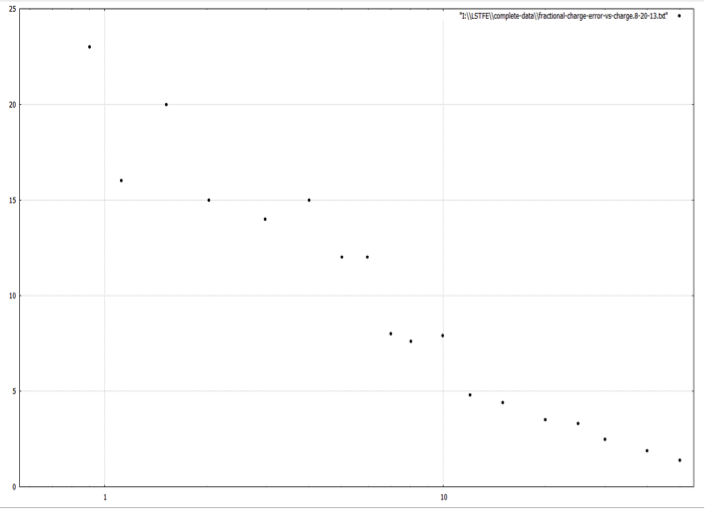
\includegraphics{Tracker/SCIPPTracking/SCIPPTracking}
% \caption{Fractional pulse-height uncertainty (percent) versus injected charge (fC) for the LSTFE front-end ASIC.}
% \label{fig:Tracker:SCIPP:LSTFE}
% \end{figure}

The possibility of obtaining a longitudinal coordinate from silicon
microstrip sensors has been explored~\cite{Carman2011118}, making use of the
implant as a resistive electrode, with no overlain metallic electrode. An mock resistive
microstrip-implant electrode network was constructed on a PC board out of discrete resistors and capacitors
which was read out on both ends by an amplifying and shaping chain that was optimized to give the greatest
precision in the longitudinal position of the charge deposition on the implant. For a \SI{10}{cm}-long sensor,
a longitudinal resolution of \SI{6}{mm} was observed, achieving the resolution needed to aid in tracking
reconstruction in dense jet environments. Finally, sources of readout noise were measured and modeled
for sensors in the long, thin strip electrode limit~\cite{Collier2013127}. The readout noise observed
with the LSTFE ASIC was measured as a function of the length of a daisy-chained ladder of sensors,
and the results modeled with a SPICE simulation. It was found that network effects due to the
distributed resistance and capacitance of the electrode provide significant
mitigation of the readout noise relative to the assumption of single, lumped elements. It
was also found that reading out the ladder at its center rather than from one end provided
further noise suppression. Attaching this noise model to the pulse-development simulation
developed for the LSTFE design suggested that ladders of as much as \SI{75}{cm} long could be
made operation with end readout. Ladders approaching \SI{1}{m} in length could be operated with center readout.

\subsection{Engineering Challenges}

The primary remaining engineering challenges are the implementation of LSTFE power-cycling with a $\approx 1\%$
duty cycle, and the transfer of the digital back-end processing of the LSTFE information from
an off-chip FPGA directly onto the ASIC.

\subsection{Future Plans}

Because of this work, the possibility of a tracker making use of long ladders of silicon
microstrip sensors, or shorter strips with time-over-threshold readout in the forward
region, remains an option for the SiD detector. However, at this time resources are
being directed towards the modular KPiX design.



References
\begin{itemize}
\item \fullcite{Carman2011118}
\item \fullcite{Collier2013127}
\end{itemize}

\section{Resistive charge-division on thinned micro-strips sensors with low signal amplification}
Most recent update: 2015-11-15\\
Contact person: Ivan Vila Alvarez (email: ivan.vila@csic.es)
\subsection{Introduction and Motivation}

In the context of the ILC, the relatively low occupancy environment and the power pulsing operation of the front-end electronics provide an opportunity for the implementation of ultra-lightweight silicon-based tracking systems where the dominant contribution to the material budget in the fiducial volume comes from the sensors. Reducing the material budget has a major impact on the hit position resolution and hence the momentum resolution of the tracker system; therefore, we have pursued during the last three years an RD program for the development of very thin micro-strips sensors able to provide two dimensional information of the hit position.

The ultimate goal of this R\&D is the development of a micro-strip sensor which combines signal amplification --- allowing the thinning of the sensor’s substrate --- and resistive electrodes --- allowing the implementation of the charge-division method for the determination of the hit position along the strip direction. In a first phase, we are aiming to demonstrate the feasibility of each of the above mentioned features independently and, in a second phase, to integrate both technological solutions into the same micro-strip sensor; the thinning of the sensor will done using the anisotropic wet etching (TMAH process) used for the DEPFET fabrication \ref{sec:DEPFET}.

\subsection{Recent Developments and Milestones}

The use of the charge-division method in long micro-strip sensors, with a length of several tens of centimeters, was proposed as a possible tracking technology for the International Linear Collider detector concepts a few years ago~\cite{Carman:2011zz}. More recently, we have demonstrated \cite{2012JInst...7.2005B,Bassignana2013186,Curras:ICHEP2014} the feasibility of the charge division concept on fully fledged micro-strip sensor with resistive electrodes made of poly-cristalline silicon achieving a spatial resolution along the strip direction of about 7\% the strip length. One of the limitations of this technology is the attenuation of the signal along the resistive electrode; additionally, the position resolution along the strip is proportional to the signal--to--noise ratio. Therefore, to maintain or even increase the SNR without increasing the sensor substrate thickness we proposed the integration of signal amplification structures in the sensor itself. The Low Gain Avalanche Detector (LGAD) technology appears as a well suited technique for achieving the signal amplification.
LGAD devices engineered as reach-trough avalanche detectors with a moderate gain where initially proposed and developed for timing application [Pellegrini 2014], the moderate signal amplification ensured that a relatively standard front-end readout electronics could be employed. As a spin-off of this original aim, we introduced the i-LGAD micro-strip concept for tracking, a LGAD device implemented in a p-type substrate where the ohmic electrode is strip-wise segmented; this design favors the uniform signal amplification over the sensors active volume overcoming the non-uniform gain in LGAD micro-strips sensors with a strip-wise segmented amplification layer that we recently characterized~\cite{Pellegrini:Hiroshima2015,Vila:LCWS2015}.
The former R\&D line is complemented with the development of a dedicated ASIC using a \SI{180}{nm} AMS fabrication process which integrates a charge amplifier with long shaping time and time stamping functionalities; finally, we completed the study and testing of several pulsed power system topologies based on super-capacitors.

\subsection{Engineering Challenges}
Concerning the component aspects, the main challenges are to complete to proof-of-concept of the thinned micro-strips with charge amplification and resistive charge-division in a implementation suitable for the LC tracking needs, namely:  proof the i-LGAD concept, integrating amplification and charge division, thinning of sensors substrate, large area sensors, manufacturing long ladder by daisy chaining of the sensors. Concerning the read out ASIC, the main challenge will be the design of the front-end with the required functionalities while keeping the power dissipation low enough.
System wise, the main challenge is the design of an air-based cooling system and its integration on the CFRP supporting structure such that the material budget of the system remains acceptable from the point of view of it tracking performance.

\subsection{Future detector R\&D}
During the next two years we will focus our activities on the testing of the i-LGAD devices and, if the results were positive, the integration of the low gain amplification and manufacturing of large area sensors ($\SI{100}{cm^2}$). Concerning the front-end electronics, the main goal will be to complete a few channel demonstrator integrating the long shaping time amplifier and power pulsing. A real scale thermo-mechanical mockup is of the FTD sub-detector at ILD is currently under construction to assess different air forced cooling options.

\newcommand{\LYCORIS}{{\textsc{Lycoris}}\xspace}
\newcommand{\DESYII}{{\mbox{DESY II}}\xspace}
\newcommand{\DIITBF}{{\DESYII Test Beam Facility}\xspace}
\newcommand{\SID}{{SiD}\xspace}
\newcommand{\KPIX}{{KPiX}\xspace}


\section{\KPIX Silicon Tracking}
Most recent update: 2020-05-1135 \\
Contact person: Marty Breidenbach (email: mib@slac.stanford.edu)\\
Contact person: Marcel Stanitzki (email: marcel.stanitzki@desy.de)\\
Contact person: Mengqing Wu (email: mengqing.wu@desy.de)\\




\subsection{Introduction}
The baseline design of the \SID Tracker as presented in the ILC TDR~\cite{Behnke:2013lya} is based on an all-silicon approach.
The main tracker technology of choice is silicon strip sensors arrayed in five nested cylinders in the central
region and four disks following a conical surface with an angle of 5~degrees with respect to the normal to the 
beam line in each of the end regions. The geometry of the end-caps minimizes the material budget to enhance 
forward tracking. The basic building block is a module consisting of a single-sided silicon sensor, two \KPIX readout ASICS and a small Kapton-flex cable
for power delivery and signal distribution.
The sensors have a size of approximately 10 $\times$ 10 cm$^2$, a strip pitch of \SI{25}{\micro\meter} and a readout pitch of \SI{50}{\micro\meter}.
The end-caps utilizes two modules back-to-back for small angle stereo measurements. 
Each sensor is read out by two \KPIX ASICS and connected to the DAQ and the power-supply system using a small Kapton-flex cable. This hybrid-less design 
further reduces the material budget leading two a very light-weight tracking system. A drawing of a Tracker module is shown in 
Figure~\ref{fig:SiliconTrackin:KPiX:module}.


\begin{figure}
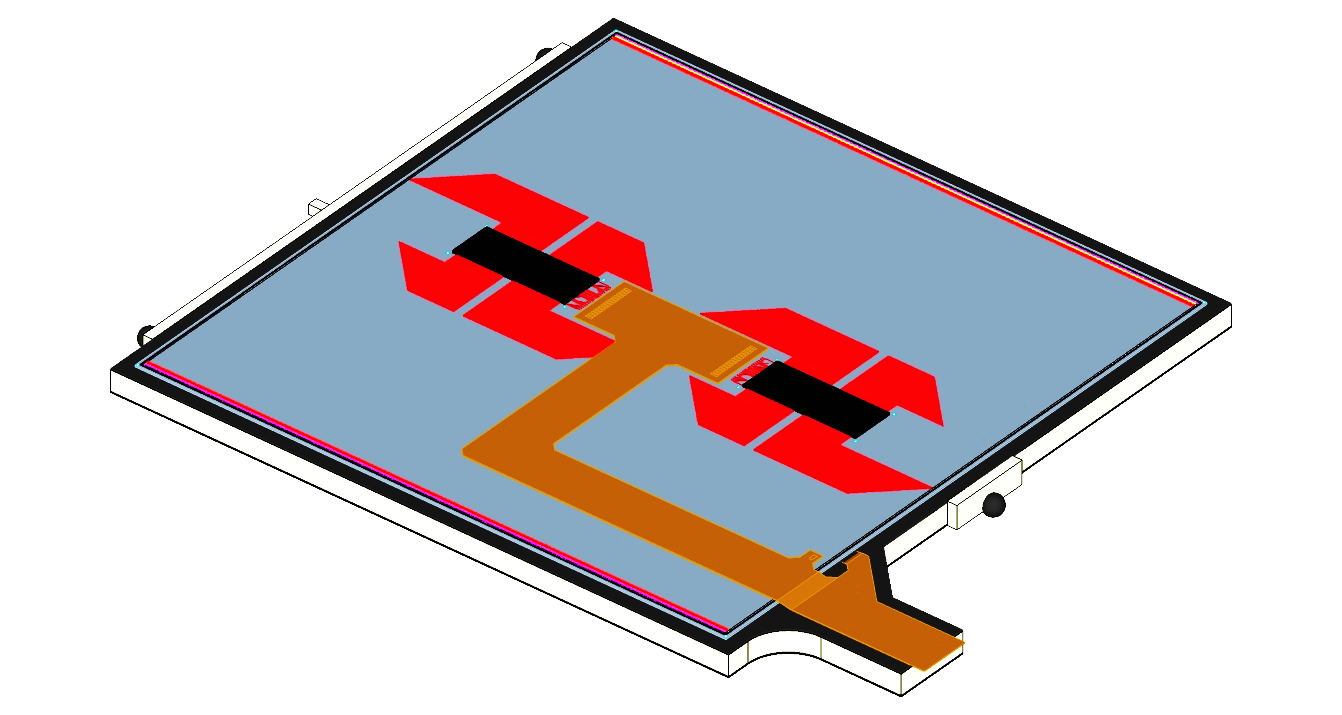
\includegraphics[width=0.49\textwidth]{Tracker/KPIX/Tracker_Module_SiD_Drawing.png}
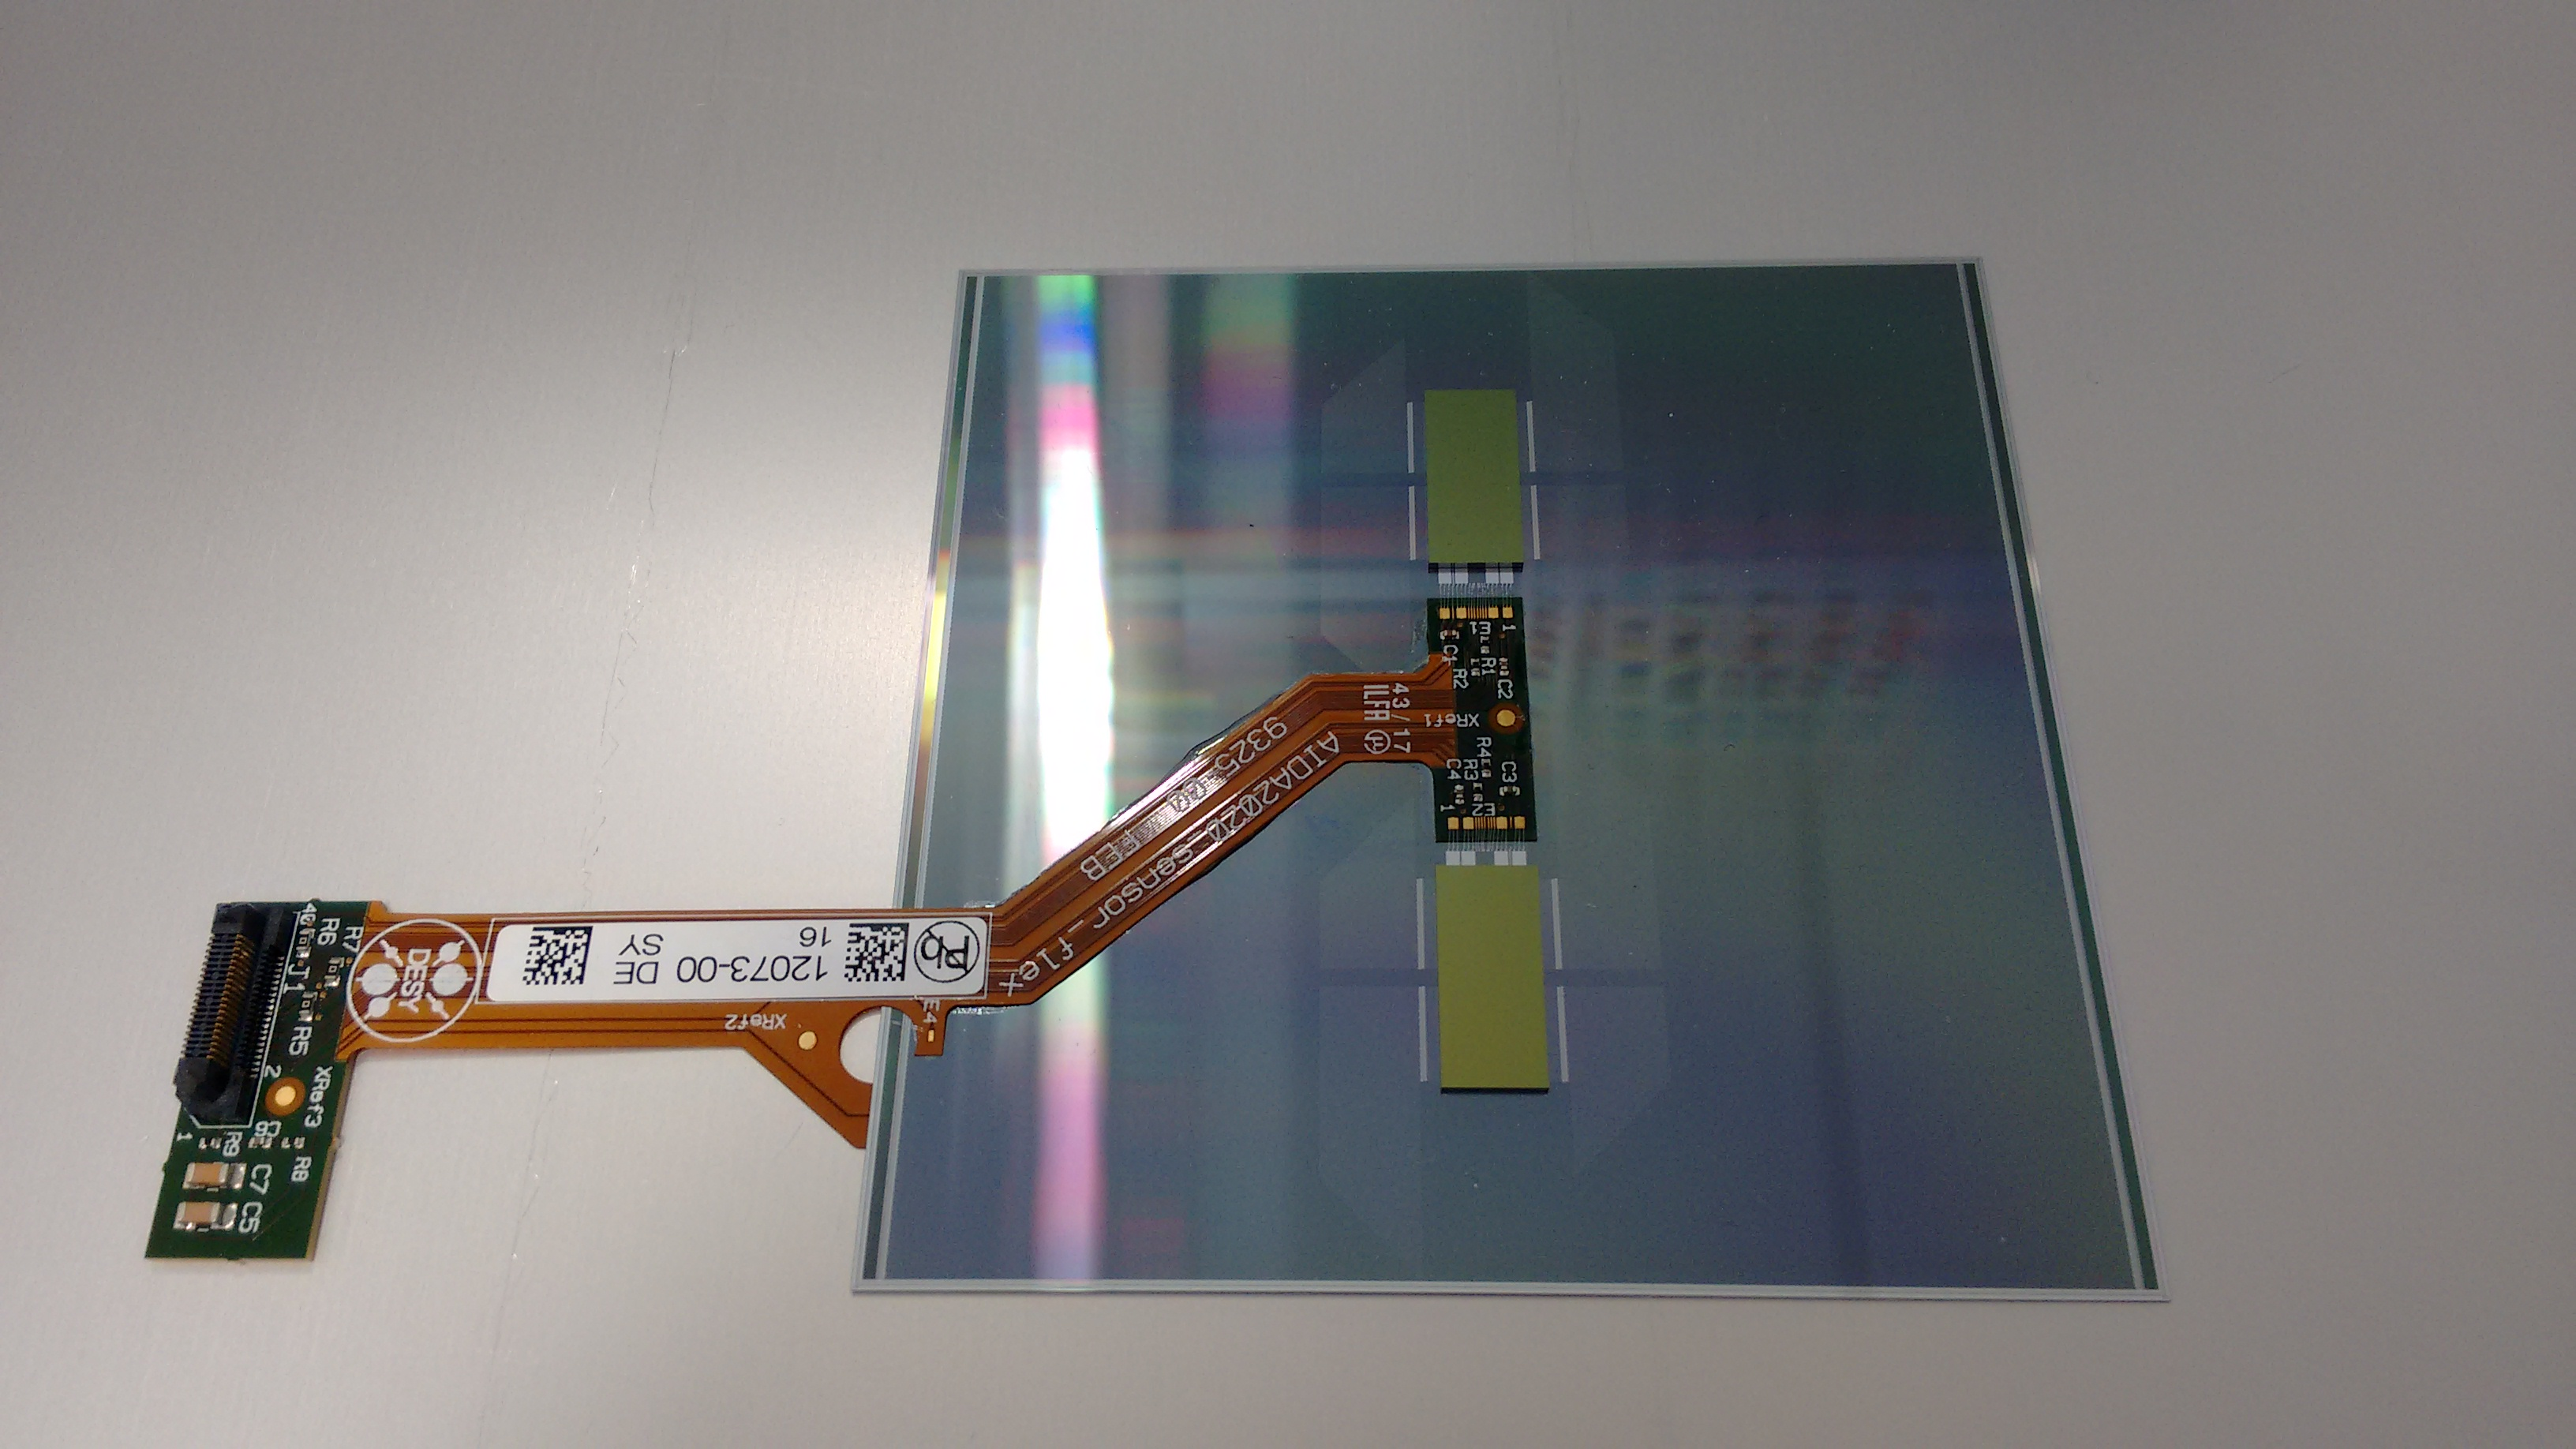
\includegraphics[width=0.49\textwidth]{Tracker/KPIX/Tracker_Module_SiD_Photo.jpg}
\caption{This \SID Tracker Module as foreseen for the baseline \SID Tracker\cite{Behnke:2013lya} with the two \KPIX ASICS and the Kapton-Flex cable 
and a first prototype sensor fully completely assembled at DESY}
\label{fig:SiliconTrackin:KPiX:module}
\end{figure}

The \KPIX ASIC~\cite{6551433}is a 1024 channel ``System on a Chip'' intended for bump bonding 
to large area silicon sensors, enabling low multiple scattering silicon-strip 
tracking and high density Particle Flow calorimetry for \SID at the ILC. 
Each channel consists of a dynamically switchable gain charge amplifier; 
shaping; threshold discrimination; and four sample and hold 
capacitors and four timing registers. The chip permits four  separate measurements of 
amplitude and time of threshold crossing during each train, and amplitude 
digitization and readout during the inter-train period. The dynamic range is from 
sub minimum ionizing particle (MIP) (in \SI{320}{\micro\meter} silicon) to more 
than 2000 MIP. \KPIX also has a calibration system for each channel, servos for 
leakage compensation, ``DC'' reset for asynchronous operation for testing with 
cosmic rays, and polarity inversion for use with GEMs and similar detectors. The 
noise floor is about \SI{0.15}{fC} ($\simeq$ 1000 electrons), and the maximum 
signal is \SI{10}{pC} (utilizing the dynamic range switching). The full dynamic 
range corresponds to 17 bits. \KPIX was manufactured using a \SI{250}{\nano\meter} process at TSMC.
In addition to its use in the \SID tracking system  \KPIX is also the proposed readout ASIC  for the \SID Silicon-
tungsten sampling electromagnetic calorimeter (see Section~\ref{sec:Calorimeter:SiliconTungstenSiD}).



\subsection{Recent Milestones}
ILC related R\&D in the US has been largely unfunded and small efforts are being kept alive. The \KPIX R\&D is such an example of necessary work for \SID.
In the last three years, the R\&D for \KPIX Silicon Tracker has been used to design and build a large-area silicon-strip 
telescope -- called \LYCORIS -- for the \DIITBF~\cite{desytb2018} as part of the Horizon2020-funded AIDA2020~\cite{AIDA2020} project.
\LYCORIS did require both the coverage of a large area (10 $\times$ \SI{10}{\centi\meter}

Based on the experiences with the first set of sensors, the second generation of sensors was produced by Hamamatsu 
using Au pads for the \KPIX bump-bonds and with a thicker oxide-layer. This was necessary, because the first generation Tracker sensor could not be 
wire-bonded to its (very thin) cable, which was unexpected. It was discovered, that the sensor oxide layer was not strong enough 
to allow wire bonding without damaging the sensor itself.

These changes have proven successful and these sensors were successfully bump-bonded to two \KPIX ASICS and wire-bonded to their Kapton-flex pigtail 
(See Figure~\ref{fig:SiliconTrackin:KPiX:module}. 

The \LYCORIS telescope has been successfully assembled and operated at DESY. 

some plots here ...

The key points demonstrated by \LYCORIS include operating a system of six modules with twelve \KPIX together, 
a hit resolution of about \SI{7}{\micro\meter} even if only second strip is read out, the 
validation of the power-pulsing design.



\subsection{Engineering Challenges}
At this time, \KPIX is seen as the baseline readout system for both the \SID tracker and electromagnetic calorimeter. 

The \LYCORIS telescope has demonstrated that the hybrid-less approach works well, the issues both with wire-bonding and 
bump-boding have been addressed and the modules can be made with a high yield - albeit this is based on small statistics.
In terms of the \SID tracker the next steps involve all the system issues of large-area tracker, e.g. cooling, services and mechanical stability. 
The alignment of such a system also needs further studied and the potential of FSI-based alignment systems need to be shown. 

There remain however some noise issues with the current \KPIX design, particular in the so-called high-gain mode, 
which is important for the tracker. This is currently under detailed study and the results will inform a possible 
next-generation \KPIX. Another concern is that the current design of \KPIX has dead time after a pixel 
has accepted a trigger. Only the triggered pixel is affected; all the other 
pixels are available for signals. This dead time is different from the usual 
notion of data acquisition dead time where the entire detector is unavailable, 
but the correction to the luminosity integral is easy. Finally, the buffer 
requirement (four in the current version of \KPIX) has being re-evaluated in \SID  
simulations using the latest beam background estimates. The conclusions are, that particularly for 
the end-caps a move to 8 or more buffers is beneficial. A possible new architecture for \KPIX is in early stages of  evaluation.


\subsection{Future Plans}
\LYCORIS is now going to be used at the \DIITBF and is made available to all users. This will yield essential long-term operational experience and 
advance the experience with the hybrid-less modules.  

For \KPIX a new architecture with little (or no) deadtime will be evaluated. A decision will be made to develop this new architecture or incrementally 
improve the existing design. At the same time, \SID will discuss, whether moving to a fully monolithic tracker sensor is beneficial given the past technological 
developments and the timescales involved.
	
Assuming positive developments with Japan are announced soon, we expect the financial support to improve globally. It should be noted that
an important effect of the withdrawal of support is the slow decay of expertise, with many collaborators having to work on other projects. We expect, that 
a positive statement will lead to resurgence of interest in this technology.

	
\subsection{References}

\begin{itemize}
\item \fullcite{lycoris-D15.2}
\item \fullcite{Kraemer:2018qzh}
\item \fullcite{Kraemer:2019xku}
\item \fullcite{Wu:2020jdk}
\item \fullcite{Kraemer2020_jinst}
\end{itemize}

\thispagestyle{empty}
\newgeometry{margin=2cm} % modify this if you need even more space
\begin{landscape}
    \centering
    \begin{adjustbox}{max width=\textwidth,max totalheight=\textheight}
    \begin{tabularx}{\textwidth}{lXXXX}
    \toprule
    R\&D Technology & Partici\-pating Institutes & De\-scrip\-tion / Concept & Milestones & Future Activities \\
    \midrule
    Long-Ladder & UC Santa Cruz & Long silicon ladder design \newline ``charge division'' & Test beam at SLAC \newline & write a note\\
    \midrule
    Micro-strips & CSIC &  &  & \\
    \midrule
    \KPIX Silicon Tracking & DESY\newline SLAC\newline U Oregon  & hybrid-less \newline silicon-tracker \newline design &  Publication & Design Review  \\
    \bottomrule
\end{tabularx}
\end{adjustbox}
\end{landscape}
\restoregeometry

\chapter{Gaseous Trackers}
% LCTPC collaboration spokesperson: Jochen Kaminski (email : kaminski@physik.uni-bonn.de)
\section{Motivation and Constraints for Gaseous Tracking at Linear Colliders}

Gaseous tracking devices have been extremely successful in providing precision pattern recognition for collider experiments. They provide hundreds of measurements on a single track, with an extremely low material budget in the central region of the detector. This results in excellent pattern recognition and hence tracking efficiency.

The continuous measurements of charged particle tracks also affords particle identification capabilities, which has the possibility to improve the jet energy resolution and flavor tagging capability of the experiment. These are two essential advantages for experiments at a linear collider.

The main challenges for the design of a large Time Projection Chamber (TPC) at a linear collider detector are related to the high magnetic field of the solenoid, in which the detector has to operate. For accurate measurements of the momenta of charged particles, the field map has to be known with high precision. While the event rate of an ILC detector can easily be accommodated by current TPC readout technology, R\&D to mitigate the effects of secondary processes from bunch -- bunch interactions is ongoing.

%%%%%%%%%%%%%%%%%%%%%%%%%%%%%%%%%%%%%%%%%
% Main part
%%%%%%%%%%%%%%%%%%%%%%%%%%%%%%%%%%%%%%%%%
\section{LCTPC Overview}
Detectors for a high energy linear electron positron collider have been discussed since the early 1990's. For the main tracking a TPC was proposed early on.
The advantages of a TPC are its ability to detect track elements in 3 dimensions while introducing very small amounts of dead material. A potential disadvantage could be the appearance of distortions due to $E \times B$ effects in the drift region, originating from possibly inhomogeneous magnetic or electric fields, which could be a consequence of the construction or from space-charge build-up as a result of ion back-flow.

In 1996, the first Linear Collider detector conceptual report \cite{Settles:1997wj} considered the possibility to read out the end-cap chambers with MSGC, Micromegas and GEMs. Several advantages of the MPGDs were recognized immediately: the ion back-flow could be very limited by a suitable choice of the field configuration, and the $E \times B$ effects present close to the wires of a MWPC are very limited in the case of the microscopic structure of a MPGD. However it was also recognized that, to profit from the
excellent resolution allowed by a limited diffusion and a very localized avalanche, either sufficiently small pads would be needed, to share the charge among several pads, or a mechanism for spreading the avalanche was needed. Without such a sharing, the only information obtained would have been which pad received the charge, and the hit position would have a flat probability over the pad width, limiting the resolution along a pad row to $p/\sqrt{12}$, $p$ being the pitch over a pad row. It was also
understood that for a multi-stage GEM, the amount of natural spreading by diffusion in the gas amplification device itself, about $\SI{300}{\micro m}$ r.m.s., was sufficient to obtain enough charge spreading with $\sim\SI{1}{mm}$ wide pads. For Micromegas, where the avalanche has typically a $\SI{15}{\micro m}$ r.m.s., an
additional charge-spreading mechanism was necessary, even for \SI{1}{mm} pads. Such a method was introduced by the Carleton group, using a superposition of an insulator and a resistive cover. This arrangement provides a continuous Resistor-Capacitance (RC) network over the surface which spreads the charge around the avalanche. The induced
signal is measured, shaped and digitized by the electronics connected to each pad. Note that this technique is applicable also to GEMs and allows pad widths of 2, 3 or more mm.

On the electronics side, a higher density readout might be necessary, to mitigate the background at small radius and to improve two-track separation where the track density is highest, as well as the fake hit density. This can be done by switching to the \SI{65}{nm} technology for the
chip design. Though the present consumption is rather moderate (\SI{15}{mW/channel}), a suitable power-pulsing operation should be adapted.
Early estimates show that such a system can be designed, but requires a careful balance between power saving and increased complexity.

At the beginning of the years 2000, several small prototypes were built in Aachen, Amsterdam, Saclay-Orsay with a Berkeley electronics, DESY, Munich, Karlsruhe, Carleton, Victoria, Saga, KEK, Tsinghua, to study various aspects of the GEM and Micromegas technology. Ion feed-back was studied, resolution was measured in various prototypes, and the possible gases were studied. The fundamental proof was made that a TPC with MPGD readout can be operated stably, and can reach intrinsically the anticipated resolutions.

Then, in 2004, part of the nascent collaboration gathered around a \SI{5}{GeV} pion beam and cosmic-ray tests at KEK. The detector was immersed in a \SI{1}{T} magnetic field from a permanent-current superconducting magnet. The \SI{25}{cm} drift field cage was designed in Munich and electronics was recuperated from ALEPH. Several endplates were adapted to this cage with wires, Micromegas (without resistive foil) and GEM technologies. In 2006 the Carleton \SI{16}{cm} drift length prototype with a Micromegas resistive foil took data simultaneously with the Munich prototype.

At the same time other developments took place in other institutes. Noteworthy was the use of 2 parallel laser beams in Victoria and later at DESY to study 2-track separation. This study showed that a separation of two tracks was possible down to 1 pad size distance between the laser beams.

Several groups carried out tests in a \SI{5}{T} magnet at DESY in the years 2003-2007. The operation in such high fields could be established for both Micromegas and for GEMs, and the extrapolation of the resolutions previously measured at lower fields could be demonstrated.

The next step then was the construction and operation of a common large prototype. The European Union - funded project EUDET allowed a facility to be built at DESY, with a 1T SC magnet offered by KEK, a field cage designed at DESY, an endplate brought by Cornell, a cosmic trigger with SiPMs built by Saclay, a beam trigger from Nikhef, a gas system from DESY and Rostock, high density readout electronics by Saclay and Lund, etc., and the B-field map was measured by CERN.

The endplate has 7 openings to receive up to 7 identical modules. The ``keystone'' shape of the modules is chosen to be as close as possible to the anticipated real configuration of a disc paved by concentric rows of modules. Data taking started in 2008 in the fixed magnet. At this time, to shoot the beam at a given z position along the drift axis was possible only by sliding the TPC in the  magnet; this way, the large drift distances could only be obtained by taking the TPC in a very inhomogeneous field. This was solved the following years by the installation of a moving stage allowing horizontal and vertical translations, as well as rotations in the horizontal plane. Rotation of the TPC around the  magnet axis could be performed by hand.

Since then beam tests took place nearly every year, alternating between GEMs from Japan, Micromegas, GEMs from DESY, and pixels.
The pixel read out is based on a GridPix detector, where close to a pixel ASIC a grid is put
by wafer post-processing techniques. The device was invented around 2000 and on the
basis of several generations of chips (Medipix2, Timepix and Timepix3) detectors of different
size and complexity were constructed and tested. The pixel read out is since 2020 one of the
baseline options for a TPC.
    
\section{GEM based Readout}
\label{chap:TPC_sec:standard_gems}

Gas Electron Multipliers (GEMs) \cite{Sauli1997531} have been invented in the mid 90's. They consist of a thin polyamide foil, covered with Copper on both sides. Holes are produced into the foil on a regular pattern. Typical dimensions are a hole pitch of \SI{140}{\micro m} and a hole diameter of \SI{70}{\micro m}. If an electric field is applied between the two sides of the foil, high fields form inside the holes, and provide avalanche gas amplification. Since the high fields are constrained inside the holes, many of the high-voltage problems connected to traditional wire based chambers are not relevant. GEM foils can be stacked to provide tailored gas amplification. During the years a number of different types of GEM foils have been developed. They differ for example in the cross section of the holes, in the material of the foil, and in the pitch and hole sizes. For application in the ILC TPC currently two main options are being pursued. The first one is based on a GEM where a laser is used to ``drill'' each hole.
The resulting holes are
strictly cylindrical. The second option is based on a chemical etching process. The resulting holes have a double conical shape.

In addition to the different types of GEM foils two different schemes to build readout modules for the TPC are investigated. Scheme one (called module type A in the following) relies on a sturdy aluminum frame where the GEM foils are stretched between the bottom and the top of the readout module. This scheme allows to build a module which has essentially no dead area on the side of the module, but where some dead space is needed on the top and the bottom. The second option (called module type B in the following) relies on an assembly of a stiff but thin ceramic frame which when glued to the GEM provides a self-supporting stiff assembly. The width of the frame is around one millimeter, so that in this approach a small dead area is present all around the module. Both approaches allow the stacking of GEM foils, and both are compatible with the installation of a gating GEM on top.

\subsection{Module Type A, ``Asian Module''}
\label{chap:TPC_sec:asian_gems}
Most recent update: 2016-03-28\\
Contact person: Akira Sugiyama(email: sugiyama@cc.saga-u.ac.jp)\\

The Asian modules use GEM stacks as a gas amplification stage and are optimised to reduce the insensitive area
on the sides of the modules which point towards the detector center.
A module can be seen in figure \ref{fig_Fig1asiangempicture}.

\begin{figure}[!htb]
  \centering
  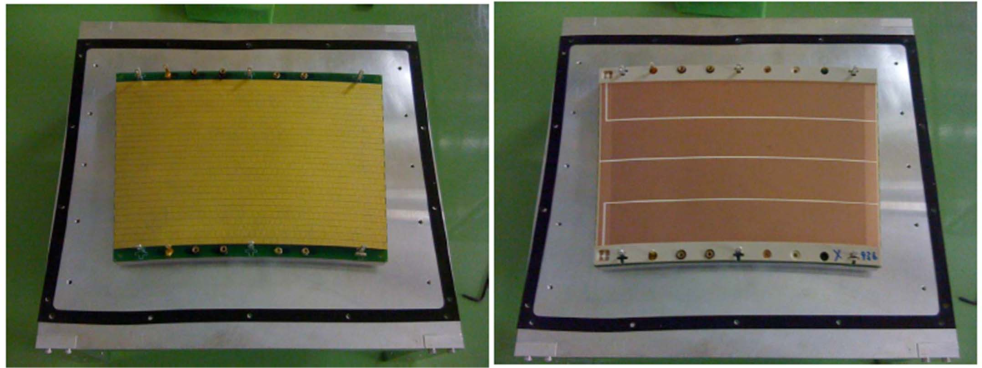
\includegraphics[width=0.9\textwidth]{Tracker/TPC_Bonn/plots/TPC-AG_Fig1asaingempicture}
  \caption{Asian GEM picture: left - anode pad plane; right - segmented cathode.}
  \label{fig_Fig1asiangempicture}
\end{figure}

Particles from the interaction point passing
between the modules may not be detected if they have very high momenta. Therefore, the Asian module foresees no frame along
the sides and extends the sensitive
area up to the edge of the backframe. To ensure a flat mounting of the GEMs, they are stretched on both the upper
and lower arcs (as seen in figure \ref{fig_Fig1asiangempicture}) which are made of a stiffer material:
GEMs with an insulator of \SI{100}{\micro\meter} Liquid Crystal Polymer (LCP)
covered with \SI{5}{\micro\meter} copper on both sides were produced by a company named SciEnergy.
The holes were
produced by \ce{CO2}-laser drilling after which they were carefully cleaned by dry etching to remove potentially
conductive residuals from the insides of the holes. The
hole pattern is identical to standard CERN GEMs. Because of the thicker material also higher gas gains per GEM
can be reached and a double GEM
structure is used and considered to be sufficient.
The two GEMs are mounted with an induction gap of \SI{2}{mm} and a transfer gap of \SI{3}{mm}.

The pad size is $1.2 \times \SI{5.4}{mm}$ and there are 28 pad rows with a total of 5152 pads.
From the beginning the use of an ion gate
(see subsection \ref{chap:TPC_sec:gating}) was envisaged and, thus, the level of the first GEM was designed
to be 1 cm below the nominal module height allowing for a later addition of the gate. To absorb the strength necessary
to stretch the GEMs and the gate, strong metal poles were implemented at the top and bottom arc.

\subsubsection{Recent Milestones}

All modules have been tested in the Large Prototype at DESY. The experience gained during all test beam periods as
well as the best transverse spatial resolution is described next. The testbeam measurements have used
the gas mixture of Ar-\ce{CF4}(3\%)-isobutane(2\%). The electric drift field was set in most cases to
E=\SI{230}{V/cm}, which is close to the maximum of the drift velocity, and alternatively to
E=\SI{130}{V/cm}, which is the minimum of the transverse diffusion.
The Asian modules were also measured using a laser system, in order to analyze the distortions.
The laser beam was scanned across the module, and the deviations were compared with calculations and are understood.

The Asian groups built three modules and made several test beam measurements at DESY (2009, 2010, 2012).
The first campaigns were dominated by very strong field distortions because of the mounting pins and the bare frames.
After introducing the field shaper, the distortions are comparable to the ones of other techniques used for modules.
The transverse spatial resolution is shown in figure \ref{fig_Fig2asiangemresolution}, where the measured spatial
resolution of a single row in the middle of a module can be seen.

\begin{figure}[!htb]
  \centering
  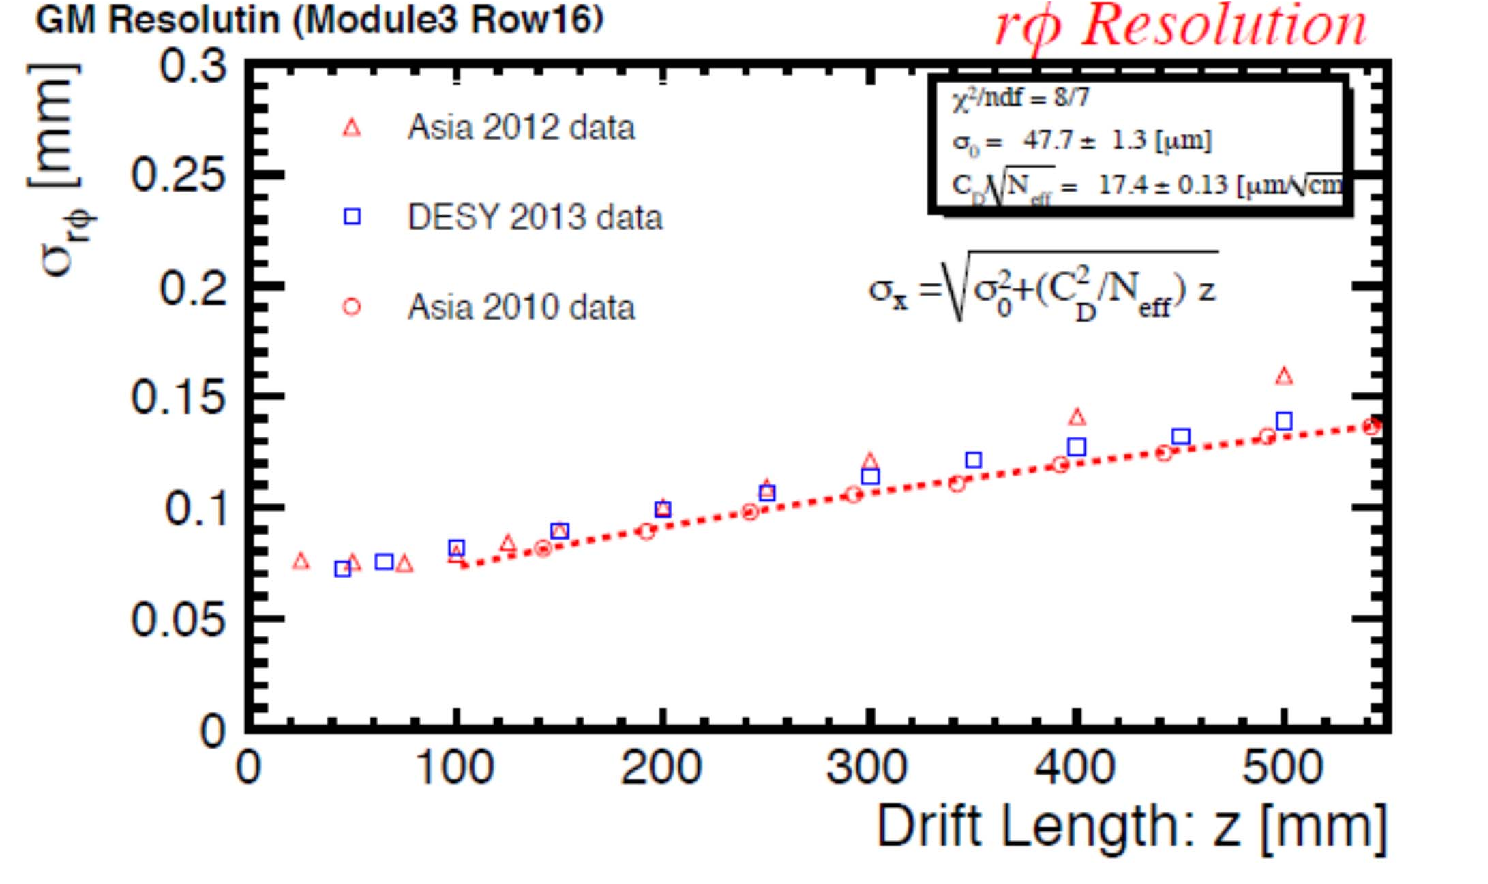
\includegraphics[width=0.9\textwidth]{Tracker/TPC_Bonn/plots/TPC-AG_Fig2asiangemresolution.pdf}
  \caption{Resolution measured for the Asian GEMs, and compared with a result for the DESY GEMs.}
  \label{fig_Fig2asiangemresolution}
\end{figure}

In this context an analytical formula was developed to predict the spatial resolution of a TPC. This formula includes
not only the effect of diffusion, angle,
noise and a finite pad-size, but also the influence of the electronics threshold, number of effective primary electrons,
the Polya-parameter of the gas
amplification, cross talk between pads and signal lines, charge loss because of attachment and the pad response function
are taken into account. All
these parameters can be varied and, if correctly chosen, describe well the measured data.

Finally, one other important observation was the HV micro-discharges on the Asian GEMs, with associated gain drops,
and investigations of this problem are summarized here.

To minimize the energy released in a discharge, the GEMs were segmented into four arcs, each with an area of
about $\SI{100}{cm^2}$ (figure \ref{fig_Fig1asiangempicture}, right).
Studies of the micro-discharges for the various types of GEMs were measured under a controlled environment.
The \SI{100}{\micro\meter} Asian GEMs discharged frequently, while the DESY \SI{50}{\micro\meter} GEMs (made by CERN) had little or no
discharges. For the \SI{50}{\micro\meter} GEMs, there is no significant difference of
the discharge rate between different types of GEMs. It is noteworthy that, at low gain, the \SI{100}{\micro\meter} GEMs
had a discharge rate which is almost the same as for the \SI{50}{\micro\meter} GEMs. The water content in the gas does not seem to
influence the
discharge rate, and long-term measurements are in progress.


\subsubsection{Future Plans}

In the future, it is planned to:\\
$\bullet$ understand better the reasons for the micro discharges and eliminate them, and \\
$\bullet$ construct a full scale Asian module with gate.

\subsection{Module type B, ``DESY Module''}
\label{chap:TPC_sec:DESY_gems}
Most recent update: 2016-03-28 \\
Contact person: Ties Behnke (email: ties.behnke@desy.de)\\

The goal of module type-B is a maximal coverage of the endplate with minimal dead area and a low material budget. It relies on thin ceramic frames to support the GEM foils on top of the readout plane \cite{Hallermann:2010zz,2012arXiv1202.6510D}, see figure \ref{fig:moduleAssembled}. The high stiffness of the ceramic frame allows the construction of very thin frames, which in turn minimize the dead areas of the module. With the current design only $\sim5\%$ of the active area is taken by the support structure and gaps between modules, the rest is sensitive area. The design of the system allows the simple stacking of GEM foils to build up compact, light weight self supporting multi-GEM modules. The development of this module type is led by DESY.

\begin{figure}[htb!]
\begin{subfigure}[b]{0.48\textwidth}
\includegraphics[width=\textwidth]{Tracker/TPC_Bonn/plots/TPC-DG_GemModule_Explosion.pdf}
\caption{}
\label{sfig:moduleExp}
\end{subfigure}
\hfill
\begin{subfigure}[b]{0.48\textwidth}
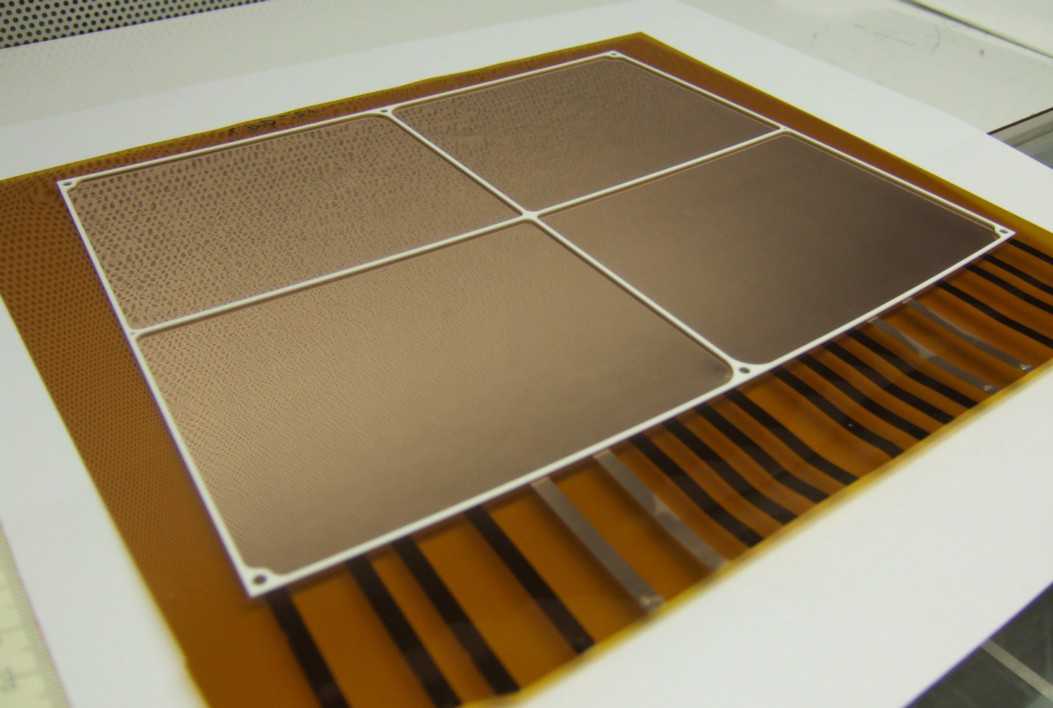
\includegraphics[width=\textwidth]{Tracker/TPC_Bonn/plots/TPC-DG_GemGrid.png}
\caption{}
\label{sfig:moduleGEM}
\end{subfigure}
\caption [Readout Module GEM]{\small \protect\subref{sfig:moduleExp})~Exploded view of one module showing the sequence of GEM foils and ceramic frames. \protect\subref{sfig:moduleGEM})~GEM foil with ceramic frame support used in the construction of the modules.}
\label{fig:moduleAssembled}
\end{figure}

\subsubsection{Recent Milestones}
Over the last years several test-beam campaigns took place and exposed three GEM based modules to test beam. Extensive data sets were collected with and without magnetic field, at different working points, and at different angles between the TPC and the beam.

For the first time the data taken were used in a global attempt to determine and correct field distortions. The Millepede-II \cite{Blobel20065,millepedeWiki} program was used to perform this global fit. First results indicate that distortions as large as several millimeters can be well corrected, see figure \ref{sfig:1Tdistort}. The resolution obtained both in $r\text{-}\varphi$ and $z$ behave as expected, and, if extrapolated to the running conditions at the ILC, meet the requirements, see figure \ref{sfig:resextrapol}.

\begin{figure}[htb!]
\begin{subfigure}[b]{0.48\textwidth}
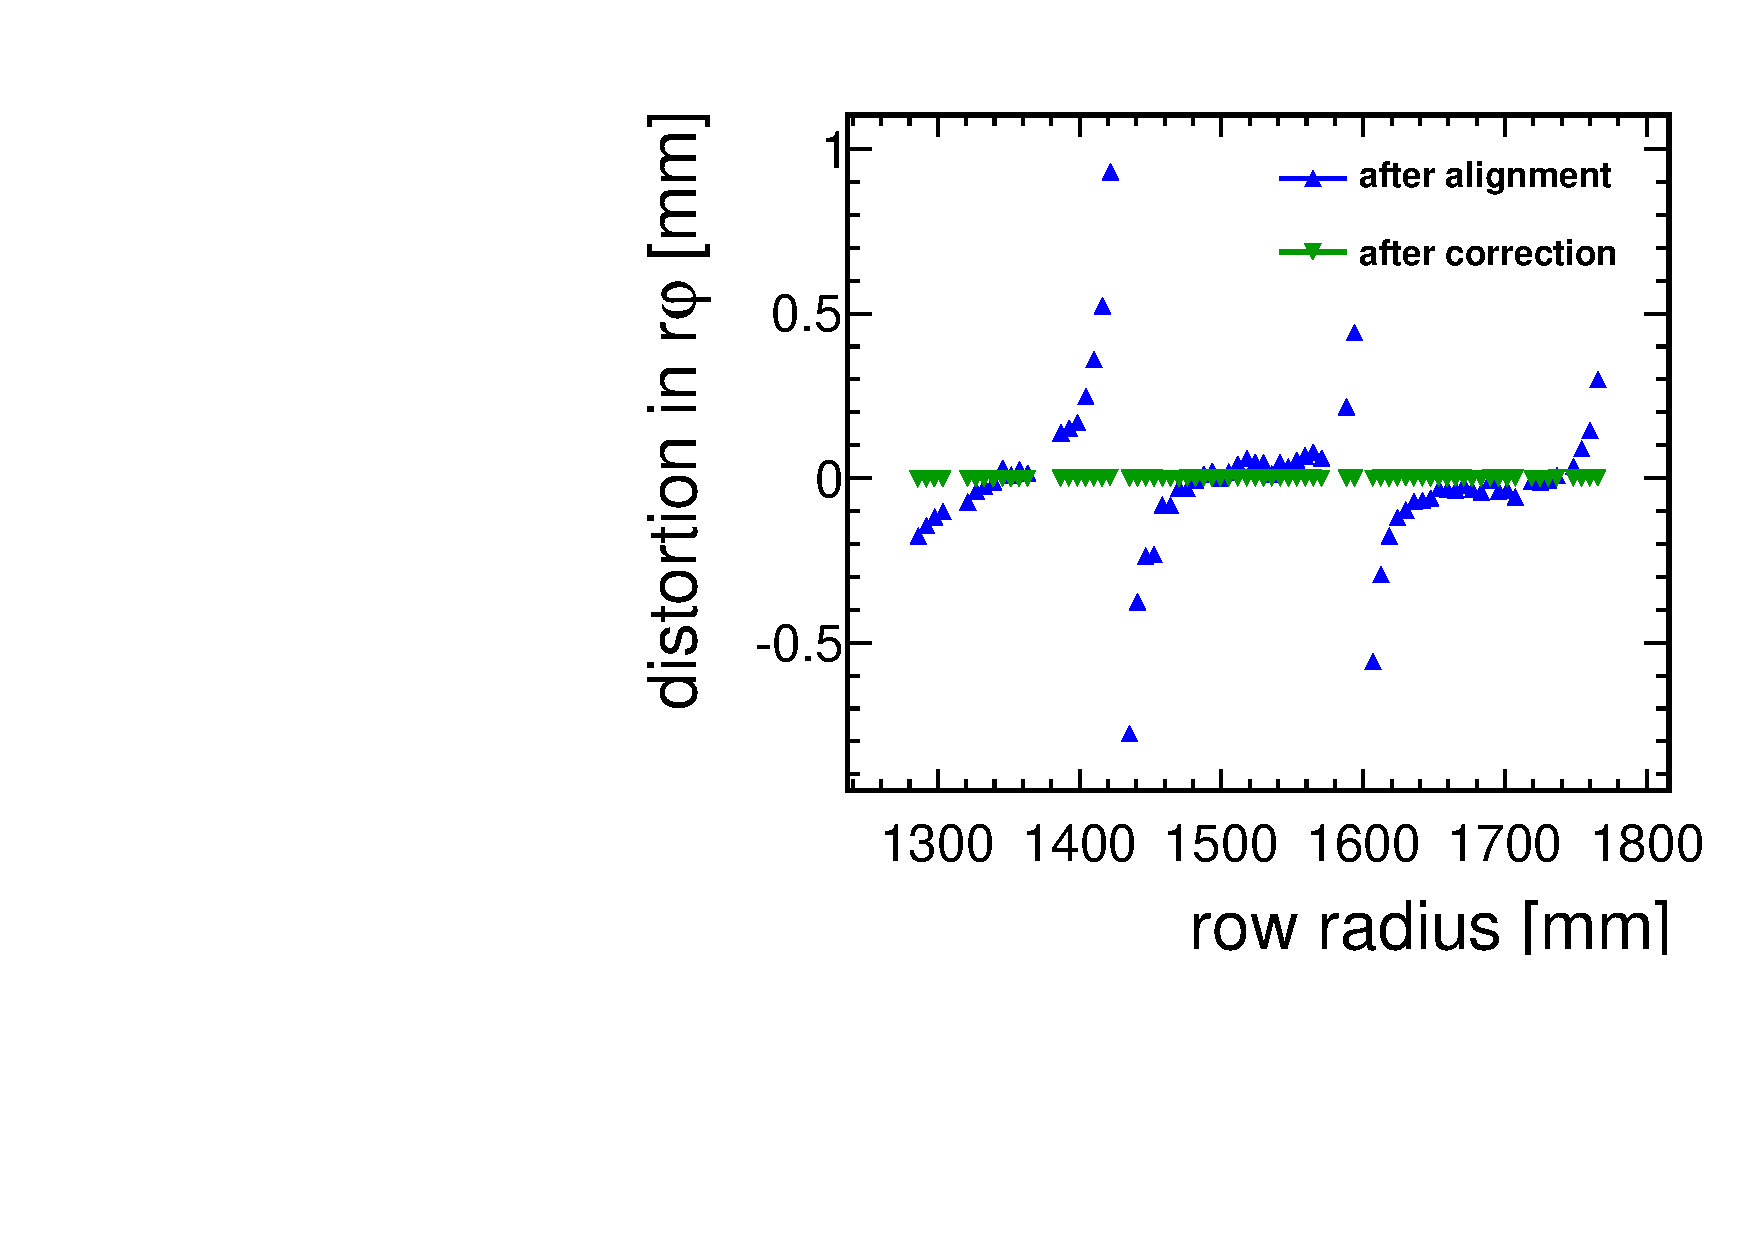
\includegraphics[width=\textwidth]{Tracker/TPC_Bonn/plots/TPC-DG_distortionAlignmentPaper1Tdistcor.pdf}
\caption{}
\label{sfig:1Tdistort}
\end{subfigure}
\begin{subfigure}[b]{0.48\textwidth}
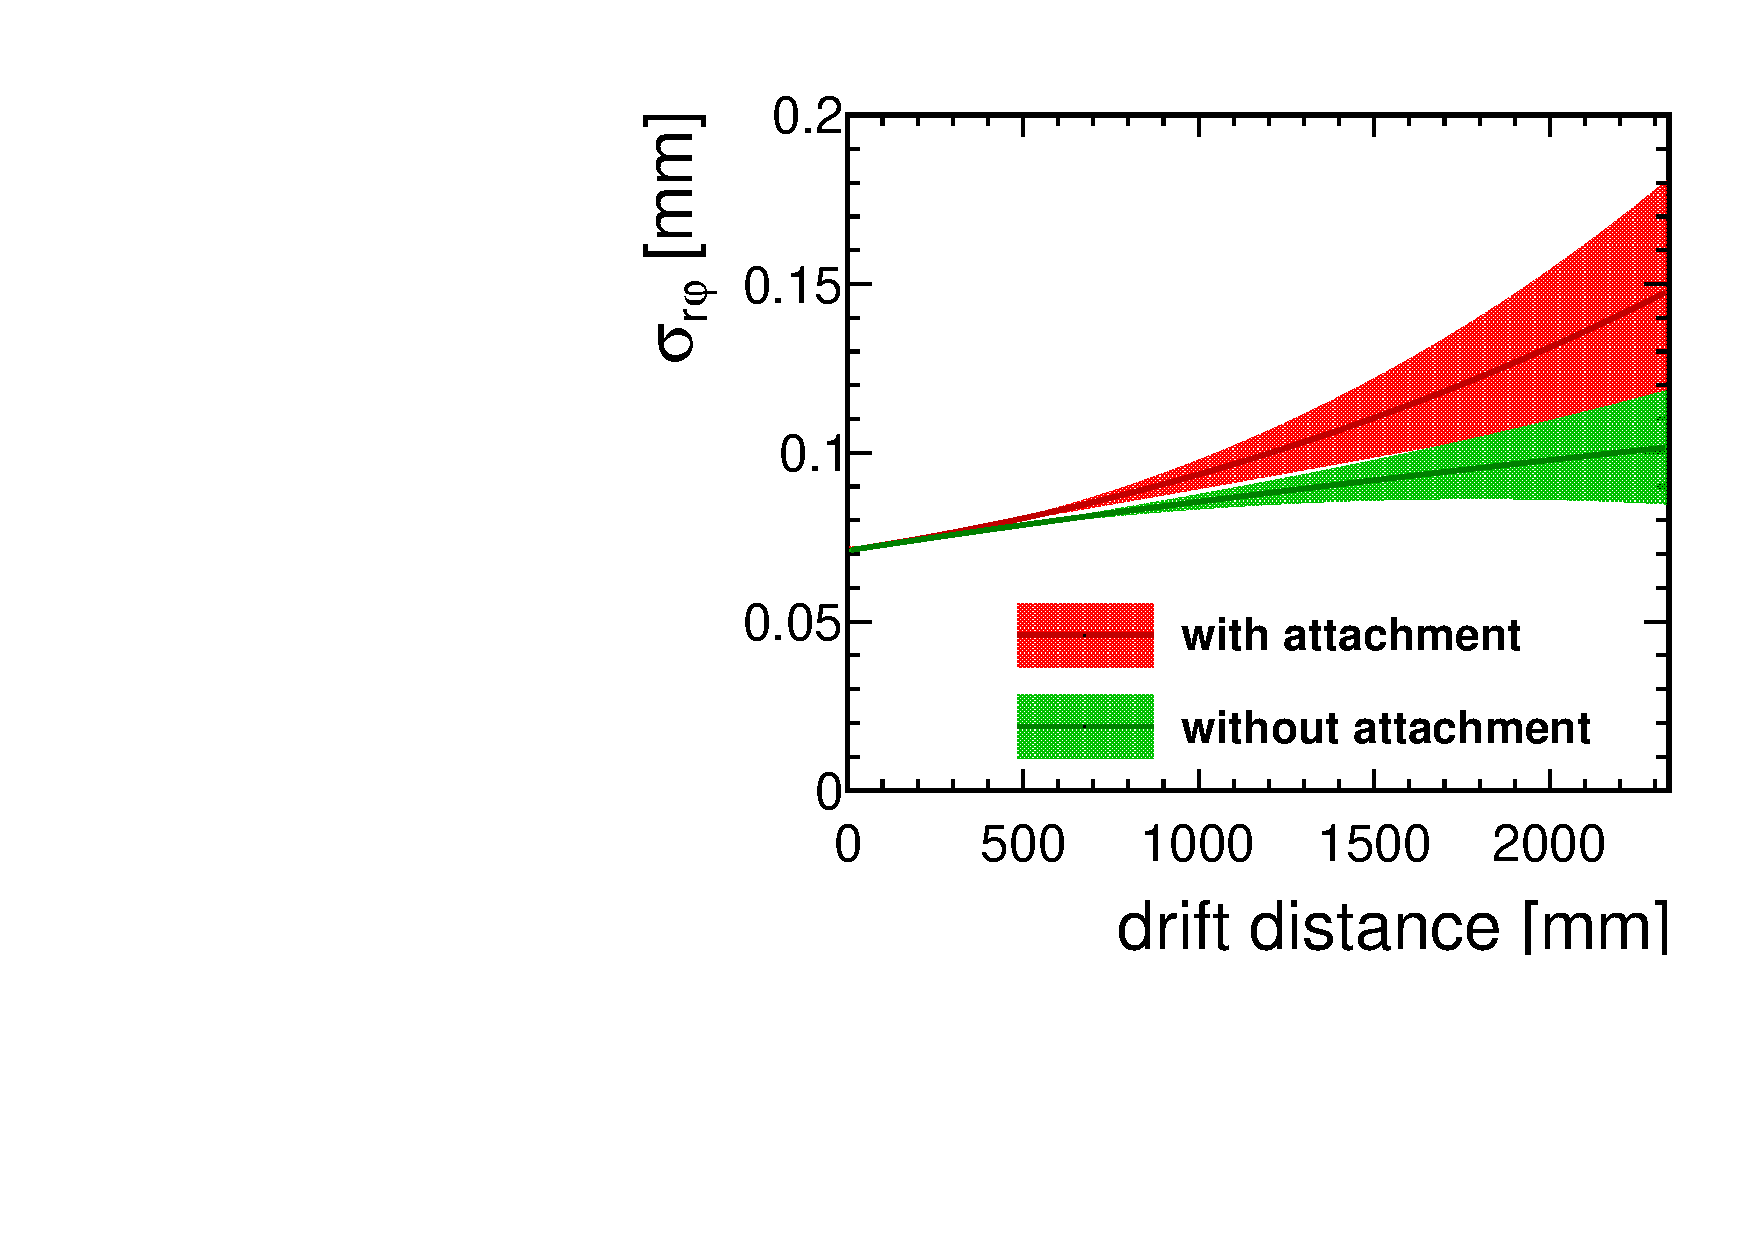
\includegraphics[width=\textwidth]{Tracker/TPC_Bonn/plots/TPC-DG_xyResolutionExtrapolated.pdf}
\caption{}
\label{sfig:resextrapol}
\end{subfigure}
\caption{\small \protect\subref{sfig:1Tdistort})~Alignment and distortion correction: mean hit position in $r\varphi$ with respect to the track position at \SI{1}{T} versus pad row radius. In blue after alignment correction, in green after distortion correction. \protect\subref{sfig:resextrapol})~Point resolution: extrapolation to a magnetic field of \SI{3.5}{T} based on parameters measured with the Large TPC Prototype at \SI{1.0}{T}. Plotted over the full ILD TPC drift length of \SI{2.35}{m} including 1 \sigma error bands. In red with the measured attachment rate, in green without any attachment.}
\label{fig:align1Tdistort}
\end{figure}

The field homogeneity was in addition studied in dedicated laser runs \cite{Zenker:2014qra}. A UV laser illuminates the cathode plane in the TPC, on which dots are placed made from a material with a small work function. The laser light extracts electrons at the position of the dots. These electrons are then drifted towards the anode, and are measured. From the dislocations of the dots relative to the known position on the cathode, the integrated effect of field distortions in the TPC volume can be measured.

Extensive simulations of the behavior of the GEM foils in case of electrical breakdown were performed. They showed that a strong coupling exists between the different regions of the GEM foil. In some cases these couplings can trigger secondary trips in the module, which in rare cases can damage the GEM. A protection circuit is currently under development and will be tested in the near future.

%\subsubsection{Engineering Challenges}
\subsubsection{Future Plans}

By now two generations of these modules have been developed and successfully tested. The main issues which are going to be addressed in the next 1-2 years are
\begin{itemize}
\item re-optimisation of the support structure for maximum mechanical strength and minimal interference with the readout
\item development of a protection scheme which will ensure safe operation of the module even in case of high-voltage trips.
\item optimization of the field-shaping integrated into the module, to minimize field distortions close to the module and at module boundaries.
\item integration of a GEM based gate on top of the current amplification structure, based on the recent developments at KEK.
\end{itemize}
It is planned that within the next six months a third generation module design will be developed and several modules built which will address these challenges.

\subsubsection{Engineering Challenges}
%The GEM based modules face rather similar engineering challenges. Among the most important one is the optimisation of the overall mechanical structure, to provide adequate mechanical strength, without introducing excess dead material.
A detailed study is ongoing to understand and quantify the mechanical behavior of the ceramic frame GEM system. Bending tests have been performed, and compared to simulations. The interference between the mechanical properties and the electrical properties are studied. Measurements of the flatness of the module are being done, and will provide input for the next design iteration.
The fabrication of the ceramic frames which is currently done by laser cutting from solid sheets of ceramic will be studied. Possible alternatives are 3D printing of the frames. Improvements in the laser cutting technology might allow thinner frames, without loosing stiffness.

Another open question is the distribution of the high voltage from the endplate to the different GEM layers. The current solution is rather labour intensive, and relies heavily on the skills of the person doing this connection. Faults are difficult to find, and even more difficult to repair. Here new solutions are being sought, which are more easily to produce, more reliable, and will give better high voltage security. Connected to this are the protection schemes against accidental high voltage discharges, which are still not perfect.

As discussed in section \ref{chap:TPC_sec:gating}, a gating GEM will be implemented as part of the amplification scheme. This gating GEM needs to be mechanically integrated into the module.

Currently a gap of about \SI{2}{mm} exists between neighboring modules. This gap introduces significant field distortions \cite{Zenker:2014qra}. They are partially compensated by a field shaping strip on the outside of each module. However a better and more robust solution would be to further minimize the gap between modules. Doing so will need improvements of the high voltage distribution, as discussed above, but also of the overall mechanical integration of the modules into the endplate.

%\subsection{Applications Outside of Linear Colliders}


\section{Resistive Micromegas}
\label{chap:TPC_sec:micromegas}
Most recent update: 2016-03-28\\
Contact person: Paul Colas (email: paul.colas@cea.fr)\\

\subsection{Introduction}
First Micromegas prototypes were built with a micro-mesh stretched on a frame, and kept on top of
a segmented anode at a fixed distance of \SI{50}{\micro m}. The gap is defined by spacers manufactured
by photo-lithographic techniques. Early tests confirmed that, due to ``hodoscope effect'' a resolution
down to \SI{100}{\micro m} could not be reached \cite{Arogancia:2007pt}. This triggered studies with charge spreading
developed at Carleton University~\cite{Dixit:2003qg}.
The first resistive material was an AlSi CERMET deposited on a Mylar foil and glued at
\SI{90}{\degreeCelsius} with layer of melting polymer~\cite{2007NIMPA.581..254D}. Later on, a more robust resistive material was
used: the Dupont-de-Nemours Carbon-loaded Kapton. Novel way to manufacture the Micromegas detector
were perfected by the Saclay group in partnership with CERN.


\subsection{Recent Milestones}
From 2008 onward, tests with resistive Micromegas were performed in the Large Prototype. From 2008 to 2010
a single module sitting in the middle of the endplate was tested, with dummy modules all around. The 1726 pads, each about \SI{3}{mm} wide
and \SI{7}{mm} long,
were arranged in 24 lines and 72 radial columns, with 2 pads sacrificed to bring the high voltage to the mesh
through the PCB. The standard electronics from the T2K/ND280 neutrino experiment based on the AFTER chip
was used, connected through 20 to \SI{40}{cm} long flat cables~\cite{6418152}.
To minimize the dead area, the so-called ``bulk'' \cite{Giomataris:2004aa} process was used to fix the
mesh on the PCB: in this process a stainless-steal mesh is held by polyimide pillars sandwiching the mesh, melt together
through the mesh. This makes a robust and dust-proof detector, with only \SI{2}
{mm} taken by a grounding ring at the periphery of the module. This ring is used to fix the potential of the resistive anode all around.

Data taken in this 1-module configuration allowed several resistive coatings to be tested. Resistive pastes were discarded, as
their electrical properties were not uniform enough and lead to distortions on the hit position. Carbon-loaded Kapton gave
very good results, with a resolution down to \SI{70}{\micro m} at zero drift distance.

Starting in 2011, a completely new integration of the electronics has been carried out to allow the simultaneous operation
of 7 modules. Naked chips were directly wire-bonded on cards. All the protection of the electronics was removed, this functionality
being fulfilled by the resistive coating. The ADC was moved from the front-end to a mezzanine card, all the electronics fitted just behind the module.
At the same time the noise and the power consumption were lowered by 25\%. To connect a module with 1726 channels, only
3 cables need to be connected: a High Voltage cable for the gaseous amplification, a low voltage cable to supply the electronics,
and an optical fiber to transport the data and the command parameters to the mezzanine card.
The production of 9 modules (including 2 spares) and their electronics followed a quasi-industrial scheme.

Data with 7 modules were taken in 2014 and 2015, allowing new topics to be addressed, as module alignment and distortions.
ExB effect induces distortions for tracks reconstructed near the module boundary causing
shifts of almost 1 mm for pad hits located at the extremity of the module.


This is
in agreement with the simulations carried out in the Kolkata group and which can be corrected down to \SI{20}{\micro m}.

In 2014 and 2015, a two-phase \ce{CO2} cooling was provided to the 7 Micromegas modules. The two-phase coolant, under a pressure of \SI{50}{bar}, circulates at a temperature close to the ambient.
It consists presently of a serpentine running on the back of the modules, in good thermal contact with Aluminum heat sinks, themselves in contact with the chips. The pipe diameter is less than a millimeter, giving a moderate contribution to the material budget. The unit
which provides the pressurized \ce{CO2} was funded by KEK and designed by a Nikhef-CERN collaboration.
An efficient cooling was observed for more than 80 hours continuously.

In 2015, two new modules were inserted on the endplate. The resistive material of the new
modules was Diamond-Like Carbon obtained by sputtering on a Kapton foil.
This gives a very robust resistive anode, and the procurement of this material, made in Japan, is more reliable
than the Dupont Carbon-loaded Kapton. These two modules showed identical performance as the other modules.

\subsection{Engineering Challenges}
Special care will have to be given to the design of the edge of the modules, to have a uniform potential on the exposed surface of the pad while the boarders of the modules must be grounded.

The adaptation of a gating device at a few cm from the end-plate, or integrated to each module, is a
difficult engineering challenge if a minimal degradation of the performances is to be obtained.


\subsection{Future Plans}
The time structure of the beams will produce positive ion backflow disks moving slowly (at a few \SI{1}{m/s}) towards the cathode. To experimentally address the question of the effect of these ion disks on the drifting electrons, it is projected to produce such
ions by casting UV light to the cathode for a ms every \SI{100}{ms} or so, while observing distortions on cosmic-ray or beam tracks.
Last but not least, the momentum resolution should be evaluated with long tracks from a particle beam, which requires a silicon
tracker inside the magnet to measure precisely the track position and momentum. For the cooling, further integration work is needed, using micro-channels in the detector board and new material choices for the sink.

In summary, the Micromegas TPC R\&D successfully underwent its proof-of-principle phase and the main integration questions are now addressed. They now request targeted design to progress, thus specific project funding.

\section{Pixelized Readout}
\label{chap:TPC_sec:pixels}
Most recent update: 2018-11-01 \\
Contact person: Klaus Desch (email: desch@physik.uni-bonn.de)\\

\subsection{Introduction}
To make the most of the fine pitches of the Micropattern Gaseous Detectors the
readout structure should be adapted to the same feature size. Therefore,
readout ASICs of silicon pixel detectors such as the Timepix ASIC
\cite{Llopart2007485, Llopart2008106} can be placed directly below the gas amplification
stage. In this setup, the bump bond pads normally used to connect the readout
chip to the Si-sensor are used as charge collection pads. In some studies a
triple GEM was used as a gas amplification stage \cite{Bamberger:2006xp, 6359808},
while in others a Micromegas has been built
directly on the ASIC \cite{4526754}. The latter detector type is 
 called GridPix and is produced by using a post-processing technique, which
 guarantees a high quality grid perfectly aligned with the readout pixels. This
 alignment ensures that the complete charge avalanche initiated by a primary
 electron is collected on one pixel. Because of the high signal-to-noise
 ratio both tracking and dE/dx measurement benefit from distinguishing and
 detecting single primary electrons with a high efficiency. This type of
 detector was pioneered by Nikhef/University of Twente (NL). The University
 of Bonn has modified the 
 production process together with the Fraunhofer Institut IZM so that a
 wafer-based production of GridPix detectors is standard by now
 \cite{Koppert2013245}. First tests were done with both
 gas amplification stages by using single ASICs with an active area of about \SI{2}{\centi\meter\squared}. The detectors were operated in laboratories at Nikhef, Saclay, Bonn,
 Freiburg and Siegen to test the working principle. It could be demonstrated
 that the transverse spatial resolution of the reconstructed primary electrons
 was close to the expected diffusion limit of single electrons. 

 \subsection{Recent Milestones}
At the University of Siegen new types of GEMs are being tested in combination
with the Timepix ASIC: GEMs with a carbon coating on the copper electrodes and
GEMs with a ceramic insulator. Both types are tested in a prototype setup and
compared to standard CERN GEMs.

At Nikhef, Saclay and Bonn several projects were carried out to demonstrate
multi-module operation and large area coverage of modules with GridPix
detectors. The new GridPixes were also assembled in 8
GridPix modules for the Large Prototype detector at DESY. Successful test beam
campaigns were performed in 2010 with a single module and in 2013 and 2014 
with two modules \cite{1748-0221-9-01-C01033}. Up to three LP modules
with a total of 160 GridPixes were operated in a test beam. The central module was equipped with 96
GridPixes and the two outer modules had 32 GridPixes arranged to maximize the
lever arm. 
\begin{figure}[!t]
  \centering
  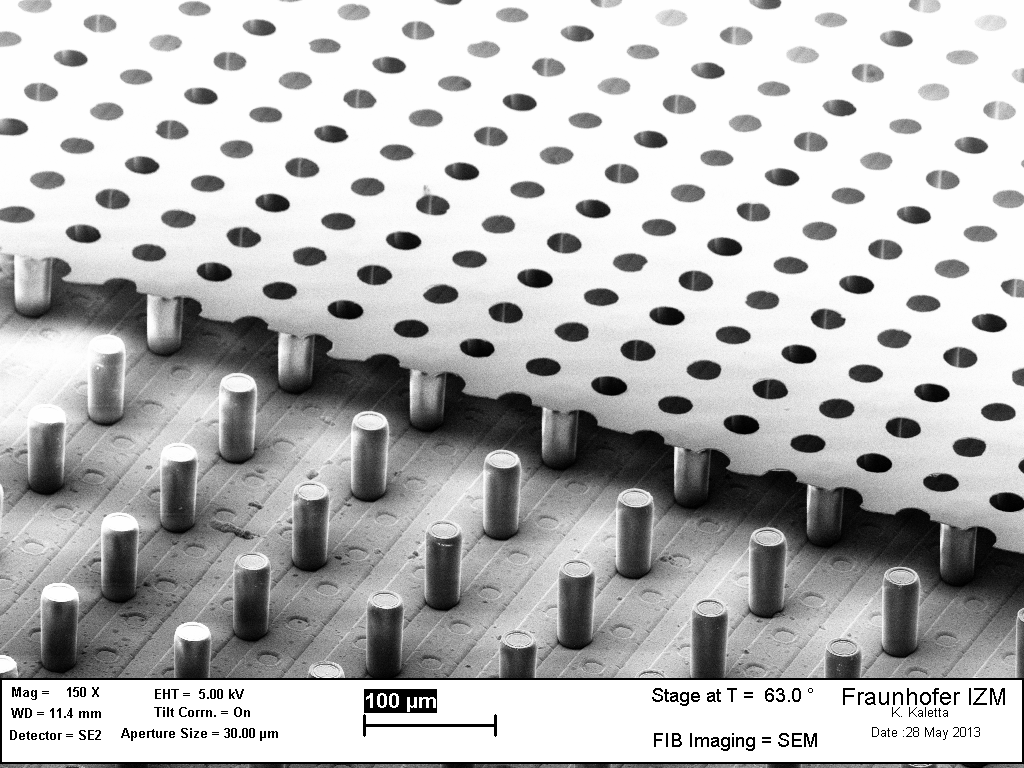
\includegraphics[width=0.45\textwidth]{Tracker/TPC_Bonn/plots/TPC_pixels_GridPix.png}
  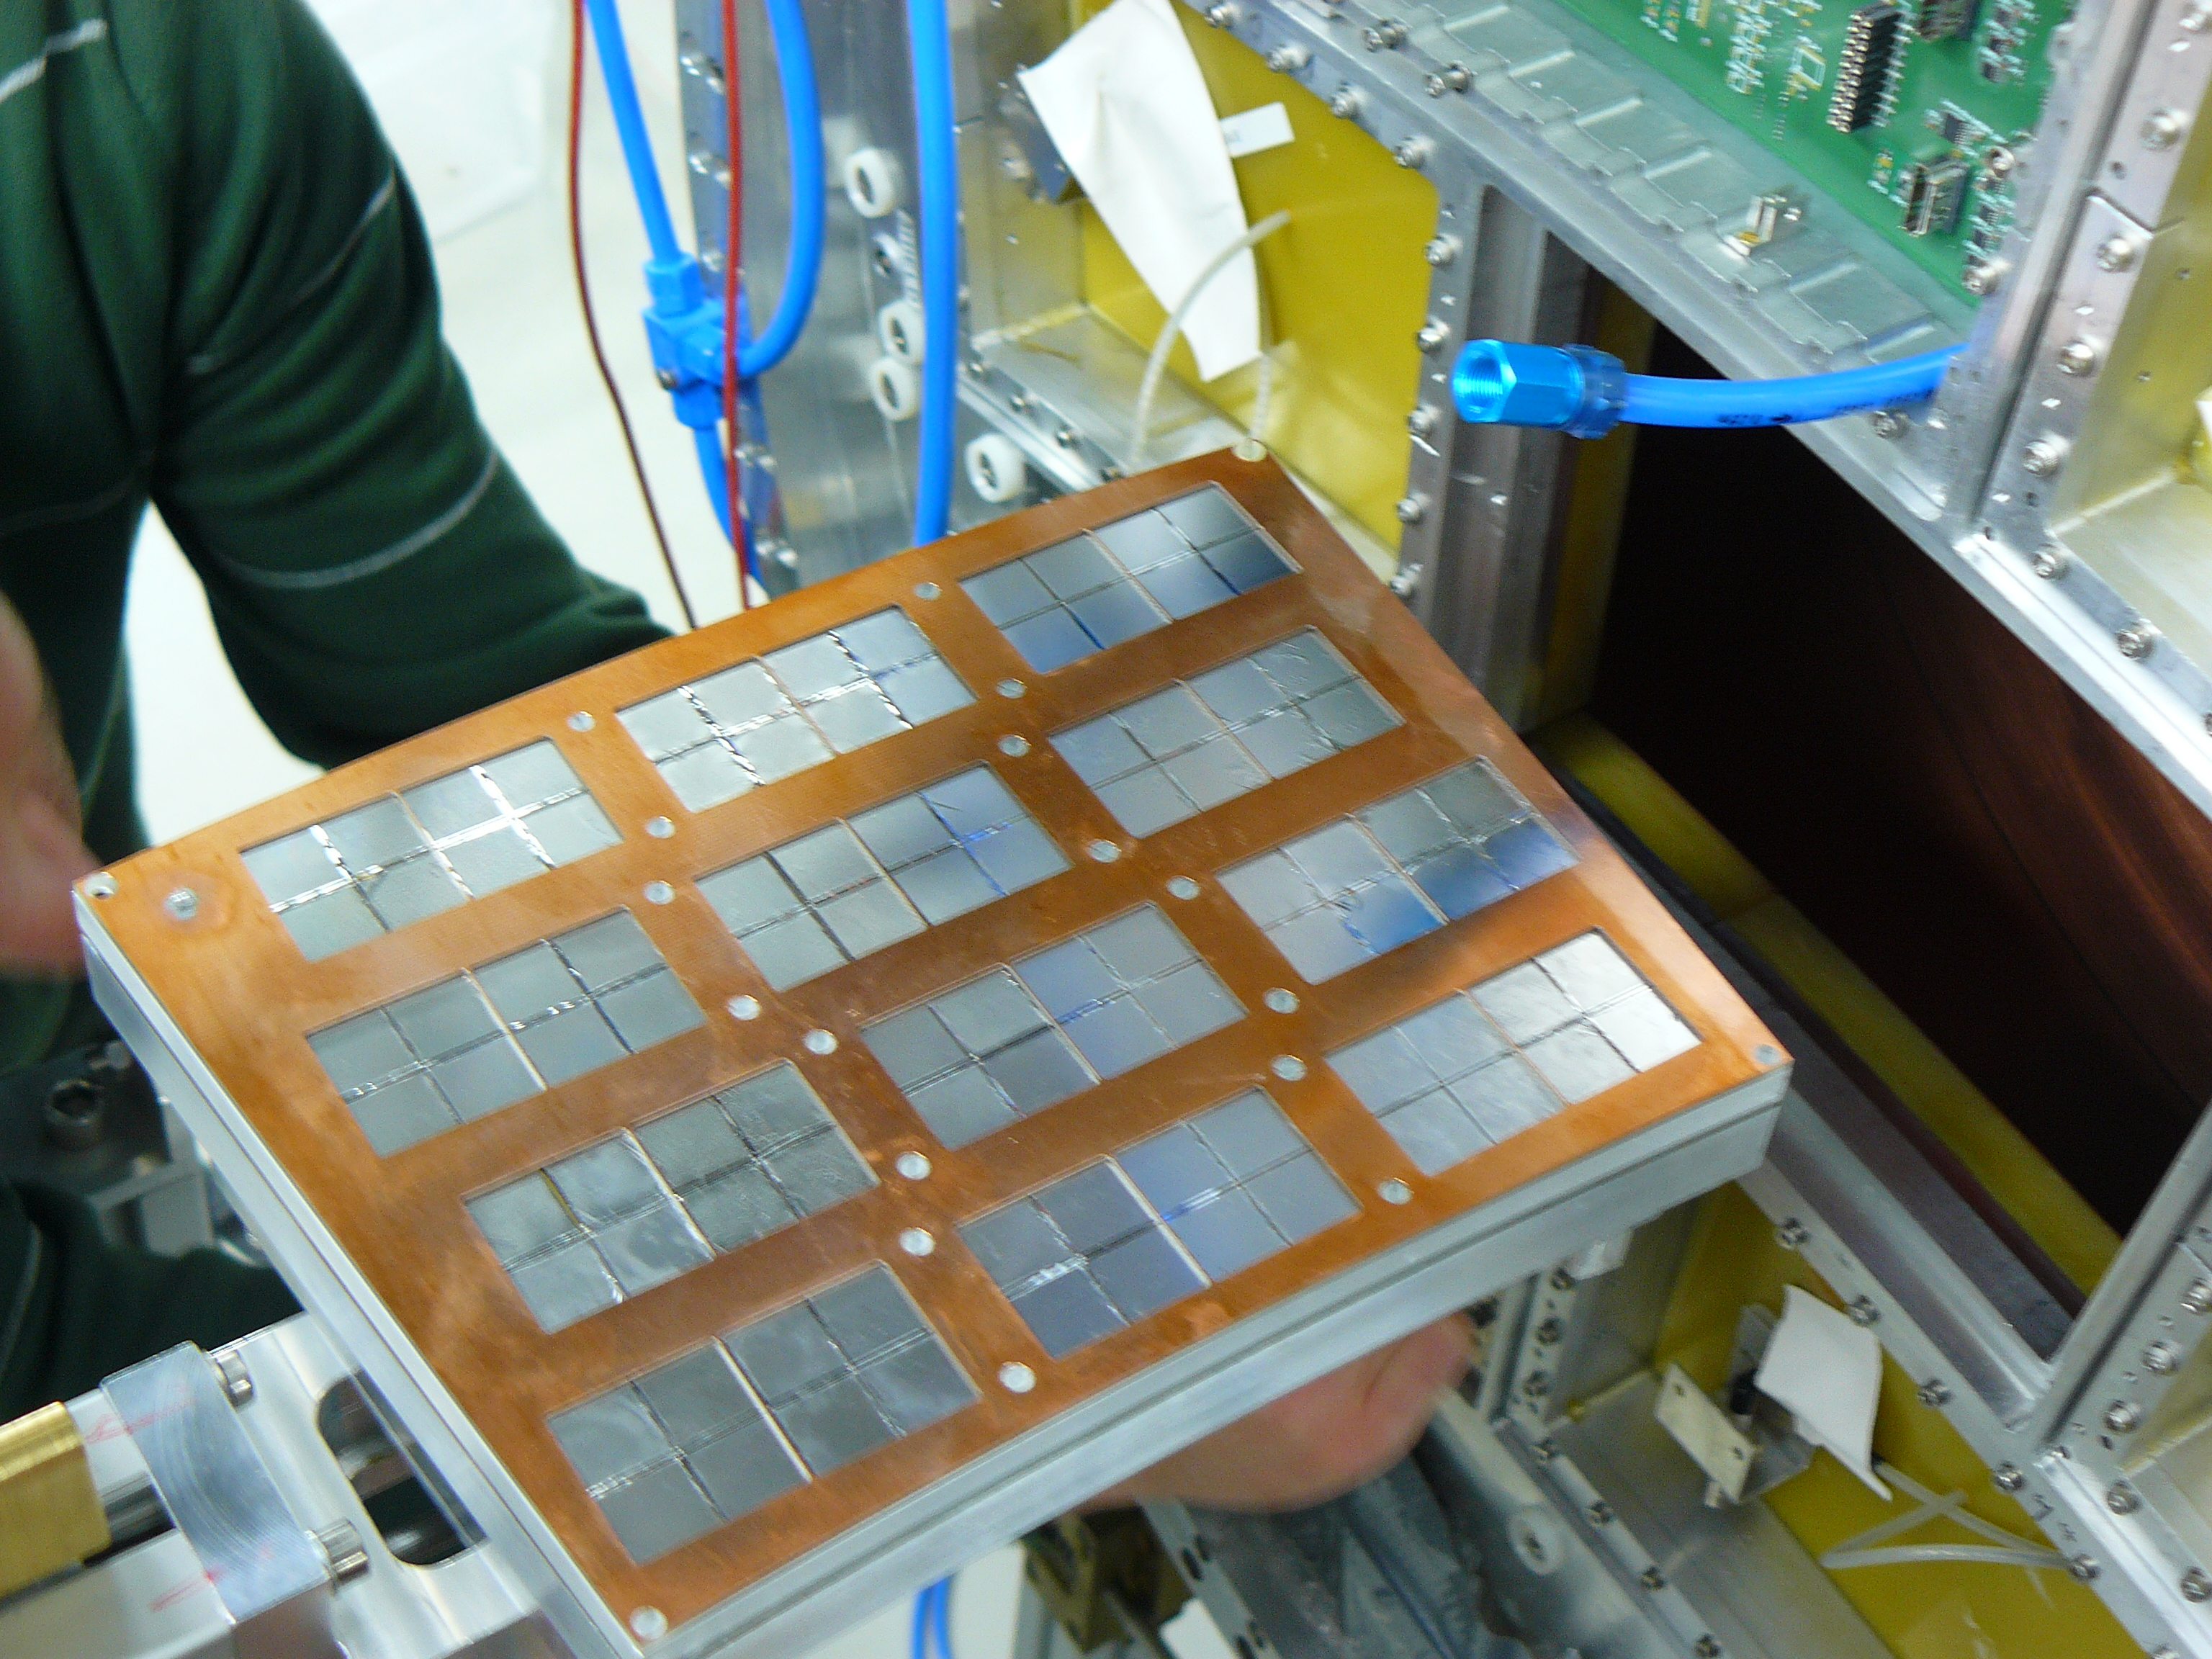
\includegraphics[width=0.45\textwidth]{Tracker/TPC_Bonn/plots/TPC_pixel_complete_module.png}
  \caption{Left: SEM picture of an InGrid detector with a partially removed
    grid, right: Fully equipped LP module with 96 GridPix detectors is being
    mounted in the LP.}
  \label{fig_TPC_pixels_1}
\end{figure}

This setup served as a demonstrator that larger areas ($\sim$\SI{400}{\centi\meter\squared}) could be produced and operated. It was tested in the Large Prototype in March/April of 2015 and operated for more than one week permanently in the
test beam. A total of about 200 runs with more than 1.5 million events were recorded \cite{7889045}.

\begin{figure}[!t]
  \centering
  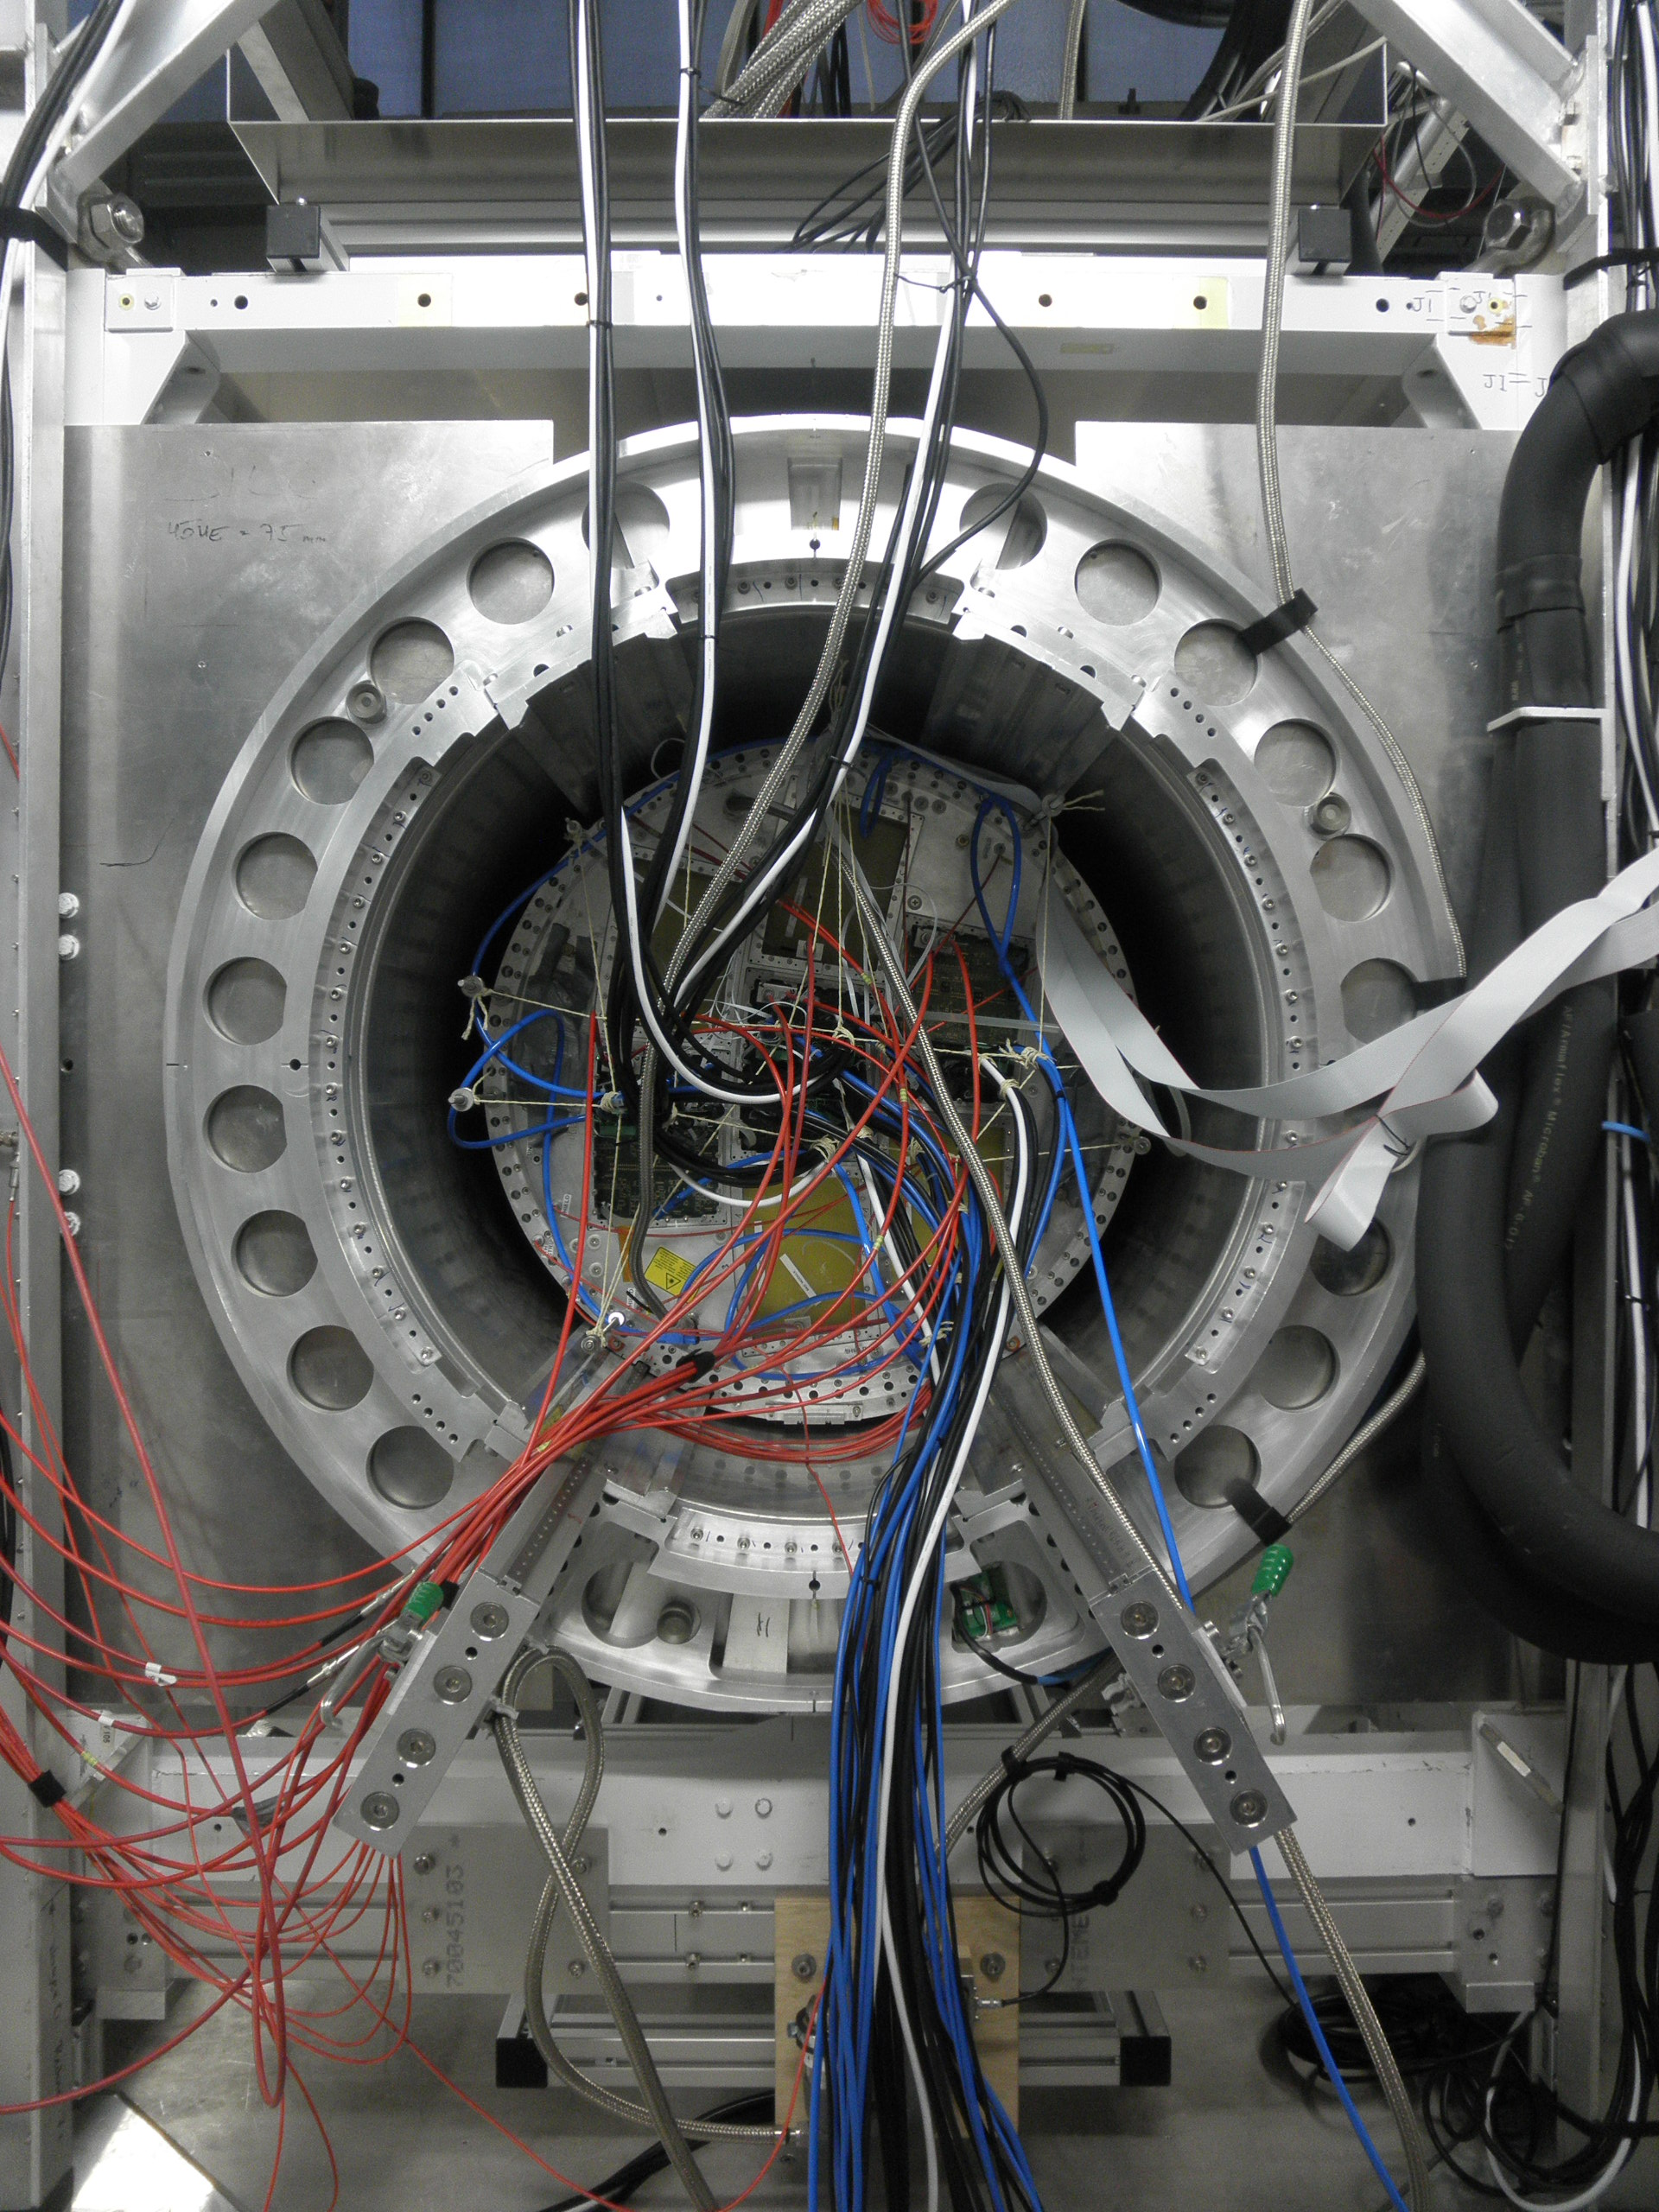
\includegraphics[width=0.28\textwidth]{Tracker/TPC_Bonn/plots/TPC_pixels_LP_GridPixes.png}
  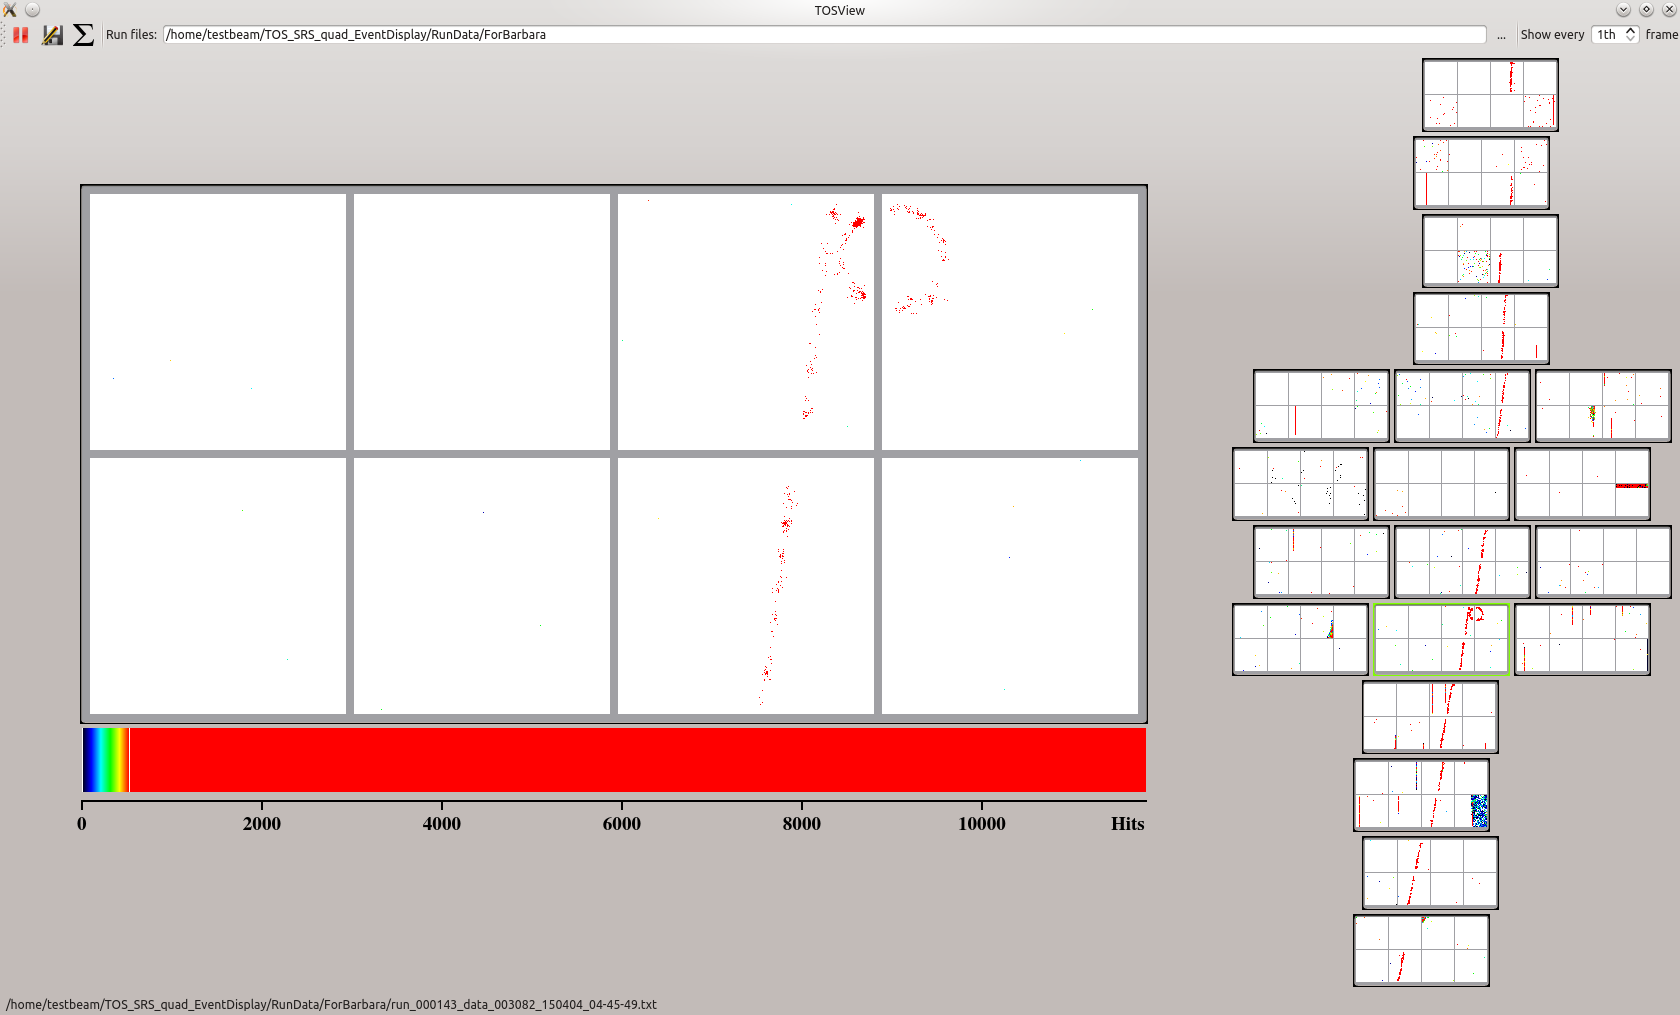
\includegraphics[width=0.62\textwidth]{Tracker/TPC_Bonn/plots/TPC_pixels_event.png}
  \caption{Left: Three modules with 160 GridPix detector mounted on the Large
    Prototype, right: Online event display of a 2 track event recorded with
    160 GridPixes.}
  \label{fig_TPC_pixels_2}
\end{figure}

Nikhef and Bonn have also taken part in designing a successor ASIC of
the currently used Timepix. The new Timepix-3 features several improvements,
which promise a much better performance. In particular it is multi-hit capable,
can record both time and charge of each signal, has a much faster
digitization frequency (\SI{640}{\mega\hertz}) and can be read out  quasi continuously.
Also, the grid design was revised increasing the active area to 97.7\% of the pixel area. First Timepix-3-based GridPix detectors have been built and tested. A testbeam campaign was conducted in July 2017 at the ELSA accelerator in Bonn and a single GridPix detector was exposed to an \SI{2.5}{GeV} electron beam \cite{Ligtenberg:2018sjs}. The performance clearly surpassed the one of Timepix-based GridPixes. In particular the longitudinal spatial resolution could be improved by over one order of magnitude. 
As a next step, in 2018 a quad consisting of four GridPix detector was constructed and
tested~\cite{Ligtenberg:2020ofy}. Special attention was given to the mechanical and electrical design of the
guard structure to maximize coverage and minimize distortions. The distortions in the
precision plane stay below the 13 microns and meet the design specifications of a TPC at a
linear collider. A module consisting of 8 Quads has been constructed and will be tested in
2020.

\subsection{Engineering Challenges}
The production of modules with large area coverage requires to solve four
major technical challenges: 
\begin{enumerate}
  \item The production of a large number of GridPixes with sufficiently good
quality. This has been addressed by the new production method, which is based
on complete wafers. The process was developed in collaboration with the
Fraunhofer Institute IZM at Berlin and yields up to 428 GridPixes per batch (4 wafers). 
\item In particular commercial readout systems are not easily scalable to a large number of chips. This is why Bonn has developed a cheap and easily expandable system based on the Scalable Readout System (SRS) of the RD51 collaboration.
Nikhef developed (partially funded by the AIDA FP7 project) the SPIDR fast readout system for Timepix-3 ASICs \cite{1748-0221-10-12-C12028}.
\item Current water cooling has to be replaced by 2-phase \ce{CO2} cooling.
\item In order to overcome systematic limitations of track reconstruction, field
  distortions caused by tilted chips and only partially covered ground
  potentials need to be mitigated.
\item In order to reduce the ion back flow a gating grid (as discussed below in section~\ref{chap:TPC_sec:gating}) can
be installed. For a GridPix a solution based on a double grid - with a same hole pattern - is possible.
This will reduce the ion backflow continuously(, as e.g. needed for high luminosity Z running
at circular a machine). Both the gating grid and the double grid solution need further
studies and tests.

\end{enumerate}

\subsection{Future Plans}
Currently the main focus is on the analysis of the test beam data. The
challenge of finding and fitting tracks with several thousand hits is quite
different from the standard pad-based TPC analysis. For this a group of people
from Nikhef, DESY, Siegen and Bonn are testing new ideas. On a longer term all
participating institutes are working on software to simulate, reconstruct and
analyze data of the ILD-TPC (i.e. about 10,000 hits per track) so that the
difference in performance between a pad and a pixel-based TPC can be studied. 
On the hardware side a new compact device containing four Timepix-3-based
GridPixes is being developed at Nikhef. This device called Quad minimizes the
dead area and new mounting procedures improve the alignment of the individual GridPixes,
so that a much reduced field inhomogeneity is expected. The construction of a
few fully equipped, engineering modules made of the aforementioned Timepix-3
GridPix Quads is planned.

\subsection{Applications Outside of Linear Colliders}
A seven GridPix detector is taking data for more than 1 year in the CAST
experiment for axion search and is also considered for the successor experiment IAXO.
In collaboration with KVI-CART in Groningen (NL) a system for proton radiography
is being developed using small (gaseous) TPCs based on GridPix detectors, for
accurate 3D proton tracking.

Also a new kind of neutron detector based on the TPC principle is being developed at Bonn. Here, a 8 GridPix readout at one of the endcaps is needed to reach the best possible spatial resolution.

Further applications in e.g. X-polarimetry and direction dark matter detection are envisaged.

% \section{Time Projection Chamber -- GridPix, Bonn}
\subsection{Introduction}
The project studies the pixelized readout of a TPC for the ILD detector. The readout is based on the Timepix ASIC with a triple GEM or Micromegas based gas amplification.

\subsection{Recent Milestones}
The first studies were based on the triple GEM setup with a single Timepix chip. This readout was mounted in a small test detector in the Bonn laboratory. Here, the working principle was tested with a long drift distance. It could be demonstrated that the transverse spatial resolution of the reconstructed primary electrons was close to the expected diffusion limit of single electrons. The results are summarized in the following publications:
\begin{itemize}
\item \fullcite{6359808}
\item \fullcite{4774978}
\item \fullcite{1748-0221-4-11-P11015}
\item \fullcite{Kaminski:2010zzc}
\item \fullcite{Schade2011128}
\end{itemize}

The new focus are GridPix based detectors, where the gas amplification stage is a Micromegas produced in a postprocessing technique, which guarantees a high quality grid well aligned with the readout pixels. This approach was pioneered by NIKHEF and the University of Bonn has modified the production process together with the Fraunhofer Institut IZM so that a wafer-based production of GridPix detectors is standard by now. The new GridPixes were tested on small prototype detectors and also assembled in an 8 GridPix module for the Large Prototype detector at DESY. A successful test beam campaign was performed last year.
\begin{itemize}
\item \fullcite{1748-0221-9-01-C01033}
\item \fullcite{Koppert2013245}
\end{itemize}
The current work is focused on a new LP module with about 160 GridPixes. The central module is equipped with 96 GridPixes and the two outer modules have 32 GridPixes arranged to maximize the lever arm. This setup serves a demonstrator that larger areas (~$\SI{400}{cm^2}$) can be produced and operated. It was tested in the Large Prototype of the LCTPC collaboration in March/April of 2015 and operated for more than one week permanently in the test beam. A total of about 200 runs with more than 1.5 million events were recorded.
For this a number of challenges had to be overcome. In particular commercial readout systems are not easily scalable. This is why Bonn has developed a cheap and easily expandable system based on the Scalable Readout System (SRS) of the RD51 collaboration.

In addition Bonn is developing the software for reconstructing and analyzing the test beam and simulation data. For this the LCTPC software framework of MarlinTPC is used.
\begin{itemize}
\item \fullcite{4774731}
\end{itemize}

Finally, Bonn also takes part in designing new pixel chips. To test the new digitization and readout techniques two test chips were designed in collaboration with N'IKHEF. Then Bonn also contributed to the design of the Timepix successor chip, Timepix3, which is being tested now:
\begin{itemize}
\item \fullcite{1748-0221-5-12-C12005}
\item \fullcite{6748097}
\item \fullcite{1748-0221-9-01-C01052}
\end{itemize}

\begin{figure}
	\begin{minipage}{.49\textwidth}
		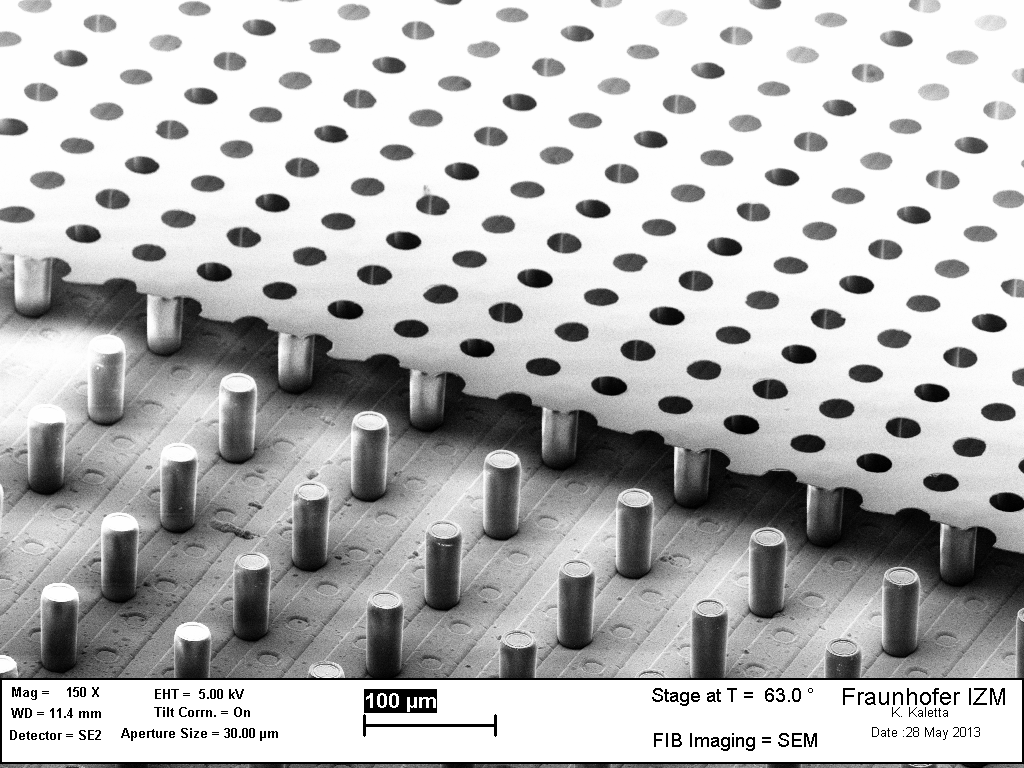
\includegraphics[width=\textwidth]{Tracker/TPC/GridPixes}
		\caption{GridPix detector with a partially removed grid}
		\label{fig:TPC:GridPix:GridPix}
	\end{minipage}
	\hfill
	\begin{minipage}{.49\textwidth}
		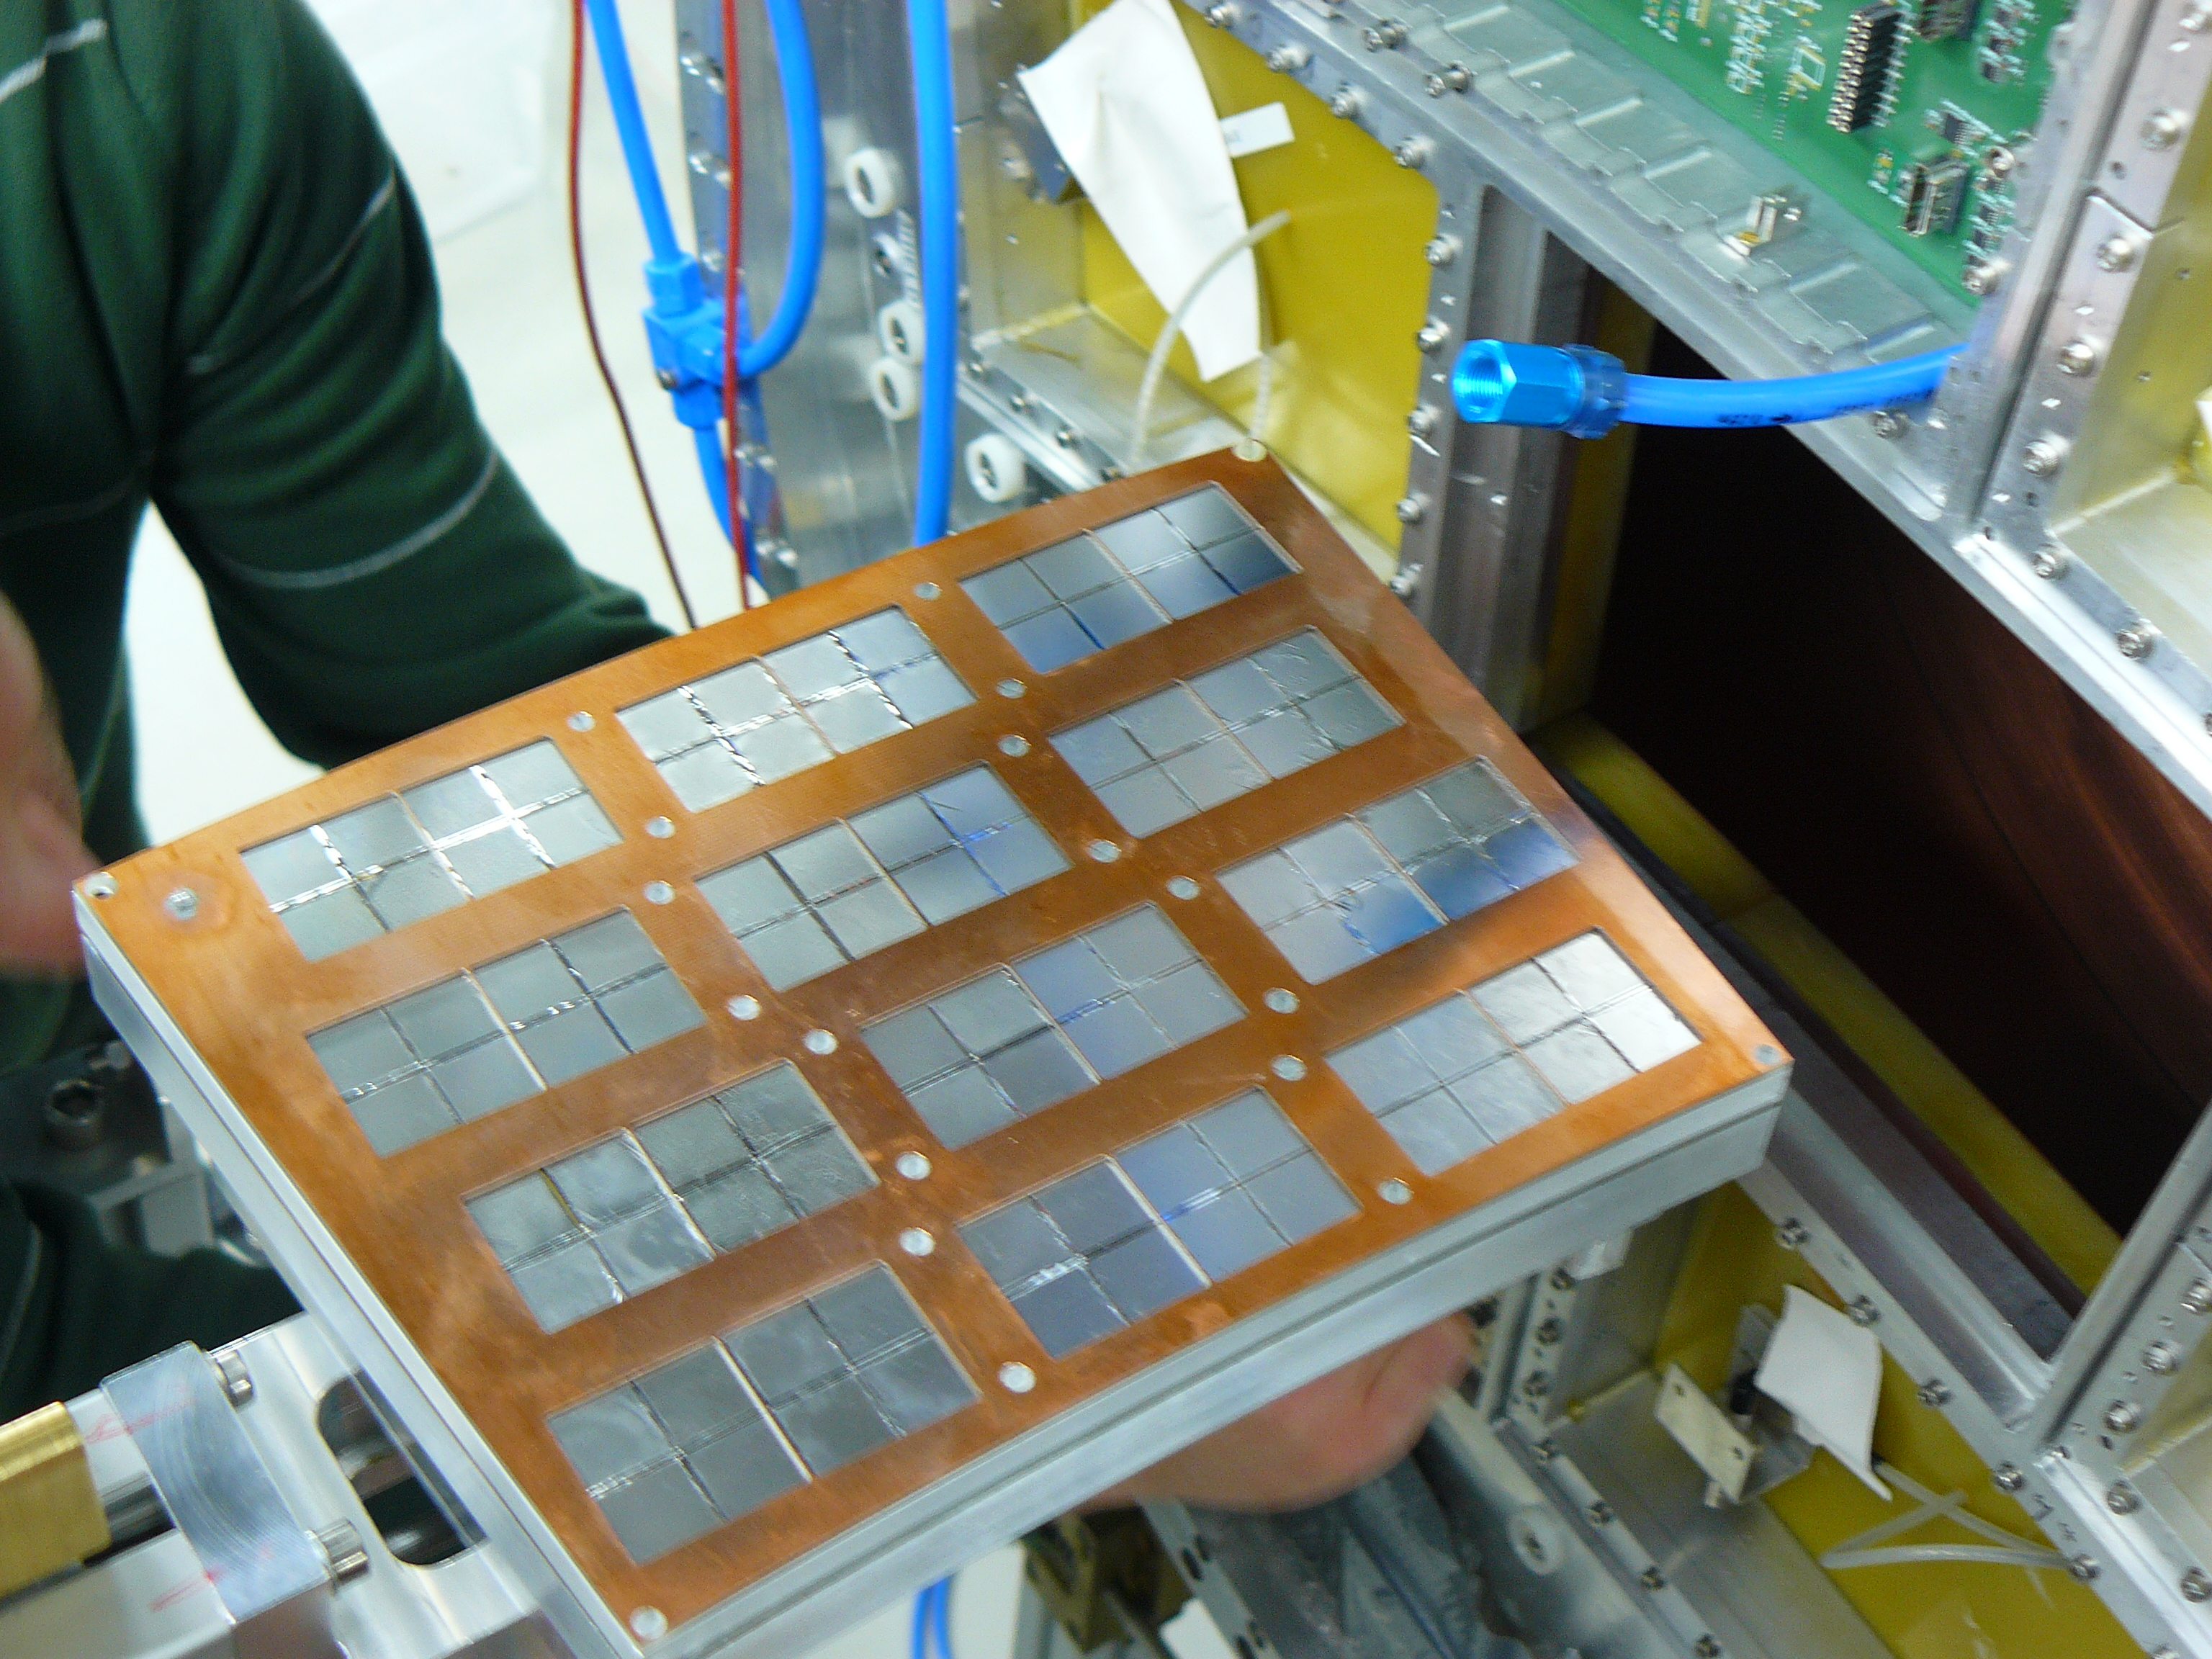
\includegraphics[width=\textwidth]{Tracker/TPC/FullModule}
		\caption{Fully equipped module as it is being mounted}
		\label{fig:TPC:GridPix:module}
	\end{minipage}
\end{figure}

\subsection{Engineering Challenges}
The production of a module with 160 GridPixes requires 4 main components:
\begin{enumerate}
	\item The production of a large number of GridPixes with sufficiently good quality. This has been addressed by the new production method, which is based on complete wafers. The process was developed in collaboration wit the Fraunhofer institute IZM a Berlin and yields up to 400 GridPixes per batch. Figure~\ref{fig:TPC:GridPix:GridPix} shows a GridPix detector with a partially removed grid.
	\item The challenge of the readout is being addressed by the new readout system as described above.
	\item The distribution of the LV power to all ASICs which can reach peek values of \SI{85}{A} at \SI{2.2}{V} was studied in a Master thesis.
	\item Cooling of the ASICs was done by cold water.
\end{enumerate}


\subsection{Future Plans}
Currently, the main focus is on the analysis of the test beam data. The challenge of finding and fitting tracks with several thousand hits is quite different from the standard pad-based TPC analysis. On a longer term all participating institutes are working on software to simulate, reconstruct and analyze data of the ILD-TPC (i.e. about 10,000 hits per track) so that the difference in performance between a pad and a pixel-based TPC can be studied.
On the hardware side we are interested in replacing the Timepix ASIC by the Timepix3 ASIC and produce GridPix detectors with this improved chip, which promises a much better performance, since it is multi-hit capable, can record both time and charge of a each signal and has a much faster digitization frequency. There are also some ideas of how to improve the grid structure and make it more reliable.

\section{Ion Backflow and Gating}
\label{chap:TPC_sec:gating}
Most recent update: 2016-03-28 \\
Contact person: Akira Sugiyama (email: sugiyama@cc.saga-u.ac.jp)\\

\subsection{Introduction}

The distortion of particle tracks due to the accumulation of positive ions in the drift space is the well-known
issue for TPCs, whereby the ions are generated in the gas amplification region and drift back into the TPC drift volume.
Although this ion back flow is much suppressed for the MPGD technology, compared to the earlier MWPC TPCs, it can
still cause significant distortion of tracks when the particle density is high.

Because of the bunch-train structure of the ILC beams (i.e., a  train of ca. 1300 to 2600 bunches during
about \SI{1}{ms}
and a train-repetition rate of \SI{5}{Hz}), the ions flow back from the gas amplification and will form a few discs
of about \SI{1}{cm} thickness in the TPC drift volume where they slowly drift toward the TPC central cathode.
There will be three such ion discs during one train of normal ILC operation, and each disk will modify the trajectory
of the drifting electrons, resulting in the distortion of tracks. The simulations of this distortion at ILC
were made by several people, details can be found in \cite{LC-DET-2012-079,Fujii_IonEffects}.
Figure~\ref{Fig1gating} shows the azimuthal displacement of drift electrons by the ion
disks for different radial positions of TPC with three ion disks in the drift space at the drift distances
indicated by the red lines.

\begin{figure}
\centering
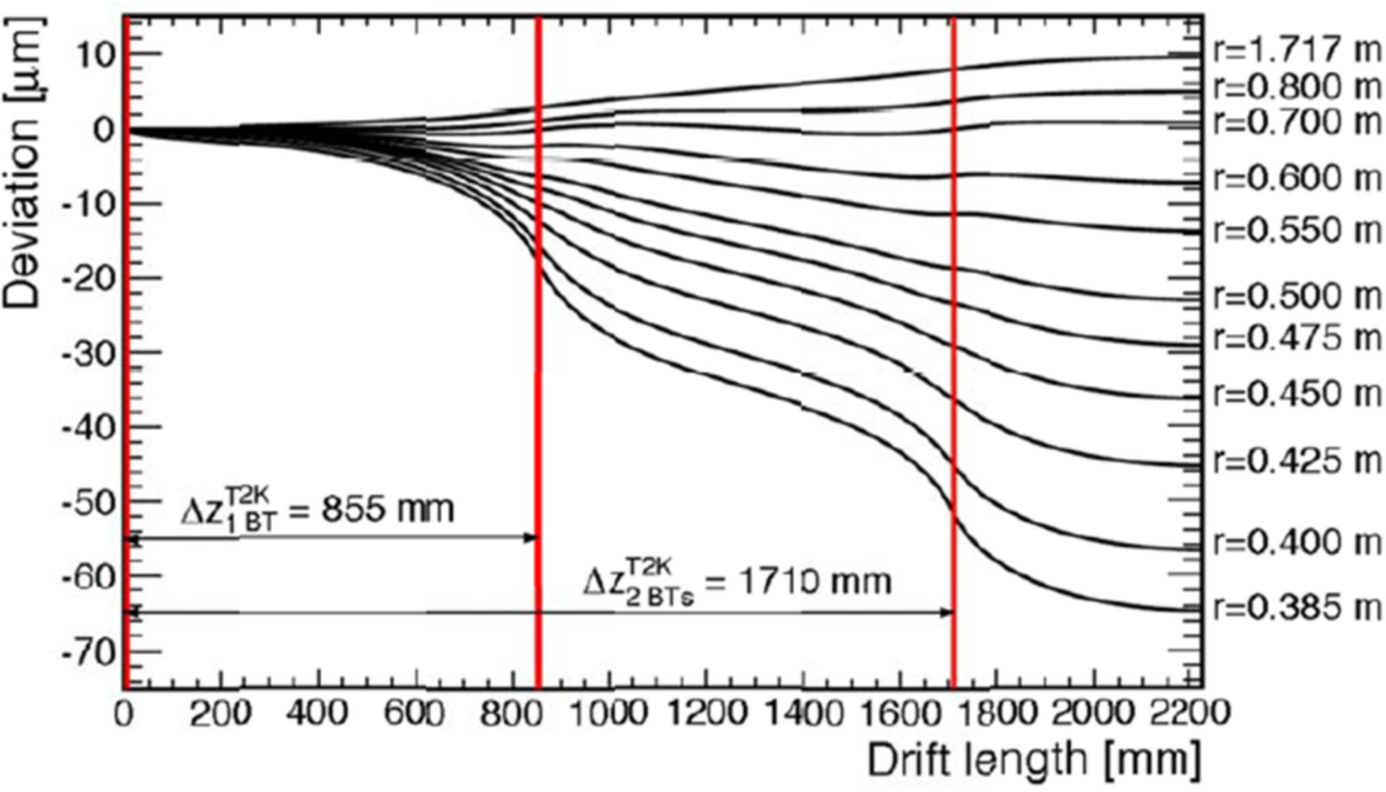
\includegraphics[width=.7\textwidth]{Tracker/TPC_Bonn/plots/TPC-Gate_Fig1gating.pdf}%
\caption{\label{Fig1gating} {Displacement due to the positive-ion discs.}}
\end{figure}

In  Fig.~\ref{Fig1gating} it is assumed that for every drift electron one positive ion drifts back.
The actual amount of displacement should therefore be multiplied by the ratio of the gas amplification
factor to the suppression factor of the ion backflow of the MPGD system. Since the suppression factor by the
MPGD system has been measured to be in the order of order 10$^{-3}$ at
best \cite{Fujii_IonEffects}, the ratio will be larger than one for a gas gain of a few thousand, and distortions larger
than \SI{60}{\micro m} in some parts of TPC would be expected.

At the ILC a TPC point resolution of \SI{100}{\micro m} or better is required by the physics. Thus it is
necessary to either install an efficient gating device to block the ions from the gas amplification, or to correct
the track distortion. Because the machine backgrounds at ILC may not be stable enough to make a reliable
correction possible, an efficient gating device will be needed. Fortunately the bunch-train configuration of ILC
has an ideal time structure for ion gating. The positive ions drift back around \SI{5}{mm} during
the \SI{1}{ms} bunch-crossing period, and can be absorbed by the ion gate which is `closed' (explanation
below) during next \SI{200}{ms} between the bunch trains.

For the expected particle density at ILC, the track distortion by the
{\em{primary}} ions produced in the LCTPC volume is small and has negligible effect.

\subsection{Engineering Challenges: a Wire Gate or a GEM Gate}

Ion gates used for TPCs in past collider experiments consisted of a wire grid. The operation and
structure of the wire gate is well known and can be used for the LCTPC. Figure~\ref{Fig2gating} shows
a simple mechanical prototype of such a wire gate mounted on an Asian GEM module.

\begin{figure}
\begin{center}
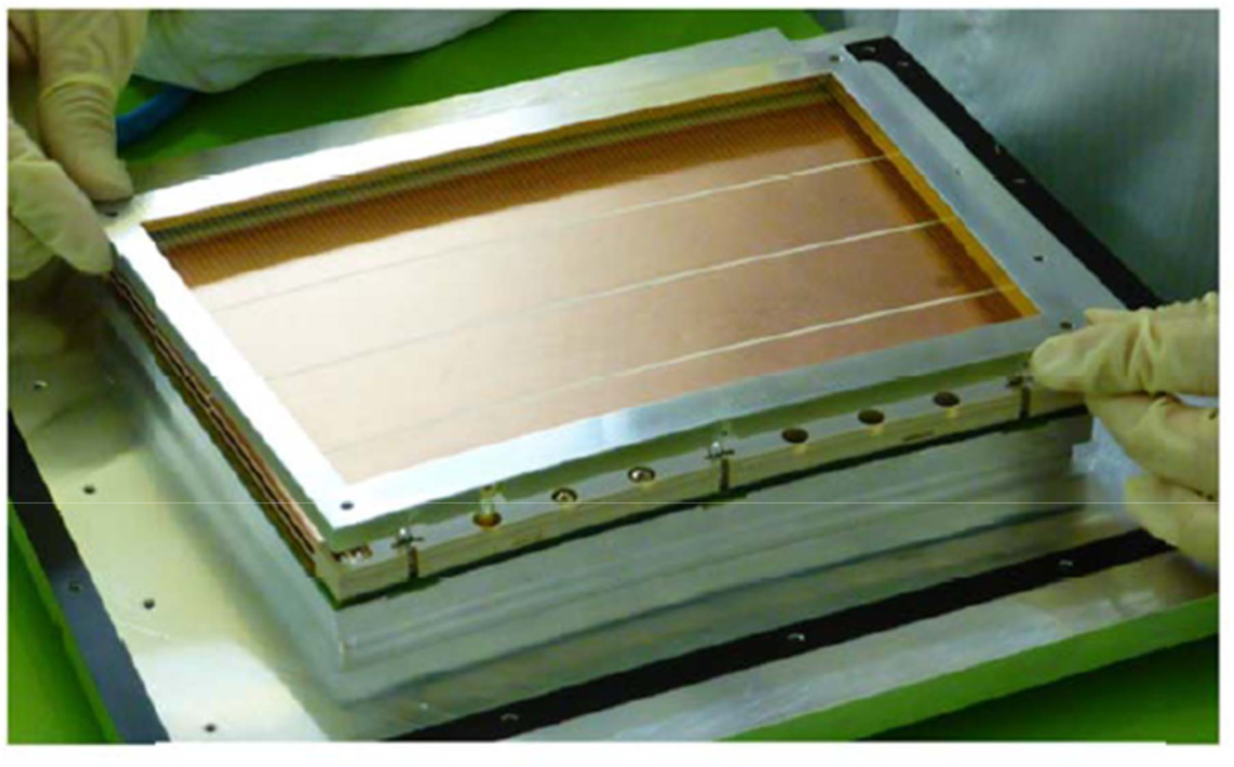
\includegraphics[width=.7\textwidth]{Tracker/TPC_Bonn/plots/TPC-Gate_Fig2gating.pdf}%
\caption{\label{Fig2gating} {Prototype wire gate installed on the Asian GEM module.}}
\end{center}
\end{figure}

The disadvantage of a wire gate for the LCTPC module is to deteriorate the advantages of an MPGD TPC:
the material and space budgets are increased because of the mechanical structure needed to support the many
stretched wires on the module. Therefore, the wire gate is kept as a backup option for the LCTPC, and efforts
are focused on the development of the gate using a GEM foil.

The idea of the GEM gate was proposed by F.~Sauli in 2006 \cite{Sauli2006269}.
The ions from the gas amplification have to be absorbed by the electrode of the gate-GEM in the gate-closed condition.
`Closed' is where the electric field across the gate-GEM is reversed by changing the potential of the bottom
electrode of the gate by about \SI{10}{V}. In the gate-open condition the drift electrons need to reach
to the gas amplification region with a high efficiency in order to not deteriorate the LCTPC resolution
due to loss of signal.

Details of the simulation of GEM gate using the Garfield++ may be found in \cite{LC-DET-2012-079}. Experience was that it is easy
to stop the ions with the necessary suppression factor of 10$^{-4}$ or smaller. On the other hand, it is more
of a challenge to keep a very high efficiency of the drift electrons passing through the gate-GEM in the gate-open
condition. This is because the efficiency is limited by the optical transparency of the gate-GEM when a TPC
is used in a high magnetic field (as in the \SI{3.5}{T} field of ILD) and with a high-$\omega\tau$ gas mixture,
such as the T2K gas \cite{Behnke:2013lya,ref4T2Kgas_ishikawa,Kobayashi201137,Kobayashi2013122} foreseen for the LCTPC. In this condition the drift electron tends to follow the
magnetic field lines rather than the electric field lines, which makes the optical transparency an important parameter .

The first GEM gate prototype for the Asian GEM module for the TPC large prototype (LP) beam test at
DESY in 2009 was \SI{14}{\micro m} thick with the round GEM holes of
\SI{90}{\micro m} diameter and \SI{140}{\micro m} pitch. It had a maximum electron
transmission of 50\% in the magnetic fields of \SI{1}{T} and \SI{0}{T}. It was clear that a GEM
with bigger holes and a narrow rim was needed, that is with larger optical transparency. Simulations found that
GEM holes of the honeycomb shape with very thin rims would maximize the optical transparency.

\begin{figure}
\begin{center}
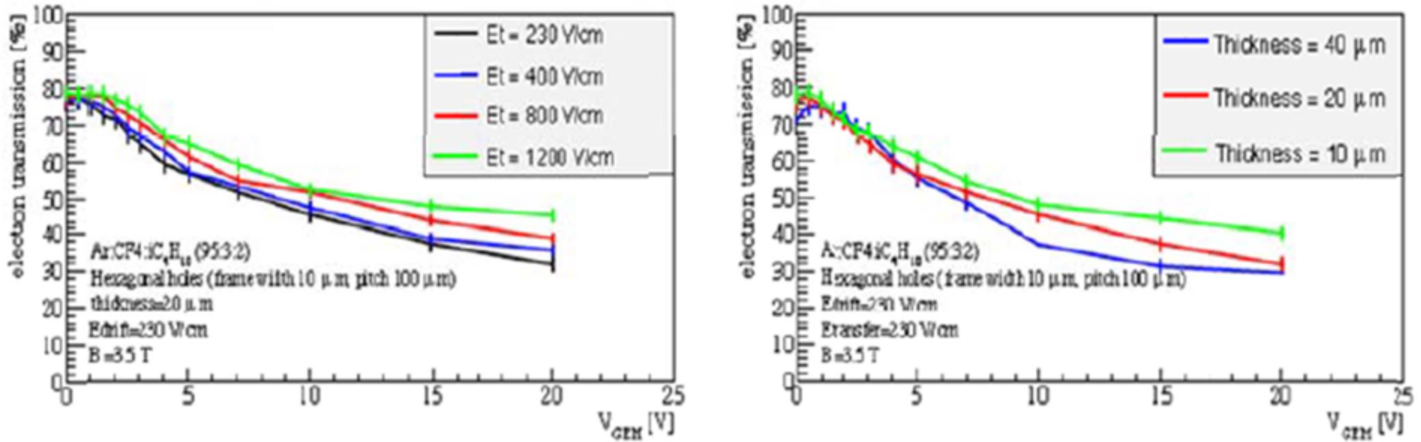
\includegraphics[width=.7\textwidth]{Tracker/TPC_Bonn/plots/TPC-Gate_Fig3gating.pdf}%
\caption{\label{Fig3gating} {The electron transmission simulated for a gate-GEM with the honeycomb-shaped holes of pitch \SI{100}{\micro m} and rim width \SI{10}{\micro m}.}}
\end{center}
\end{figure}

As is seen the simulation results shown in Fig.~\ref{Fig3gating}, the thin gate GEM with
honey\-comb-shaped holes of \SI{100}{\micro m} pitch and \SI{10}{\micro m} rim width is shown to reach
an electron transmission of 80\%. However, a rim width of \SI{10}{\micro m} turns out to be very difficult to produce;
an alternative is presented in the next subsection.

\subsection{Recent Milestones}

In 2013 the Japanese LCTPC group started the actual fabrication of the GEM gate with the large
optical transmission. With the limitations of the available processes of GEM, the specifications
were set using  Fig.~\ref{Fig45gating}(lower)
which are summarized in the Table 1. The target is to fabricate a gate GEM with  honeycomb shape holes
of around \SI{300}{\micro m} diameter and  rim-width of \SI{35}{\micro m} or smaller. The immediate goal
of this study is to test the Asian LP module with this GEM gate in the DESY test beam in 2016.

\begin{table}
\begin{center}
\begin{tabular}{|l|l|}
\hline
Item & Specification \\%$\sim$
\hline
\hline
Optical aperture ratio &  80\% \\
Hole size       & \SI{300}{\micro m}\\
Hole pitch       & \SI{335}{\micro m}\\
Rim size            & \SI{35}{\micro m}  \\
Insulator thickness  & \SI{25}{\micro m}\\
Foil size            & $170\times\SI{220}{mm}$ \\
\hline
\end{tabular}
\caption{\label{gatespecs} Specification of the gate-GEM in the current study.}
\end{center}
\end{table}

Prior to the fabrication of a large, module-sized gate, many small samples of
\SI{10}{cm} $\times$ \SI{10}{cm} were produced to test different processing techniques.
Although some samples by the standard single-mask chemical process were promising, limited resources required that
a major effort be continued with Fujikura Ltd.~\cite{ref5fujikuraltd} using their laser-chemical hybrid technology to produce
FPCs (flexible printed circuits). Details of the Fujikura process for the gate-GEM were presented at MPGD2015 \cite{MPGD2015_gate}.
Figure~\ref{Fig45gating}(upper) shows the structure of one of the gate-GEM small samples made by Fujikura
according to the specifications in Table \ref{gatespecs}.

\begin{figure}
\begin{center}
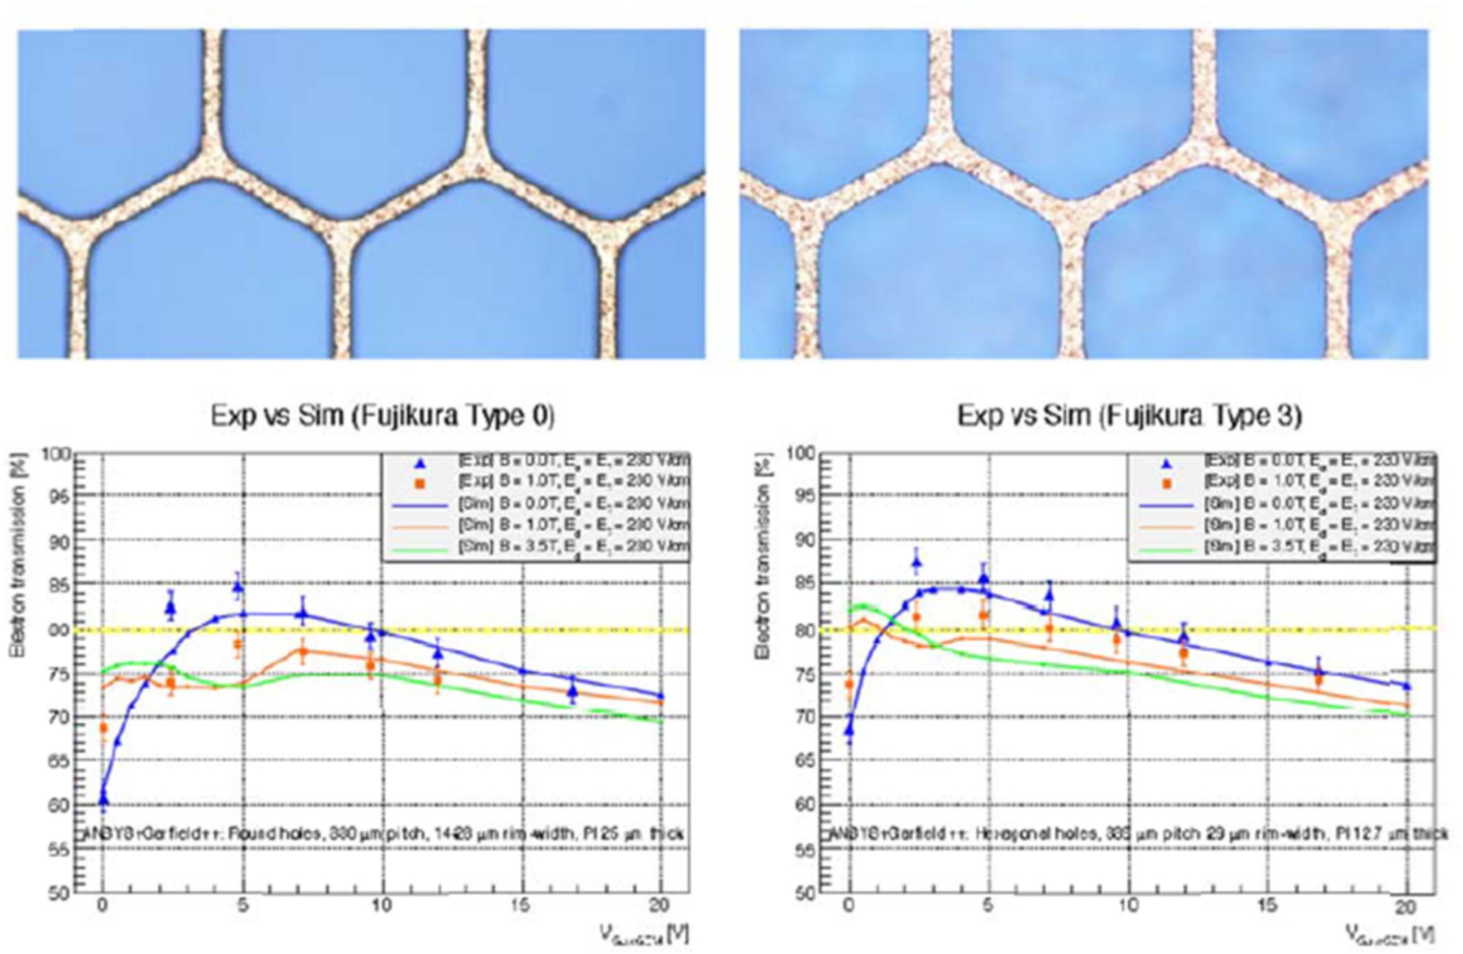
\includegraphics[width=.7\textwidth]{Tracker/TPC_Bonn/plots/TPC-Gate_Fig45gating.pdf}%
\caption{\label{Fig45gating} {Upper: Honeycomb hole structure of the gate-GEM.
The pitch of the holes is \SI{335}{\micro m}, the rim width \SI{29}{\micro m}.
The polyimide insulator is \SI{12.7}{\micro m} thick.
Lower: Preliminary results of the electron transmission measurement are compared to simulation
as functions of the GEM voltage for two types of gate-GEMs. In the left panel are
results for gate-GEM with round holes; in the right panel results for the gate-GEM with the honeycomb-shaped holes.}}
\end{center}
\end{figure}

The electron transmission was measured for these samples, and
Fig.~\ref{Fig45gating}(lower) shows the results of the measurement compared to the simulation in magnetic fields
of 0, 1 and \SI{3.5}{T}. In the left panel, the results for the sample with round holes, and in the right panel
for the sample with honeycomb-shaped holes.  The electron transmissions at 0 and \SI{1}{T} were confirmed
to be better than 80\% while the optical transmission was calculated to be 82\% for the honeycomb-shaped-hole sample.

Having established the best configuration and the best process for the gate GEM with the small samples,
the focus has now moved to the fabrication of the gate-GEM with  the size of the Asian GEM module (Fig.~\ref{Fig6gating}).
Here the major issue for the fabrication is to minimize any defects in the electrode circuit of the gate-GEM
so that there is 100\% stopping power of the ions.

\begin{figure}
\begin{center}
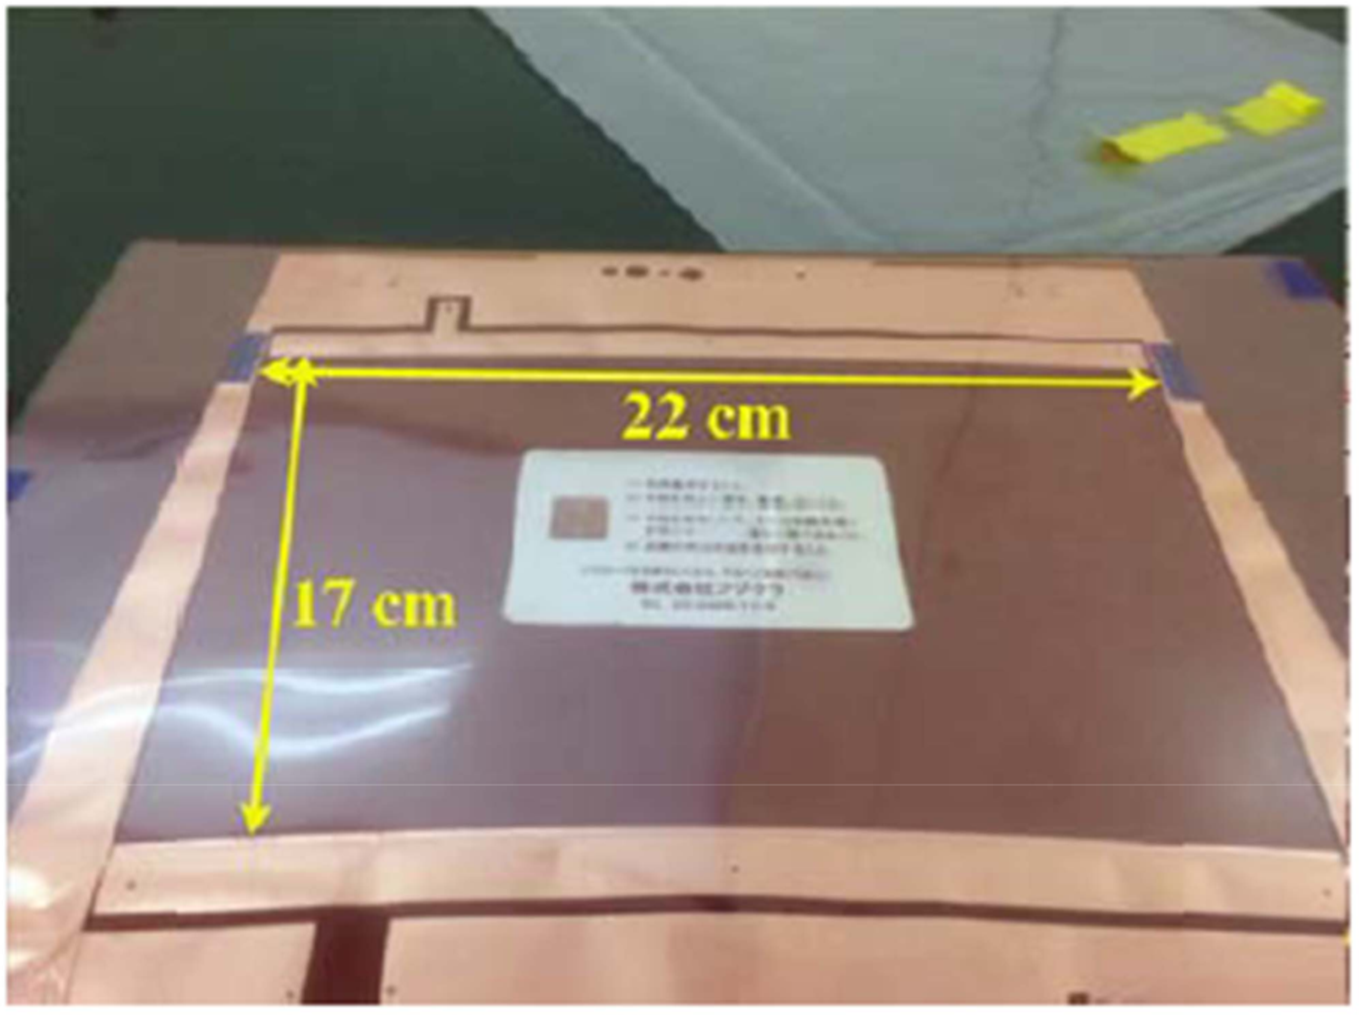
\includegraphics[width=.7\textwidth]{Tracker/TPC_Bonn/plots/TPC-Gate_Fig6gating.pdf}%
\caption{\label{Fig6gating} {A sample gate-GEM for the Asian module.}}
\end{center}
\end{figure}

\begin{figure}
\begin{center}
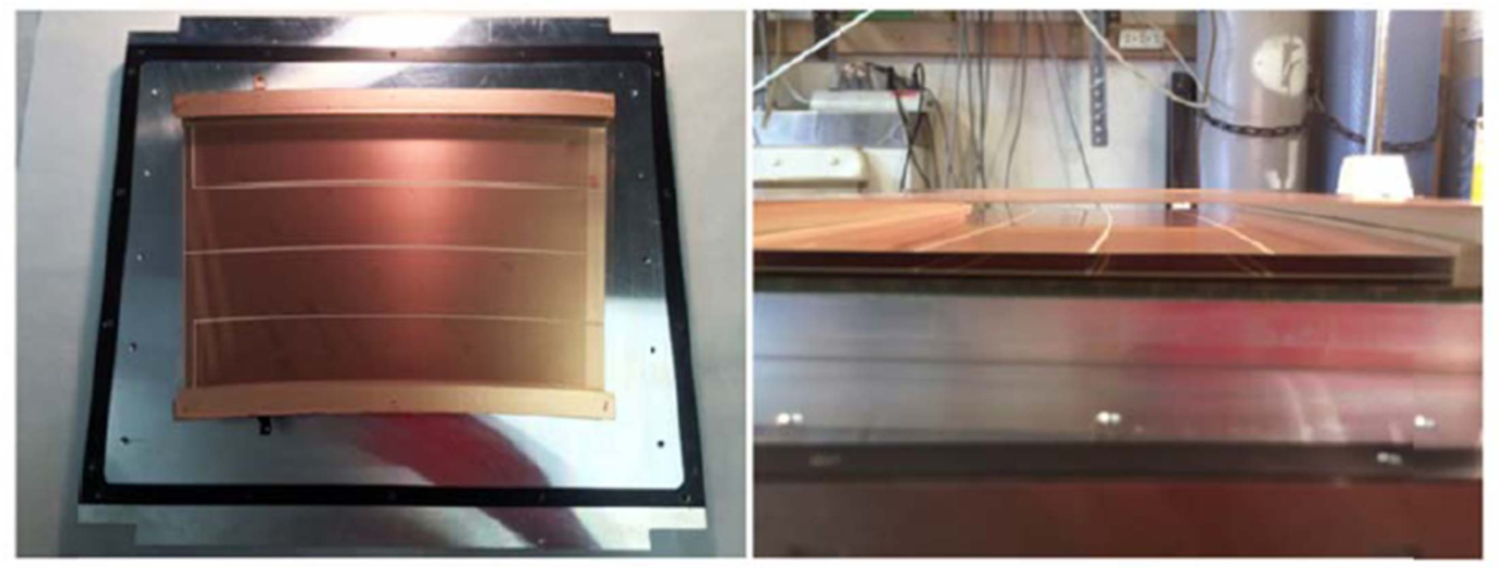
\includegraphics[width=.7\textwidth]{Tracker/TPC_Bonn/plots/TPC-Gate_Fig78gating.pdf}%
\caption{\label{Fig78gating} {Left panel: Test mounting of the gate-GEM. Right panel: Test assembly of the gate GEM on the Asian GEM module.}}
\end{center}
\end{figure}

Figure~\ref{Fig78gating}(left) shows the test mounting of the gate-GEM on the module. As can be seen,
the pattern of the amplifier GEM below the thin gate-GEM can be seen clearly, indicating a  high optical transparency.
Figure~\ref{Fig78gating}(right) is a picture of a test assembly of the gate-GEM on the module.

\subsection{Future Plans}

The production process for the large gate-GEM has been essentially established,
and a few of the good samples for the Asian GEM module have been delivered for testing.
The preparations for measuring the electron transmission by using a laser beam are under way.
Although the Asian model is designed to have a GEM gate mounted on it,
there may be more issues coming up, and some optimization of the mounting method and the module structure
might become necessary for the design of the LCTPC. Beside some difficulties to stretch such a thin
GEM stably, some consideration on the possible ion leak through the module boundaries
for the Asian GEM modules may be needed.

\section{Electronics, DAQ and Cooling}
\label{chap:TPC_sec:electronics}
Most recent update: 2020-05-12 \\
Contact person: Leif J{\"o}nsson (email: leif.jonsson@hep.lu.se)

\subsection{Introduction}
The readout electronics for the TPC has to be adapted to the design of the tracking chamber and the beam structure of the collider. The physics goals of the ILC requires high momentum resolution and two-track separation, which drive the track reconstruction in the $r\text{-}\varphi$-plane to pad sizes of small dimensions. For the $r\text{-}z$-plane a short shaping time and a high sampling rate is necessary to provide the best possible timing information. However, at the same time the noise level has to be kept at a manageable level. The sampling depth has to match the sampling frequency in order to cover the full drift length. The front end electronics has to be accommodated within pad modules, with a channel occupancy that is smaller than the pad size to allow space for the mounting frame, the voltage supply and the cooling system.

The power consumption of the front-end electronics should be kept low such that the heat dissipation does not lead to a temperature increase in the TPC-gas of more than typically \SI{1}{\degreeCelsius} after cooling. In this respect, power pulsing, where the front-end electronics is switched off for about \SI{199}{ms} between the bunch trains, helps significantly.

The readout electronics presently under development aims to demonstrate that the channel occupancy can be made compatible with the small pad size foreseen. It is based on the CERN SALTRO16-chip (shown in Figure~\ref{fig:TPC:SaltroPic}), which integrates the analogue and digital signal processing of the incoming signals within the same compact circuit. Feasibility studies of the readout concept has to be performed with existing ASICs. This prototype system is described below. A final dedicated ASIC for the ILD TPC will have a much larger channel density and higher degree of integration of functionalities and will thus occupy less space than the present prototype electronics. The size of the die is $8.7 \times \SI{6.2}{mm^2}$ and it contains 16 readout channels. The chip is programmable with respect to gain, rise time, decay time and polarity. The sampling can be clocked at frequencies 5, 10, 20 and \SI{40}{MHz} and it allows for power pulsing.

\begin{figure}
    \centering
    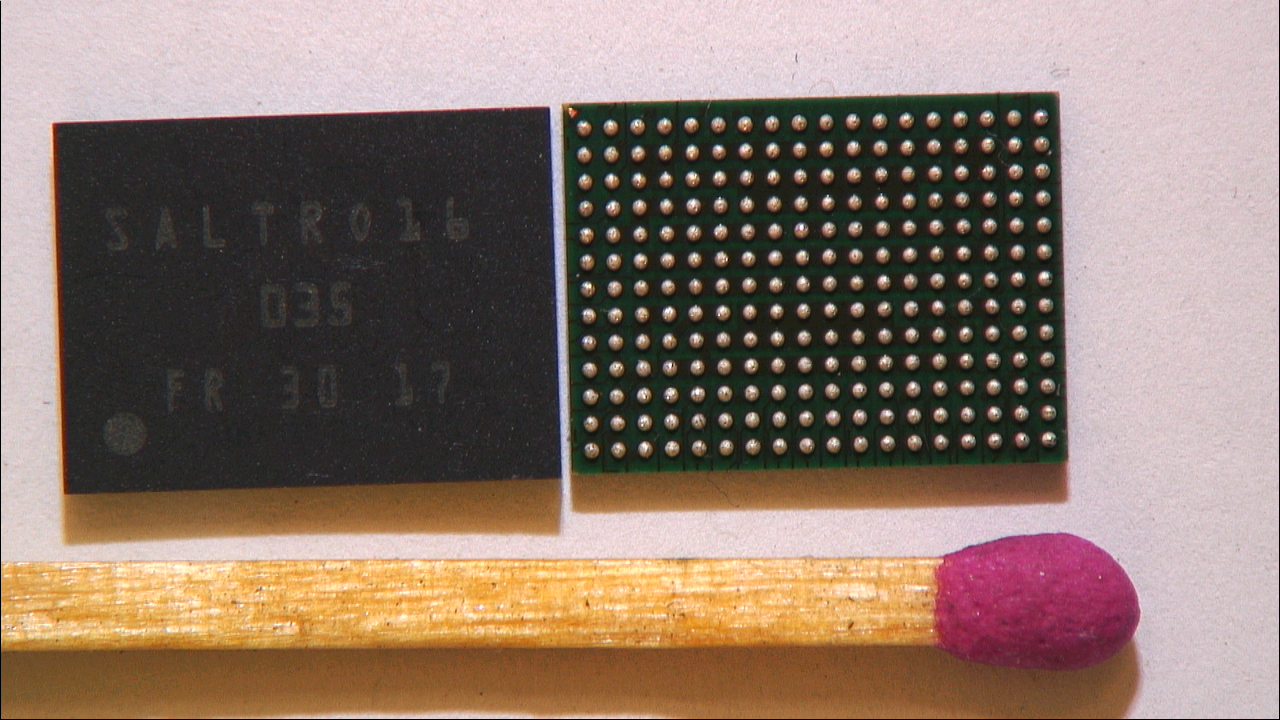
\includegraphics[width=.5\linewidth]{Tracker/TPC_Bonn/plots/TPC-Electronics_JonssonsALTRO_Chip-Photo_07062018}
    \caption{Photograph of two SALTRO-16 chip side-by-side and a matchstick for comparison.}
    \label{fig:TPC:SaltroPic}
\end{figure}

In total 840 untested dies have been obtained and delivered to the company, which performs the packaging into small capsules of size $12\times\SI{9}{mm^2}$. The bottom side of the chip contains small tin balls organized in a BGA pattern for soldering of the packaged SALTRO16 chip on so-called Multi-Chip Modules (MCM).

Eight SALTRO16 chips are mounted on an MCM, which also contains a CPLD (Complex Programmable Logic Device) controlling the data flow. The MCM-board is the smallest unit in the front end electronics and it is attached to the pad plane via four micro-connectors, whereas on the opposite side of the board there are two connectors, via which the low voltage is distributed and the signals are transmitted. The MCM-board is designed in High Density Interconnect (HDI) technology, by which the number of layers is significantly reduced compared to conventional PCB design. The dimensions of the MCM-board are $32.5 \times \SI{25}{mm^2}$ and serves 128 readout channels. This corresponds to a channel occupancy of about $\SI{6.4}{mm^{2}}$, although some space is also required for the high voltage connectors of the gas amplification system (GEMs and Micromegas) and the cooling system.

A serial readout system is used for the signal transfer to the DAQ computer. The MCM-board and the Scalable Readout Unit~\cite{1748-0221-8-03-C03015} (SRU) communicate directly via the Data Trigger Control (DTC) link. Communication, data transfer and control, between the SRU and a DAQ computer is done via Ethernet.

Cooling of the front end electronics is a challenge since the size of the cooling system must match the smallness of the electronics and still provide efficient cooling. The total power consumption of an MCM-board in continuous operation
is \SI{3203}{mW} on the top side and \SI{3028}{mW} on the bottom side. In power pulsing mode, with a bunch train of \SI{725}{\micro \second}, containing 1312 bunches, the power dissipation is reduced to about \SI{223}{mW} per MCM-board on the top side and \SI{48}{mW} on the bottom side. A cooling system with cooling pipes that run on top of the MCM-boards, using two-phase \ce{CO2} coolant, is considered. Another possibility would be to use micro-channel cooling, which has been developed by the semiconductor community. Such systems are presently further developed within the AIDA2020 project, for applications in high energy physics experiments. The ILC cycle is not realistic in a test beam environment as at e.g. DESY. To get a reasonable trigger rate is e.g. a cycle with \SI{5}{ms} beam at \SI{10}{Hz} more useful, which corresponds to \SI{343}{mW} per MCM-board on the top side and \SI{168}{mW} on the bottom side, in power pulsing mode.

\subsection{Recent Milestones}
A system for testing the SALTRO-16 chips has been built and debugged. We are aiming at a readout system with at least 10,000 channels, which requires a yield of about 75\%. The tests of two pre-series have been completed. The first one, containing 34 chips, gave a lower yield, requiring an improved bonding procedure. The second pre-series, containing 55 chips, gave a yield well above the goal and we decided to go ahead with the full production.
The delivery of the bulk of the chips happened at the end of the year 2018.
The design of the final 16-layer MCM-board was completed and the boards were manufactured. By pushing the boundaries of commercially available assembly techniques to the limit, read-out of sensor pads, as small as \SI{6.3}{\milli\meter\squared}, could be achieved with the MCM-board connected parallel to the pad plane. We have simplified the design by reducing the number of separate voltage levels needed from seven to two. Initial tests revealed some bugs in the PCB design, most of which could be fixed. Prior to the performance tests of the MCM-board, a prototype LV board, providing low voltage supply for a single MCM-board, was designed and produced. The design of the final LV-board intended for five MCM-boards is well under way.
For tests of the performance, two MCM-boards were mounted by the DESY electronics group at the end of 2019. The tests showed that data could be read and written and thus the concept was proven to work. Pedestal runs were performed and gave good results, and the noise performance was promising. However, this first prototype of the readout board required some corrections, which have been implemented and the next version of the MCM PCB has been ordered. The official delivery time was 8.5.2020, but at the time of writing the supplier claims a delay of about one week. The assembly by the DESY electronics group will follow together with further tests.

\subsection{Engineering Challenges}
The final aim is to produce front end electronics, high voltage supply and a cooling system which are compatible with a pad size of $1 \times \SI{6}{\milli\meter\squared}$. The compactness of the electronics and the space limitations are major challenges, as well as designing a suitable and efficient cooling system. An elegant solution for the low voltage supply has to be found and due to space limitations the design of the mechanical support for the electronics is also a challenge.

\subsection{Future Plans}
In case the upcoming tests are successful, a fully mounted MCM-board will be produced and tested.
Until we have got help with the FPGA-programing we will not be able to test the rest of the chips and
thus no further MCM-boards can be produced.
The design of the micro-channel cooling support structure is ready and production is planned.

\section{Mechanics and Calibration}\label{chap:TPC_sec:mechanics}
Most recent update: 2016-03-28\\
Contact person: Ties Behnke (email: ties.behnke@desy.de)\\

\subsection{Introduction}
A key component of the TPC at a future collider will be the design and construction of the field cage. The cage should be light weight, yet mechanically and electrically stable. It should provide support for the cathode and the anode systems, and allow excellent field shaping in between.
To test the concept for such a field cage a prototype has been built as part of the LCTPC test infrastructure \cite{1748-0221-5-10-P10011}. The field cage is made from a light weight composite sandwich structure. The mechanical structure is given by a honeycomb layer, which is covered on the inside and the outside by a glass fibre reinforced epoxy layer. On the inside a Kapton foil provides electrical insulation, and field shaping through a system of copper ring electrodes. On the outside a thin aluminum layer provides grounding. Integrated into the field cage a laser based calibration system is foreseen.

The prototype field cage has been constructed in 2008 and has been used with all different readout technologies since. It is equipped with an aluminum based endplate, which can host up to seven identical readout modules. It is designed to fit into the PCMAG magnet \cite{Yamamoto199475} infrastructure, which is installed at the DESY test beam facility \cite{DESY2TB}.

%Another challenge is the development of a compact and efficient cooling strategy. Currently, CO$_2$ based systems are favoured and are being prototyped.

A large system like the TPC poses particular challenges to calibrate the system and to maintain the calibration. Currently several systems are under consideration.

An important part of the calibration will be done based on data recorded, without special hardware. Tracks will be used to align the different modules relative to each other, and to measure and correct field distortions.

While tracks are an excellent method to derive relative corrections, and to equalise the response, it might be difficult to reach the ultimate absolute resolution without an external unbiased reference. This reference can come from different sources. Within the ILD detector design silicon detectors are foreseen before and after the TPC, which will provide an external reference. These systems can be used to calibrate the field distortions, and to set the scale for the momentum measurement. Another system will be based on laser beams. Laser beams will be used in two ways. Well focused small cross section beams can be inserted into the drift volume, and serve as fake tracks. The ionization along the laser beams is recorded as for normal tracks, and can be used to calibrate the response of the TPC. A wide laser beam can be used to illuminate the cathode of the TPC. Dots or lines of a low work-function material like e.g.~aluminium on the surface of the cathode would then provide well defined spots where the laser
light can liberate electrons. These electrons then drift towards the anode and sample any inhomogeneities on their way. Thus, they can be used to monitor and ---to some extent--- determine the field properties inside the drift volume. Both types of laser beams need to be inserted into the TPC, and will require the design and implementation of sophisticated hardware.

% %\subsection{Recent Milestones}
\subsubsection{Engineering Challenges}
The current field cage has been successfully used in numerous test beam campaigns. However, it has failed to deliver the ultimate mechanical precision which is needed for the demonstration of the anticipated momentum resolution of the TPC system. In particular, the manufacturer has failed to deliver the needed alignment between the anode and the cathode, and has introduced a small overall skew into the field cage. The main challenge will be to develop and build a second generation field cage which fulfills the precision requirements. For this an entirely new tooling is being developed, which should help to ensure the mechanical precision.

The results from this prototype field cage will then be applied to a study of the design of the full field cage for the ILD TPC. A central and so far unsolved engineering challenge is the support of the TPC in the overall detector. Here a combination of light weight, space saving support structures combined with superb mechanical stiffness need to be found. Particular attention will also need to be payed to the behaviour of the system in case of earth quakes, given that the proposed site of the ILC in Japan is located in an earth-quake prone region.

An open and as yet unsolved issue is the design of the central cathode of the TPC. This system is located in the centre of the detector, very difficult to access. It needs to be light weight, yet dimensionally very stable. It will be supplied with high voltage of close to \SI{100}{kV}. The supply of this very high potential in a safe and reliable way is under study and represents significant challenges.

As described above laser beams will be used to calibrate the system. The insertion and guidance of these laser beams present significant challenges. Ways will need to be found to bring the laser beams to the TPC. The laser will have to be installed on the outside of the detector, so that transport ways of several meters through a very crowded environment are needed.

\subsection{Future Plans}
Over the next few years a full engineering design of the ILD TPC will be developed. This will include a detailed simulation of the TPC system, and its mechanical properties, and its integration into the ILD detector as a whole.

Detailed problems which will need to be addressed are:

\begin{itemize}
\item Finite Element Method (FEM) calculations of the field cage and the endplate
\item Optimisation and final decision on the layout of the endplate: size of modules, number of modules, etc.
\item Design of the support system of the TPC in the ILD detector
\item Study of the mechanical properties of the TPC support in view of vibrations and overall stability
\item Design and implementation of a system of laser beams in the TPC drift volume
\item Design and implementation of a system to illuminate the TPC cathode with a laser beam.
\end{itemize}

%Contributing : DESY, KEK, U Cornell, U Hamburg, CEA Saclay, Nikhef, U Victoria

%\subsection{Recent Milestones}

%The cooling system of the PCMAG has been modified from cooling with liquid helium to a system using a closed helium circuit with external compressors and cold heads installed in the PCMAG. This allows a continuous operation over long time periods of several months and improves the usability and safety of the setup.

%Contributing: AIDA, KEK, DESY

%A two-phase CO$_2$ cooling system (TRACI) has been installed at the test beam area and successfully operated at two test beam periods, so far.

%Contributing: KEK, DESY, Nikhef, CEA Saclay
%
%
%\subsection{Engineering Challenges}
%
%The field cage of the LPTPC has to be mechanically and electrically stable, while keeping the material budget of its wall structure at about 1\% of X$_0$. Its mechanical tolerances are very tight to ensure an electric field homogeneity of $10^{-4}$.
%
%\subsection{Future Plans}
%
%The first field cage of the LPTPC had been designed at DESY and built by an external company.  The allowed mechanical tolerance of max. $0.5\,\mathrm{mm}$ for the tilt of the cylinder axis was not kept. A new field cage will be constructed in-house at DESY. Material tests and the preparation of the required construction tools are ongoing.


\thispagestyle{empty}
\newgeometry{margin=1.5cm} % modify this if you need even more space
\begin{landscape}
    \centering
    \begin{adjustbox}{max width=1.1\textwidth,totalheight=1\textheight}
\begin{tabularx}{2\textheight}{lXXXX}
    \toprule
    R\&D Technology & Participating Institutes & Description / Concept & Milestones & Future Activities \\
    \midrule
        Asian GEM &
        Saga, KEK, Hiroshima, \newline Kindai, Kogakuin, Iwate, \newline
    Nagasaki IAS, Tsinghua &Design of an endcap readout module with a stack of
    two thicker laser etched polymer-based GEMs and pads  & 2010-2013: Several
    test beam campaigns were performed with three readout modules. & During test beam activities the stability of the HV was not
as good as in lab tests. The origin of the discharges is being
investigated. A modified module with a gating device will be
designed and constructed in the next step, and pad
plane adapted for the SALTRO is also planned. (2016/17) \\
    \midrule
        GEM &
        DESY, Hamburg \newline Bonn \newline Siegen &
        Design of an endcap readout module with a stack
of three standard CERN GEMs and pads&2009-2013: Several test beam campaigns were performed with
three readout modules.

 &Though no problems occurred during the test beam, the
HV-stability is still being investigated. A new module with
gating device, reduced local field distortions and pad
plane adapted for the SALTRO is planned. (2016/17)\\
    \midrule
       Resistive Micromegas &
       CEA Saclay, Carleton &
       Design of an endcap readout module with a Micromegas gas amplification
       stage, a resistive layer for charge dispersion and integrated readout.
       Construction of 11 modules.&
       2010-2015: Several test beam campaigns were performed with up to seven
       readout modules, covering the complete LP-endplate. &
       New materials as resistive layer are being investigated. A module with lower local field distortions is planned.\\
    \midrule
       GridPix Concept \newline GEM + pixel readout &
       Bonn, NIKHEF, CEA Saclay \newline Bonn, Siegen &
       Design of an endcap readout module with a highly pixelized readout with
       GridPixes. These devices consist of a Micromegas mesh built by
       postprocessing technology on a pixel ASIC. Alternatively a GEM-stack is
       used as a gas amplification stage.&
       2009-2015: Several test beam campaigns with up to three modules were
       performed. The three modules featured a total of 160 GridPixes and this
       test beam was performed in March/April 2015. This demonstrated that a
       large area could be covered with GridPixes and about 100 GridPixes per module could be operated.&
       2017: The successor chip Timepix3 will be implemented in the readout chain and
       a test beam with several Timepix-3 chips is planned. This new chips
       fulfills basic requirements for an operation in an ILD environment.\\
    \midrule
        Field cage &
        DESY &
        Design and construction of a TPC field cage &
        2009: A first prototype has been built and is used as a test device at
        DESY &
        A new field cage with improved geometrical precision is
        under construction at DESY. (2017)\\
    \midrule
        Electronics &
        Lund, CERN, CEA Saclay &
        Design of a readout electronics fit for test beam
        operation at T24/1 at DESY and for investigation the
        requirements of the ILD-TPC electronics.&
        2009: Sofar, readout systems based on the AFTER and the
        ALTRO chip have been used with 10,000 channels each.&
        A new system based on the SALTRO-16 chip is being prepared
        (2017). Simulations on the impact of key electronics parameters on the
        TPC-performance are planned.\\
    \midrule
        DAQ &
        Lund, ULB-VUB, Hubei &
        Design of a data acquisition system fit for test beam operation at
        T24/1 at DESY. &
        Sofar, DAQ systems for both readout systems (AFTER and ALTRO) have been set up. &
        A new DAQ system for the SALTRO-16 based readout electronics  is being
        prepared and will be available soon.\\
    \midrule
        Endcap &
        Cornell &
        Study of different endplate designs for an ILD-TPC with
CAD programs and production of smaller endplates fit
for operation at test setup at T24/1 at DESY. &
A detailed model of the endplate was implemented in a
CAD program and in 2009 a first endcap for the test beam
setup has been produced several years ago. A new
version also fulfills the requirements of the material
budget and will be used from 2015 onwards.&
Simulations optimizing the module size are planned.\\
    \midrule
        &
         CEA Saclay, DESY &
        Mechanical studies for ILD-TPC regarding the effect of
pressure, weight, hanging/support schemes on the
mechanical deformation of the endplate and field cage. &
 First studies have been done.
&
 More detailed studies are planned\\
    \midrule
        Calibration &
        BNL, CERN, Indiana, Kolkata &
        Laser calibration system, Alignment/calibration of the TPC, Integration with other tracking systems & & \\
    \midrule
        Study of systematic effects &
        Victoria, Kolkata &
        Field distortions are a major source uncertainties in track
        reconstruction. The sources of these distortions are studied and minimized. & & \\
    \midrule
        Analysis software &
        DESY, Carleton, CEA Saclay, KEK, Saga, Siegen, Tsinghua &
        Development of a software package MarlinTPC, which serves all groups
        for reconstructing and analyzing the test beam data and for
        simulation, reconstruction and analysis of ILD events. &
        MarlinTPC is well developed and the key analysis tool for all
        analyses. &
        Further improvements are continually made.\\
    \midrule
        Ion backflow/Gating &
        Japanese Univers., KEK, Tsinghua, Kolkata, DESY &
        The ion back flow from gas amplification stages is a major source for
        time dependent field distortions and has to be suppressed as much as
        possible. With simulations and experimental setups the minimization of
        ion production and the reduction of the back flow by a gating device
        are under study. Field distortions are a major source uncertainties in track
        reconstruction. The sources of these distortions are studied and
        minimized. & Simulations have shown, that all gas amplification stages
release too many ions into the drift volume and a
gating device is necessary. 2014:  A first MPGD-based device,
a Gating-GEM, has been produced and is being
compared to a standard wire gate.
& 2016: module sized GEM-gates will be available.
Then the impact of the gate on the TPC-performance will be
studied by using a UV-laser facility at KEK, and in test
beams.\\
    \midrule
        Cooling &
        KEK, Saga, NIKHEF, Saclay, Kolkata &
        Cooling is important to divert the heat produced by the
readout electronics at the endplate. The temperature
influences the gas gain and drift properties in the
gas and has to be kept as stable as possible to
achieve a reliable measurement. &
2014: A \ce{CO2} cooling plant has been purchased and setup at the
test beam site. First results show a significantly reduced
temperature gradient due to heating at the endplate.
& Cooling of the SALTRO-16 based module will be studied
with a mockup which emulates heat and mechanical
conditions of the module. Then, the SALTRO-16 based
module will be built with the \ce{CO2} cooling pipes.\\
    \bottomrule
\end{tabularx}
\end{adjustbox}
\end{landscape}
\restoregeometry

\chapter{Calorimeters}
\section{Motivation and Constraints for Calorimetry at Linear Colliders}

The design of Linear Collider experiments is fundamentally influenced by the requirement for excellent jet energy resolution. The goal of being able to reconstruct hadronic \PZ events with a resolution comparable to the intrinsic width translates to a requirement on the jet energy resolution of $3.5\%-5\%$.

Linear Collider Detector concepts are designed for particle flow, which exploits the fact that approximately 60\% of the energy in a typical jet is in the form of charged tracks, 30\% is in form of photons, and 10\% occurs as neutral hadrons. With the tracking detectors having the best energy resolution, and hadronic calorimeters having the lowest, the jet reconstruction performance depends crucially on being able to separate the different components of a jet. To reduce energy loss in insensitive material, detector concepts at Linear Colliders are designed with calorimeters inside the solenoid. This requires the absorber material to have a very short interaction length to contain the shower.

Highly granular calorimeter concepts consist of segmented absorber stacks interspersed with measurement layers, with a segmentation of $\approx 10\text{mm}^2$ in the electromagnetic calorimeter and a few $\text{cm}^2$ in the hadronic calorimeter. Digital readout requires an order of magnitude smaller segmentation and is also being studied. These calorimeters aim at separating the showers of individual particles in situ, and at matching the detector signatures of particles across the main tracker, the electromagnetic calorimeter, and the hadronic calorimeter. Their performance relies in principle on the ability to identify and subtract the contributions of charged hadrons from the calorimeters.

Dual-readout calorimeters, on the other hand, are classic fully absorbing calorimeters that measure particle energy losses within defined volumes. The preferred structure from the RD52 studies\footnote{\url{http://www.phys.ttu.edu/~dream/}} is a copper absorber mass with scintillation and \v{C}er\-enk\-ov fibers embedded throughout on a spatial scale of \SIrange{1}{2}{mm}, and the light in the fibers is read out from the rear of the calorimeter enabling complete hermeticity. 

%A recent paper summarizes our current understanding of dual-readout calorimetry \cite{Lee:2017xss}.

\section{Scintillator Strips}
Most recent update: 2015-04-28 \\
Contact person: Tohru Takeshita (email: tohru@shinshu-u.ac.jp)
\subsection{Introduction}

The CALICE scintillator strip-based ECAL (ScECAL) uses a scintillator  strip
structure to deliver the granularity and resolution required of an ILC detector.
Each strip is individually read out by a Multi Pixel Photon Counter (MPPC, a
silicon photon detector produced by Hamamatsu Photonics K\.K\.~\cite{Gomi:2007zz}). Although
plastic scintillators have been widely used in calorimeters, this is the first
time that a highly granular calorimeter has been made using scintillator strips.
Such an ECAL has a smaller cost than alternative technologies using silicon
sensors (e.g.~\cite{1748-0221-3-08-P08001}). The MPPC has promising properties for the ScECAL: a small
size (active area of $1\times\SI{1}{mm^2}$ in a package of $2.4 \times 1.9 \times \SI{0.85}{mm^3}$), excellent
photon counting ability, low cost and low operation voltage ($\SI{70}{V}$), with
disadvantages of temperature-dependent gain, saturation at high light levels,
and the dark noise rate. The use of tungsten absorber material
minimises the Moliere radius of the calorimeter, an important aspect for the
effective separation of particle showers required by PFA reconstruction. The
chosen strip geometry allows a reduction in the number of readout channels,
while maintaining an effective granularity given by the strip width, by the use
of appropriate reconstruction algorithms. One such algorithm, know as the Strip
Splitting Algorithm~\cite{Kotera2015}, has been developed and demonstrated to perform well in
jets expected at ILC.

\subsection{Recent Milestones}
\begin{itemize}
	\item introducing a new scintillation light readout scheme, with different scintillator strip shape by having better homogeneity
	\item photo-sensor of increased number of pixels in $\SI{1}{mm}\times\SI{1}{mm}$, this leads larger dynamic range for the calorimeter
	\item more experience on the FE read out board and ASICs
\end{itemize}
They are not published yet, instead some proceedings

\subsection{Engineering Challenges}
\begin{itemize}
	\item wrapping the scintillator strip and align them on the FE read out layer automatically
	\item mass test facility for the read out layer
\end{itemize}

\subsection{Future Plans}
\begin{itemize}
	\item deciding on the scintillator layer: shape of scintillator strip, how to read out scintillation light, the location of  photo-sensor, size and shape of photo-sensor and mass production scheme
	\item developing photo-sensor with Hamamatsu photonics company, to have lager dynamic range and mass test scheme
	\item establish a detector fabrication plan
\end{itemize}

\section{Silicon-Tungsten ECAL in ILD}
Most recent update: 2018-06-04\\
Contact person: Jean-Claude Brient (email: brient@llr.in2p3.fr)
\subsection{Introduction}
The group of the silicon-tungsten electromagnetic calorimeter for ILD aims to develop a highly
granular detector optimized for particle flow measurements. The calorimeter uses a
sandwich architecture of silicon sensors with $5\times \SI{5}{mm^2}$ pixels as active elements embedded in an
alveolar structure made of tungsten and carbon fiber. The group is active in the development of
simulation software and algorithms for calorimeter reconstruction, as well as in the design of readout
chips, front-end electronics boards, mecanical structures, cooling and in ILD
integration.

\subsection{Recent Milestones}
The work is now focusing on the construction of a technological prototype. This
is a new milestone after the successful operation of the ``Physics Prototype'' in the
years 2004--2011, including large scale beam tests at DESY, CERN and FNAL and data
analysis~\cite{1748-0221-3-08-P08001,2009JPhCS.160a2065B,2010JInst...5T5007A,Adloff201197,1748-0221-6-07-P07005}.

In the technological prototype and in the ILD design the front end SKIROC
chips~\cite{1748-0221-6-12-C12040,Amjad201578} are embedded into the calorimeter layers and mounted on
multi-layer printed circuit boards (PCBs). Four silicon sensors are glued with
a conductive epoxy to the readout PCB. Depending on the ILD and the silicon
sensor sizes, up to about ten of these PCBs will be connected together in-line
and read out from one end by a data acquisition (DAQ) electronics. The sandwich
of the silicon sensors with PCBs on both sides of the absorber layer
represents one active module, called ``slab''. It is slided in the tungsten --
carbon fiber alveolar structure. The slab absorber layer is also made of
tungsten wrapped in carbon fiber. In this way, half of the absorber layers are
in the structure and half are in the slabs.

A series of tests with simplified PCBs have been carried out starting from
2012: several beam tests at DESY, cosmic calibrations and infrared laser
tests. Each simplified PCB served one silicon sensor. The power pulsing
operation of the SKIROC chips has been demonstrated. The bias currents of the
chips were shut down and raised with a frequency between \SIrange{1}{20}{Hz}. It was
shown that the SKIROC currents should be switched on at least \SI{600}{\micro \second}
before physical events, so that all transition processes are finished.
Mechanical rigidity of electrical interconnections under changing Lorentz
force and also, the stability of pedestals was checked in the power pulsing
mode in the magnetic fields of up to \SI{2}{T}. The continuous cosmic data taking
during 24 hours allowed to calibrate each pixel with 3\% statistical accuracy.
The variation of cosmic MIP signals across all channels was measured at 3-4\%
level. It was found to be dominated by the spread between the chips and by
the variation of electronic channel gains within a chip. The same spread is
measured by a calibrated charge injection into SKIROC preamplifiers. In
cosmic and test beam data the signal-over-noise ratio for MIP signals was
measured at the level of 8 -- 20. It depended on the SKIROC gain, the better
values were obtained for the gain 5 times higher than nominal.

The infrared laser tests have been used to study the so-called ``square''
events. They are caused by a capacitive coupling (cross-talk) between a
silicon sensor guard ring and its boundary pixels. The guard ring ensures low
dark currents of the sensor under high voltage. For technological reasons it
is not grounded. High local signals at the sensor periphery may, therefore,
propagate to all boundary pixels, fire them and produce ``square''
events. With an improved segmented guard ring design, the cross-talk is
reduced to $\le$0.5\% per outer pixel side, as it was measured with the laser
induced signals. Hamamatsu HPK company also developed a new ``no guard ring''
design, their small sensors demonstrated both the lowest guard ring
cross-talks and sufficiently low dark currents. Another activity which has
been started in 2015, is the study of dark current dependence on neutron
irradiation dose at a nuclear reactor.

Generally, the analysis of accumulated beam test, cosmic and infrared laser
data validated the concept of the front end electronics. It will also allow
for correcting an observed shortcomings of the SKIROC chips and the first
PCB. A new version of PCB serving four sensors as required for ILD, has been
designed and produced, see Figure~\ref{ild_siw_ecal_fev}.
\begin{figure}
\centering
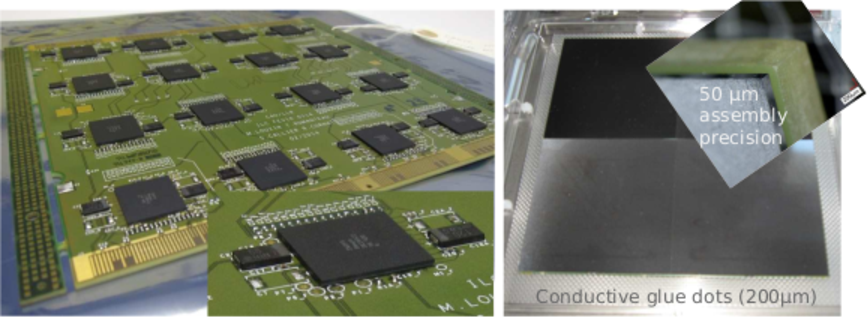
\includegraphics[width=\textwidth]{Calorimeter/SiliconTungstenILD/FEV_gluing_photo.pdf}
\caption{Left: new PCB with 16 SKIROC chips and 1024 channels, right: 4 sensors
 aligned and prepared for robotic gluing to PCB.}
\label{ild_siw_ecal_fev}
\end{figure}
To increase a channel density, a ball grid array
(BGA) packaging of the SKIROC chips was chosen. The gluing of four fragile silicon
sensors with a gap in between of only \SI{100}{\micro\meter} has been successfully
performed with a robot. The first detectors have been assembled in 2015 and
the first tests with the cosmics and the laser have shown a good performance. An assembly
procedure together with quality controls is formalized and well documented.
Further improvement and production of the new version of SKIROC chips is planned
for both ILD and for a CMS phase-2 endcap calorimeter upgrade project
(HGCAL). The combined with HGCAL beam tests at SPS in CERN are planned in
November 2015 and in 2016.

The mechanical design of ILD ECAL is well advanced. A full scale prototype of
a barrel tungsten -- carbon fiber alveolar module with three towers of 15
alveoli has been successfully produced with required tolerances. A full scale
absorber part of the barrel slab has been also manufactured with tungsten
substituted by carbon to reduce the cost. The mechanical simulations of one
alveolus structure have been verified with the measurements using a special
prototype with molded Bragg grating fibers. When elongated under loads, such
fibers change a frequency of reflected light, allowing very precise
measurements. The same technique is used in constructing buildings, bridges
etc. A long \SI{2.5}{m} endcap carbon structure with 3 alveoli is also
successfully produced. The rails supporting ECAL on the HCAL face in ILD, and
also the transport and handling tools for future ECAL assembly have been
designed and mechanically simulated.

Thermal simulations have shown that a passive cooling inside alveoli should be
sufficient. Outside water cooling will be performed with leakless loops, first
prototypes exist.

In addition to the hardware development, there is a big activity on ILD
optimization and on PFA algorithms. In particular, it was shown that the big
ILD ECAL with fine longitudinal segmentation which was chosen in DBD on the
basis of a physical performance, may be not optimal in terms of a cost
effectiveness~\cite{Tran:2014hma,MarshallPandoraSiW:2013}. In particular, the number of ECAL layers may be
reduced, eg. 19 layers provide only $\le$10\% worse jet energy resolution than
the nominal 29. Even bigger cost savings may be achieved by reducing ECAL
sizes. Eg. with an inner ECAL radius of \SI{1400}{mm} instead of the nominal \SI{1843}{mm}
and a proportional reduction of an ECAL length, the \SIrange{45}{250}{GeV} jet energy
resolution is degraded by 8--19\%. It may be partially compensated by an
increase in a magnetic field. In addition to the jet resolution, the
performance of a smaller ILD for a reconstruction of tau decay modes has been
studied~\cite{SueharaTauRecoALCW2015}. It is essential for a measurement of CP violation in
$H^0\to \tau^+\tau^-$ Higgs decays, where $\tau$ polarization is extracted
from its decay products. It was shown, that the $\tau$ mode reconstruction
efficiencies change by $\le$1\% when the ECAL radius is reduced to \SI{1450}{mm} and
the magnetic field is increased from 3.5 to \SI{4}{T}. Based on these studies and
taking into account the ECAL silicon sensor size, two new ILD models have been
proposed for ILD community~\cite{VideauALCW2015}, with the ECAL inner radii of
1615 (``Khephren'') and \SI{1480}{mm} (``Mykerinos'', by the name of the third
ancient Egyptian pyramid). The ECAL engineering models for these sizes are
under development.

Another important activity is a continuous improvement of PFA programs
GARLIC~\cite{2012JInst...7.6003J} and ARBOR~\cite{Ruan:2014paa}. The former is specialized on a
photon reconstruction in the highly granular ECAL, the latter is a PFA program
approaching PANDORA~\cite{Thomson200925} in performance. Both programs are under
active development.

A shower fractal dimension measured in the highly granular calorimeter has
been studied in~\cite{Ruan:2013iaa}. It was demonstrated, in particular, that the
fractal dimension could be effectively used to distinguish electromagnetic and
hadronic showers. The performance of PANDORA, ARBOR and GARLIC to separate two
electromagnetic or electromagnetic -- hadronic showers is being verified with
the physical prototype data collected in 2007 -- 2011. Such a separation is
crucial for reducing a PFA confusion. A good agreement between Monte Carlo and
data has been observed. In another analysis, a detailed study of hadronic
interactions recorded in ECAL physical prototype has been compared with GEANT4
models~\cite{Bilki2015240}.

PANDORA jet energy resolution has been studied in DBD geometry~\cite{Kozakai:2014yka} as
a function of several ECAL parameters, including PCB thickness, guard ring
size and fraction of dead channels and chips. It was demonstrated that the PCB
thickness with BGA packaging already achieved in the technological prototype
is sufficiently small (about $\sim$3\% degradation of jet energy resolution
compared to zero thickness). The standard guard ring thickness of \SI{500}{\micro\meter}
is also sufficiently small (1-2\% degradation compared to zero). The
dependence on the fraction of randomly distributed dead channels is rather
weak, even at 10\% the jet energy resolution degrades by $\le$4\%.

The ILD slab has on each side several PCBs connected in-line. Both supply
voltages, clock and readout signals should be well propagated along the slab
through the PCBs and interconnections between them. The assembly of in-line
PCBs partially equipped with sensors (at least at the ends) has been an important
R\&D activity.

A first prototype of the slab has been assembled. A system for combined beam tests based on
EUDAQ has also been constructed. The ASU design has been modified to cope with the ILD geometry
requirements.

Other ECAL R\&D also greatly benefits from the synergy with the HGCAL
project. A first prototype of an HGCAL chip named skiroc2cms was designed based on SKIROC.
Since then, a dedicated HGCAL chip named hgroc has been designed, but it cannot be used for ILD.

\subsection{Plans of the near future}
Hamamatsu HPK produces sensors from \SI{6}{inches} wafers with the typical
thicknesses in the range 300--\SI{500}{\micro\meter}. Another company, LFoundry in Europe,
may produce in large scale the sensors from \SI{8}{inches} wafers with the thickness
of about \SI{700}{\micro\meter}. Larger sensors have less fraction of guard ring dead
area, while thicker sensors provide slightly better ECAL photon
resolution. The LFoundry sensors which have been already ordered, will be
tested in the future. In parallel, the tests of existing Hamamatsu prototypes
will continue, in particular, the cross-talk studies with the infrared laser
and the neutron irradiation measurements. The radiation hardness measurements
of other slab components is also planned. The sensors from other companies
(not only Hamamatsu) may also be tested in the same way. One may expect a
future growth of a market of large area silicon detectors due to a future mass
production of sensors for CMS HGCAL.

All activities mentioned above also imply the search for industrial partners
where the future mass production may be realized. This also means a continuous
work on a cost estimation and optimization of all ECAL elements.

A continuous development of DAQ electronics is another important
activity. In addition to the optimization of the baseline PCB with BGA
packaging which should at least closely follow the SKIROC development, there
is a R\&D on embedding naked dye SKIROC chips inside the PCB. This option may
provide $\sim$\SI{1.5}{mm} thinner active ECAL layer, but is technologically
challenging because of the constraints on the required PCB flatness. Further
R\&D on improvement and miniaturization of DAQ electronics placed at the end
of the slab, and also, on low and high voltage distribution systems is also
foreseen.

The work on physics -- cost optimization of ILD ECAL will continue, together
with the optimization of PFA algorithms. ECAL endcap ring should be designed
taking into account high backgrounds closer to the beam pipe. The questions of
ECAL integration in ILD, its assembly and safety will be further elaborated.

\subsection{Engineering Challenges}
The following challenges will have to be addressed when proposing this
technology for ILD:
\begin{itemize}
\item cost reduction of calorimetric silicon sensors, direct contact
 with producers is already established (Hamamatsu, LFoundry, On-Semi, $\ldots$).
\item A chip with the good trigger stability, dynamic range, low noise and
 power dissipation, power pulsing etc.
\item Integration in a compact device, satisfying all the requirements
 (mechanical tolerances, readout signal quality, heat dissipation / cooling,
 reliability).
\item Industrialization of solutions, scalability of all elements for O(10M)
 or 100M channel detector.
\end{itemize}

\section{Silicon Tungsten SiD ECAL}\label{sec:Calorimeter:SiliconTungstenSiD}
Most recent update: 2015-06-15 \\
Contact person: Marty Breidenbach (email: mib@slac.stanford.edu)
\begin{figure}
	\centering
	\begin{minipage}[b]{.49\textwidth}
		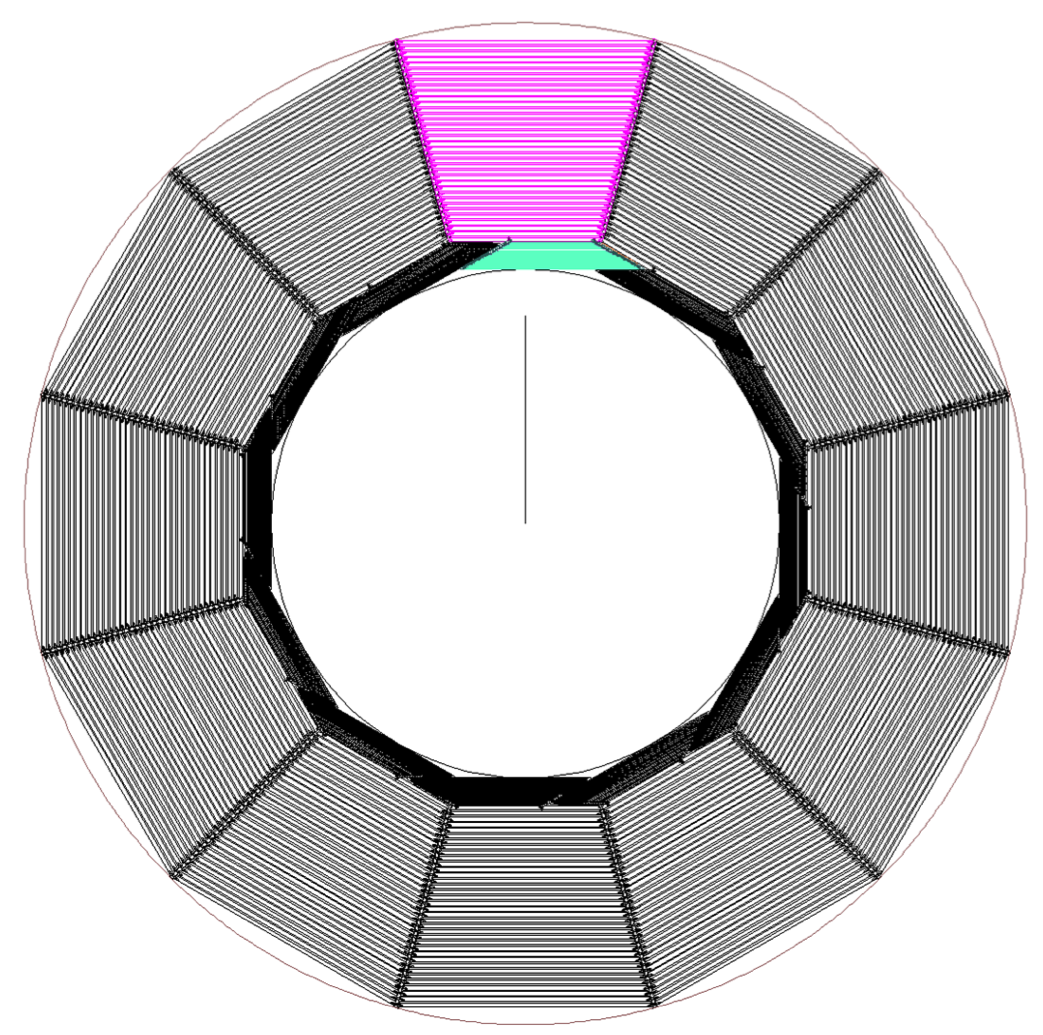
\includegraphics[width=\linewidth]{Calorimeter/SiliconTungstenSiD/cross_section}
		\caption{Outer HCAl and inner ECal barrel}
		\label{fig:Calorimeter:SiDECAL:crosssection}
	\end{minipage}\hfill
	\begin{minipage}[b]{.49\textwidth}
		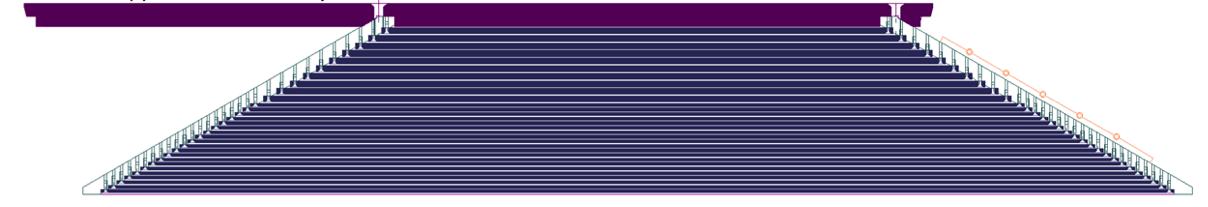
\includegraphics[width=\linewidth]{Calorimeter/SiliconTungstenSiD/ecalModule}
		\caption{ECal module}
		\label{fig:Calorimeter:SiDECAL:ecalModule}
	\end{minipage}
\end{figure}
\begin{figure}
	\begin{minipage}[b]{.29\textwidth}
		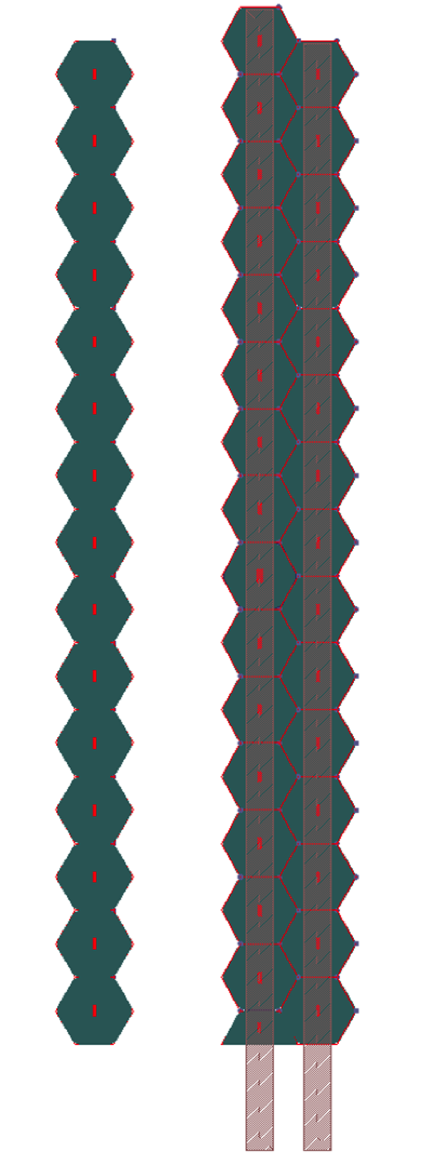
\includegraphics[width=\linewidth]{Calorimeter/SiliconTungstenSiD/hexagon}
		\caption{Hexagonal silicon detectors with flexible circuit interconnects}
		\label{fig:Calorimeter:SiDECAL:hexagon}
	\end{minipage}\hfill
	\begin{minipage}[b]{.65\textwidth}
		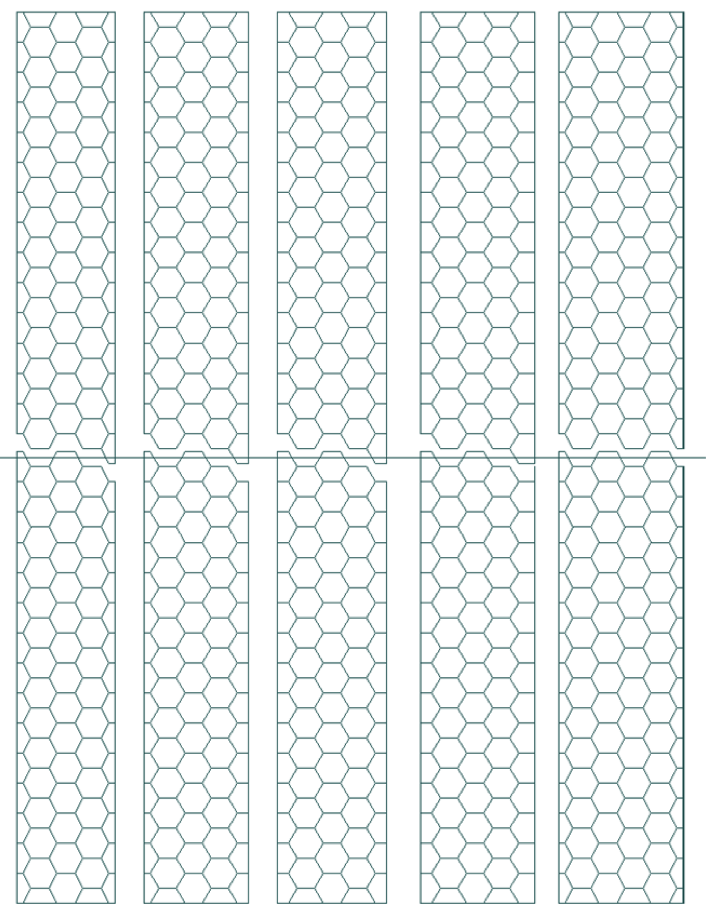
\includegraphics[width=\linewidth]{Calorimeter/SiliconTungstenSiD/siliconLayout}
		\caption{Silicon layout for five outer layers}
		\label{fig:Calorimeter:SiDECAL:siliconLayout}
	\end{minipage}
\end{figure}
\begin{figure}
	\begin{minipage}[b]{.49\textwidth}
		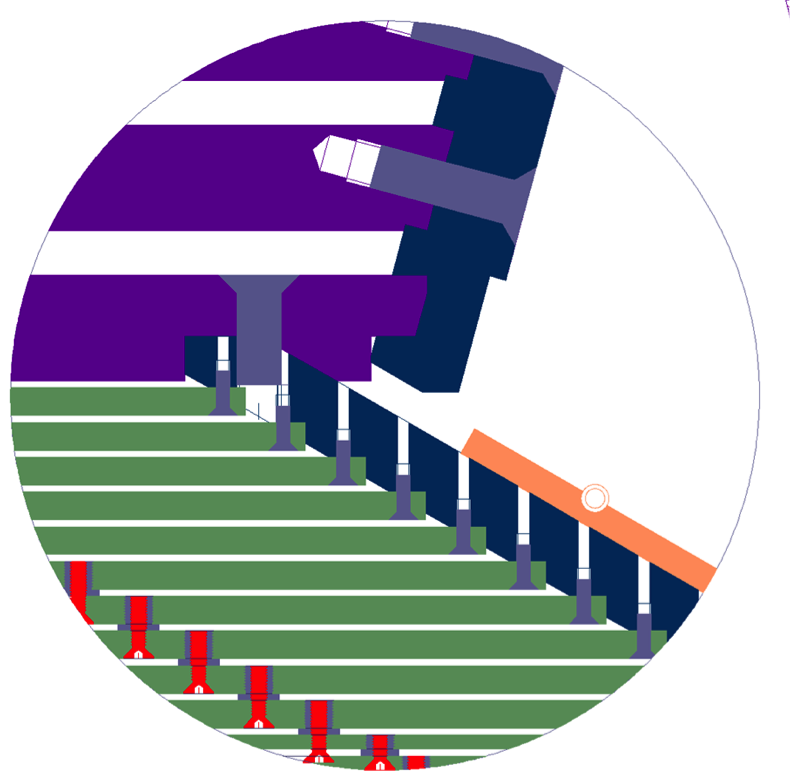
\includegraphics[width=\linewidth]{Calorimeter/SiliconTungstenSiD/edgeFasteners}
		\caption{Edge and field fasteners}
		\label{fig:Calorimeter:SiDECAL:edgeFasteners}
	\end{minipage}\hfill
	\begin{minipage}[b]{.49\textwidth}
		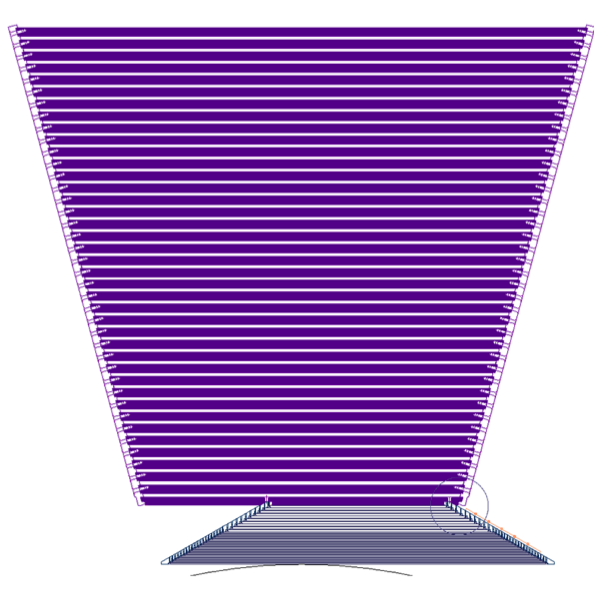
\includegraphics[width=\linewidth]{Calorimeter/SiliconTungstenSiD/ecalMounting}
		\caption{ECal to HCal mounting}
		\label{fig:Calorimeter:SiDECAL:ecalMounting}
	\end{minipage}
\end{figure}
\begin{figure}
	\begin{minipage}[b]{.49\textwidth}
		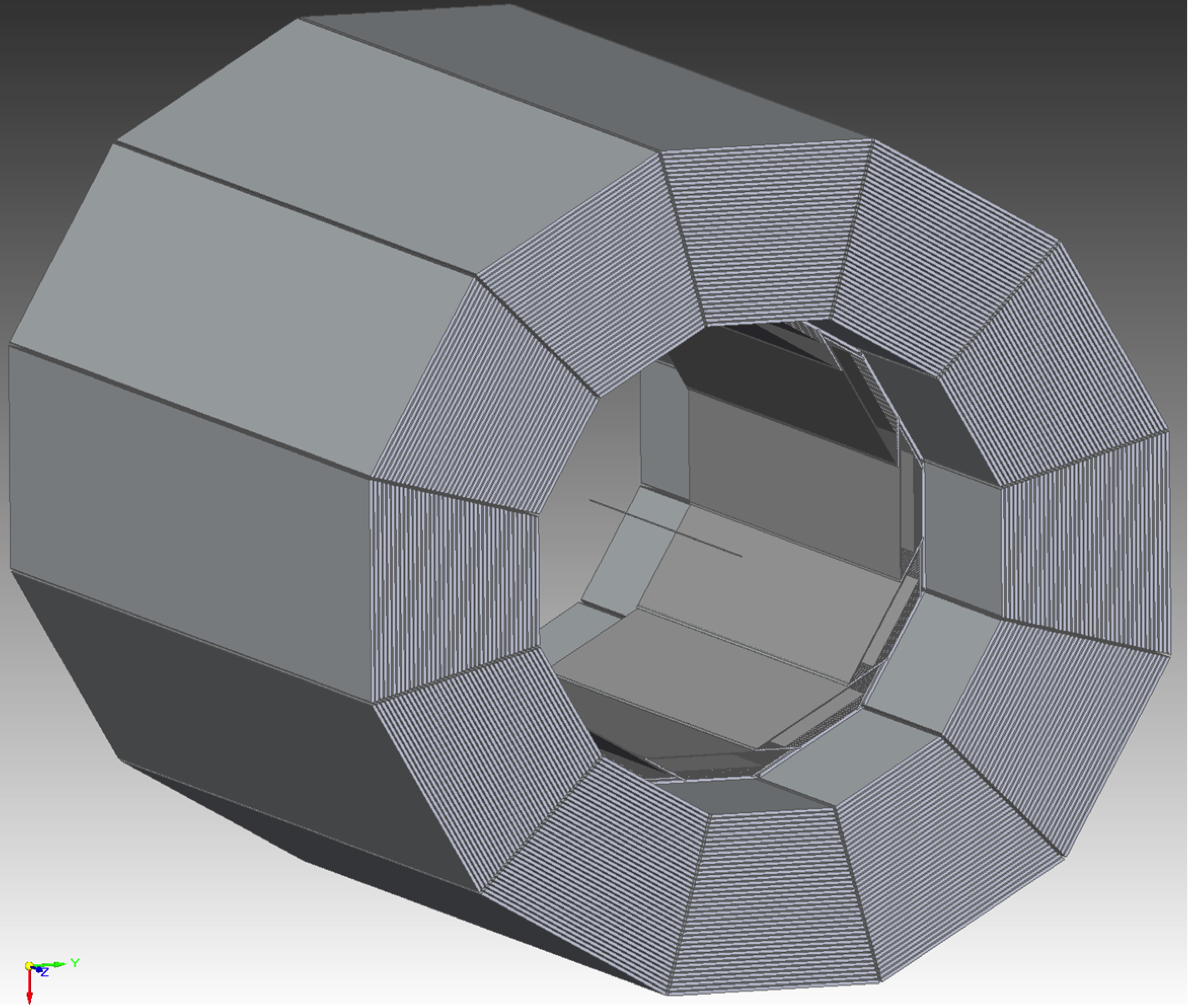
\includegraphics[width=\linewidth]{Calorimeter/SiliconTungstenSiD/HCalECal}
		\caption{HCal with integral ECal detector}
		\label{fig:Calorimeter:SiDECAL:HCalECal}
	\end{minipage}\hfill
	\begin{minipage}[b]{.49\textwidth}
		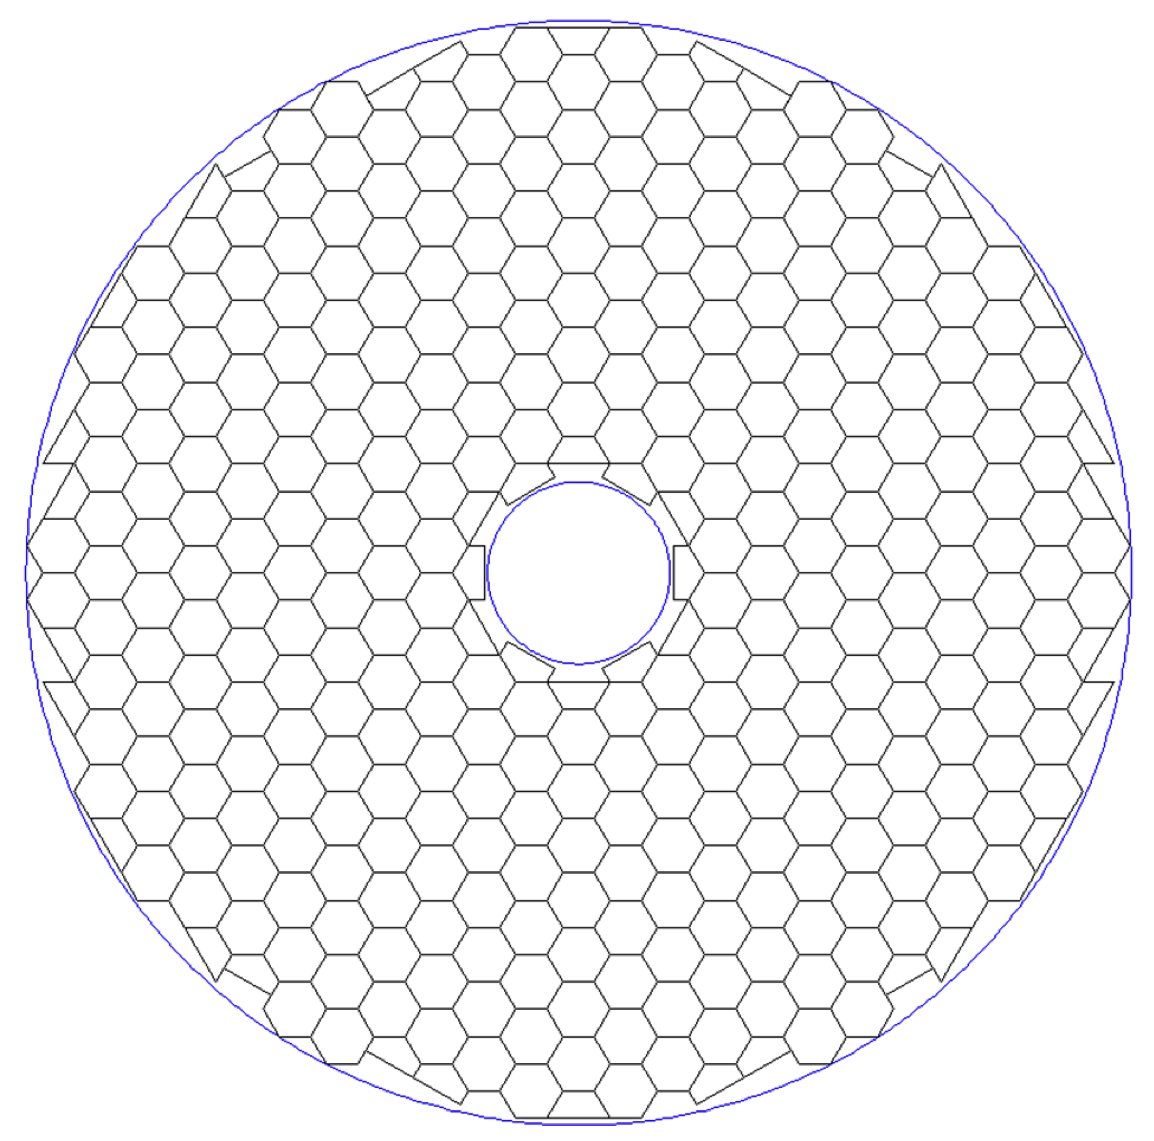
\includegraphics[width=\linewidth]{Calorimeter/SiliconTungstenSiD/endcapLayout}
		\caption{Endcap detector layout}
		\label{fig:Calorimeter:SiDECAL:endcapLayout}
	\end{minipage}
\end{figure}

This note describes the theory of the mechanical aspects of the E-Cal system for
SiD. The E-Cal barrel consists of stacks of tungsten heavy metal plates which
are arranged in modules surrounding the beamline. Full cylindrical coverage of
the baseline design is attained with twelve modules (see Figure~\ref{fig:Calorimeter:SiDECAL:crosssection}) occupying a
radial envelope from \SI{1265}{mm} to \SI{1409}{mm}. The total barrel length is \SI{3.53}{m}. Each
module uses 20 inner plates which are \SI{2.5}{mm} thick followed by ten \SI{5}{mm} thick
plates. Gaps between adjacent plates are \SI{1.25}{mm} and house the silicon detectors
with their associated cables (see Figure~\ref{fig:Calorimeter:SiDECAL:ecalModule}). These hexagonal silicon detectors
are electrically connected to each other with thin, flexible circuits which are
read out on both ends of a module (see Figure~\ref{fig:Calorimeter:SiDECAL:hexagon}). Panels of detectors increase
in width as they get closer to the beamline. To minimize silicon waste and to
maximize coverage, fractions of hexagons complete the panel edges (see Figure~\ref{fig:Calorimeter:SiDECAL:siliconLayout}). By cutting the silicon in strategic locations, only a few different silicon
shapes may be needed to achieve the 31 different panel widths. The tungsten
plates are connected together on their longitudinal edges as well as in the
field of detectors. Space for fasteners in the field is achieved by chamfering
the corners of the hexagonal detectors. The field fasteners hold the plates
together, provide a uniform \SI{1.25}{mm} standoff height, and assist with inter-plate
shear. The fasteners near the edges of the plates close the module profile and
lend torsional rigidity to the structure. An FEA simulation of the proposed
configuration should be done to properly size the fasteners (see Figure~\ref{fig:Calorimeter:SiDECAL:edgeFasteners}).The
modules, which weigh about 5 tons each, are mounted to stainless plates which
are used as the first layer of the next detector system (H-Cal). This first
H-Cal plate is unique in that its two longitudinal edges form a guide system to
locate the E-Cal to the H-Cal system. The H-Cal modules are first bolted
together to form the H-Cal barrel. Interleaving structural side battens maintain
spacing for the H-Cal plates and extend inward to the E-Cal support plates. The
inner ends of these battens act in concert as the female portion of the E-Cal
guide system. The E-Cal modules are slid into place in the inner H-Cal bore.
Extension plates complete the inner H-Cal first layer, since the E-Cal barrel is
shorter. H-Cal detector panels are installed after this structure is complete
(see Figure~\ref{fig:Calorimeter:SiDECAL:HCalECal}). Only simple detector layouts have been done for the E-Cal
endcaps so far. These layouts show that using full and partial hexagons could
yield fairly good coverage with only a few shapes. (see Figure~\ref{fig:Calorimeter:SiDECAL:endcapLayout}).

% \subsection{Participating Institutes}
% SLAC National Accelerator laboratory
% University of California, Davis
% University of California, Santa Cruz
% University of Oregon
% University of New Mexico

\subsection{Introduction}
KPiX is a 1,024 channel ``System on a Chip'' intended for bump bonding to large area Si sensors, enabling low multiple scattering Si strip tracking and high density Particle Flow calorimetry for SiD at the International Linear Collider (ILC).

Each channel consists of a dynamically switchable gain charge amplifier; shaping; threshold discrimination; and 4 sample and hold capacitors and 4 timing registers. The chip permits 4 separate measurements of amplitude and time of threshold crossing during each train, and amplitude digitization and readout during the intertrain period. The dynamic range is from sub minimum ionizing particle (mip) (\SI{320}{\micro\meter} silicon) to more than 2,000 mip. KPiX also has a calibration system for each channel, servos for leakage compensation, ``DC'' reset for asynchronous operation for testing with cosmic rays, and polarity inversion for use with GEMs and similar detectors. The noise floor is about \SI{0.15}{fC} ($\approx 1,000$ electrons), and the maximum signal is \SI{10}{pC} (utilizing the dynamic range switching). The full dynamic range corresponds to 17 bits.

\subsection{Recent Milestones}
ILC related R\&D in the US is largely unfunded and small efforts are being kept alive on the margins. The KPiX R\&D is such an example of necessary work for SiD that is marginally alive.
At this time, KPiX is seen as the baseline readout system for the tracker and electromagnetic calorimeter .  A stack of 13 EMCal sensors with bump bonded KPiX was assembled for a beam test at SLAC in the summer of 2013. That test discovered that two kinds of crosstalk are significant:
\begin{itemize}
	\item In-time crosstalk occurs due to parasitic coupling of traces on metal 2 of the sensor to other pixels. The level of crosstalk increases with the size of the signal, and decreases with increased speed of the front end charge amplifier (meaning increased current and power dissipation).  A new sensor design is being developed that uses metal 1 to shield the traces of metal 2, and these ideas will be tested in the next sensor prototype.
	\item Out-of-time cross talk occurs when many pixels are hit and reset simultaneously. The resets collectively cause other pixels to trigger, and a cascade builds up. This uses up all the KPiX buffers. The root cause of the problem appears to be some internal logic within KPiX that is not current limited, and will require design modification.
\end{itemize}
A more general issue is that both the EMCal and tracker sensors from Hamamatsu were ordered with Al pads, as it was believed that plating (by the zincate process) a stack of metals culminating with Au would be straightforward. This turns out to be wrong. After many attempts at University of California Davis (UCD) and local industry, IZM  has Ar ion etched the pad surfaces and sputtered a base layer, permitting the buildup of a stack that ended with Au, and permitting the attachment with solder bumps that had been placed during KPiX manufacture by TSMC. Testing of these sensors revealed $\approx 10\%$ pixel to pixel shorts and some opens of signal traces, that are suspected to be damage caused by the Ar ion etch. A new round of sensors has been ordered with the Metal 1 layer used to shield the Metal 2 traces from the diodes that they cross on the way to the KPiX bump pads, and with the Au pads being built by Hamamatsu.

An additional issue is that the Tracker sensor was planned to be wire bonded to its (very thin) cable. The sensor oxide layer is not strong enough to allow wire bonding without damage, and so must be solder bumped. The pad pitch is small, and solder bumping the cable will be challenging. The trouble with the wire bonding to the sensor was unexpected. Recent attempts with both bump bonding a cable and utilizing electrically conductive epoxy have failed. The best explanation is that the \SI{150}{\degreeCelsius} thermal cycles associated with these attachments increased the stress on the KPiX bonds and caused the sensor pads to separate from the sensor. It is belived that something went wrong with the Hamamatsu process on both types of sensors, and is related to the wire bonding problem.

Another concern is that the current design of KPiX has deadtime after a pixel has accepted a trigger. Only the triggered pixel is affected; all the other pixels are available for signals. This deadtime is different from the usual notion of data acquisition deadtime where the entire detector is unavailable, but the correction to the luminosity integral is easy. Finally, the buffer requirement (4 in the current version of KPiX) is being re-evaluated in SiD simulations. A possible new architecture for KPiX is in early stages of evaluation. Another approach is the development of Monolithic Active Pixel (MAP) sensors for both SiD sensors using thinned HVCMOS. The sensors would be approximately the same size as the current sensors. The tracker would have $40 \times \SI{500}{\micro\meter}$ pixels, and would only need one buffer. A prototype to evaluate the pixel performance is being designed now. The EMCal sensor will have $1 \times \SI{1}{mm}$ pixels which should limit the required dynamic range and eliminate range switching, but would still need 16 buffers.

A small mechanical engineering effort has started to study the structure of the EMCal. The Sid EMCal has emphasized thin gaps between the tungsten layers to minimize the Moliere radius, and this implies that the structure is connected by columns at the vertices of the sensors. This work has been carried out to the level of a pre-conceptual design.

\subsection{Engineering Challenges}
\subsection{Future Plans}
Assuming positive developments with Japan are announced soon, we expect the financial support to improve. It should be noted that an important effect of the withdrawal of support is that most of the US collaborators have been forced to move to other work.
\begin{itemize}
	\item EMCal Sensors: A second round of prototypes will be designed and ordered with rectangular layout; shielded traces, and Au pads.
	\item Tracker Sensors: The current prototypes will be evaluated, and if appropriate tested in a beam.
	\item KPiX: A new architecture with little (or no) deadtime will be evaluated. A decision will be made to develop this new architecture or incrementally improve the existing design.
	\item The EMCal mechanical structure will be pushed towards a conceptual design.
\end{itemize}

%from arXiv:1212.5127v2
\section{DECAL}
Most recent update: 2014-08-25 \\
Contact person: Jan Strube (email: jan.strube@pnnl.gov)

\subsection{Introduction}
The studies of a digital ECAL (DECAL) in the UK are currently dormant. In December 2008, the STFC Executive recommended sufficient funding
to allow the SPiDER Collaboration to construct a full physics prototype DECAL, as outlined
in~\cite{Adloff:2010aa}. By December 2009, the funding for SPiDER had still not been issued and STFC
informed the Collaboration that they would not do so.

The UK groups in SPiDER have demonstrated that the INMAPS technology developed
specifically for the DECAL application is viable in terms of basic pixel efficiency. INMAPS is
implemented as a \SI{0.18}{\micro\meter} CMOS process in which a deep P-well implant stops signal charge
from being absorbed in N-well circuits, and therefore allows the use of both NMOS and
PMOS within the pixel, as well as (optionally) high resistivity silicon in the thin epitaxial
layer to reduce the charge collection time.

\subsection{Test Beams in 2010}
Following a successful test beam run at CERN in September 2009 using 120 GeV pions, two
further data taking runs have been carried out. The first of these was at DESY in March
2010, for which the primary goal was to quantify the peak electromagnetic shower density
observed downstream of specific absorber materials. A secondary goal was to make further
pixel efficiency measurements. Data were recorded with the 1-5 GeV electron beam, using a
configuration in which four TPAC 1.2 sensors were aligned precisely along the beam direction
using the same custom-built mechanical frame as at CERN. Absorber material (W, Fe, Cu)
was placed downstream of these, followed immediately by a further pair of TPAC sensors, to
study the shower density.

To complement the DESY run, similar, additional data was recorded at CERN in September 2010, using the EUDET telescope alone as it has finer pitch than the TPAC sensor, with positrons between 10 and 100 GeV. The same slabs as those at DESY were used together with
new slabs due to the higher energies available at CERN. Initial results of shower multiplicities
are presented in~\cite{Price:2012vta}.

\subsection{Pixel efficiency results}
The studies of pixel efficiency from CERN 2009 testbeam and DESY were performed using a
set of six TPAC 1.2 sensors aligned along the beam direction, in which the outer four sensors
served as a beam telescope, while the two innermost sensors were considered as the devices
under test. The trajectory of the beam particle was projected onto the plane of both of these
sensors, and each pixel of the test sensors was examined for the presence of hits as a function
of the distance from the projected track. The MIP hit efficiency was determined by fitting
the distribution of hit probability to a flat top function, convoluted with a Gaussian of the
appropriate resolution to allow for finite tracking performance. This efficiency, folded for all
pixels together, is illustrated in Figure~\ref{fig:Calorimeter:DECAL:MIPS}

\begin{figure}
    \includegraphics[width=.49\textwidth]{Calorimeter/DECAL/MIPEfficiency}
    \includegraphics[width=.49\textwidth]{Calorimeter/DECAL/MIPResponse}
    \caption{(left) Distribution of the probability of a pixel registering a hit in response to a MIP, as a function of distance to the projected track, and (right) MIP efficiency as a function of the sensor digital threshold, for all four sensor variants studied.}
    \label{fig:Calorimeter:DECAL:MIPS}
\end{figure}

The MIP efficiency was determined per pixel for both the DESY and CERN data, and for each of the four pixel variants tested. The variants (and corresponding marker color in Figure~\ref{fig:Calorimeter:DECAL:MIPS}) are:

\begin{enumerate}
\item (red) in \SI{12}{\micro\meter} standard (non-INMAPS) CMOS;
\item (black) \SI{12}{\micro\meter} deep P-well CMOS;
\item (green) deep P-well within a \SI{12}{\micro\meter} high resistivity epitaxial layer;
\item (blue) deep P-well within an \SI{18}{\micro\meter} high resistivity epitaxial layer.
\end{enumerate}

The results~\cite{Dauncey:2010zz} are summarized in Figure~\ref{fig:Calorimeter:DECAL:MIPS}, for a range of the sensor digital thresholds representative of the signal levels expected in DECAL pixels due to charge spreading. (A typical MIP signal in a \SI{12}{\micro\meter} epitaxial layer of silicon is 1200 electrons and a single pixel absorbs at most 50\% of this due to charge spreading.)

From the results shown in the figure, it is observed that the standard, non-INMAPS sensors have markedly low efficiencies, which is attributed to signal charge being absorbed by in-pixel PMOS transistors. In contrast, the use of the deep P-well reduces the absorption of signal charge by N-wells in the circuitry, improving very substantially the pixel efficiency by a factor of $\approx 5$. The addition of the high resistivity epitaxial layer further improves the pixel efficiency to $\approx 100\%$.

\subsection{Future plans}
It is no longer an option to plan for a physics prototype DECAL and the short-term future of the DECAL project is extremely uncertain at present. A program of radiation hardness has been conducted on 2011 and the results are summarized in~\cite{Price:2012vta,Price:2013js}. This is in part to understand how the TPAC sensor would satisfy the requirements of ALICE ITS and SuperB . The studies which have been carried out so far are in the process of being finalized, and a series of papers, e.g.~\cite{Ballin:2011jq}, are in preparation to document what has been achieved. The technology development has been taken over by the Arachnid collaboration who are testing the CHERWELL chip (designed and manufactured by the SPiDeR collaboration but never used due to money constraints) to evaluate the performance for ALICE and SuperB.

\section{Analog HCAL}
Most recent update: 2019-12-03\\
Contact person: Felix Sefkow (email: felix.sefkow@desy.de)
\subsection{Introduction}
With the advent of silicon photo-multipliers (SiPMs), the scintillator tile technology became a candidate for highly granular particle flow calorimetry. With analog read-out, energy and spatial resolution can be optimized independently. The particle flow performance is well understood; all published studies using PandoraPFA are based on this technology.

The CALICE AHCAL was the first large LC hadron calorimeter prototype to be exposed to test beams. Analysis is nearly complete and mostly published; the results validate the technology and the simulations.

The development of engineering solutions for a realistic detector is well advanced. The integration of read-out electronics and calibration system into the detector layers has been achieved, and an integrated stack, corresponding to a phi-sector of a barrel calorimeter, has been constructed and exposed to beam tests. In parallel, as drastically improved photo-sensors have become available from industry, the design of the basic read-out cell -- the tile with SiPM -- has been optimized with regard to mass production procedures.

\subsection{Recent Milestones; past and present R\&D}
\subsubsection{Test beam data analysis}
The following results using data taken with the first AHCAL ``physics'' prototype in 2006 -- 2011 at CERN and Fermilab have been published in peer-reviewed journals:
\begin{enumerate}
\item Detector construction, noise and aging studies~\cite{1748-0221-5-05-P05004}
\item Electromagnetic linearity and resolution~\cite{1748-0221-6-04-P04003}
\item Studies using a scintillator SiPM based tail catcher~\cite{1748-0221-7-04-P04015}
\item Geant 4 validation with pion showers~\cite{1748-0221-8-07-P07005}
\item Geant 4 validation with tungsten absorber (low energy)~\cite{1748-0221-9-01-P01004}
\item Imaging capabilities, track segments~\cite{1748-0221-8-09-P09001}
\item Time structure of showers in Fe and W~\cite{1748-0221-9-07-P07022}
\item Geant 4 validation with protons~\cite{1748-0221-10-04-P04014}
\item Geant 4 validation with tungsten absorber (high energy)~\cite{Blaising:2015nla}
\item Hadron shower decomposition~\cite{Price:2016sce}
\end{enumerate}

We consider all of them as critical for validating a given HCAL technology. Papers~\cite{1748-0221-8-07-P07005, 1748-0221-9-01-P01004, 1748-0221-8-09-P09001, 1748-0221-9-07-P07022, 1748-0221-10-04-P04014, Blaising:2015nla, Price:2016sce} appeared after the ILC TDR was handed over.

\emph{Preliminary} results have been made public in the form of \emph{CALICE Analysis Notes} after thorough internal reviewing on the following topics:
\begin{enumerate}
\item Leakage estimation using shower topology~\cite{Marchesini:CAN029}
\item Analogue, Digital and Semi-Digital Energy Reconstruction~\cite{Calice:CAN049}
\end{enumerate}
The second of these notes appeared in the time since the release of the ILC TDR.
The following notes have progressed to the level of publications.
\begin{enumerate}
	\item Pion Response and Resolution in a Combined Scintillator Calorimeter System~\cite{Repond:2018flg}
	\item Energy Reconstruction of Hadrons in a Highly Granular Si-W ECAL and Plastic Scintillator HCAL Calorimeter System~\cite{Israeli:2018byq}
\end{enumerate}
	
With these papers the analysis of the first-generation test beam data is considered complete.

The CALICE test beam results are nowadays the primary source of validation for hadron shower simulation, according to Geant 4 representatives, and extremely valuable for other HEP experiments, e.g. at the LHC, as well.

With the first round of data taking with the second-generation full-scale prototype~\cite{Sefkow:2018rhp} accomplished in May and June 2018, several $10^7$ beam events are available to new analyses, in particular studies including the time domain of hadronic shower evolution.

We finally note that test beam analysis plays an important role in training our students. Roughly speaking, each paper or note corresponds to one or several PhD theses. It is a distributed effort; the corresponding editors of the papers are from about 10 different groups.

\subsubsection{Optimization of the scintillator SiPM read-out cell}
\label{sec:OptimizationSiPMRO}

\begin{figure}
	\centering
	\includegraphics[width=.5\linewidth]{Calorimeter/AHCAL/DarkCount}
	\caption{Dark count rate of recent SiPMs, MPPC devices by Hamamatsu, without (standard) and with (new) inter-pixel cross talk suppression. ({\it Courtesy MPI for Physics, Munich})}
	\label{fig:Calorimeter:AHCAL:DarkCount}
\end{figure}

As a consequence of the wide success of SiPM applications in other fields, e.g. in medical imaging, the development of improved sensors is dynamically pursued in industry, and several groups are in close contact with leading producers. Progress has been made in terms of dark rate (see Figure~\ref{fig:Calorimeter:AHCAL:DarkCount}), noise above MIP threshold and dynamic range. For comparison, typical SiPMs in the first generation prototype had a dark rate of about 2 MHz and a cross talk probability of about 25\%. In addition, the samples are much more homogeneous than at the time of the first prototype, which results in a strong simplification of commissioning and calibration procedures.

In the time since the TDR, scintillator tile SiPM units without wave-length shifting fiber have been developed for the integration of SiPMs into the electronics read-out board, as originally proposed in~\cite{Blazey:2009zz}. Following geometry optimization~\cite{2010NIMPA.620..196S,Liu:2015cpe}, the tiles are injection-moulded and wrapped individually in reflector foil. They have been integrated into a partially instrumented absorber stack and tested with beams at DESY and CERN in 2014 -- 2015.

Industrialization of the SiPM and tile design has been addressed, and assembly procedures with industrial facilities such as automatic pick-and-place machines have been established. 

\begin{figure}
	\centering
	\includegraphics[width=0.5\textwidth]{Calorimeter/AHCAL/SurfaceMountedTiles}
	\caption{AHCAL read-out board with surface-mounted SiPMs and tiles. ({\it Courtesy University of Mainz})}
	\label{fig:Calorimeter:AHCAL:HBU}
\end{figure}

The studies converged on the current design, with photo-sensors integrated in the read-out electronics board, which results in further simplifications, i.e., cost and time savings, but poses higher performance requirements to the SiPM, which can met with the latest generation of SiPMs. This design is shown in Figure~\ref{fig:Calorimeter:AHCAL:HBU}. A quality assurance and integration chain has been worked out that is also scalable to the mass production as required for a LC detector.

\subsubsection{Electronics and active layer integration}

The design of the active layers with integrated read-out ASICs and calibration system~\cite{6829522} had been basically validated in beam tests of a single HCAL layer consisting of four base units (HBUs) at CERN in 2012 and reported in the TDR. An HBU reads $12 \times 12$ tiles with 4 ASICs. The present ASIC~\cite{1748-0221-6-01-C01098} belongs to the 2nd generation ROC family used also in ECAL and SDHCAL. An HCAL layer carries interfaces for DAQ, calibration and power supply, which already have a compact design fulfilling space constraints at an ILC detector.

The main functional difference between the integrated electronics and that of the physics prototype is the self-triggered operation and on-detector zero-suppression, which implies much higher demands on controlling the noise behavior and ensuring a stable detector response. It is thus mandatory to re-establish the calorimeter performance with a full-scale beam test, including the operation with fast power cycling.

Further R\&D in the next years has to be done on the ASIC. The 3rd generation ASIC will have a more robust slow control architecture and possibly channel-wise buffer management, which improves rate capabilities. In parallel, an alternative design of the analog part, which can handle a larger range of sensor, has been finished and needs to be integrated into the read-out board and digital data handling.

\subsubsection{System Integration}

\begin{figure}
	\centering
	\includegraphics[width=.5\textwidth]{Calorimeter/AHCAL/AHCAL_Stack}
	\caption{Partially instrumented AHCAL stack with integrated read-out electronics and data concentrator for two complete modules.({\it Courtesy DESY})}
	\label{fig:Calorimeter:AHCAL:Stack}
\end{figure}

In parallel to the integration of layers, that of entire stacks or modules has been pursued. Since the TDR release, efforts concentrated on developing a multi-layer DAQ capable of reading larger systems~\cite{Kvasnicka:2017bpx}. This was ready for beam tests at CERN in fall 2014. It involves integration of a dedicated module data concentrator (see Figure~\ref{fig:Calorimeter:AHCAL:Stack}), which collects signals from all layers of two phi-sectors for sending them to the off-detector data receiver. The HCAL DAQ has been integrated into the higher level system EUDAQ2 for the purpose of combined beam tests, for example with a tracking device for uniformity studies, or with an ECAL for inter-calibration and combined performance. The same is true for slow control data.

A power supply system based on commercially available modules has been set up; an alternative custom system with optimized channel density per module is being developed.

It has been demonstrated that temperature-induced variations of the SiPM gain can be compensated by adjusting the bias voltage. The approach stabilizes the detector response and trigger efficiency and thus simplifies operations significantly. Automatic procedures based on this principle have been developed and implemented at system level.

\subsubsection{Infrastructure for production, quality assurance and characterisation}

The AHCAL is probably the sub-detector with the largest number of individual components. While the number of electronics boards, layers and interfaces is similar to other ECAL or HCAL options, the large quantity of tiles and SiPMs deserves special attention. This affects production and also quality assurance.

While it would be premature to build up full production infrastructure, already for the second generation full-scale prototype with its 22000 channels, conceptual solutions had to be developed~\cite{Munwes:2634923} and exercised using demonstrators, which could be seen as prototypes of future installations.

Spot-samples of all 40 SiPM lots, and each one of the 640 ASICs, had undergone semi-automatic testing procedures before soldering the HBUs. Without any further surface treatment, injection-moulded scintillator tiles have been wrapped in laser-cut reflective foil by a robotic procedure and mounted on the HBUs using a pick-and-place machine, after glue dispensing with a screen printer. Cosmic test stands were used to assure the quality of the assembly, to monitor the uniformity of the light yield over the production period and within HBUs, and to obtain an initial MIP calibration.

\subsubsection{Prototype integration and test beam operation}
 The HBUs have been integrated into cassettes with interfaces for DAQ, LED pulsing and power distribution, which provide active compensation of temperature variations by automatic adjustments of the common bias voltage of the photon sensors in each layer. Figure~\ref{fig:AHCAL:ActiveLayer} shows the top side of one active layer, with the scintillator tiles visible. All layers have been calibrated in the DESY test beam, and all channels except eight (0.4‰) are working.

 \begin{figure}
	\centering
	\includegraphics[width=.5\linewidth]{Calorimeter/AHCAL/AHCalActiveLayer}
	\caption{AHCAL active layer side with wrapped tiles on 4 HBUs, with interfaces for DAQ, LEDs and power. ({\it Courtesy DESY})}
	\label{fig:AHCAL:ActiveLayer}
 \end{figure}

Finally, the calibrated layers were assembled into the absorber stack and connected to data concentration, power distribution and cooling services. Figure~\ref{fig:AHCAL:FullStack} shows the active layers with connected services inserted in the absorber structure. The full prototype has been commissioned with cosmic muons, exploiting its self-triggering capabilities.

\begin{figure}
	\centering
	\includegraphics[width=.5\linewidth]{Calorimeter/AHCAL/AHCalStack}
	\caption{Fully integrated SiPM-on-tile AHCAL engineering prototype. ({\it Courtesy DESY})}
	\label{fig:AHCAL:FullStack}
\end{figure}

The prototype has been installed in the test beam for data taking at the CERN SPS. In two periods in May and in June 2018, several $10^7$ events with muon tracks as well as electron and pion showers at various energies in the range from 10 GeV up to 100 GeV for electrons and 200 GeV for hadrons have been collected. The data taking rate averaged over the about 5s long spills and was up to 400 events per second. Figure~\ref{fig:AHCAL:EvtDisplay} shows two event displays, a cosmic muon and a high-energy pion shower.

\begin{figure}
	\centering
	\includegraphics[width=.49\linewidth]{Calorimeter/AHCAL/AHCalEvtDisplay1}
	\includegraphics[width=.49\linewidth]{Calorimeter/AHCAL/AHCalEvtDisplay2}
	\caption{AHCAL event displays: cosmic muon and high energy pion ({\it Courtesy DESY})}
	\label{fig:AHCAL:EvtDisplay}
\end{figure}

The rich data sample collected in the two test beam periods in 2018 will be used for shower separation studies based on 5-dimensional reconstruction algorithms exploiting the high spatial, energy and time resolution of this novel detector.

\subsubsection{Mechanics and Cooling}

The absorber structure bears more challenges than for conventional hadronic calorimeters. Due to the much finer longitudinal segmentation and the imperative to minimize the total radius inside the coil, there are many active gaps with tight tolerances. A design has been developed and prototyped, which achieves the required tolerances with a cost-effective roller-leveling process without machining off excess material. Two test structures have been built; one -- used also for the test beam prototype -- covers the full transverse cross section of a barrel module, the other the full lateral extension. The cassettes housing the active elements have the final design and are used in beam tests.

These structures need to be investigated with respect to their robustness against earthquakes. Simulations of the whole ILD structure have been made, and measurements on the test structures exposed to accelerating forces should be done in order to check the simulations. The results of the simulation will be used to optimize the structural design.

A cooling system has been developed. The ASICs integrated in the detector layers are power-pulsed and do not need active cooling, but the interfaces, in particular the power regulators, do. The solution developed for beam tests is already laid out for a leak-less under-pressure based system.

As enough active elements become available for instrumenting several active layers at full size, the thermal simulations should be verified with measurements using the second lateral test structure, too. This will constitute an important step in system integration, as it addresses the issues associated with large layers and in particular power distribution, power cycling and heat dissipation.

\subsection{Summary}
The AHCAL effort has produced a number of significant results in the time since the ILC TDR:
\begin{itemize}
\item Publication of 7 journal papers and 4 preliminary conference results in the form of internally reviewed notes, on Geant 4 validation with pions and protons in steel and tungsten, including new observables like track segments
\item Development, construction and beam test of a second-generation full-size prototype with a new, simplified tile SiPM system with improved sensor performance, using a design and production and QA procedures scalable to a full ILC detector
\end{itemize}

\subsection{Future Plans}

The AHCAL has accomplished the essential step towards a technical design report with a realistic full-scale prototype. Coordinated R\&D is required in the following areas:

\begin{itemize}
\item 2nd generation prototype reconstruction and simulation software
\item Development of timing reconstruction
\item Analysis of 2nd generation test beam data
\end{itemize}

\subsection{Engineering Challenges}

Electronics:
\begin{itemize}
\item establish power-pulsed operation of large layers
\item 3rd generation ASIC of ROC family
\item ASIC for larger range of SiPM gains
\end{itemize}

Absorber structure:
\begin{itemize}
\item Earthquake stability calculations and tests
\item Thermal tests with full-scale instrumented and powered structures
\end{itemize}

There are ample opportunities for new groups to join into any of these fields, depending on the special competences they wish to contribute.

\section{Glass RPC SDHCAL}
Most recent update: 2018-06-07 \\
Contact person: Imad Laktineh (email: laktineh@ipnl.in2p3.fr)
\subsection{Introduction}

Hadronic calorimeter (HCAL) plays an essential role in PFA-based experiments as
those proposed for the ILC. It allows to separate the deposits of charged and
neutral hadrons and to precisely measure the energy of the neutrals. The
contribution of the neutrals to the jet energy, around 10\% on average,
fluctuates in a wide range from event to event, and the accuracy of the
measurement is the dominant contribution to the particle flow resolution for jet
energies up to about \SI{100}{GeV}. For higher energies, the performance is
dominated by confusion, and both topological pattern recognition and energy
information are important for correct track cluster assignment.
High-granularity hadronic calorimeter is thus needed to achieve excellent jet
energy resolution.

HCAL proposed for both projects of ILC (ILD and SiD), are sampling calorimeters
with steel as absorber and scintillator tiles or gaseous devices with embedded
electronics for the active part. The steel was chosen due to its rigidity which
allows to build self-supporting structure without auxiliary supports (dead
regions). Moreover, the moderate ratio of hadronic interaction length
($\lambda_I = \SI{17}{cm}$) to electromagnetic radiation length ($X_0 = \SI{1.8}{cm}$) of
iron, allows a fine longitudinal sampling in terms of $X_0$ with a reasonable
number of layers in $\lambda_I$, thus keeping the detector volume and readout
channel count small. This fine sampling is beneficial both for the measurement
of the sizable electromagnetic energy part in hadronic showers as for the
topological resolution of shower substructure, needed for particle separation.

For the ILD project we propose gaseous detectors for the HCAL active layers: The
Resistive Plate Chamber (RPC). This is motivated by the excellent efficiency
and very good homogeneity the gaseous detectors could provide. Another
important advantage of gaseous detectors is the possibility to have very fine
lateral segmentation. Indeed, in contrast to scintillator tiles, the lateral
segmentation of gaseous devices is determined by the electronics readout used to
read them. Active layer thickness is also of importance for what concerns the
ILC hadronic calorimeter to be placed inside the magnetic field. Highly
efficient gaseous detectors can indeed be built with a thickness of less than
\SI{3}{mm}.

To obtain excellent resolution of hadronic shower energy measurement using a
binary readout, a lateral segmentation of few millimeters is needed. This
however leads to a huge number of electronics hardly affordable for the future
ILC hadronic calorimeters. $1\times \SI{1}{cm^2}$ cells were found to be a good compromise
that still provides very good resolution at moderate energies. However,
simulation studies show that saturation effects are expected to show up at
higher energies ($> \SI{50}{GeV}$). This happens when many particles cross
one cell in the center of the hadronic shower. To reduce these effects, the
choice of multi-threshold electronics (Semi-Digital) readout was envisaged to
improve on the energy resolution by exploiting the particle density in more
appropriate way.

High-granularity calorimeters imply however a huge number of electronics
channels to operate them. This has two important consequences. The first is the
power consumption and the resulting increase of temperature which affects the
behavior of the active layers. The other consequence is the number of service
cables needed to power, read out these channels. These two aspects can
deteriorate the performance of the HCAL and destroy the principle of PFA if
they are not addressed properly.

The R\&D pursued by the SDHCAL-GRPC groups has succeeded to pass almost all the
technical hurdles of the PFA-based HCAL. The SDHCAL-GRPC groups have succeeded
to build the first technological prototype of these new-generation calorimeters
with 48 active layers of GRPC, $\SI{1}{m^2}$ each. The prototype validates the concept
of high-granularity gaseous detector and permits to study the energy resolution
of hadrons one can obtains with such calorimeter.


\subsection{Readout Electronics}

The readout electronics of the two Semi-Digital HCAL (SDHCAL) projects were
developed in common. An ASIC called HARDROC was first developed to read out the
GRPC detectors proposed for the ILD project. To solve the problem of
connections related to the high number of electronics channels, the option of a
detector embedded electronics using the DAISY chain scheme was chosen and
Printed Circuit Board (PCB) were conceived for the readout of large detectors
GRPC.

\subsubsection{Front-end ASIC}

The HARDROC chip (HR) implements a multi-threshold readout which integrates the
functionalities of amplification, shaping, digitization, internal triggering and
local storage of the data. Each of its 64 channels consists of a fast low
impedance current preamplifier with 8-bit variable gain (in the $[0,2]$ range)
followed by 3 fast shapers (\SI{15}{ns} shaping time). A low offset discriminator is
present on each path and the three corresponding thresholds establish the
multi-level readout. The thresholds are set using three integrated 10-bit
Digital to Analog Converters (DAC). The outputs of the three discriminators are
then encoded 3-to-2 bit and stored in an internal digital memory latched by a
trigger event.

A trigger is generated when one of the lowest level discriminators is fired but
can also be configured on the other thresholds. A frame consists of the 64
encoded discriminator outputs, plus a 24-bit time-stamp and a chip identifier is
stored after a trigger is received. Noisy channels could be easily masked via
the configuration parameters control. In order to avoid fake triggers produced
by noisy channels, the output of each discriminator can be switched off from the
trigger generator logic via the configuration parameters control (Slow Control
hereafter) commands. The response of all the channels can be calibrated by
injecting an analog signal through an integrated $\SI{2+-0.02}{pF}$ input test
capacitor; this is a useful tool to make the response of the different channels
as uniform as possible~\cite{1748-0221-6-02-P02001}.

The ASIC contains a 127-frame long digital memory. This allows to work in a
triggerless mode and keep all the data accumulated during the bench crossing.
Once the memory is full the acquisition is stopped, the readout is performed
and the ASIC can start acquisition again. The Gray-coded time-stamp is derived
from an external \SI{5}{MHz} clock.

An essential feature of the HR is the possibility to be operated in the
power-pulsing mode (PP) that consists of switching off almost all
power-consumption functionalities in between the bench crossings (BC) of the ILC
electron beams. With the ILC duty cycle of one \SI{1}{ms} of BC every \SI{200}{ms}, this
mode allows a reduction factor of more than 100 of power consumption. Thanks to
this reduction, the temperature increase of the HCAL is moderate and only
simple cooling system is needed to operate it efficiently.

\subsubsection{Active Sensor Units}

To read out the $\SI{1}{m^2}$ detector of the SDHCAL, an electronic board with the
same size is needed. This electronic board is an important piece in the present
design. It hosts both the pick-up pads and the ASICs in addition to the
connections linking the pads to the ASICs and those among the different ASICs.
To ensure good transmission qualities and low cross-talk, 8-layer Printed
Circuit Board (PCB) is designed. Feasibility constraints, make the tasks of
circuit production, components soldering, testing and handling of the
assemblies, exceedingly difficult in the case of a single board of one square
meter. The solution of dividing that circuit into 6 smaller but more
manageable PCB was adopted. Each of these small ASUs hosts 24 chips to read out
$48\times 32$ pads of $\SI{1}{cm^2}$ each. This dressed PCB is dubbed Active Sensor
Unit (ASU). The base pattern connecting 64 pads arranged in a $8\times 8$ matrix
to the ASIC's pins is shown in Figure~\ref{fig:Calorimeter:SDHCAL_GRPC:asicPins}. This is identical to the
one used in the ASUs of the small GRPC chambers described in reference
\cite{1748-0221-6-02-P02001}. The routing of each input signal from its own pad up to chip pin
has been carefully optimized to reduce the cross-talk. All input signals are
laid out in the same analog signal layer witch is sandwiched between two GND
layers. The routing of digital signals was kept well separated from the vias
connecting signals from one layer to another. In the case of the GRPC related
ASU, the HARDROC base pattern is replicated $4\times 6$ times in the $\SI{33.33}{cm}
\times \SI{50}{cm}$ board. 4 \SI{1.6}{mm} diameter holes are present on the four
angles of a PCB to be used for fixation purposes as will be explained later.
The rooting was conceived so two of the ASUs can be associated to form one slab
hosting 48 ASICS. Each slab is then connected to one Detector InterFace board
(DIF). The connection between the DIF and the slab as well as the connection
of the two ASUs is performed thanks to tiny connectors allowing the
different clocks, signals as well as the power to circulate between the two
ASUs. Three slabs are then assembled to form the required electronics board.
To ensure the same electric reference level for the six ASUs, the GND layer of
the six ASUs is connected thanks to a copper gasket on all the common sides.
Similar schemes could be proposed for GRPC detectors with larger size.


\begin{figure}
\centering
\includegraphics[width=.7\columnwidth]{Calorimeter/SDHCAL_GRPC/figures/HR2_base.jpg}
\caption{Pads connection to the ASIC's pins}
\label{fig:Calorimeter:SDHCAL_GRPC:asicPins}
\end{figure}


\subsubsection{Front-end and back-end boards}

The interface between the ASUs and the data acquisition system (DAQ) is realised
by the detector interface board called DIF. The main elements of the DIF is an
FPGA and USB, HDMI and SAMTEC connectors. It manages the control signals
(e.g. clock, busy/ready, external/internal trigger, power-pulsing) and
supply power to the ASICs and also performs the readout of the ASIC memories.
DIFs are read out by other FPGA-based boards called Data Concentrator Cards
(DCC). They can be connected up to 9 DIFs through HDMI links and are controlled
by a synchronous DCC (or SDCC). The SDCC can connects to up to 9 DCCs to which
it distributes the clock and the commands. It is also connected to the computer
network for the user to control the DAQ.

In the case of Micromegas ASUs, a small additional board called inter-DIF is
used between the DIF and ASU to provide the high voltage to the meshes and drift
electrode.


\subsubsection{Acquisition Software}

To exploit the data collected by the SDHCAL detectors an acquisition software
was developed. This software is organized in three parts. The first one allows
to access the hardware devices (DIF, SDCC) through an FTDI chip associated to
each of these devices. It transmits the configurations parameters to ASICs
through these devices and collect the data as well. The second part is the
configuration data base. It gives the possibility to store and retrieve all
parameters needed by the DAQ system. The database itself is hosted on an Oracle
server at CC IN2P3 (Villeurbanne, France). To interface this SQL database with
the DAQ software and to allow users to insert and query data without knowledge
of SQL, a C++ library has been written. A special care was taken to allow to
download the parameters associated to a given parameters of the prototype
(roughly 550000 parameters) in few seconds. The third part concerns the data
collection. Data from different DIFs may be readout at a different times but
will have the same Bench Crossing IDentifier (BCID) for a given trigger. The
logical way to keep synchronicity is to store in a BCID indexed map the buffers
of all read DIFs but it requires to man-age memory allocation, access and
cleaning. This was achieved thanks to the abilities offered by recent Linux
kernels to use file based shared memory. In addition, whenever several
computers are involved in the data taking, as it is the case for the SDHCAL
prototype, a communication framework is needed. The CMS data acquisition XDAQ
framework was chosen. This provides communication tools with both binary and
XML, an XML description of the computer and software architecture, a web-server
implementation of all data acquisition application and a scalable event builder.
A monitoring system was also developed to have a online follow-up of the
acquisition during data collection.

\subsection{GRPC-SDHCAL for ILD}
\subsubsection{Detector Development}

The structure
of GRPC proposed as an active layer of the HCAL proposed for ILD is shown in
Figure~\ref{fig:Calorimeter:SDHCAL_GRPC:chamber}. It is made out of two glass plates of \SI{0.7}{mm} and \SI{1.1}{mm}
thickness. The thinner is used to form the anode while the the thicker forms
the cathode. Ceramic balls of \SI{1.2}{mm} diameter are used as spacers between the
glass plates. The balls are glued on only one of the glass plates. In
addition to those balls, 13 cylindrical fiber-glass buttons of \SI{4}{mm} diameter
are also used. Contrary to the ceramic balls the buttons are glued to both
plates ensuring thus a robust structure.

Special spacers (ceramic balls) were used to maintain uniform gas gap of \SI{1.2}{mm}.
Their number and distribution were optimized to reduce the noise and dead
zones ($0.1 \%$). The distance between the spacers (\SI{10}{cm}) was fixed so that
the deviation of the gap distance between the two plates under the glass weight
and the electric force does not exceed \SI{45}{microns}. The choice of these spacers
rather than fishing lines was intended to reduce the dead zones ($0.1 \%$). It
was also aimed at reducing the noise contribution observed along the fishing
lines in standard GRPC chambers. The gas volume is closed by a \SI{1.2}{mm} thicks
and \SI{3}{mm} wide glass-fiber frame glued on both glass plates. The glue used for
both the frame and the spacers was chosen for its chemical passivity and long
term performance.

The resistive coating on the glass plates which is used to apply the high
voltage and thus to create the electric field in the gas volume was found to
play important role in the pad multiplicity associated to a mip \cite{1748-0221-6-02-P02001}.
To find the best coating for GRPC chambers many products were tested. Finally, a
new product based on two components was chosen. By changing the two components
ration one can obtain the needed surface resistivity. Commercial products like
Licron\texttrademark and Statguard\texttrademark which are used for Electro-Static
Discharge (ESD) applications were tried and few $\SI{1}{m^2}$ chambers were built
using those products and intensively tested. Both products failed to satisfy our
application either for long term stability under the high voltage (Licronusing
those products ) or due to the impossibility to obtain the surface uniformity
needed for our application (Statguardusing those products ). Eventually, two
products were identified, both of which are based on colloids containing
graphite. Both can be applied using the silk screen print method, which ensures
very uniform surface quality. One of these products is a single component paint
with a dry surface resistivity of \SIrange{1}{10}{\mega\ohm\per\square}. The second product
comes as two components which must be mixed by the user. The surface resistivity
may be adjusted over a wide range by changing the mix ratio. Both products
require baking at around \SI{170}{\degreeCelsius} to attain a stable surface resistivity.
One product based on colloids containing graphite was finally selected. The
product can be applied using the silk screen print method, which ensures very
uniform surface quality. In addition, the product is made of two components and
it was found that by changing the mix ratio the surface resistivity may be
adjusted over a wide range.

The measured surface resistivity at various points over a $\SI{1}{m^2}$ glass coated
with the previous paint showed a mean value of $\SI{1.2}{\mega\ohm\per\square}$ and a
ratio of the maximum to minimum values of less than 2. A study was also made of
the repeatability of the surface resistivity between different mix batches. It
was found that surface resistivity in the range $\SIrange{0.5}{2}{\mega\ohm\per\square}$ could be
reliably reproduced. For $\SI{1}{m^2}$ GRPCs the painting is applied on the whole
glass plate except for \SI{3}{mm} from the edges. This distance, corresponding to the
frame width, was optimized so the dead zone of the detector is reduced while
external sparks due to the presence of the metallic cassette in the vicinity is
completely eliminated.

Another important aspect of this development concerns the gas circulation within
the GRPC taking into account that for ILD SDHCAL gas outlets should all be on
one side. A genuine system was proposed. It is based on channeling the gas
along one side of the chamber and releasing it into the main gas volume at
regular intervals. A similar system is used to collect the gas on the opposite
side. A finite element model has been established to check the gas
distribution~\cite{Bedjidian2010120}. The simulation confirms that the gas speed is
reasonably uniform over most of the chamber area.


In order to improve on the gas distribution in large chambers taking into
account the requirement that both gas outlets should be on the same side of the
detector to satisfy all possible mechanical structures proposed for ILD
hadronic calorimeter, new schemes were studied. The one we finally adopted
allows us to improve the gas distribution by channeling the gas along one side
of the chamber and releasing it into the main gas volume at regular intervals
thanks to \SI{1.2}{mm} diameter PEEK\texttrademark tubes fixed \SI{2}{cm} from the
chamber side. A similar system is used to collect the gas at the other side of
the chamber. A finite element model has been established to check the gas
distribution~\cite{Bedjidian2010120}. The simulation confirms that the gas speed is
reasonably uniform over most of the chamber area. as can be seen in
Figure~\ref{fig:Calorimeter:SDHCAL_GRPC:gas_distribution}.

The GRPC and its associated electronics are housed in a special cassette which
protects the chamber and ensures that the readout board is in intimate contact
with the anode glass. The cassette is a thin box consisting of \SI{2.5}{mm} thick
stainless steel plates separated by \SI{6}{mm} wide stainless steel spacers. Its
plates are also a part of the absorber.

The electronics board is assembled thanks to a polycarbonate spacer which is
also used to fill the gaps between the readout chips and to improve the overall
rigidity of the detector. The electronics board is fixed on the small plate of
the cassette. Thanks to tiny screws and the new set is fixed on the other plate
which hosts the detector and the spacers. The whole width of the cassette is \SI{11}{mm}
with only 6 of them corresponding to the sensitive medium including the GRPC
detector and the readout electronics.


\begin{figure}
\centering
\includegraphics[width=0.70\textwidth]{Calorimeter/SDHCAL_GRPC/figures/chamber}
\caption{Cross-section through a $\SI{1}{m^2}$ chamber}
\label{fig:Calorimeter:SDHCAL_GRPC:chamber}
\end{figure}


\begin{figure}
\centering
\includegraphics[width=.9\textwidth]{Calorimeter/SDHCAL_GRPC/figures/gas.png}
\caption{Left: Gas speed profile in the range \SIrange{0}{1}{mm/s}; Right: Least mean age profile in the range \SIrange{0}{10}{s}}
\label{fig:Calorimeter:SDHCAL_GRPC:gas_distribution}
\end{figure}

\subsection{Prototype}

A technological prototype corresponding to the SDHCAL option proposed in the ILC
LOI was built. 48 cassettes as the one described above were built. They
fulfilled a stringent quality control. It is worth mentioning that 10500 HR
ASICs were produced and tested using a dedicated robot for this purpose. The
yield was found to be higher than 92\%. The ASICs were then fixed on the PCBs
to make a $\SI{1}{m^2}$ and itself fixed on the cassette cover once successfully
tested.

The cassettes were inserted in a self-supporting mechanical structure that was
conceived and built in collaboration with the Spanish group of CIEMAT. The
structure is made of Stainless Steel plates of \SI{1.5}{cm} each. The plates were
machined to have an excellent flatness and well controlled thickness. The
flatness of the plates was measured using a laser-based interferometer system.
It was found that the flatness of the plates are less than 500 microns. This
results guarantees that for the SDHCAL V structure proposed for ILD, a tolerance
of less than \SI{1}{mm} is achievable.

The first cassettes were extensively tested using a cosmic-rays bench and later
particles beam at CERN. Both the efficiency and the multiplicity of the GRPC
cassettes were studied. These studies showed high efficiency and good
homogeneity and validated the cassette concept.

The prototype construction lasted less than 6 months. A commissioning test at
CERN in 2011 allowed to understand the whole system behavior. More precisely a
problem related to the acquisition system of the more than 430000 channels was
found and fixed.

In parallel a single cassette was tested in a magnetic field of 3 Tesla (H2 line
at CERN) applying the power-pulsed mode. The TB results indicated clearly that
the use of the power-pulsed mode in such a magnetic field is possible. The
behavior of the detector (efficiency, Figure~\ref{fig:Calorimeter:SDHCAL_GRPC:Eff}, multiplicity, Figure~\ref{fig:Calorimeter:SDHCAL_GRPC:Mult}) was found to be similar to
those obtained in the absence of both the magnetic field and the power-pulsed
mode.

In April 2012 the prototype was exposed to pion, muon, electron beams of both
the PS and the SPS of CERN (Figure~\ref{fig:Calorimeter:SDHCAL_GRPC:prototype}). Power-pulsed mode was applied to the
whole prototype using the beam cycle structure (\SI{0.3}{ms} time duration for the PS
beam and \SI{9}{s} for the SPS beam every \SI{45}{s}). A basic water-based cooling system was
used to keep under control the temperature increase particularly in in the case
of the SPS where the consumption reduction is only 5 (to compare with a factor
of more than 100 in the ILC case). An acquisition mode simliar to that of the ILC was operated.
The data were collected continuously in a triggerless mode. The DAQ stops when
the memory of one ASIC is full. Data are then transferred to a storage station
and then the acquisition starts again. Figures~\ref{fig:Calorimeter:SDHCAL_GRPC:PP1} and \ref{fig:Calorimeter:SDHCAL_GRPC:PP2} show the efficiency and
pad multiplicity of the prototype GRPC chambers measured using the muon beam.

The SDHCAL prototype results obtained with a minimum data treatment (no grain
correction) show clearly that excellent linearity and good resolution could be
achieved on large energy scale as can be shown in Figures~\ref{fig:Calorimeter:SDHCAL_GRPC:Linearity} and ~\ref{fig:Calorimeter:SDHCAL_GRPC:Resolution}. Useless to
mention that the high granularity of the SDHCAL allows one to study thoroughly
the hadronic showers topology and to improve on the energy resolution by, among
others, separating the electromagnetic and the hadronic contribution. The
separation between close-by showers will also get big benefit thanks to the high
granularity on the one hand and to to the very clean detector response ( $< \SI{1}{Hz/cm^2}$ )
on the other hand. These two points are being worked and recent results confirm this.

The quality of data obtained during three weeks of data taking validates
completely the SDHCAL concept as proposed in the LOI. This is especially
encouraging since no gain correction was applied to the electronics channels to
equalize their response. However a gain correction mode is elaborated and tested
during the TB. It will be applied in the future to assess the effect of such
correction on the energy resolution.


\subsection{ILD Preparation}

The expertise acquired with the construction and
the commissioning of the technological prototype and the obtained results were
used to implement a realistic simulation of the ILD HCAL. Physics channels such
as the $\mathrm{t} \bar{\mathrm{t}}\mathrm{H}$ were studied using the SDHCAL option and results were found
identical to those obtained with the scintillator tile option despite the fact
that the jet energy reconstruction code was optimized for the latter.

In addition, the French groups participated actively in the HCAL part of the
ILC TDR (ILD part) by proposing a genuine mechanical structure for the hadronic
calorimeter (called V-structure). The V structure was conceived to eliminate
the projective holes and cracks so none of the particles produced close to the
detector centre could escape detection. The V structure has additional
advantages. It eliminates in principle the space between the barrel and the
Endcaps avoiding the shower deformation which results not only because of
this space but also of the different cables and services needed in CMS-like
mechanical structures. In this structure the different services such as the
gas tubes, data collection and electric cables of both the barrel and the
Endcaps are taken out from the outer radius side.Detailed studies have shown
that the deformation of this structure is extremely low and its robustness was
verified experimentally with the SDHCAL technological prototype built with a
self-supporting structure respecting the spirit of the V one. Services and
Integration issues were also worked out. Besides, realistic costing was
performed, based on the prototype experience.

\begin{figure}
\centering
\includegraphics[width=0.50\columnwidth]{Calorimeter/SDHCAL_GRPC/figures/prototype.JPG}
\caption{Cross-section through a $\SI{1}{m^2}$ chamber.}
\label{fig:Calorimeter:SDHCAL_GRPC:prototype}
\end{figure}

\begin{figure}
\centering
 \begin{minipage}[t]{0.49\textwidth}
 \includegraphics*[width=\textwidth,keepaspectratio]{Calorimeter/SDHCAL_GRPC/figures/eff_layer_august_fit.pdf}
	\caption{Efficiency of the GRPC protoype}
 \label{fig:Calorimeter:SDHCAL_GRPC:Eff}
 \end{minipage}
\hfill
 \begin{minipage}[t]{0.49\textwidth}
 \includegraphics*[width=\textwidth,keepaspectratio]{Calorimeter/SDHCAL_GRPC/figures/mul_layer_august_fit.pdf}
 \caption{Pad multiplicity of the GRPC prototype. }
 \label{fig:Calorimeter:SDHCAL_GRPC:Mult}
 \end{minipage}
 \end{figure}

\begin{figure}
    \centering
 \begin{minipage}[t]{0.45\textwidth}
 \includegraphics*[width=0.7\textwidth,keepaspectratio]{Calorimeter/SDHCAL_GRPC/figures/BeamLine.jpg}
	\caption{GRPC setup in the CERN SPS-H2 line magnetic field.}
 \label{fig:Calorimeter:SDHCAL_GRPC:PP1}
 \end{minipage}
 \hfill
 \begin{minipage}[t]{0.45\textwidth}
 \includegraphics*[width=\textwidth,keepaspectratio]{Calorimeter/SDHCAL_GRPC/figures/BField_Efficiency_PowerPulsed.pdf}
 \caption{Efficiency scan over high voltage, with and without power pulsing. }
 \label{fig:Calorimeter:SDHCAL_GRPC:PP2}
 \end{minipage}
 \end{figure}

\begin{figure}
    \centering
 \begin{minipage}[t]{0.49\textwidth}
 \includegraphics*[width=0.7\textwidth,keepaspectratio]{Calorimeter/SDHCAL_GRPC/figures/Energy-Linearity-BEST.pdf}
	\caption{(a): Mean reconstructed energy for pion showers and (b): relative deviation of the pion mean reconstructed energy with respect to the beam energy.}
 \label{fig:Calorimeter:SDHCAL_GRPC:Linearity}
 \end{minipage}
\hfill
 \begin{minipage}[t]{0.49\textwidth}
 \includegraphics*[width=\textwidth,keepaspectratio]{Calorimeter/SDHCAL_GRPC/figures/Energy-Resolution-BEST.pdf}
 \caption{ $\frac{\sigma_{reco}}{E_{reco}}$ of the reconstructed pion energy $E_{reco}$ as a function of the beam energy. }
 \label{fig:Calorimeter:SDHCAL_GRPC:Resolution}
 \end{minipage}
 \end{figure}


\subsection{Recent Milestones}

\subsection{Engineering Challenges}
\subsection{Detector R\&D plans for the coming years}

Large GRPC of 1m$^2$ were developed and built for the technological prototype.
However, larger GRPC are needed in the future DHCAL with the largest one being
$290\times \SI{91}{cm^2}$. These large chambers with gas inlet and outlet on one side need a
dedicated study to guarantee a uniform gas gap everywhere notwithstanding the
angle of the plate. It is necessary also to ensure an efficient gas distribution
as it was done for the $\SI{1}{m^2}$ chambers. To obtain this different gas distribution
systems were studied. A new scheme with two gas inlets and one outlet was found
to ensure an excellent homogeneity of the gas distribution. This system will be
used in the near future to build large detectors exceeding $\SI{2}{m^2}$. The readout
of such chambers needs also to be as efficient as the one of the technological
prototype $\SI{1}{m^2}$. An upgrade of the HR ASIC allowing larger dynamic range was
conceived, produced and successfully tested ~\ref{fig:Calorimeter:SDHCAL_GRPC:FSB}. The new ASIC (HR3)
allows to be directly addressed and easily bypassed in case of failure thanks to
the I2C protocol. In addition and contrary to the HR2, the 64 channels of the
new ASIC are independent which allows a better calibration procedure. In
addition to the previous challenges we need to improve on the interface boards
(DIF) needed to control the ASICs synchronization and data transfer. Indeed, the
space left between the active layer of one module and the cryostat is only \SI{5}{cm}.
This means that the DIF components should be optimized to cope with the volume
availability. A new design with new functionalities of the DIF is proposed. A
TPC/IP protocol is adopted for data transfer and a TTC one for the clock
synchronisation. A microprocessor implemented on the new DIF is in charge of
the communication between the ASICS and the DIF's FPGA. The new DIF is capable
to address up to 432 ASIC. New PCB design that allows to assemble few boards to
cover up to $\SI{3}{m^2}$ GRPC detector is being conceived. Care is taken to ensure
robust and flexible but still tiny connection between the different PCB to build
large one. Finally a new technique based on electron beam welding is being
tested to build a mechanical structure. This intends to reduce the steel
quantity used to assemble the absorber plates while guaranteeing a minimum
deformation. First attempts have taken place at CERN recently ~\ref{fig:Calorimeter:SDHCAL_GRPC:EBW} and
more study is ongoing to determine the best protocol one should follow to obtain
optimal results.

\begin{figure}
\centering
\includegraphics[width=0.90\textwidth]{Calorimeter/SDHCAL_GRPC/figures/FSB.png}
\caption{Dynmic range of the fast shapers associated to the three threshld of the new version of HARDROC.}\label{fig:Calorimeter:SDHCAL_GRPC:FSB}
\end{figure}

\begin{figure}
\centering
\includegraphics[width=0.90\textwidth]{Calorimeter/SDHCAL_GRPC/figures/EBW.png}
\caption{A prototype of an SDHCAL mechanical structure assembled using the electron beam welding technique.}\label{fig:Calorimeter:SDHCAL_GRPC:EBW}
\end{figure}

\section{Resistive Plate Chambers}
Most recent update: 2014-04-11 \\
Contact person: Jose Repond (email: repond@anl.gov)
\subsection{Description of the DHCAL}
The Digital Hadron Calorimeter or DHCAL uses Resistive Plate Chambers (RPCs) as active elements. The chambers are read out with $1 \times \SI{1}{cm^2}$ pads and 1-bit (digital) resolution. A small-scale prototype was assembled and tested in the Fermilab test beam in 2007 to validate the concept.
Based on the success of the small-scale test [1-6], a large prototype with up to 54 layers and close to 500,000 readout channels was built in 2008 -- 2011. Each layer measured approximately $96 \times \SI{96}{cm^2}$ and was equipped with three chambers, stacked vertically on top of each other.
For tests with particle beams the DHCAL layers were inserted into a main stack of 38 or 39 layers, followed by a tail catcher with up to 15 layers. For the tests performed at Fermilab the main stack contained steel absorber plates. At CERN the absorber plates were made of a Tungsten based alloy. In both cases the tail catcher featured steel absorber plates.
In the various test beam campaigns combined, spanning the years 2010 -- 2012, the DHCAL recorded around 14 Million muon events and 36 Million secondary beam events, where the latter contained a mixture of electrons, muons, pions, and protons.
\subsection{Current R\&D activities}
The analysis and publication of the test beam results are currently the highest priority of the DHCAL group. Major challenges, such as the calibration (or equalization) of the response of the RPCs and the detailed simulation of the response of RPCs, are very close to having been overcome [7-11].
Parallel to the analysis of test beam data, the group is pursuing the following R\&D activities:
\subsubsection{Development of 1--glass RPCs}
The DHCAL prototype featured a standard chamber design based on RPCs with two resistive plates. It is possible to eliminate one of the glass plates in future applications. The advantages are: close to unit pad multiplicity with significant simplification of the calibration and monitoring procedure, reduced thickness of the active element, higher rate capability, and insensitivity of the response to the surface resistivity of the resistive layer (used to apply the High Voltage). To date several 1-glass RPCs have been assembled. The chambers tested very well with cosmic rays. Tests in particle beams are planned for future test beam campaigns.
\subsubsection{Development of high-rate RPCs}
Due to the high bulk resistivity of glass (and Bakelite), RPCs are notoriously rate limited~\cite{Bilki:2013:CAN42}. The DHCAL group is addressing this shortcoming with the developments of semi-conductive glass (in cooperation with COE college) and low-resistivity Bakelite (in co-operation with USTC). First chambers with samples of low-resistivity glass plates have been assembled and have been tested in the Fermilab test beam.
\subsubsection{Development of a High-Voltage distribution system}
With up to 50 layers in a single calorimeter module, a cost-effective way to distribute the High-voltage to individual layers is required. A system capable to regulate the voltage within a few \SI{100}{V}, to monitor both the current and the voltage, and to switch off individual channels, is being developed. A first prototype controlling a single channel has been assembled and tested successfully with an RPC. The development is currently on hold due to lack of funding.
\subsubsection{Development of a gas recycling system}
The operation of RPCs requires a gas mixture, which is both costly and environmentally harmful. To limit the effect of releasing gas into the environment, the DHCAL group is developing a gas recycling system. The system is based on a new approach, appropriately labeled {\color{red}Reference}``Zero Pressure Containment''. A prototype of the gas collection subsystem is currently being assembled; however, progress is again slow due to lack of funding.
\subsubsection{Development of the next generation front-end readout system}
The next generation front-end readout system will contain several upgrades compared to the current system: higher channel count, token ring passing, low power operation, power pulsing, and improved internal charge injection systems. To proceed, the project is awaiting funding from both US and Chinese agencies.

\subsection{Engineering challenges}
Several engineering challenges remain to be addressed before an RPC-based DHCAL can be proposed as an option for a colliding beam detector. Following is an (incomplete) list of the major issues:
\begin{itemize}
\item Industrialization of the construction of RPCs.
\item Design of the readout boards, covering the entire area of the layer (with varying width). The design is expected to feature only a minimum number of different boards.
\item Design of the gas distribution system, which ensures equal pressure in all layers of a given module, independent of its orientation.
\item Development of a cooling strategy for the front-end boards, which will include power pulsing, as well as active cooling.
\item Development of a module assembly procedure.
\end{itemize}

\subsection{Plans for the coming years}
The activities of the coming years depend strongly on the progress with the Japanese intentions to host the ILC. Assuming the ILC project goes ahead, the DHCAL group will
a)  Complete the analysis and publication of the test beam data,
b)  Complete the R\&D projects listed above, and
c)  Start the development of the design of calorimeter modules.
In case, the ILC is not going forward, the group plans on completing the data analysis and to continue the tests of high-rate RPCs. Other R\&D projects, such as the development of distribution systems, will be put on hold.

References
\begin{enumerate}
\item \fullcite{Drake200788}
\item \fullcite{1748-0221-3-05-P05001}
\item \fullcite{1748-0221-4-04-P04006}
\item \fullcite{1748-0221-4-06-P06003}
\item \fullcite{1748-0221-4-10-P10008}
\item \fullcite{1748-0221-5-02-P02007}
\item \fullcite{Repond:2011:CAN30}
\item \fullcite{Repond:2013:CAN30A}
\item \fullcite{Xia:2011:CAN31}
\item \fullcite{Xia:2011:CAN32}
\item \fullcite{Repond:2012:CAN39}
\item \fullcite{Bilki:2013:CAN42}
\item \fullcite{Xia:2014:RPC2014}
\end{enumerate}

\section{THGEM-based sampling elements for DHCAL}
Most recent update: 2015-09-09 \\
Contact person: Shikma Bressler (email: shikma.bressler@cern.ch)
\subsection{Introduction}
Digital Hadronic Calorimetry (DHCAL) for future experiments (e.g. ILC-SiD) requires robust thin sampling elements with high detection efficiency at low pad multiplicity. The large detection area foreseen requires cost-effective solutions.
In the past two years, a Weizmann-Aveiro-Coimbra team has shown that sampling elements based on Thick Gaseous Electron Multipliers (THGEM)~\cite{Chechik2004303} could meet DHCAL requirements. The THGEM concept has evolved from a cascade of double-sided electrodes coupled to a pad-anode through an induction gap~\cite{1748-0221-7-05-C05011}, to thinner single-sided WELL detectors - coupled to the pads with and without resistive films~\cite{1748-0221-9-04-P04011,1748-0221-8-07-P07017}.
The most recent and presently leading candidate is the Resistive Plate WELL (RPWELL). It was tested extensively in the laboratory~\cite{1748-0221-8-11-P11004,1748-0221-8-12-C12012} and at muon and high-rate pion beams at CERN-SPS. This very thin single-stage detector yielded a discharge-free operation in different gas mixtures, including Ne- and Ar-based ones, providing high detection efficiency at low pad multiplicity.

\subsubsection{The Resistive Plate WELL}
The Resistive Plate WELL (RPWELL) is a single-sided THGEM (with copper clad on one side only), coupled to the readout pads through a material sheet with high bulk resistivity (see Figure~\ref{fig:Calorimeter:THGEM:rpwell}). Materials with bulk resistivity in the $\SI{e9}{\ohm cm}$ scale prevent significant gain-, and hence efficiency drops, at high particle flux~\cite{1748-0221-8-11-P11004}.
\begin{figure}
	\centering
	\includegraphics[width=.5\textwidth]{Calorimeter/THGEM/rpwell.png}
	\caption{The RPWELL configuration with a resistive anode and a readout electrode. The WELL, a single-faced THGEM, is coupled to a readout anode (e.g. with strips or pads) via a resistive plate.}
	\label{fig:Calorimeter:THGEM:rpwell}
\end{figure}
\subsection{Recent Milestones}
Small ($10\times \SI{10}{cm^2}$) and medium size ($30\times \SI{30}{cm^2}$) RPWELL detector prototypes were built and tested in the laboratory and at the CERN-SPS. The \SI{0.8}{mm} thick WELL electrodes were coupled to $1\times \SI{1}{cm^2}$ copper pads through \SI{0.4}{mm} thick Semitron ESD225 resistive polymer ($\approx \SI{e9}{\ohm cm}$ bulk resistivity). With a \SI{5}{mm} drift gap the sampling element had a total thickness of \SI{6.2}{mm} (excluding readout electronics -- here SRS-APV~\cite{1748-0221-8-03-C03015,French2001359}).
The detection efficiency as a function of pad multiplicity (with low rate muons) is shown for the two prototypes in Figure~\ref{fig:Calorimeter:THGEM:efficiencyVSMultiplicity}. Both detectors reached high detection efficiency at low pad multiplicity when operated in our traditional Ne/5\%\ce{CH4} (Figure~\ref{fig:Calorimeter:THGEM:efficiencyVSMultiplicity} left; operation voltage, V, in the range $SIrange{800}{930}{V}$) and in the cost-effective Ar/5\%\ce{CH4} (Figure~\ref{fig:Calorimeter:THGEM:efficiencyVSMultiplicity} right; V in the range $\SIrange{1500}{1720}{V}$) gas mixtures.
\begin{figure}
	\centering
	\includegraphics[width=.9\textwidth]{Calorimeter/THGEM/efficiencyVSMultiplicity.png}
	\caption{Efficiency as a function of the average pad multiplicity measured with the $10\times \SI{10}{cm^2}$ and $30\times \SI{30}{cm^2}$ detectors in muon beam. Left: Ne/5\%\ce{CH4} gas mixture. Right: Ar/5\%\ce{CH4} gas mixture}
	\label{fig:Calorimeter:THGEM:efficiencyVSMultiplicity}
\end{figure}
\begin{figure}
	\centering
	\includegraphics[width=.5\textwidth]{Calorimeter/THGEM/charge_vs_rate.png}
	\caption{The charge (estimated from the spectra most probable value) as a function of the incoming particle flux.  All the measurements were conducted at Ne/5\%\ce{CH4} gas mixture at the same operation voltage of \SI{880}{V}. A pion beam was used to generate the high incoming fluxes.}
	\label{fig:Calorimeter:THGEM:chargeVsRate}
\end{figure}
Figure~\ref{fig:Calorimeter:THGEM:chargeVsRate} shows the measured gain as a function of the particle flux; the same operation voltage of \SI{880}{V} was maintained throughout the measurements (with low rate muons as well as high rate pions). A moderate gain-drop of $\approx 30\%$ was measured while the flux was increased by 3 orders of magnitude (from 50 to $\SI{e5}{Hz/cm^2}$). It resulted in negligible efficiency drop, since the pulse-over-threshold was sufficiently high.
Most importantly, during the two weeks of in-beam operation (which included also long time operation under high rate, $\SI{e5}{Hz/cm^2}$, pion beam), with both Ne-based and Ar-based gas mixtures, the small prototype was completely discharge-free. The resulting discharge probability is therefore below $10^{-8}$. Occasional discharges occurring in the medium-size prototypes were traced to be associated with defects in some support pins within the active area; these can be avoided in the next prototypes.
The RPWELL laboratory and test-beam results are the subject of two articles in preparation.


\subsection{Engineering Challenges}
The novel design of a large RPWELL detector prototype (without the present support pins) is completed. Assembly and tests are foreseen in the coming year. Upon success, we are confident that future chambers could be fully industrially produced.
We are currently investigating, with industry, alternative materials and production technologies of THGEM electrodes; similarly, we are considering different resistive-plate materials, with of appropriate bulk resistivity.

\subsection{Future Plans}
As mentioned earlier, in the forthcoming year we intend to build a new medium-size detector prototype, to be followed by a prior to our square-meter one. Both prototypes will be tested in the laboratory and in muon and pion beams (CERN).
We foresee investigating the properties of several RPWELL layers in a fully-equipped DHCAL prototype; in particular their performance in measuring Hadronic showers.

\section{GEM}
Most recent update: 2015-09-09 \\
Contact person: Andy White (awhite@uta.edu)
\subsection{Introduction}
The High Energy Physics group at UTA has been developing a new type of calorimetry, based on the Particle Flow technique, for experiments at the future International Linear Collider. White proposed the application of GEM~\cite{Sauli1997531} technology to digital hadron calorimetry. Basic requirements include, the ability to achieve a high level of transverse and longitudinal segmentation, a MIP signal well separated from the noise level, a high density front-end readout to handle the large number of channels, and flexibility in the design and implementation of a variety of active layer sizes in realistic size modules. GEM technology offers a viable and attractive solution to these requirements.
\begin{figure}
	\centering
	\begin{minipage}{.495\textwidth}
		\centering
	\includegraphics[width=\textwidth]{Calorimeter/GEM_HCAL/crossSection}
	\caption{Concept for a Digital Hadron GEM-based Calorimeter}
	\label{fig:Calorimeter:GEM:crossSection}
	\end{minipage}\hfill
	\begin{minipage}{.495\textwidth}
		\centering
	\includegraphics[width=\textwidth]{Calorimeter/GEM_HCAL/prototype}
	\caption{Concept for a Digital Hadron GEM-based Calorimeter}
	\label{fig:Calorimeter:GEM:prototype}
	\end{minipage}
\end{figure}
\begin{figure}
	\centering
	\begin{minipage}{.33\textwidth}
		\centering
		\includegraphics[width=\textwidth]{Calorimeter/GEM_HCAL/multiplicityVSefficiency}
		\caption{Hit multiplicity vs. efficiency}
		\label{fig:Calorimeter:GEM:multiplicityVSefficiency}
	\end{minipage}\hfill
	\begin{minipage}{.33\textwidth}
		\centering
		\includegraphics[width=\textwidth]{Calorimeter/GEM_HCAL/chamberStack}
		\caption{GEM chamber stack}
		\label{fig:Calorimeter:GEM:chamberStack}
	\end{minipage}\hfill
	\begin{minipage}{.33\textwidth}
		\centering
		\includegraphics[width=\textwidth]{Calorimeter/GEM_HCAL/pionBeam}
		\caption{Pion beam (single/showers)}
		\label{fig:Calorimeter:GEM:pionBeam}
	\end{minipage}
\end{figure}
Our proposed digital hadron calorimeter (Figure~\ref{fig:Calorimeter:GEM:crossSection}) comprises a stack of steel absorbers, of sufficient thickness to contain hadronic showers, interlaced with active gaseous sampling-elements.

\subsection{Recent Milestones}
A series of prototype detectors (Figure~\ref{fig:Calorimeter:GEM:prototype}) has already been constructed and tested using $\SI{10}{cm} \times \SI{10}{cm}$ GEM foils from CERN and $\SI{30}{cm} \times \SI{30}{cm}$ GEM foils from 3M Corporation and CERN~\cite{1742-6596-404-1-012031}. The KPiX chip from SLAC was used for the readout. KPiX has a four-deep pipeline, on-board DAC charge injection calibration, and a Wilkinson 13-bit ADC for each of its 1024 channels. Results from exposure to cosmic rays, and an external, scintillator trigger, yielded MIP detection efficiency of 95\%, in agreement with simulation predictions. The corresponding hit multiplicity, the average number of hits seen in a single active layer when one particle passes through, was measured to be 1.7 (Figure~\ref{fig:Calorimeter:GEM:multiplicityVSefficiency}).
This predicts only little confusion in track following and energy cluster definition in a final calorimeter system. A gas mixture of Argon 80\%, \ce{CO2} 20\% was used throughout these initial studies, and for which a most probable signal size of \SI{10}{fC} was measured for a MIP. The detector gain was about 3,500. Various chambers (Figure~\ref{fig:Calorimeter:GEM:chamberStack}) were also exposed to a test beam at Fermilab, with satisfactory stable performance for single pions (non-interacting) and showers induced by steel absorber in front of the chambers~\cite{White:GEM:SiDWS2015}.
\subsection{Engineering Challenges}
\begin{figure}
	\centering
	\includegraphics[width=.5\textwidth]{Calorimeter/GEM_HCAL/activitySummary}
	\caption{Large scale GEM chamber activity at UTA: (a) Purpose-built clean room for handling large foils,
(b) partially assembled $\SI{33}{cm} \times \SI{100}{cm}$ double-GEM chamber, (c) glue curing stage under pressure plate,
(d) schematic view of three $\SI{33}{cm} \times \SI{100}{cm}$ chambers integrated in a $\SI{1}{m^2}$ chamber.}
	\label{fig:Calorimeter:GEM:activitySummary}
\end{figure}
CERN has demonstrated that large area GEM foils can be successfully produced using the single-side etching technique. This technology would need to be available from a commercial manufacturer for large quantity production. The main challenges would then be the assembly of many different size double-GEM chambers, for the 40 layers of a DHCAL, the longitudinal division of the barrel chambers, with solutions to the provision of high voltage and gas through multiple chambers and the extraction/readout of the signals from the large number of small pads.
\subsection{Future Plans}
The next stage in the development of GEM-based DHCAL is the construction of large area chambers. We have received and qualified five $\SI{33}{cm}\times\SI{100}{cm}$ large GEM foils. We are developing the mechanical structure, the electronic readout board schemes and the schemes for integrating the three unit chambers ($\SI{33}{cm}\times\SI{100}{cm}$) into one $\SI{1}{m}\times\SI{1}{m}$ plane (Figure~\ref{fig:Calorimeter:GEM:activitySummary}). We plan to construct and test two of these $\SI{33}{cm}\times\SI{100}{cm}$ unit chambers initially.
Work on the large chambers is currently waiting the resumption of support for ILC detector activities in the U.S.

\section{Micromegas SDHCAL}
Most recent update: 2016-11-20 \\
Contact person: Max Chefdeville (email: chefdevi@lapp.in2p3.fr)
\subsection{Introduction}
The Micromegas R\&D is primarily intended for Particle Flow calorimetry at future linear colliders. It focuses on hadron calorimetry with large-area Micromegas segmented in very small readout cells of $1\times\SI{1}{cm^{2}}$. This granularity provides unprecedented imaging capability which can be exploited to improve the measurement of jet energy. Past and current R\&D efforts are described with emphasis on achievements since the publication of the ILC Detailed Baseline Design.


\subsection{Hadron calorimeter design}

The design of calorimeters at a future linear collider is optimised for the reconstruction of jets with a Particle Flow method. The SiD HCAL will be segmented in cells of $1\times \SI{1}{cm^2}$. With a total instrumented area of $\SI{3000}{m^{2}}$, the number of readout channels will reach $30\times 10^{6}$. This unprecedented granularity can be achieved with gas detectors, thin PCBs and embedded front-end ASICs.

In addition, calorimeters will be placed inside the solenoid magnet to insure good matching of electron and charged hadron tracks with their energy deposits in the ECAL and HCAL. To limit cost, a very compact mechanical design is mandatory: e.g. the SiD HCAL would feature 40 layers within $\sim\SI{110}{cm}$. This design relies on very thin active layers to achieve fine sampling ($\sim 0.1 \lambda_{int}$ / layer) and good hadron energy resolution ($\sim 50\% / \sqrt{E}$). The targeted active layer thickness and length in the barrel HCAL modules are \SI{8}{mm} and \SI{3}{m} respectively. To minimise dead zones, readout boards will be placed at the two ends of the barrel modules. Along the beam direction, ASIC will be daisy chained and PCBs connected together with flat connectors and cables.

Active cooling of the active layers is extremely challenging with this design. Instead, it is considered to limit heat dissipation and gradients inside the calorimeters by power-pulsing the front-end circuitry. Power-pulsing is possible because of the particular time structure of the ILC beam. This structure also drives the design of the ASICs which will be self-triggered. During collisions, signals will be processed and stored in memory with a timestamp synchronous to the ILC clock. Between bunch trains, memories are first read out, then the ASIC are turned off. With an ILC duty-cycle of 0.5\%, the power consumption can be reduced down to \SI{10}{\micro\watt} / channel.

\subsection{Recent Milestones}

\subsubsection{The SDHCAL}

The SDHCAL is a prototype of imaging hadron calorimeter equipped with 50 layers of gaseous detectors of $1\times \SI{1}{m^{2}}$ interleaved by steel absorbers (Figure~\ref{sdhcal} (left)). Each detectors is segmented in pads of $1\times\SI{1}{cm^{2}}$ and the processed pad signal is coded over 2-bits (Figure~\ref{sdhcal} (right). The number of readout channels per layer imposes to integrated the front-end electronics directly on the gaseous detector printed-circuit-boards (PCB). Several CALICE groups are involved in this project.

\begin{figure}
\begin{centering}
\includegraphics[width=0.95\textwidth]{Calorimeter/SDHCal/test}
\caption{SDHCAL prototype in a beam line at the SPS at CERN (left). Event display of a \SI{150}{GeV} pion shower measured in a Micromegas prototype after $2 \lambda_{int}$ of steel (right), the color indicates the threshold passed: red for 1, blue for 2 and green for 3.}
\label{sdhcal}
\end{centering}
\end{figure}


\subsubsection{The $1\times\SI{1}{m^{2}}$ Micromegas prototype}

\paragraph{Mechanics}
The Micromegas layers for the SDHCAL are made out of 6 high-voltage units installed together inside a gaseous chamber (Figure~\ref{mecha_elec} (right)). Each unit is an 8 layer PCB with a Bulk Micromegas mesh, readout pads and front-end ASICs; it is dubbed Active Sensor Unit (or ASU). A drift gap of \SI{3}{mm} is defined by spacers and a frame. Spacers are inserted in between ASUs, resulting in an inactive area of 2\%.


\begin{figure}
\begin{centering}
\includegraphics[width=0.45\textwidth]{Calorimeter/SDHCal/interconnects}
\includegraphics[width=0.45\textwidth]{Calorimeter/SDHCal/m2_assembly}
\caption{Photographs of interconnections between 2 Active Sensor Units (left) and a $1\times \SI{1}{m^{2}}$ Micromegas prototype during assembly showing 6 of these units and a drift cover (right).}
\label{mecha_elec}
\end{centering}
\end{figure}


\paragraph{Electronics}
Electronics connections to the DAQ as well as services (power cables, gas pipes) are provided on one side of the prototype. ASU-to-ASU connections are therefore mandatory and are made with dedicated connectors and flexible cables (Figure~\ref{mecha_elec} (left)). They are used to distribute clocks and supply power to the ASICs, high voltage to the meshes, to configure the ASICs and read out data. Prior to assembly, 4 ASUs were chained and functional electronic tests were successfully performed. These key features make the design of the $1\times \SI{1}{m^{2}}$ Micromegas prototype fully scalable to the required size of a HCAL module at a future LC (at most \SI{2}{m} in the SiD detector concept).

\paragraph{Noise and detection efficiency}
A few prototypes were constructed~\cite{Adloff201390} and extensively tested in beam at CERN~\cite{Adloff:2014qea}. Noise conditions were excellent both during standalone tests and inside the CALICE SDHCAL. ASIC thresholds can be lowered down to about 20\% of a minimum ionising particle (MIP) signal at a typical running gas gain of 1500. Efficiency in excess of 95\% are easily reached while keeping a pad multiplicity below 1.1 for MIPs. The actual charge threshold is as low as \SIrange{1}{2}{fC}; it is achieved on ASIC test-boards as well as once mounted on ASUs. The contribution of the PCB internal capacitances to the overall detector noise is therefore negligible.

\paragraph{Standalone performance}
Thanks to a precise control of the gas gaps and electronics settings, ASIC-to-ASIC variations of efficiency are below the percent in all tested prototypes. Although the statistics is low, the construction process seems reproducible. Stability with rate in high-energy hadron showers is excellent. Except occasional sparks, no effect of beam rate was observed on the pion response up to roughly 30 kHz beam rate; which was the highest rate during the tests. The measured spark probability lies in the range of $10^{-6} \ldots 10^{-5}$ per showering pion at a running gas gain of 1500.

\subsubsection{Resistive prototypes}

While the Bulk Micromegas mesh is made of steel wires and is very resistant to sparking, sensitive front-end ASICs can suffer irreversible damage. Protections in the form of current-limiting diodes networks soldered on PCB were proved so far efficient. To simplify the PCB design and possibly reduce the overall detector cost, it is however desirable to get rid of diodes. It is well known that sparks can be suppressed by means of resistive coatings on the anode pad plane. This solution is used with great success in tracking detectors. Because it modifies the signal development, it needs some adaptation to calorimetry so as to preserve linearity and keep a narrow pad response function for Particle Flow reconstruction.


\begin{figure}
\begin{centering}
\includegraphics[width=0.45\textwidth]{Calorimeter/SDHCal/splam_eff}
\includegraphics[width=0.45\textwidth]{Calorimeter/SDHCal/splam_rate}
\caption{Pad multiplicity versus efficiency to \SI{3}{GeV} electrons for 2 resistive and 1 non-resistive (or standard) Micromegas prototypes (left). Efficiency dependence on rate in a resistive prototype for 3 values of threshold (right). The electron beam spot is $\sim 2\times \SI{2}{cm^{2}}$.}
\label{resistive}
\end{centering}
\end{figure}

First resistive designs using resistive strips and pads were implemented on small size prototypes. In a mixture of Ar/\ce{CO2}, full suppression of sparking was demonstrated up to gas gain in excess of $10^{4}$. At comparable gas gains, resistive and non-resistive prototypes show similar response to traversing charged particles, reaching high efficiency and low pad multiplicity. Compared to non-resistive ones, the evacuation of charge is slowed down in resistive prototypes which are thus subject to rate-dependent drops of gas gain. Expected efficiency losses have been observed at (\SI{3}{GeV} electrons) rates in excess of $\SI{10}{kHz/cm^{2}}$. This limit is compatible with the resistivity of the coated material. At lower rates, it could be shown that the linearity of a Micromegas calorimeter to electrons is not affected by the resistive coatings, up to \SI{5}{GeV}, which was the maximum energy available during the testbeam campaign.

\subsection{Engineering Challenges}

\subsection{Detector R\&D plans for the coming years}

Plans for the coming years include maintaining a commitment to linear collider detector R\&D and possibly seek new applications. Despite a decline of resources, an R\&D program to optimise resistive Micromegas for calorimetry is established. Linearity, rate capability and spark protection in dense electromagnetic showers will be checked up to high-energy and for detector designs with a large variety of resistivity and geometry. These measurements will be necessary to validate the resistive Micromegas technology for calorimetry at a future LC. Also, the on-going R\&D for high-luminosity LHC (HL-LHC) detector upgrades are an appealing perspective. In particular, the possibility to equip the backing part of the CMS forward calorimeter is being investigated. Such high-rate application will put strong stability constraints on resistive Micromegas, making the optimisation work mentioned above even more relevant.

\begin{figure}[hbp]
\begin{centering}
\includegraphics[width=0.45\textwidth]{Calorimeter/SDHCal/splam_linearity}
\includegraphics[width=0.45\textwidth]{Calorimeter/SDHCal/g4reso_sdhcal}
\caption{Electron response of a virtual Micromegas SDHCAL deduced from measurements of longitudinal shower profiles in non-resistive (z=1 and z=3) and resistive (z=2) Micromegas prototypes placed behind increasing thicknesses of passive material (left). Geant4 calculation of the energy resolution to pions of a Micromegas DHCAL of 30 to 100 layers based on simple hit counting (right).}
\label{future}
\end{centering}
\end{figure}

On a longer term and if resources are sufficient, a Micromegas calorimeter prototype should be constructed so its performance can be compared to concurrent detector technologies. Some performance have already been studied with Monte Carlo simulation, the minimal prototype dimensions are known as well as its cost. This final step of the project naturally comes after optimisation of the resistive coating and would complete the R\&D on Micromegas calorimetry.

\section{DualReadout}
Most recent update: 2018-07-11 \\
Contact person: John Hauptman (email:  hauptman@iastate.edu)

\subsection{Introduction}
The scientific goal of the RD52/DREAM collaboration~\cite{dreamCollaboration} is to understand the fundamental limitations
to hadronic energy resolution and, in general, the limitations to achieving high-quality calorimetric
performance with Gaussian energy resolution, mean response linearity, and precision robust calibration.

\begin{figure}
  \centering
  \includegraphics[width=.5\linewidth]{Calorimeter/DualReadout/f32-fibers.jpg} \\
  \includegraphics[width=.5\linewidth]{Calorimeter/DualReadout/f33-pisa-module.jpg}
  \caption{Fiber geometry (top) and INFN Pisa copper modules (bottom).}
  \label{fig:pisa}
\end{figure}

Our latest (and final) results indicate that a copper absorber matrix loaded uniformly in volume with 1 mm diameter
fibers of two kinds (scintillating and clear \v{C}er\-enk\-ov fibers) is an excellent choice for a collider detector that 
can reconstruct the four-vectors of $W \rightarrow q\bar{q}$ and  $Z \rightarrow q\bar{q}$ decays.  The simplicity of the construction of such a calorimeter is shown in Fig.~\ref{fig:pisa}.  The fiber-copper geometry is shown at the top.  The upstream beam entry is shown in the middle, and the downstream readout of the separate bundles of  scintillating and \v{C}er\-enk\-ov fibers is shown at the bottom.  This module was built at INFN Pisa.

The essential features of  fiber dual-readout calorimeters are (a) near-perfect optical conduits (fib\-ers)
for extraction of the optical signal from the interior of the calorimeter mass to exterior photo-convert\-ers, 
(b) fine spatial sampling on the mm-scale, (c) dual measurement of scintillation light in scintillating
fibers (all charged particles) and simultaneous \v{C}er\-enk\-ov light in clear fibers (predominantly electromagnetic
particles), (d) nearly absolute fiber-absorber volume uniformity, (e) good lepton identifications, (f) measurement of the neutron content of showers, and (g) equal response to pions and protons (and presumably kaons).

\begin{figure}
  \centering
  \includegraphics[width=.7\linewidth]{Calorimeter/DualReadout/groom-plot-projs.jpg}
   \caption{Illustration of a dual-readout calorimeter.  Electromagnetic events cluster around $S/E\approx C/E \approx 1$,
   while hadronic events are distributed along the line from $f_{em}$=0 to $f_{em}$ = 1.  The projections onto the $S/E$ and $C/E$
   axes show the resolutions of the corresponding single-readout scintillation sampling and \v{C}er\-enk\-ov sampling calorimeters.}  
   \label{fig:groom}
 \end{figure}
 
 A copper absorber of $10 \lambda_{\text{Int}}$ depth with embedded scintillation ($S$) and \v{C}er\-enk\-ov ($C$) fibers achieves
 all of these goals:  Gaussian hadronic energy response,  linear mean response from 20-300 GeV, 
  robust calibration with single electrons into each geometrical volume, 
  equal response to pions and protons, 
  excellent mass resolution on hadronic decays of the $W$ and $Z$,
  in addition to very good $e^{\pm}$ -  $\pi^{\pm}$  and  $\mu^{\pm}$ -  $\pi^{\pm}$ separation.  
  
About 30 dual-readout papers are published in {\it Nucl. Intrs. Meths.}, {\it Rev. Sci. Instr.}, and {\it JINST}, including
dual-readout in several crystals, in a planar geometry, as well as in several fiber geometries. We have built
and tested both Pb-based and Cu-based dual-readout fiber modules.   

Hadronic events of energy $E$ (initiated by $\pi^{\pm}, K, p$, or jets) shower in this copper-fiber structure and develop scintillation ($S$) and 
\v{C}er\-enk\-ov ($C$) signals given by the sum of their respective electromagnetic ($f_{em}$) and non-electromagnetic ($1-f_{em}$) components:

\begin{displaymath}
  S = E [ f_{em} + (1 - f_{em}) \cdot \eta_S ]
\end{displaymath}

\begin{displaymath}
  C = E [ f_{em} + (1 - f_{em}) \cdot \eta_C ]
\end{displaymath}

\noindent where the $\eta_S$ and $\eta_C$ are constants determined by the structure of the calorimeter (number of S fibers, number of \v{C}er\-enk\-ov fibers, volume ratios of fiber to copper, etc.), and are the ratios of the mean hadronic response to the mean electromagnetic response.  The fraction of each event that is electromagnetic, $f_{em}$, is measured directly event-by-event by the ratio $C/S$, and this electromagnetic fraction $f_{em}$ ~ varies from $f_{em}$ = 0 at $S/C = (1-\eta_S)/(1-\eta_C)$ to $f_{em}=1$ at $S/C=1$.

All hadronic events fall on the line joining $f_{em}=0$ to $f_{em}=1$, as illustrated in Fig. \ref{fig:groom}.  The projections 
onto the $S/E$ and $C/E$   axes show the resolutions of the corresponding single-readout scintillation sampling and \v{C}er\-enk\-ov sampling calorimeters, while the dual-readout resolution is the projection along the perpendicular to this line, and
  this shows the fundamental reason that dual-readout calorimeters have intrinsic good energy resolution.

\subsection{Recent Milestones}

\subsubsection{Neutrons in GEANT} 
\label{sec:geant}  

\begin{figure}
 \centering
 \includegraphics[width=.5\linewidth]{Calorimeter/DualReadout/f41-geant.jpg}
 \caption{(a) GEANT4 regular hadronic simulation compared to the (b) GEANT ``high precision'' simulation.}
 \label{fig:hp}
\end{figure}
In the early days of DREAM ({\it circa} 2004), the GEANT3 simulations did not accord well with the DREAM data.  Recently, Sehwook Lee
at Kyungpook National University has simulated the RD52 calorimeters (both the small modules we've built and a large
5-6 tonne module we have not been able to build) with both the regular GEANT4 and the ``high precision'' version of GEANT4.  The difference in simulated dual-readout calorimeter response is shown in Fig.~\ref{fig:hp}.  This is a huge difference in energy resolution, from 4.6\% (regular GEANT4) down to 3.2\% (high precision GEANT4), due solely to the version of GEANT4 being used. It is clear that neutron measurement is critical to 
dual-readout for the same reason it is critical to a compensating calorimeter.

This is a large difference, and we believe it derives from a more correct treatment of the neutrons and their transport, including the proper treatment of neutron and proton spallation processes and the the treatment of binding energy losses during the violent disassembly of a nucleus.   Note that in  Fig.~\ref{fig:hp}(a) the mean is 90.17 GeV (resolution 4.6\%) out of 100 GeV incident pion, and in Fig.~\ref{fig:hp}(b) the mean energy is 95.59 GeV (resolution 3.2\%). I suspect that a further improved treatment of neutrons will recover this additional 4\% in energy with a consequent improvement of the energy resolution. On 4th, we used FLUKA which is known to treat neutrons explicitly correctly (LANL codes) and we achieved the correct mean response and a resolution at 100 GeV of about 2.9\%.

Note that this single result (in the absence of a constant term) implies a hadronic energy resolution of
\begin{displaymath}
  \sigma / E \approx 32\% / \sqrt{E}
\end{displaymath}
Nota bene: it is easy to get a small constant term in a simulation, but much more difficult in an actual device.

\subsubsection{Equal response to pions and protons}
\label{sec:pi-p}

\begin{figure}
 \centering
 \includegraphics[width=.5\linewidth]{Calorimeter/DualReadout/f42-pion-proton.jpg}
 \caption{Dual-readout of pion and proton responses.}
 \label{fig:pi-p}
\end{figure}

In a dual-readout calorimeter, hadronic events with differing
electromagnetic fraction are distributed along the line in Fig.~\ref{fig:groom} between $f_{em}=0$ and $f_{em}=1$.  Proton-initiated
showers have fewer pions, and fewer neutral pions, due to baryon conservation, and therefore a lower response in both $S$ and $C$ but,
nevertheless, the dual-readout solution is the same for both as seen in Fig.~\ref{fig:pi-p}.  This is important for jet energy resolution as the baryon  
content of jets varies.  The same will likely be true of kaon-initiated showers, but we have not measured this. 

\subsubsection{Simulated energy resolution}
\label{sec:Eres}  

The same simulation of high-precision GEANT4 was run at pion energies of 50, 80, 90, 100 and 200 GeV in a large
copper-fiber calorimeter with Gaussian fitted  means and resolutions, displayed in Fig.~\ref{fig:eres} and in Table~\ref{tab:dream:pionEnergies}.
\begin{table}
  \centering
\begin{tabular}{ r r r }
$E_{\rm beam}$   &  Mean         &  $\sigma/E$ \\
   (GeV)    &   (GeV)       &   \\
\hline
 & & \\
 50    &    47.85   & 4.4 \% \\
 &&\\
 80   & 76.46     &  3.5 \% \\
 &&\\
 90  & 85.95    &   3.4 \% \\
 &&\\
 100  & 95.42  &  3.2 \% \\
 &&\\
 200  & 190.2  &  2.5 \% \\
 &&\\
 \end{tabular}
 \caption{HIgh precision GEANT4 simulation of a copper-fiber dual-readout calorimeter for incident $\pi^-$ energies of 50, 80, 90, 100 and 200 GeV.  The energy resolution can be characterized by $\sigma/E \approx 31-35 \% / \sqrt{E}$.}
 \label{tab:dream:pionEnergies}
\end{table}

 It is observed that the response is Gaussian and linear, although the mean response is low by about 5\%.  This (I believe) is due to an insufficiently accurate treatment of the neutrons in GEANT4 (high precision version, FTFP\_BERT\_HP).
 
 It is clear that these dual-readout calorimeters can achieve (in simulation) a raw energy resolution of about $\sigma/E \approx 30\% / \sqrt{E}$ with a negligible constant term.  

\begin{figure}
 \centering
 \includegraphics[width=0.5\linewidth]{Calorimeter/DualReadout/eres.jpg}
  \caption{Energy resolution from GEANT-HP at 50, 80, 90, 100, and 200 GeV.}
  \label{fig:eres}
\end{figure}


\subsubsection{$W$ and $Z$ hadronic decays}

The main goal of a electron-positron collider at  Higgs and top production running is the direct and high-precision reconstruction of  $W \rightarrow q\bar{q}$ and  $Z \rightarrow q\bar{q}$ decay four-vectors.   This is obvious, and will increase the efficiency of $W,Z$ events for physics analysis by large factors of 10-100, depending on the final states.

We have used DREAM data events taken in the ``interaction jet'' trigger to assembly di-jet events distributed as $W$ and $Z$ Breit-Wigner line shapes by adjusting the space angle between the two measured beam particles, $\theta_{12}$, 
\begin{displaymath}
   M^2 = 2 E_1 E_2 ( 1 - \cos \theta_{12}),
\end{displaymath}
then using the measured hadronic showers in the two data events to reconstruct the energies, $E_1$ and $E_2$, and the space angle between the two showers.  The results of this exercise on event files at beam energies of 50, 100, and 200 GeV are shown in Fig.~\ref{fig:wz}, where the $W$ events and the $Z$ events are superposed, and these three beam energy files allow the reconstruction of simulated $W/Z$ laboratory energies of 100, 150, 200, 250, 300, and 400 GeV.  

\begin{figure}
 \centering
 \includegraphics[scale=0.45]{Calorimeter/DualReadout/WZ-Dream-data-all.jpg}
  \caption{Hadronic decays $W \rightarrow q\bar{q}$ and  $Z \rightarrow q\bar{q}$ assembled for DREAM beam events as described in the text.}
  \label{fig:wz}
\end{figure}

\subsection{Engineering Challenges}

There are two main challenges before a dual-readout calorimeter can be incorporated into a collider detector~\cite{Hauptman_CEPC}:

\begin{description}

\item Construct wedges (trapezoids) so that a $4 \pi$ geometrical volume can be filled hermetically. This has been done in the 4th concept design~\cite{fourthConcept} as shown in Fig.~\ref{fig:hcalor}, and is being done again in the CEPC design (R. Ferrari).  This problem was also addressed with respect to the SPACAL calorimeter in RD1 at CERN.

\item Develop photo-converters that will work in a magnetic field.  We have tested SiPMs (see M. Caccia, CEPC meeting, May 2018).  In addition to eliminating the fiber bundles at the rear of the calorimeter (Fig.~\ref{fig:pisa}), SiPMs would allow on to build an ``em'' section in front of a ``hadronic'' section.  We do not believe this is necessary for either lepton ID or general calorimeter performance, but it becomes an option. 
 
\end{description}
 
\begin{figure}
  \centering
  \includegraphics[width=0.5\linewidth]{Calorimeter/DualReadout/hcalor}
  \caption{The 4th Concept~\cite{fourthConcept} calorimeter geometry. This geometry was fully simulated. }
  \label{fig:hcalor}
\end{figure}

\subsection{Future Plans}

We have no future plans, since RD52 has been completed. See all RD52 papers~\cite{dreamCollaboration}. The only possible plan would be to build a 5-6 tonne copper-fiber module to test for all aspects at a collider, e.g., wedges, $4 \pi$ geometry, energy resolution, particle ID, and photo-converter readout. 

\thispagestyle{empty}
\newgeometry{margin=1.5cm} % modify this if you need even more space
\begin{landscape}
    \centering
    \begin{adjustbox}{max width=1\textheight,totalheight=1\textwidth}
\begin{tabularx}{2\textheight}{lXXXX}
    \toprule
    R\&D Technology & Participating Institutes & Description / Concept & Milestones & Future Activities \\
    \midrule
    Scintillator ECAL                                                                                             &
    Nihon Dental University\newline Shinshu University\newline Tokyo University, ICEPP\newline Tsukuba University &                                                                                                                                                                                                                                                                                                                                                                                      &                                                                                                                                                                                                                                                                 &                                                                                                                                                                                                                                     \\
    \midrule
    SiliconECAL ILD &
    LLR / Palaiseau\newline
    LAL / Orsay\newline
    LPNHE / Paris\newline
    University of Tokyo\newline
    Kyushu University\newline
    SKKU / Suwon, Korea\newline
    LPSC / Grenoble\newline
    OMEGA / Palaiseau &                                                                                                                                                                                                                                                                                                                                                                                      High granularity ECAL ($\approx\SI{4000}{channels/dm^3}$). Active sensor: square matrix of about $5\times\SI{5}{mm^2}$ PIN diode pixels produced from one high resistivity Si wafer. 4 sensors are glued to PCB holding fully integrated readout electronics and passive cooling. Absorber: self-supporting modular tungsten in carbon-fiber structure. &
    2013--: tests of several layers of technological prototype with one sensor per PCB.\newline
    2014--2015: Design, production and first tests of prototypes with 4 sensor PCBs. Sensors are glued to PCB by a robot. Design of a distributed, quality controlled assembly chain of detector elements. &
    2015-- SPS beam tests of a new several layer prototype. Each layer has one PCB with 4 sensors (1024 pixels of $5.5\times \SI{5.5}{mm^2}$).\newline
    Documentation of prototype production steps for future industrial mass production.\newline
    Tests of sensors of various designs / manufacturers.\newline
    Optimization of DAQ electronics.\newline
    Design, production and tests of ILD-like detector element with several PCBs connected consecutively and readout from one end. \\
    \midrule
    SiliconECAL SiD &
    &                                                                                                                                                                                                                                                                                                                                                                                      &                                                                                                                                                                                                                                                                 &                                                                                                                                                                                                                                     \\
    \midrule
    AHCAL &
    DESY\newline
    Hamburg\newline
    Heidelberg\newline
    MPI Munich \newline
    Wuppertal\newline
    Mainz\newline
    Omega\newline
    CERN\newline
    ITEP\newline
    MEPHI\newline
    Dubna\newline
    Prague\newline
    NIU\newline
    Tokyo University, ICEPP\newline
    Bergen\newline
    Shinshu &
     The analog hadron calorimeter is based on small plastic scintillator tiles read out with SiPM. It uses fully integrated electronics with power pulsing, auto-trigger and time-stamping capability.                                                                                                                                                                                   &
     2014 - multi-layer test beam campaign at CERN with technical prototype electronics, including large-size layers (4 HBUs)\newline
     2015 - First beam tests of full HBU with SMD SiPMs fabricated with automated assembly procedure                                         &
     2015 Test beams at DESY and SPS with \textgreater 15 HBUs\newline
     2016/17 Test beam at SLAC with 15 layer EM stack, powerpulsing \& ILC time structure, tests in magnetic fieldFurther develop SMD SiPM HBUs, explore ``mega-tile'' options \newline
    Hadronic beam tests with a prototype with ~ $\SI{1}{m^3}$ fully instrumented volume (depends on pending funding request) \\
    \midrule
    DECAL &
    University of Birmingham (inactive) \newline
    University of Bristol (inactive) \newline
    Imperial College London (inactive) \newline
    Queen Mary, University of London (inactive) \newline
    Rutherford Appleton Laboratory (inactive) &
    The digital electronic calorimeter (DECAL) proposes to use monolithic active pixel sensors (MAPS) for the readout of the silicon-tungsten ECAL. The pixels are small enough to count the number of secondary particles of the particle shower, hence the digital calorimeter. &
    Four TPAC 1.2 sensors were tested at CERN (2009) and DESY (2010). The tests validated the INMAPS process and demonstrated that sensors with a high-resistivity epitaxial layer can meet the required MIP efficiency. &
    DECAL efforts are currently dormant. The Arachnid collaboration continues some of the work on MAPS chips. \\
    \midrule
    DHCAL (RPC)	&
    Argonne National Laboratory\newline
    Boston University                  \newline
    COE College (Iowa)                         \newline
    University of Iowa                                 \newline
    Shanghai Jiao Tong University -- SJTU (in discussion)      \newline
    University of Science and Technology of China -- USTC (in discussion) &
     &
     &                                                                                                                                                                                                                                   \\
     \midrule
    SDHCAL (RPC)                                                                                                   &                                                                                                                                         &                                                                                                                                                                                                                                                                                                                                                                                      &                                                                                                                                                                                                                                                                 &                                                                                                                                                                                                                                     \\
    \midrule
    SDHCAL(micromegas) &
     CALICE (LAPP) \newline CEA Saclay\newline Institute of Nuclear and Particle Physics, Demokritos  \newline Weizman &
      Micromegas is a thin steel micromesh that separates the gas volume in a region of charge conversion and a region of charge multiplication. It is interesting for EM and H calorimetry because its signal is proportional to the the energy deposit in the gas. To avoid discharge upon very large energy deposits, it now incorporates resistive elements on the readout electrodes. &
      \begin{itemize}
          \item Study of different resistive configurations to suppress sparking (ANR SPLAM)
          \item Test in e-beam of 3 prototypes with integrated ASIC, show charge-up effect and spark suppression
          \item Systematic study of a resistive configuration for spark suppression and high rate capability
          \item Vary the RC-constant with 6 small prototypes with external electronics
          \item Rate capability and in-beam spark study to determine the optimal RC
      \end{itemize} %
    %    2012: construction and successful test of 1x1 m2 realistic prototypes for the CALICE SDHCAL.\newline
    %    2014: demonstration of discharge suppression with small resistive prototypes.\newline
    %    2015: optimization of the resistive prototypes for best linearity and rate capability.
       &
       \begin{itemize}
           \item Implement the best resistive configuration on an ASU (with integrated ASIC)
           \item Build several layers, number depending on funding
           \item If sufficient number of layers, build and operate a small calorimeter prototype equipped with resistive Micromegas and possibly also THGEM-based elements.
           \item Full characterization in-beam of Micromegas calorimetry:
           response, resolution, profiles, multi-threshold compensation, MC validation.
       \end{itemize}
 \\
       \midrule
    GEM DHCAL &
     University of Texas, Arlington &                                                                                                                                                                                                                                                                                                                                                                                      &                                                                                                                                                                                                                                                                 &                                                                                                                                                                                                                                     \\
     \midrule
     Thick Gems &
     Weizmann Institute, Rehovot\newline
     Coimbra University \newline
     Aveiro University &
     Cost-effective sampling element based on the a novel concept derived from the Thick gaseous electron multiplier &
     2014: $10\times \SI{10}{cm^2}$ discharge free (Ne/\ce{CH4}) single stage RPWELL \newline
     2015: $30\times \SI{30}{cm^2}$ discharge free (Ar-based gas mixture) &
     Early 2016: new design of $30\times \SI{30}{cm^2}$ detector\newline
     2016: $1\times \SI{1}{m^2}$ prototype\newline
     2017- testing RPWELL layer in a fully equipped (S)DHCAL \\
     \midrule
    Dual Readout \newline RD52                                                                                               &
     Texas Tech University\newline Iowa State University\newline INFN (Pavia, Pisa, Cagliari, Rome, Cosenza, Lecce)\newline LIP Lisbon\newline CERN\newline Tufts University &
     Measure scintillation and Cerenkov light independently in optical fibers and measure neutron content event-by-event. Current small modules are dominated by lateral leakage. &
     Twenty-nine papers published in NIM on all aspects of dual readout calorimetry, including crystal dual readout. GEANT (FTFP HP) simulations of a large copper module yield an energy resolution approximately represented by $\sigma/E \approx 30\%/\sqrt{E}$ for pion-induced showers. &
     Measure the difference between pion-induced and proton-induced hadronic showers; measure the time history of light at \SI{5}{GHz}. Build a large module \SI{4}{ton} for final test of hadronic performance. \\
    \bottomrule
\end{tabularx}
\end{adjustbox}
\end{landscape}
\restoregeometry

\chapter{Forward Calorimeters}
 \section{Motivation and Constraints for Forward Calorimetry at Linear Collider Detectors}

 Forward calorimeters at linear collider detectors are indispensable to measure 
 precisely the luminosity, a key quantity needed to convert counting experiments into cross sections.
 The gauge process is low angle Bhabha scattering, which can be calculated with high 
 precision in quantum electrodynamics. Since Bhabha scattering has
 a very steep dependence on the polar angle, an excellent angular resolution is required for its measurement, which poses a challenge to the mechanical precision of the device and the granularity.
 Very forward calorimeters are also foreseen for beam tuning in a fast feedback system to 
 maximize the luminosity during data taking. Last, but not least, forward calorimeters
 increase the angular coverage of the detector, thus improving the missing energy 
 measurement. This is important, e.g. for SUSY models resulting in low momentum particles
 in their decay chain.
 
\section{FCAL}
Most recent update: 2020-05-11 \\
Contact person: Wolfgang Lohmann (email: Wolfgang.Lohmann@desy.de)

\subsection{Introduction}
Two special electromagnetic calorimeters are foreseen in the very forward regions of a linear collider detector, denoted hereafter as
LumiCal and BeamCal. In front of BeamCal a layer of pixel detector, denoted as Pair Monitor, will support beam tuning.
\begin{figure}[hbp]
  \centering
   \includegraphics[width=0.45\columnwidth]{Calorimeter/FCAL/figs/forward_region_new} \hfill
   \includegraphics[width=0.45\columnwidth]{Calorimeter/FCAL/figs/BClayer}
  \caption{Left: The very forward region of the ILD detector.
  LumiCal, BeamCal and LHCAL are carried by
  the support tube for the final focusing quadrupole QD0 and the beam-pipe.
  TPC denotes the central track chamber, ECAL the electromagnetic and
  HCAL the hadron calorimeter.
  Right: A half layer of an absorber disk with a sensor sector and front-end electronics.}
  \label{fig:Forward_structure}
\end{figure}
These calorimeters will deliver both a fast and a precise measurement of the luminosity
and extend the detector coverage to low polar angles.
In addition, a LHCal extends the hadron calorimeter coverage to very small polar angles.
Detailed Monte Carlo studies have been performed to
optimize the design of the calorimeters, estimate the background from physics processes and understand the impact
of beam-beam interactions on the luminosity measurement~\cite{2010JInst...512002A}.
A sketch of the design is shown in Figure~\ref{fig:Forward_structure}~(left).

To ensure a high efficiency for single high energy electron detection on top of the large and widely spread
background from beamstrahlung, calorimeters with a small Moli\`{e}re radius are needed. Such compact calorimeters 
also ensure the necessary  precision in the angular reconstruction of Bhabha scattering events.

Due to the high occupancy originating from beamstrahlung and two-photon processes,
both calorimeters need a dedicated fast readout.
In addition, the lower polar angle range of BeamCal is exposed to a large flux
of low energy electrons, resulting in depositions up to one
MGy per year. Hence, radiation hard sensors are necessary.

Compact
cylindrical sandwich
calorimeters using tungsten absorber disks of one radiation length thickness, interspersed with
finely segmented silicon (LumiCal) or GaAs (BeamCal) sensor planes, as sketched in
Figure~\ref{fig:Forward_structure}~(right),
are found
to match the requirements from physics~\cite{2010JInst...512002A}.
LHCal will be designed with a small hadronic interaction length, to fit into the limited space available.

\subsection{Prototype Construction and Beam Tests}

\subsubsection{Currently used Sensors}

Large area GaAs sensors, as shown in Figure~\ref{fig:GaAs} (left), were developed
and produced in collaboration with partners in industry. The Liquid Encapsulated
Czochralski technology is used. The sensors were
doped by a shallow donor (Sn or Te),
and then compensated  with Chromium.
\begin{figure}
\centering
    \includegraphics[width=0.4\columnwidth, height=4cm]{Calorimeter/FCAL/figs/GaAs_sensor_new.jpg}
    \hspace{1cm}
     \includegraphics[width=0.4\columnwidth]{Calorimeter/FCAL/figs/si_proto.jpg}
          \caption{Left: A GaAs pad sensor developed for BeamCal, Right: A silicon pad sensor designed for LumiCal and manufactured by Hamamatsu Photonics.}
    \label{fig:GaAs}
\end{figure}
This results in a semi-insulating GaAs material with a resistivity of about \SI{e7}{\ohm \meter}.
The sensors are \SI{0.5}{mm} thick with pads of a few \si{\milli\meter\squared} area. The operation voltage is about \SI{100}{V} with
leakage current per pad less than \SI{500}{nA}.

Prototypes of LumiCal sensors have been designed
at the Institute of Nuclear Physics PAN
in Cracow~\cite{EUDETMEMO-2009-07} 
and manufactured by Hamamatsu
Photonics.
Their shape, as shown in Figure~\ref{fig:GaAs} (right), is a ring segment of 30\textdegree.
The thickness of the n-type silicon bulk is \SI{0.320}{mm}.
The pitch of the concentric p$^+$ pads is \SI{1.8}{mm} and
the gap between two pads is \SI{0.1}{mm}.
The bias voltage for full depletion ranges between 39 and \SI{45}{V},
and the leakage currents per pad are below \SI{5}{nA}.

\subsubsection{Development of Readout ASICs}

As a first step, dedicated ASICs were designed choosing
an
architecture~\cite{Boie1982365,Gatti:1986qq}
comprising a charge sensitive amplifier and a shaper.
ASICs, containing 8 front-end channels, were designed and fabricated in \SI{0.35}{\micro\meter} CMOS technology.
A variable gain in both the charge amplifier and
the shaper is implemented by a mode switch. The peaking time of the shaper output signal is \SI{60}{ns}.
More results of the measurements of the performance were published elsewhere~\cite{4600902}.
A dedicated low-power, small-area, multichannel ADC is designed and produced~\cite{6156491}.
It comprises eight 10-bit power and frequency (up to \SI{24}{MS/s}) scalable pipeline ADCs and the necessary
auxiliary components.
The readout system containing 32 channels (four pairs of 8-channel front-end and ADC ASICs) was developed and used
successfully in several test-beams, confirming that the chosen readout architecture fulfills the LumiCal requirements.
The main limitation of this ASICs was the number of channels, allowing to build only
small (32 readout channels)  prototype of detector modules. For this reason a new
development of LumiCal readout ASICs called FLAME (FcaL Asic for Multiplane rEadout)
was pursued. The block diagram of FLAME is shown in Figure~\ref{fig:FLAME}. 
\begin{figure}
\centering
    \includegraphics[width=0.9\columnwidth]{Calorimeter/FCAL/figs/FLAME}
    \caption{A block diagram of FLAME readout ASIC.}
    \label{fig:FLAME}
\end{figure}
The FLAME uses the same architecture as the previous readout, with analog front-end and 10-bit ADC in each channel.
The main differences and improvements are listed below. 
\begin{itemize}
\item{FLAME is developed in smaller size TSMC 130~nm CMOS technology.
 This choice allows to obtain large reduction of power consumption and much better radiation hardness}.
\item{FLAME is a System on Chip (SoC) solution comprising all functionality
  (analog front--end, ADC, data serialization and transmission) in one ASIC.
  It will simplify the architecture of the overall readout system and minimise the number of its components.}
\item{FLAME ASICs comprises 32-channels. Designing a readout board with 8 ASICs one can build a detector module
  reading the whole LumiCal sensor tile, containing 256 channels.}
\item{FLAME is built of two identical 16-channel blocks. The data from each block is sent out
  by a very fast (\SI{5.2}{Gbps}) serializer and serial data transmission block. The output data is coded and formatted so that it may be directly received by fast FPGA links.}
\end{itemize}
The development of FLAME has been recently completed. The laboratory tests confirmed that all performance parameters have been matched. Readout boards equipped with FLAME ASICs have been used recently in test-beam measurements of a LumiCal prototype.  

\subsubsection{Data Concentrator and DAQ}

In order to operate a large amount of sensor planes the readout has to be orchestrated.
For this purpose a FPGA based data concentrator is developed.
The prototype of a DAQ  module  based on a Zynq UltraScale+ FPGA on a Trenz TE0808m board.
The module reads data sent by FLAME, processes and sends them to an external data store using ethernet transmission. 
The current architecture with the generated blocks inside the FPGA is shown in Figure~\ref{fig:FPGA_scheme}. 

\begin{figure}
\centering
    \includegraphics[width=\textwidth]{Calorimeter/FCAL/figs/FPGA_scheme} 
	\caption{Block diagram of the FPGA module used in test-beam measurements.}
    \label{fig:FPGA_scheme}
\end{figure}

\subsubsection{High Quality Tungsten Absorber Plates}

A batch of 25 absorber plates has been fabricated by partners in the industry. 
The absorber composition is W 92.5\%, Ni 5.25\%, and Cu 2.25\%.
The material density is \SI{18.0}{\gram\per\centi\meter\cubed}. The thickness of the plates has been assessed using a Zeiss 3D coordinate
measurement system with a precision \SI{2.5}{\micro\meter}. Front and back side measurements were done. The deviation
from planarity is for most of the plates within \SI{50}{\micro\meter} as shown in Figure~\ref{fig:tungsten}.
\begin{figure}
  \centering
   \includegraphics[width=0.9\columnwidth]{Calorimeter/FCAL/figs/tungsten_disk_thickness.jpeg} 
   \caption{Thickness of the tungsten absorber plates. Average thickness and minimum and maximum deviation from planarity is shown.}
  \label{fig:tungsten}
\end{figure}

\subsubsection{Mechanical Stack}

A flexible mechanical structure, as shown in Figure~\ref{fig:mechanical_structure}, has been 
built as part of the AIDA project,
to compose a technological 
calorimeter prototype instrumented both with LumiCal and BeamCal sensors. 
Tungsten absorber plates, glued on a permaglass
frame, are precisely
positioned on a rod assembly, and interspersed with fully assembled sensor planes.
\begin{figure}
    \centering
    \includegraphics[width=0.6\columnwidth,]{Calorimeter/FCAL/figs/mechanical_structure_2}
    \caption{Photograph of the flexible mechanical structure. Tungsten absorber plates, glued on permaglass frames, are put into slots of the
rod assembly.}
    \label{fig:mechanical_structure}
\end{figure}
The flatness of the absorber plates is better than \SI{50}{\micro\meter} to allow for highly compact 
packing of sensor and absorber plates. This stack will be completed 
with absorber plates of the necessary quality up to a total thickness of 30 radiation lengths.

\subsection{Test-beam Measurements}

Test-beams were used to continue radiation hardness studies and study partly instrumented calorimeter prototypes. 
Calorimeter prototypes are built of tungsten absorber plates interspersed with detector  planes as described below. Detector planes comprise a sensor, Kapton fan-outs and FE ASICs.
The first milestones were the measurements in the test-beam of a four
detector plane prototype~\cite{Abramowicz:2017cer} and of a six detector plane prototype~\cite{Abramowicz:2018vwb}. 
Recently measurements have been performed with a stack instrumented with 11 sensor planes, out of which 3 have been operated with the FLAME readout.   

\subsubsection{Radiation Damage Studies}

Two studies of the radiation tolerance of potential BeamCal sensors have
been carried out.
In the first study, the radiation tolerance of prototype GaAs sensors
has been explored by
exposing the sensors to direct radiation from a high-intensity electron
beam of
about \SI{10}{MeV}, which is typical of the energy expected from
beamstrahlung
remnants at ILC. It was found that the sensors can be operated at
room temperature up
to approximately \SI{1}{MGy} without a significant increase in the
leakage current~\cite{1748-0221-7-11-P11022}; however, significant loss
in the response
to ionizing particles was observed. This loss can be partially
compensated, however,
by increasing the bias voltage. In addition, a new round of GaAs:Fe
prototype production
includes a small dopant concentration of iron, which is expected to mitigate
radiation damage effects. Characterization of these new prototypes is
expected soon.

In the second study~\cite{Anderson:2017kkq}, several different
solid-state sensor
technologies were
exposed to varying levels of radiation induced by electrons from the
SLAC End Station A
Test Beam (ESTB).
For this study, the ESTB test beam, with energies varying between 3
and \SI{15}{GeV}, was
directed into a tungsten beam stop. The beam stop was split at the depth
of the shower maximum
and the sensor inserted,
leading to an exposure incorporating the full spectrum of particle
species that will
irradiate the BeamCal sensors. Silicon diode and bulk GaAs, Sapphire and
SiC sensors
were exposed to doses of up to \SI{6}{MGy} of ionizing radiation, along with the
attendant dose of non-ionizing hadronic radiation associated with the
electromagnetic
shower. For GaAs, observed charge collection loss was similar to that of
the first study, although a room-temperature leakage current of
order \SI{10}{\micro\ampere\per\centi\meter\squared}
was observed for \SI{1}{MGy}-scale doses for a sensor
bias of \SI{600}{V}. No significant leakage current was observed for SiC
and Sapphire sensors
irradiated to \SI{0.8}{MGy} and \SI{3}{MGy}, respectively. For these doses, the
charge-collection
loss in SiC was approximately 50\% and for Sapphire, which has low
charge collection
even before irradiation, approximately 75\%. Observed charge
collection loss was
somewhat better for silicon diode sensors: a p-type, float-zone sensor
irradiated
to \SI{6}{MGy} experienced less than 40\% charge-collection loss. However, the silicon
diode sensors developed a significant leakage current. After
beneficial annealing, leakage currents of several hundred \si{\micro\ampere\per\centi\meter\squared}
per MGy of exposure were observed for room-temperature operation at full
depletion
voltage. Lowering the operating temperature to -30\textdegree C reduced
the leakage
current by over two orders of magnitude.
A study~\cite{Schumm:2018phi}
based on a simulation of the BeamCal radiation field
making use of the FLUKA Monte Carlo\cite{Bohlen:2014buj,Ferrari:2005zk}, and damage coefficients
determined from the ESTB results, estimated the accumulated power draw
for a BeamCal instrumented with silicon diode sensors operated
at -30\textdegree C
would be less than \SI{10}{W} per year of operation.

\subsubsection{Performance of a Prototype Calorimeter}

Prototypes of detector planes assembled with FE and ADC ASIC,
as shown in Figure~\ref{fig:fcal_lumical_module_photo},
were built using LumiCal and BeamCal sensors~\cite{1748-0221-7-01-T01004}, and successfully operated in 
test-beam~\cite{Abramowicz:2014gdq}.
\begin{figure}
    \centering
    \includegraphics[width=0.35\columnwidth,angle=90]{Calorimeter/FCAL/figs/tb3_complete_module}
    \caption{Photograph of a fully instrumented detector plane for FCAL.}
    \label{fig:fcal_lumical_module_photo}
\end{figure}
In the next step four detector planes using silicon sensors were used to
study the performance of a prototype calorimeter in an electron and a muon beam. Different numbers of uniform
absorber plates were positioned in front and in between the detector planes in each
run, allowing to study the longitudinal and lateral shower development.
This first prototype, due to the large thickness of the instrumented readout boards, was not as compact as finally needed, but
allowed the demonstration that the multilayer operation and readout is successful. In addition, very good
agreement between data and Monte Carlo simulation
was obtained in the lateral and longitudinal shower development and the precision of the shower position reconstruction. The Moli\`ere 
radius was measured to be \SI{24.0(17)}{mm}.
\begin{figure}
    \includegraphics[width=0.99\columnwidth]{Calorimeter/FCAL/figs/lc_assembly_1.png}
    \caption{Thin LumiCal module assembly. The thickness of adhesive layers (not shown) between components is within \SIrange{10}{15}{\micro\meter}. The total thickness is \SI{650}{\micro\meter}.}
    \label{fig_ThinLCAssembly}
\end{figure}

In following test-beam campaigns eight thin detector planes, as shown in  Figure~\ref{fig_ThinLCAssembly}, 
interspersed by tungsten absorbers of 1 radiation length
thickness were used. The sensors were read out, as an intermediate solution, using 
the APV25 chip~\cite{949881,French2001359} hybrid board. It has 128 channels and two boards read a whole LumiCal sensor. 
Capacitive 
charge dividers were used to enlarge the dynamic range of the APV25 chip.  
The powering circuits and the fan-out part which connects silicon sensor pads with the front-end
board inputs were made from flexible Kapton-copper foils with thickness of \SI{70}{\micro\meter} for the high voltage one,
applied to the back n-side of the sensor and about \SI{120}{\micro\meter} for the fan-out.
Ultrasonic wire bonding was used to connect conductive traces on the fan-out to the sensor pads.
A support structure made of carbon fiber composite with a thickness of \SI{100}{\micro\meter} in the sensor-gluing area
provides mechanical stability. 
The ultrasonic wire bonding proved to provide good electrical performance, but for a detector plane thinner than \SI{1}{mm}, the wire loops,
which are typically \SIrange{100}{200}{\micro\meter} high, cause a serious problem when the module needs to be installed in a \SI{1}{mm} gap between absorber plates.
The bonding machine was tuned to make the loop as low as possible and technically acceptable.
The sampling based measurements, which were done using a con-focal laser scanning microscope, show that the loop
height is in the range \SIrange{50}{100}{\micro\meter}. The total thickness of the detector plane was \SI{650}{\micro\meter}.

The calorimeter prototype was studied in a \SIrange{1}{5}{GeV} electron beam at DESY~\cite{Ghenescu:2018sow,Abramowicz:2018vwb}. The shower position was reconstructed with a resolution of \SI{440(20)}{\micro\meter}.
The average transverse shower profile is shown in 
Figure~\ref{MR_5GeV} for data and Monte Carlo simulation. Very good agreement is found. The effective Moli\`ere radius is
determined to be \SI{8.1(3)}{mm} in data and \SI{8.4(1)}{mm} in Monte Carlo simulations.

\begin{figure}
    \centering
    \includegraphics[width=\textwidth]{Calorimeter/FCAL/figs/MR_5GeV_EffS_v3.pdf}
    \caption{The average transverse shower profile, $\langle E^{det}_{n} \rangle$, as a function 
of the distance from the core, $d_{core}$, in units of pads, for data (blue triangles) and MC 
simulation (red circles). The histograms are the results of fits to data and MC using a parametrisation of the 
shower shape. The lower part of the figure shows the ratio 
of the distributions to the fitted function, for the data (blue) and the MC (red).}
    \label{MR_5GeV}
\end{figure}
In a recent test-beam campaign part of the calorimeter prototype was equipped with FLAME read-out boards and an FPGA data concentrator. Several millions events have been recorded in the same electron beam mentioned above. The data analysis is still ongoing.

\subsection{Engineering Challenges}
Engineering challenges within the current and future research of FCAL are the following:
\begin{itemize}
\item A slim assembled sensor plane. First prototypes of a ultra-thin detector planes have been successfully 
manufactured and used in test-beam measurements.
These technologies need to be completed and transferred into mass production. 
\item Miniaturized PCBs using FLAME chips, to be applicable in an experiment 
\item Development of readout ASICs for BeamCal.
Here prototypes are designed, and a submission is planned soon.
\item Operation using power pulsing to avoid active cooling.
\item A dedicated solution for data concentration, data reduction and transmission, allowing read out of 
the full calorimeters after each bunch crossing.
\item Precise alignment and position monitoring. The inner radius of LumiCal has to be controlled with a precision
of about \SI{10}{\micro\meter}, and the distance between the 
calorimeters on both sides of the IP with a precision of \SI{100}{\micro\meter}.
\item Montage and demontage of the calorimeters must be done when the beam-pipe is installed. The calorimeters must be segmented at 
least in two half cylinders, and corresponding auxiliary mechanics has to be developed.
\end{itemize}

\subsection{Future Plans}

\subsubsection{Novel Sensor Materials}

The performance of single crystal Sapphire sensors to detect minimum ionising particles has been studied for the 
first time~\cite{1748-0221-10-08-P08008}. Sapphire sensors are a promising alternative for GaAs to instrument
the region near the beam-pipe where a high radiation field is expected.

With Hamamatsu Photonics the design of 
edge-less silicon sensors is under preparation. Using edge-less sensors in LumiCal would avoid performance losses 
in gaps between sensor segments.

\subsubsection{Technological Calorimeter Prototype}

Currently the goal of FCAL is to prepare a full depth calorimeter prototype instrumented with more than 20
detector planes equipped with FLAME read-out for test-beam measurements. These measurements
are essential firstly to develop and test engineering solutions to build a very compact calorimeter and
secondly to verify the results of Monte Carlo studies. Depending on the test beam
results the calorimeter may be redesigned.
For the prototype calorimeter
a mechanical structure, a sufficient amount of ASICs, FPGAs for
data concentration and
a data acquisition system are needed. In addition, 
two-planes of a pixel tracker in front of LumiCal will be prepared to improve the polar angle resolution.

\subsubsection{Alignment and Position Monitoring }

A laboratory set-up for position monitoring has been constructed by IFJPAN Cracow using semi-transparent
silicon sensors~\cite{EUDETREPORT-2008-05}. Test measurements demonstrated that position monitoring 
with \si{\micro\meter} precision is possible. A design how to integrate the system in a larger detector has still to be developed. 

\subsubsection{Front-End and ADC ASICs}

Engineering solutions for a miniaturized FLAME readout boards will be developed, and an amount of ASICs will be fabricated
to be used in the larger calorimeter prototype.

A dedicated ASIC development is ongoing for BeamCal~\cite{6200898}
with a special option for a fast readout of a reduced amount of
information from a few bunch-crossings to be used for a fast feedback system for beam-tuning~\cite{1748-0221-3-10-P10004}.
A small prototype of a pixel sensor readout for the pair monitor, positioned in front of BeamCal was designed in SoI
technology~\cite{Sato201153}. This development is foreseen to be continued.

\subsubsection{Data Acquisition}

Ongoing further work will focus on the ethernet transmission.The higher level DAQ will depend on the functionality of the 
data concentrator. For the readout of test-beam data software is developed, mainly by the University of Tel Aviv,
which can be easily adopted. For the final device FCAL will follow the developments of a common DAQ for all detectors.

\thispagestyle{empty}
\newgeometry{margin=1.5cm} % modify this if you need even more space
\begin{landscape}
    \centering
    \begin{adjustbox}{max width=1.1\textwidth,totalheight=1\textheight}
\begin{tabularx}{1.1\textheight}{lXXXX}
    \toprule
    R\&D Technology & Participating Institutes & Description / Concept & Milestones & Future Activities \\
    \midrule
    \multirow{3}{*}{\begin{tabular}{lll}LumiCal \\ SiW Sandwich\\ EM calorimetry\end{tabular}} & AGH-University of Science and Technology, Cracow, Poland &
     FE and ADC ASIC development in \SI{130}{nm} CMOS technology, integration and data analysis &
     submission December 2015 &
     Performance measurements, test-beam preparation \\
     \cmidrule{2-5}
     & CERN, Geneva, Switzerland &
     Mechanics frame, simulations for design optimization &
     test-beam infrastructure \\
     \cmidrule{2-5}
     & DESY, Zeuthen, Germany &
     sensor qualification, connectivity scheme, integration, test-beam infrastucture, simulations &
     prototype of a thin fan-out 2016 &
     conceptual design studies\\
     \cmidrule{2-5}
     & IFIN-HH, Bukharest, Romania &
     Data analysis and simulation & & \\
     \cmidrule{2-5}
     \multirow{3}{*}{\begin{tabular}{lll}BeamCal \\ GaAs on CVD diamond\\tungsten calorimeter\end{tabular}}
     & IFJPAN, Cracow, Poland &
     laser based position monitoring, physics performance studies &
     &
     FPGA programming for DAQ system, semi-transparent sensor studies \\
     \cmidrule{2-5}
     & ISS Bukharest, Romania &
     Data handling and analysis & & \\
     \cmidrule{2-5}
     & JINR Dubna, Russia &
     GaAs sensor production and qualification, absorber plate production and qualification &
     delivery of absorber plate prototypes 2016 & \\
     \cmidrule{2-5}
     & NCPHEP Minsk, Belarus &
     test-beam preparation, diamond sensor studies & & \\
     \cmidrule{2-5}
     & Pontificia Universidad Catolica de Chile, Santiago, Chile &
     FE and ADC ASIC development in 180 nm TSMC technology &
     prototype performance results 2017 & \\
     \cmidrule{2-5}
     & Tel Aviv University, Tel Aviv, Israel &
     sensor qualification, assembly of detector planes, data analysis and simulations &
     sensor plane prototype end 2015 & \\
     \cmidrule{2-5}
     & Tohoku University Sendai, Japan &
     pixel sensor in SoI technology &
     prototype 2017 & \\
     \cmidrule{2-5}
     & University of Colorado Boulder, USA &
     simulations & & \\
     \cmidrule{2-5}
     & University of California Santa Cruz, USA &
     radiation hardness studies for silicon and GaAs sensors & & \\
     \cmidrule{2-5}
     & VINCA Institute of Nuclear Science \& University of Belgrade, Belgrade, Serbia &
     data analysis, simulations, physics performance studies &
     & Test-beam measurements and data analysis\\
    \bottomrule
\end{tabularx}
\end{adjustbox}
\end{landscape}
\restoregeometry

\chapter{Muon Detector}
\section{Motivation and Constraints for Muon Detectors at Linear Colliders}

The goal of the muon detectors for the Linear Collider Detector is the identification of minimally ionizing particles. Muons do not get stopped in the calorimeters and traverse the solenoid. To measure such charged particles the solenoid field return yoke is instrumented with detectors that measure ionizing particles. The excellent track momentum resolution of Linear Collider Detector trackers means that the main requirement of the muon systems is to be able to match muon track segments with those of the inner detectors to be able to tag a track as a muon. In terms of design, this requirement translates to high efficiency and moderate segmentation.

\section{Muon / Tail Catcher Detector}
Most recent update: 2020-04-25 \\
Contact person: Valeri Saveliev (saveliev@mail.desy.de), Dmitri Denisov (denisovd@fnal.gov)

%%%%%%%%%%%%%%%%%%%%%%%%%%%%%%%%%%%%%
\subsection{Introduction}
The main goals of the Muon System for the ILC Detector are the identification and reconstruction of the muons from inelastic $\Pep\Pem$ interactions over the largest possible energy and angular range and recovery of the energy leakage out of the hadron calorimeter (Energy Tail Catcher).
The physics goals set for the ILD detector require that muons momentum are reconstructed with high precision of about $\Delta p_T/p^2_T = 2 \times10^{-5}$.
Due to the large amount of material muons have to traverse before reaching the muon detection system, it cannot provide the required momentum resolution and will be optimized mainly to the high efficiency and purity of muon identification.
A momentum resolution of the required precision has to be achieved with by the tracking system. An important aspect is the efficient linking of track candidates from the inner detectors with tracks in the muon detection system.
In addition to its muon identification ability, the first layers of the muon detection system will be optimized to act as a tail catcher for showers developing late in the calorimeters. This will improve the energy measurement in the hadron calorimeter, especially for the highest energies.
Another aspect of the muon system is the stand-alone identification and reconstruction of beam-halo muons. This requirement has an impact on the muon system granularity and time resolution, which shall be better than \SI{1}{ns}.

%%%%%%%%%%%%%%%%%%%%%%%%%%%%%%%%%%%%%%
\subsection{Conceptual Design of the Muon/Tail Catcher Detection System}
Important constraints for the design of the muon detection system at ILC as for many other experiments is the instrumentation of the detection elements inside the iron return yoke, needed for the magnetic flux return of the detector solenoid.
The Muon/Tail Catcher Detection System instruments the iron return yoke in the barrel and in the forward regions with maximal coverage.
The needed mechanical stability requires that the iron return yoke layer thickness is at least \SI{10}{cm}. The muon detectors will be interleaved between such iron plates, which are used as absorbers.
The requirement that the Muon/Tail Catcher Detection System serves both as a muon identifier and as a tail catcher impacts its layout design.
The first section of the system provides ten relatively closely spaced layers, to act as a continuation of the hadron calorimeter.
As mentioned above the mechanical constraints limit the absorber thickness to be at least \SI{10}{cm}.
At the rear of the muon system the distance between stations can be increased, since they are only needed for the muon identification and reconstruction.
The last three layers in the barrel, and two in the end cap are spaced \SI{60}{cm} apart.
The fact that the solenoid magnet coil adds about two interaction lengths of material in front of the muon detection system limits the effect of the tail catcher.
To maximize its impact the first sensitive layer is placed in front of the iron yoke, directly behind the coil and the first 10 layers are spaced more closely to improve the calorimetric performance of the muon system.
The iron yoke barrel part is equipped with one sensitive layer in front of the iron yoke, 10 layers spaced \SI{14}{cm} apart, followed by three sensitive layers spaced by \SI{60}{cm} apart. The overall layout of the muon /tail catcher system is shown in Figure~\ref{fig:ild:muon:tailCatcher}.
\begin{figure}
	\centering
	\includegraphics[height=8cm]{MuonDetector/MuonDetectorILD/2D_barel_endcap.png}
	\caption{Sensitive Layers of ILD Muon /Tail Catcher Detector}
	\label{fig:ild:muon:tailCatcher}
\end{figure}

Two main options are investigated for the muon detection elements: scintillator strips equipped with wave-length shifting fibers and readout with silicon photomultipliers (Sc/SiPM), or pixelated gas detectors - resistive plate chambers (RPC).

%%%%%%%%%%%%%%%%%%%%%%%%%%%%%%%%%%%%
\section{Scintillator/Silicon Photomultiplier}
Most recent update: 2017-02-25 \\
Contact person: Valeri Saveliev (email : saveliev@mail.desy.de )

\subsection{Introduction}
The main option for the sensitive layers will use extruded plastic scintillation strips, composed of polystyrene doped with 1.0\% PPO and 0.03\% POPOP.
The extruded scintillator has a width of \SIrange{25}{30}{mm} and thickness of \SI{10}{mm}.

A \SI{1}{mm} wide extruded groove running along the centre of the strip will take a commercially available wave length shifting (WLS) fibers.
The groove is filled with a white epoxy made of DER 332 resin and Jeffamine.

The scintillator strips will be covered on the outside by a layer of \ce{TiO2}, that is co-extruded with the scintillator strips during the extrusion process.

The maximal length of strips required for ILD is \SI{250}{cm}.

The signals will be readout from both sides of the strips by Silicon Photomultipliers, coupled to the WLS fibres.
Reading out both sides of a strip offers the possibility to define the position of the hits along the strip, which will help in reducing the fake rate in the muon detection system.

Figure~\ref{fig:ild:muon:concept} (top) shows the design of the scintillator strip. The bottom picture presents the signal (number of photons) of the scintillation strip with WLS and SiPM readout from both sides.

\begin{figure}
	\centering
\includegraphics[height=8cm]{MuonDetector/MuonDetectorILD/Sc_strip.jpg}
\includegraphics[height=8cm]{MuonDetector/MuonDetectorILD/Sc_strip_photons.jpg}
	\caption{Sensitive Layers of ILD Muon/Tail Catcher Detector and number of detected photons as a function of distance}
	\label{fig:ild:muon:concept}
\end{figure}

%%%%%%%%%%%%%%%%%%%%%%%%%%%%%%%%%%%%
\subsection{Recent Milestones}
The major R\&D effort of the Muon/Tail Catcher Detection System development was concentrated on the optimization of the overall structure of the Muon/Tail Catcher System:
\begin{enumerate}
\item Detailed Monte Carlo Simulation of the Muon/Tail Catcher System, performed to choose the geometry of detection plane, geometry of the stereo layers, number of the layers of the detection system and their position, especially concerning the energy leakage.
\item Study of the performance of the Muon/Tail Catcher System with framework of Partice Flow Algorithm (PFA).
\item Optimization of the detection elements of the Muon/Tail Catcher System. The first priority is the design of the main detection elements a scintillation strips with the SiPM readout.
\item Development of the digital options of the SiPM for the Muon/Tail Catcher System, which will dramatically simplify the readout electronics and data processing.
\end{enumerate}

%%%%%%%%%%%%%%%%%%%%%%%%%%%%%%%%%%%%
\subsection{Engineering Challenges}
The main engineering challenge is the distributed large scale of the Muon/Tail Catcher System and its embedded in the solenoid magnet yoke.
Several layouts for the muon system have been investigated.

\subsection{Future Plans}
Continued optimization of the Muon/Tail Catcher Detection System using the detailed Monte Carlo simulation and reconstruction framework.
\begin{itemize}
\item The performance of the muon system has been evaluated by simulating events in the ILD concept. To determine the optimal layout,
a geometry was created in MOKKA with 14 layers in the barrel and 12 layers in the end cap, first eleven layers at equal distances of \SI{140}{mm} and distances of \SI{640}{mm} of last three layers in the barrel and first ten layers at equal distances of \SI{140}{mm} and of last three layers at equal distances of \SI{640}{mm} in the end cap . After simulating the detector response in MOKKA, different layouts could be studied by including or excluding layers at the reconstruction phase. For this study the muon layers have been segmented in pads of $30\times\SI{30}{mm^2}$ for the consistence to hadron calorimeter.
\item Study of the integration of the Muon/Tail Catcher Detection System into the iron solenoid yoke.
\item Build prototypes of the Muon/Tail Catcher detection elements using the Scintillator Strip/Wavelength Shifter and analog SiPMs for the study of the main elements, such as thickness, length, reflection coating, wavelength shifters light yield and other.
\item Design and technology development of the analog SiPMs in CMOS technology as preliminary options for the Muon System/Tail Catcher optimization.
\item Technology development of the digital option of the SiPMs using innovative 3D interconnection (3D-IC) technology with fully digital readout and processing electronics.
\end{itemize}

\subsection{Applications Outside of Linear Colliders}

The applications with the analog SiPMs in many areas are well known now.
The development of the digital SiPMs will have strong impact on many applications.

One of the important potential applications of the full design and technology of the Muon/Tail Catcher Detection System for Homeland Security is the muon tomography for the security checks of transport containers.

The development of the digital SiPMs will have strong impact in Nuclear Medicine, in particular development of Positron Emission Tomography Diagnostic System (PET). The new generation of the PET scanners is expected to be developed on base of the all digital SiPM Readout with more advanced performance.

%%%%%%%%%%%%%%%%%%%%%%%%%%%%%%%%%%%%%%%%%%%
\section{Resistive Plate Chamber }
Most recent update: 2018-06-10 \\
Contact person: Valeri Saveliev (email : saveliev@mail.desy.de )

\subsection{Introduction}

Resistive Plate Chambers (RPC) are considered as an alternative sensitive elements for the Muon/Tail Catcher Detector.
Main features are excellent granularity up to $1\times\SI{1}{cm^2}$ pads and digital or semi-digital readout.

Various types of RPCs have been successfully developed and tested by the worldwide HEP community and within the ILC R\&D program.

RPCs are likely technology choices for the SiD ILC hadron calorimeter (HCAL) and muon systems due to their low cost. Actually
RPCs have often been used in muon detectors (BaBar, Belle, ATLAS, CMS HEP Experiments). RPCs are inexpensive to build and can be easily constructed in a variety of shapes and sizes.

The major concern with RPCs has been their aging characteristics (BaBar was forced to replace its original RPCs and Belle had startup problems). By now it is understood and used by ATLAS/CMS for years.
Glass RPCs running in saturated avalanche mode are being considered for the HCAL. A large $\SI{40}{m^2}$ of RPCs prototype system has been propoduced for beam tests.

An attractive alternative to glass RPCs has emerged from R\&D for the BESIII muon system. The BESIII have developed Bakelite RPCs that have thin plastic films covering the inner Bakelite surfaces which eliminate the need for the traditional linseed oil coating. This new material has intrinsically lower noise than the Bakelite/melamine electrodes used in both the LHC and BaBaR detectors. Over 1000 chambers were built and installed for BESIII. The bulk resistivity of the Bakelite can be adjusted to allow higher rate capability than glass. The BESIII chambers operate in streamer mode. Studies of these chambers in saturated avalanche mode while monitoring the humidity and HF content of the output gas may prove this design to have significantly superior aging properties than standard RPCs.

%%%%%%%%%%%%%%%%%%%%%%%%%%%%%%%%%%%%%%%%%%%
\subsection{Future Plans}
\begin{enumerate}
\item Study the aging characteristics of the Bakelite RPCs to establish them as alternatives to standard glass or Bakelite RPCs.
\item Gain experience with glass RPCs while studying possible aging mechanisms. Study of alternative RPC gases to identify gas mixtures that would minimize the production of harmful contaminants leading to premature chamber aging,
\item Validate the use of the KPIX front-end chip for RPC readout.
\end{enumerate}

\begin{itemize}
	\item \fullcite{1748-0221-7-04-P04015}
	\item \fullcite{Balagura2006590}
\end{itemize}

\section{High precision tracking detector for the ILC muon system}
Most recent update: 2020-04-25 \\
Contact person: Dmitri Denisov (denisovd@fnal.gov), Strahinja Lukić (slukic@vinca.rs)

\subsection{High-precision muon tracking with scintillators}

In a muon system with scintillator strips, the muon track is reconstructed using observables such as the position of the strip hit by a passing muon and the signal time difference $\Delta t$ between the ends of the strip to measure position along the strip. If a muon system has strip orientations alternating by $90^{\circ}$ in neighboring layers, the muon track can be reconstructed using only the positions of the strips that fired. In this case, the measurement of the position along each strip using $\Delta t$ serves to improve the precision of the track fit and to resolve ``ghosts'' arising at the intersections of strips hit by different particles. In the case when perpendicular orientation of strips is not feasible for access to the ends of the strips, the time difference remains the only source of information about the longitudinal position of the hits.

To achieve sub-ns time resolution and a position resolution of several cm, the design of scintillator strips must employ the fastest available scintillator and WLS materials, as well as maximize the light yield per muon.

\subsection{Design and test of scintillator strips for high-precision muon tracking}

Excellent performance is observed when the Bicron\textsuperscript{\textcopyright} 404A fast clear scintillator strip with a $27 \times \SI{12}{mm^2}$ profile is used in a configuration with seven Bicron\textsuperscript{\textcopyright} BCF-92 WLS fibers of \SI{1.0}{mm} diameter attached to the narrow side of the strip using reflective adhesive tape (Figure~\ref{fig:design}) \cite{Denisov201754,Denisov2016120}. For light isolation the strip is wrapped with one layer of the white Tyvek\textsuperscript{\textregistered} sheet and several layers of black Tedlar\textsuperscript{\textregistered} paper. Beyond the end of the strip, the ends of the fibers are bundled together in a tight hexagonal shape for optimal concentration of light on the surface of the SiPM photodetector. The strips are readout using Hamamatsu S13360-3050CS SiPMs operated in the ``high-gain'' mode, with high overvoltage resulting in a high photon detection efficiency.

\begin{figure}
  \centering
  \includegraphics[width=.6\textwidth]{MuonDetector/Scintillator/bicron}
  \caption{\label{fig:design} Design of scintillator strip with WLS fibers
  for high-precision muon tracking.}
\end{figure}

This strip design was recently tested using the muon beam at the Fermilab Test Beam Facility (FTBF). Three plastic scintillator counters were aligned with the beam and used as the trigger for the passage of the muon (Figure~\ref{fig:setup}). The width of the counters \textsf{S1} and \textsf{S2} was \SI{2.5}{cm} in order to select muons in a narrow region to study position resolution. The average time of \textsf{S1} and \textsf{S2} was used as the time reference for the muon passage. Strips with \SI{1}{m} length were tested.

\begin{figure}[h!]
  \centering
  \includegraphics[width=.9\textwidth]{MuonDetector/Scintillator/setup}
  \caption{\label{fig:setup} Test setup for time and position resolution of scintillator strips for the muon system.}
\end{figure}


\subsection{Performance of the tested strips for the muon system}

The average number of photo-electrons per muon as a function of the longitudinal position is shown for both sides of the strip in Figure~\ref{fig:nphot}. Light attenuation along the strip is clearly seen.

\begin{figure}[h!]
\centering
   \includegraphics[width=.6\textwidth]{MuonDetector/Scintillator/nphot}
   \caption{\label{fig:nphot} Average number of photo-electrons per muon detected at the two ends of a scintillator strip as a function of the longitudinal position.}
\end{figure}

The relatively high number of photo-electrons per muon for this type of device results in excellent resolution of the muon time, calculated as the average time between the two ends. Similarly excellent resolution is obtained for the time difference between the two ends, the key observable for longitudinal position determination (Figure~\ref{fig:sigma-tdt}).

\begin{figure}[h!]
\centering
   \includegraphics[width=.6\textwidth]{MuonDetector/Scintillator/sigma-tdt}
   \caption{\label{fig:sigma-tdt} Time resolution of the strip and resolution of the $\Delta t/2$ observable for longitudinal position determination, shown as a function of the longitudinal position.}
\end{figure}

Taking into account the measured signal propagation speed along the strips, \mbox{$v=\SI{16.9}{cm/ns}$} and the resolution $\sigma_{\Delta t/2} = \SI{0.33}{ns}$, the resulting resolution of the longitudinal position is $\sigma_x = \SI{5.4}{cm}$.

\subsection{Future plans}

In future muon systems, strip lengths of \SI{2}{m} or more are envisioned. Light attenuation in long strips will inevitably lead to worsening of the time and position resolution. Light attenuation length for WLS fibers used in the studies presented here is over \SI{3.5}{m}. Thus it is expected that the worsening of the time and position resolution will be small. This will be tested in the test beam using longer strips.

\thispagestyle{empty}
\newgeometry{margin=1.5cm} % modify this if you need even more space
\begin{landscape}
    \centering
    \begin{adjustbox}{max width=1.1\textwidth,totalheight=1\textheight}
\begin{tabularx}{1.6\textheight}{llXXX}
    \toprule
    R\&D Technology & Participating Institutes & Description / Concept & Milestones & Future Activities \\
    \midrule
        Scintillator/WLS/SiPM &
        DESY \newline 
        Fermilab \newline
        IPM-RAS &
        The main option for the sensitive elements will be plastic scintillation strips/ wavelength shifter fiber/Silicon Photomultiplier.
        The signals will readout from both sides of the scintillation strip offers the possibility to define the position of the hits along the scintillation strip, which will help in reducing the fake rate in the stereolayer geometry of muon system. &
\begin{enumerate}
\item Detailed Monte Carlo Simulation of the Muon/Tail Catcher System, for optimization of layout and performance.
\item Study of the performance of the Muon System/Tail Catcher with framework of PFA, especially for the recovery of the energy leackage from hadron calorimeter. 
\item Optimization of the detection elements of the Muon System/Tail Catcher. The first priority is the design of the main detection elements a scintillation strips, wavelength shifter fiber with the SiPM readout,
\item Development of the Digital options of the SiPM for the Muon /Tail Catcher Detection System, which will dramatically simplify the readout electronics and data processing.
\end{enumerate} &
\begin{itemize}
\item The performance of the Muon/ Tail Catcher System has been evaluated by simulating events in the ILD simulation framework,
\item Detailed Study of the Integration of the Muon System/Tail Catcher in to Solenoid Yoke and overall ILD,   
\item Build of the prototypes of the Muon/ Tail Catcher System detection elements on base of the Scintillator Strip/Wavelength Shifter and Analog SiPMs. Development of the test setup for the cosmic muons and beam experimental study, 
\item Design and technology development of the CMOS SiPMs and Digital SiPMs on base innovative 3D interconnection (3D-IC) technology with fully digital readout and processing electronics.
\end{itemize}
 \\
    \midrule
        RPC &
        DESY &
        Resistive plate chambers (RPC) are considered as an alternative sensitive elements for the Muon/Tail Catcher Systemv, complimentary to DHCAL.&
        Development of the Muon /Tail Catcher Systen prototype compatible with DHCAL. &
        \begin{itemize}
        \item Study of the aging characteristics of the RPCs different types,
        \item Study of alternative RPC gases could identify gas mixes that would minimize the production of harmful contaminants which lead to premature chamber aging,
        \item Development of RPC test beam prototype for the experimental Study of the RPC Mion /Tail Chatcer Detection System.
        \end{itemize}
        \\
    \bottomrule
\end{tabularx}
\end{adjustbox}
\end{landscape}
\restoregeometry

\chapter{Software Tools}
Most recent update: 2016-04-29\\
Contact person: Frank Gaede (email: frank.gaede@desy.de)
\section{Introduction}
Software for the simulation and reconstruction of detectors at Linear Colliders addresses the following needs of the community:
\begin{itemize}
	\item Studies of detectors with several technology options within the sam e framework.
	\item Reconstruction in highly granular calorimeters with a goal of 3-5\% jet energy resolution.
	\item Flavor tagging of b-, c-, and gluon jets in multi-jet events.
	\item Support of beam tests of detector prototypes as well as large-scale physics and detector simulation studies.
\end{itemize}

The center piece of the Linear Collider software infrastructure is the LCIO event data model and persistence format. The well-controlled evolution of the data format enabled the creation of reconstruction packages that can be shared by all collaborations in the Linear Collider community.

The software packages are well adapted to studying a variety of different detector models, as necessary for thorough detector optimization studies. The detector description facilitates quick changes to the detector layout, such as different sizes or positions for a given sub-detector. At the same time, it allows the addition of new readout schemes, sensitive materials, or geometries.

Starting from simple algorithms borrowed from previous experiments, the reconstruction packages have been incrementally improved on an as-needed basis, in parallel with improvements to the detail of the detector simulation. They now feature sophisticated strategies and state-of-the-art algorithms for pattern recognition and track and vertex reconstruction, and the most advanced particle flow algorithms available.

The following packages have been developed:
\begin{itemize}
	\item LCIO -- Event data model and file format
	\item LCFIPlus -- Vertex reconstruction and flavor tagging
	\item PandoraPFA -- Pattern recognition, calorimeter reconstruction and particle flow algorithms
	\item Marlin -- Event reconstruction framework
	\item DD4HEP -- Detector description for simulation and reconstruction
\end{itemize}

\section{LCIO}

\subsection{Introduction}

The LCIO software toolkit~\cite{lcioWebsite} provides an event data model
(EDM) and persistency format for physics and detector
simulations. It was developed as a joint effort and has
been adopted by all of the detector concepts for both ILC and CLIC. Many of the sub-detector R\&D groups (e.g. CALICE and LCTPC) have also adopted LCIO for both their simulation needs and for testbeam data. The
software toolkit consists of an Application Programming Interface (API) with implementations in Java and C++ and a binding to python.
\subsection{Recent Milestones}
The LCIO EDM and API have been stable for several years. Recent developments have focused on bug fixes and minor usability improvements, updates to keep the code up to date with the C++11 standard and with ROOT6, and migration of the code to github. In addition to the existing bindings to C++, Java, Python, and FORTRAN, a binding to the Julia programming language has been developed recently.
\subsection{Engineering Challenges}
The LCIO EDM has been used successfully in beam test campaigns of several detector R\&D groups, as well as in large simulation production and analysis campaigns. Based on this experience, and based on experience with other accelerator-based experiments, possible incremental changes to the EDM to accommodate new use cases should be easy to implement.

The I/O layer, on the other hand, is quite simplistic at the moment, and is in particular not optimized for parallel I/O. As parallelization and vectorization of software codes increases to run more efficiently on modern compute hardware, this layer will most likely need to be completely re-designed to support these use cases. Possible improvements could include parallel I/O to take advantage of parallel hardware without having to split the files into unmanageably small chunks, different memory layout of the collections to facilitate vectorization (structures of arrays rather than the current arrays of structures), and the change to a de-facto standard data format, e.g. HDF5, to facilitate exploring non-HEP data analysis tools and to improve knowledge transfer with other scientific communities.

\subsection{Future Plans}
Continued development of LCIO will be driven by user demand and developers' resources.

\subsection{Applications Outside of Linear Colliders}
The Heavy Photon Search experiment at Thomas Jefferson National Laboratory
has adopted LCIO as its event data model and data persistency format. Physics
and detector studies for CLIC and the Muon Collider have also used LCIO.
The Whizard~\cite{whizardWebsite} event generator uses LCIO as a possible output format for Monte Carlo events. This could lead
to its integration into other experiments. Because of its simple and
well-documented persistency format LCIO is a perfect candidate for HEP data
archiving applications.

\section{DD4HEP}

\subsection{Introduction}
DD4hep\cite{dd4hepWebsite,1742-6596-513-2-022010} provides a generic, consistent and complete detector description, including geometry, materials, visualization, readout, alignment and calibration. It supports the full experiment life cycle: from detector concept development over detector optimization and construction to the operation phase. A single source of information is used for simulation, reconstruction and analysis, where different interfaces and formats are provided as needed. DD4hep is implemented using the ROOT geometry package TGeom.

\subsection{Recent Milestones}
The core of DD4hep provides the necessary code and tools for a complete and flexible detector description, based on C++ classes per sub detector and corresponding XML files holding parameters. It provides a palette of simple and generic sub detector geometry classes, which allows new users to get started very quickly with using DD4hep by simply adapting the XML parameters files to define a new particle physics detector. Advanced users can write their own detector descriptors to incorporate any level of detail that is needed. A complete toolkit (DDG4)\cite{DDG4:CHEP2015} for running a Geant4 based detector simulation based on a DD4hep detector model has been developed. It provides software modules for fully configuring and running a simulation application, including reading of generator files in various formats, overlaying several events, linking Monte Carlo truth information to hits and creation of the final output files in the LCIO file format. The programs can either be run as a python application or a C++ application with XML configuration files. The current Mokka simulation models for ILD have been fully ported to DD4hep (in the lcgeo package) and the CLICdp group describes their new detector model exclusively in DD4hep/lcgeo.

\subsection{Engineering Challenges}
One of the most challenging aspects in the implementation of DD4hep lay in hiding some of the complexity and technicalities involved in detailed geometry models from the user in order to facilitate the development of maintainable experiment detector description code. A considerable fraction of the complexity is created by the fact that ROOT and Geant4 have independent implementations of the geometry classes, which partly differ in constructor arguments (meaning and order) as well as in a different set of units used in the two systems. Another challenge will be to make DD4hep compatible with multi-threading applications for simulation and reconstruction/analysis.

\subsection{Future Plans}
The improvement of the core functionality as well the development of new features in DD4hep will continue over the next years. Besides addressing the multi-threading needs of the community, an interface to conditions and alignment data is on the list of extension projects already identified. for DD4hep. Additional requirements and requests brought forward by the user community will have to be addressed.

\subsection{Applications Outside of Linear Colliders}
DD4hep has been designed from the start as a generic tool that can be applied to any particle physics experiment. It is currently used by the ILD and CLICdp detector concepts as the main source of detector geometry information and simulation application (based on DDG4). The three FCC studies (FCC-ee, FCC-hh, FCC-eh) have recently also decided to base their software chain on DD4hep and will use it for the conceptual design reports in the next years.

\section{Marlin}

\subsection{Introduction}
Marlin\cite{Gaede2006177} is a C++ application framework for processing LCIO event data files. Marlin applications are configured with XML files. Software modules --- called processors --- have their own section in the configuration file, where all parameters local to the processor are defined. By design every parameter has to be registered by the author including a short documentation, which allows a Marlin application to provide a complete and fully documented example configuration file. The LCIO event data model is used as a so called internal data bus (or whiteboard), i.e.\ every Marlin processor can read its input collection(s) from the LCIO file and create one or more output collections.

\subsection{Recent Milestones}
As Marlin is at the core of the the data processing software for the Linear Collider community, an effort has been made to keep it stable and robust. It is used by ILD, CLICdp and SiD, as well as by almost all test beam collaborations in the context of the Linear Collider. Wherever possible, new features have been added in a backwards compatible way, such that existing steering files would work as before. Some of the improvements that have been recently added to Marlin are:
\begin{itemize}
	\item The addition of command line parameters, where every parameter present in the XML file can be overwritten on the command line --- useful for scripting and bulk processing;
	\item optionally the LCIO collections that are read from the file can be limited, possibly resulting in greatly improved processing speed;
	\item introduction of the global flag \texttt{AllowToModifyEvent} to allow corrections or additions to input data collections.
\end{itemize}

\subsection{Engineering Challenges}
There were no major engineering challenges involved in the development and maintenance of Marlin. As pointed out above, the main challenge laid in keeping Marlin stable, usable and robust. Adopting Marlin to parallel processing and multithreading, which is planned for the near future, will however be a very complex and challenging process, where we will need to learn from the work done by the LHC experiments in this context.

\subsection{Future Plans}
The improvement of the core functionality as well as the development of new features in Marlin will continue over the next years. Making Marlin capable of processing several events in parallel in order to make better use of new multi-core hardware will be the most demanding new development in the near future. Additional requirements and requests brought forward by the user community will be addressed.

\subsection{Applications Outside of Linear Colliders}
Even though Marlin as well as LCIO have Linear Collider in their names, both are rather generic software tools that can and actually are used outside of the LC community. For example the EUTelescope software framework is based on Marlin and is used by Atlas and CMS groups in the context of the detector upgrade R\&D program.

\section{PandoraPFA}

% \subsection{Collaborating Institutions}
% Development of the Pandora framework and algorithms has been based exclusively
% in Cambridge, but detector optimization studies have involved close
% collaboration with other institutes. ECAL and analogue HCAL studies have
% involved DESY, Shinshu University (Japan), and CERN. Upcoming (semi-)digital HCAL
% studies will involve the University of Lyon (France).

\subsection{Introduction}
The PandoraPFA software package~\cite{Thomson200925,Marshall2013153}
consists of a C++ software development kit (SDK) and
libraries of reusable pattern-recognition algorithms that exploit functionality
provided by the SDK. Algorithms have been developed to provide a particle flow
reconstruction of events in fine-granularity detectors, such as those proposed
for use at the ILC or CLIC. The reconstruction uses over 60 algorithms in order
to carefully trace the paths of visible particles through the detector. The
output is a complete list of the particles in an event, each with a
reconstructed four-momentum and an identified particle-type. The algorithms
represent the state-of-the-art in particle flow calorimetry at a Linear
Collider.

\subsection{Recent Milestones}
The Pandora Linear Collider algorithms have recently been used for
extensive detector optimization studies, assessing the physics performance of
the ILD\_o1\_v06 detector model with different configurations of the
electromagnetic and hadronic calorimeters. A selection of the key plots is shown
overleaf.

\subsection{Engineering Challenges}
The implementation of large numbers of pattern-recognition algorithms in C++ can
be extremely difficult. Algorithms must work as intended, be easy to
maintain/extend and have tight control of memory management. The Pandora SDK
addresses these issues directly: it provides a sophisticated Event Data Model
and performs all event memory- management. Access to event objects and
modification of these objects can only occur via algorithms requesting services
provided by the Pandora SDK. A key remaining challenge is to ensure algorithms
are efficient and scale kindly with the number of input objects in an event.
This is a matter for the algorithm author, rather than the framework, but the
Pandora SDK provides a number of constructs to help address performance. These
include KD-trees, which provide log(n) look-up of e.g. hits within a
search-volume around a specified space-point. There is a cost associated with
constructing KD-trees, but the reduction in e.g. hit-hit permutations can be
enormous.

\subsection{Future Plans}
Continued development of Pandora SDK and pattern-recognition algorithms, plus
provision of support to users of Pandora. On-going Linear Collider work includes improvement
of \Ppizero reconstruction and efforts to further improve the ability to identify and
separate neutral hadrons from nearby charged hadrons. Detector optimization
studies will continue and will include full examination of performance of
Pandora algorithms with digital and semi-digital HCAL detector models.

\subsection{Applications Outside of Linear Colliders}
The Pandora SDK has been designed to aid development of pattern-recognition
algorithms in generic fine-granularity detectors. As such, its use is not
limited to the ILC. Pandora algorithms now provide a successful particle flow
reconstruction in an upgrade model of the CMS detector, even in dense pile-up
conditions. Algorithms have also been developed for reconstruction of cosmic ray
and neutrino-induced events in liquid argon time projection chambers, having
significant impact in the neutrino-physics community.

\begin{figure}
	\begin{minipage}{.49\textwidth}
		\includegraphics[width=\textwidth]{Software/PandoraPFA/JetEnergyResolution}
		\caption{Jet energy resolution as a function of jet energy, including a breakdown of the
		resolution into contributing ``confusion'' terms. Illustrates performance of
		Pandora algorithms for ILD\_o1\_v06 with Silicon (Si) or Scintillator (Sc) as ECAL
		active material.}
		\label{fig:Software:PandoraPFA:JetEnergyResolution}
	\end{minipage}\hfill
	\begin{minipage}{.49\textwidth}
		\includegraphics[width=\textwidth]{Software/PandoraPFA/ECAL_CellSize}
		\caption{Jet energy resolution as a function of the ECAL cell size, for \SI{250}{GeV} jets in
		ILD\_o1\_v06. As expected, the photon confusion term (ability to separate photons
		from nearby hadrons) drives performance changes.}
		\label{fig:Software:PandoraPFA:ECAL_CellSize}
	\end{minipage}
\end{figure}

\begin{figure}
\includegraphics[width=.5\textwidth]{Software/PandoraPFA/HCAL_Layers}
\caption{Jet energy resolution as a function of the number of layers in the HCAL, for a range of different energy jets in ILD\_o1\_v06.}
\label{fig:Software:PandoraPFA:HCalLayers}
\end{figure}

\section{LCFIPlus}

\subsection{Introduction}
The LCFIPlus package~\cite{Suehara:2015ura} builds upon the previous heavy flavor identification software, LCFIVertex~\cite{Bailey:2009ui} to offer algorithms for jet clustering, secondary vertex reconstruction, and heavy quark flavor tagging. With respect to the previous version, specifically the reconstruction of multi-jet signatures, such as those encountered in the Higgs self-coupling analysis has been improved. This is achieved partly by first reconstructing secondary vertices, then clustering the event into jets taking into account the reconstructed objects. This strategy effectively prevents the splitting of secondary decays across multiple jets. LCFIPlus uses multivariate classifiers for the flavor tagging.

\subsection{Recent Milestones}
Recent major developments have focused on improving statistical methods for flavor tagging. Other developments include improvements to the interface to simplify the performance tuning for different detectors.
Additionally, the development infrastructure was modernized to facilitate collaboration; the code is now hosted on github.

\subsection{Engineering Challenges}
Future challenges include integration with new geometry descriptions. Additionally, improvements are needed to the CPU performance, particularly the scaling behavior for large number of tracks.

\subsection{Future Plans}
Current developments focus on further improving the flavor tagging performance by using advanced reconstruction methods. Adaptive vertex fitting methods can further increase the efficiency of finding secondary vertices. Additionally, incorporating particle identification information from the tracking detectors, and adding information from \Ppizero reconstruction allow to improve the vertex mass and hence the flavor tagging performance.

\thispagestyle{empty}
\newgeometry{margin=1.5cm} % modify this if you need even more space
\begin{landscape}
    \centering
    \begin{adjustbox}{max width=\textwidth,totalheight=.6\textheight}
    \begin{tabularx}{.9\textheight}{lcXXX}
    \toprule
    Technology & Institutes & Description / Concept & Milestones & Future Activities \\
\midrule
    LCIO & \multirow{2}{*}{\begin{tabular}{c}SLAC \\ DESY \end{tabular}}& Event data model (EDM) and persistency format& github migration & based on user demand \\
    % LCSim & SLAC & Physics and detector response simulation and event reconstruction toolkit & & \\
    DD4HEP & CERN & Detector description, including geometry, materials, visualization, readout, alignment and calibration. & First release to be ready for the upcoming mass production & stability improvements, increasing the user base \\
    Marlin & DESY & C++ application framework for processing LCIO event data files. & stable & Parallelization and adaptation to multi-core hardware \\
    PandoraPFA & Cambridge & Particle Flow reconstruction package, consisting of a software development kit and reconstruction libraries & deployments in neutrino experiments & - improvement
    of \Ppizero reconstruction\newline - improve the ability to identify and
    separate neutral hadrons from nearby charged hadrons. \\
    LCFIPlus & \multirow{3}{*}{\begin{tabular}{c} Kyushu\\ Tokyo\\ PNNL \end{tabular}}
    &
    Vertex reconstruction, jet clustering, and flavor tagging toolkit &
    Development of a vertex-aware jet finder\newline
    Efficient flavor tagging in 6-jet events &
    Improvements to vertex reconstruction \newline
    Addition of particle ID to flavor tagging \newline
    Better integration with geometry description \\
    % Arbor & & & \\
    % Garlic & & & \\
    % ILCDIRAC & & &\\
    % Mokka & & & \\
    \bottomrule
\end{tabularx}
\end{adjustbox}
\end{landscape}
\restoregeometry

% \subsection{Executive Summary}

The software developed for the linear collider concepts is a demonstration of the successful collaboration between different concept groups. Starting from the cooperation on LCIO between SiD and ILD, seeded at SLAC and DESY, respectively, the linear collider community developed software and tools that underpins a diverse detector R\&D program, several large detector simulation study campaigns that led to a couple of multiple documents, and physics studies that have resulted in several publications in peer-reviewed journals and many notes.

Concepts that originated in LC software have found their way into software for several non-LC experiments:
\begin{itemize}
 	\item The LCIO EDM is being used for studies of Future Circular Colliders.
	\item The XML geometry description developed in LCDD is being used by DD4HEP, which is now being considered by LHCb for their simulation needs.
	\item The PandoraPFA package is being used for event reconstruction of neutrino scattering in a liquid argon TPC by the MicroBooNE collaboration
\end{itemize}

All packages described in this document are published under open source licenses.

\chapter{Spinoffs}
\section{Vertex Detectors}

\begin{figure}
    \centering
    \includegraphics[width=.5\linewidth]{Spinoffs/STAR.png}
    \caption{Pixel detector for the STAR experiment}
    \label{fig:spinoffs:star}
\end{figure}

\begin{figure}
    \centering
    \includegraphics[width=.5\linewidth]{Spinoffs/BelleII_DEPFET.png}
    \caption{A DEPFET ladder for the Belle II vertex detector}
    \label{fig:spinoffs:belleII}
\end{figure}

\subsection{CMOS}
CPS developed at IPHC in perspective of the ILC are used in several
devices, as illustrated by the non-exhaustive list below:
\begin{itemize}
\item Several high precision transparent beam telescopes, adapted to
	($<\SI{1}{GeV}$) electron beams, are equipped with the MIMOSA-26 or
	-28 (alias ULTIMATE) sensors
\item The first generation of sensors with full on-chip signal processing
	developed at IPHC (in a $\SI{0.35}{\micro\meter}$ CMOS process) was applied to the
	STAR-PXL detector at RHIC, which completed successfully its first
	data campaign in 2014 and has started its 2015 run
\item The upgraded ALICE ITS will be the next equipment based on CPS;
	it will provide insight of a token ring architecture pioneering
	the one considered for the IBISCUS chip mentioned above; it will
	also provide running experience with a tracker based on CPS
\item The Micro-Vertex Detector of the CBM experiment at FAIR/GSI will
	also be based on the CPS presently developed for the ALICE-ITS
	upgrade
\item The sensors were, or are, being applied outside of subatomic physics.
	They were for instance used in the FIRST experiment at GSI, for
	hadrontherapy monitoring; they are presently developed for soft
	X-Ray imaging and brain-imaging.
\end{itemize}

Sensors featuring pixels about 5 times larger than those equipping the STAR-PXL were fabricated in 2014, with different pixel design optimisations. Such large pixels are more exposed to the effects of signal charge recombination. The purpose of the paper is, among others, to show that the charge particle detection efficiency is not degraded, even after radiation loads representative of upcoming trackers, such the upgraded ALICE Inner Tracking System. The charged particle detection performances of these large pixel CPS prototypes with integrated signal processing and binary outputs were studied by exposing the sensors to a 450 MeV electron beam. The results obtained will be exposed
and shown to validate the concept for its evolution towards large area tracking devices, with the perspective of integrating logical strips in the sensor.

\subsection{DEPFET}
The concept of a DEPFET active pixel detector for vertex detection at collider experiments was initiated in the linear collider community (for TESLA). The election of DEPFET technology for the Belle II detector therefore represents an important spin-off of linear collider detector R\&D. DEPFET is also considered a strong candidate technology for the vertex detector at a future circular collider (http://cepc.ihep.ac.cn/preCDR/volume.html). DEPFET detectors are furthermore used for X-ray imaging at the XFEL~\cite{xfel}. Future space missions envisage the use of DEPFET sensors~\cite{bepicolombo}. Their use in microscopy is being studied.

\subsection{FPCCD}
    Because of the relatively slow readout speed, the application of FPCCD sensors to other high energy physics experiments would be limited. However, high spatial resolution of small pixel size must be applicable to measurements of X-ray imaging.
    Two-phase \ce{CO2} cooling system can be applied to any other detectors which require efficient cooling between \SI{-40}{\degree C} and near room temperature. Our system, which uses a \ce{CO2} gas compressor, has a great advantage for low temperature operation near \SI{-40}{\degree C} compared with systems using liquid pumps for circulation.

\subsection{Chronopix}
     With some modifications (for example, adding time-time converter) ChronoPixel architecture can be applied for any experiment requiring time stamping of individual hits -- it may be HL-LHC, CLIC and so on.

\subsection{SOI}

\subsection{3D Pixel Development}
As stated above the technology is already being developed for CMS and x-ray imaging applications.  The large area sensor concept is applicable for a variety of focal plane array concepts.

\subsection{CLICpix}
The CLIC vertex-detector R\&D shares its main challenges of simultaneously achieving small pixel pitch,
low material budget and fast timing with other future pixel detector projects, such as the developments for
the upgrades of the LHC detectors for high-luminosity operation or for future circular colliders.
Synergies with these projects are exploited for example in the context of the RD53 collaboration for \SI{65}{nm} hybrid readout
ASICs~\cite{RD53} and via the AIDA2020 project for Advanced European Infrastructures for Detectors at
Accelerators~\cite{AIDA2020}.
Moreover the CLICpix ASIC is derived from the
Timepix/Medipix family of hybrid readout ASICs~\cite{medipix-collaboration}, which have a wide range of applications in
medical imaging and material science.

\section{Silicon Tracking}
\subsection{Long-Ladder and Charge Division Tracking R\&D}

It should be noted that the exploration of noise limitations for long, thin electrodes apply independently
of the sensor technology that generates the signals. Thus, this work may have
relevance to detection issues across a wide array of fields.

\subsection{Resistive charge-division on thinned micro-strips sensors with low signal amplification}
The application of LGAD devices to the LC tracking is a spin-off of its original aim as timing devices for high radiation environments, this technology is being proposed as vertex locator technology for the LHC experiments: AFP2 and HGTD (ATLAS); and CT-PPS (CMS)~\cite{Sadrozinski:CPAD2015,DallaTorre:2018ttn}.

\subsection{\KPIX Silicon Tracking}
This work represents a significant step in the aggressive integration of silicon sensors with readout electronics, just short of integrating the electronics directly into the sensors. 
The developments for the \SID Tracker with \KPIX have let to the construction of a large-are silicon strip telescope -- called \LYCORIS -- for the \DIITBF~\cite{desytb2018} 
as part of the Horizon2020-funded AIDA2020~\cite{AIDA2020} project.
The telescope is now in operation and ready for users.
It also served as a demonstrator of the hybrid-less design approach and has triggered interest from other groups as well. 


\section{Gaseous Tracking}
Since its foundation in 2008, the RD51 collaboration has provided important stimulus for the development of MPGDs. While a number of the MPGD technologies were introduced before RD51 was founded, with more techniques becoming available or affordable, new detection concepts are still being introduced, and existing ones are substantially improved. Originally created for a five-year term, RD51 was recently prolonged for a third five years term beyond 2019~\cite{DallaTorre:2018ttn,RD51Collaboration}. 

\subsection{Resistive Micromegas}
The ND280 TPC at KEK uses the technology developed for ILC.
A strong effort is pursued to develop detectors with similar technology for other applications such as
the study of low energy neutrinos and the search for Dark Matter.
Several TPCs for Nuclear Physics experiments are based on these developments. They are specifically discussed in a
conference held every two years in Paris~\cite{Irastorza:2013mxa}.

\subsection{Pixelized Readout}
A single GridPix detector is taking data for more than 1 year in the CAST
experiment for axion search.
For the LHCb VELO upgrade project a particle tracking telescope was constructed
based on the Timepix-3 ASIC.
In collaboration with KVI-CART in Groningen (NL) a system for proton radiography
is being developed using small (gaseous) TPCs based on GridPix detectors, for
accurate 3D proton tracking.

\subsection{InGrid}
A single InGrid detector will be installed this year in the CAST experiment for axion search. For a TPC in a CLIC detector, a highly granular (i.e. pixelized) readout structure is mandatory to lower the occupancy.

\subsection{Electronics, DAQ and Cooling}
The front end electronics, based on the SALTRO16-chip provides a very versatile system in the sense that it offers the possibility to set various readout parameters (polarity, shaping time, gain, decay time) in the SALTRO pre-amplifier. It is optimized for low capacitance detectors, sensitive to femtocoulomb signals with digital correction of the base line, followed by advanced pulse recognition and zero suppression.  In that sense the SALTRO-chip can be regarded as a highly sensitive 16 channel digital oscilloscope. The small units of the readout system are suitable for applications and detector R\&D in a variety of other fields like medical diagnostics, material science at XFEL, and for investigations at ESS.

\section{Calorimetry}
\subsection{Scintillator Strips}
\begin{itemize}
	\item photo-sensor named MPPC from Hamamatsu Photonics KK is employed for the T2K experiment, CMS upgrade (HC-CAL), Belle II detector (end-cap muon)
	\item PET and SPECT development
\end{itemize}

\subsection{Silicon-Tungsten ECAL in ILD}
\begin{itemize}
\item CMS phase-2 upgrade project of the
 endcap calorimetry (HGCAL).
\item The compact Silicon-W design has been used in the PAMELA satellite (very
 similar to the CALICE SiW ECAL physics prototype)~\cite{1742-6596-160-1-012039}.
\item Future circular $e^+e^-$ high energy colliders (FCC in CERN, CEPC in China)
may also use this technology.
\end{itemize}

\subsection{Silicon Tungsten SiD ECAL}
This work represents a significant step in the aggressive integration of silicon sensors with readout electronics, just short of integrating the electronics directly into the sensors. It has prompted consideration of this approach by CMS for calorimetry and by ATLAS for a muon system.  It may have applications in sensors for light sources as well as other particle physics detectors.

\subsection{DHCAL}
The DHCAL technology was specifically developed for the hadron calorimeter of the ILC, with its low particle rate and radiation dose. To export the technology to other environments, the rate capability of the chambers and the radiation hardness of the readout need to be improved. The former is being addressed with low-resistivity plates (glass and Bakelite), while the latter will require a new front-end readout system based on an ASIC using a smaller feature size. Possible applications are the tail catcher of the forward calorimeters of CMS and the outer wheels of the ATLAS muon system. Both options are being pursued actively.

\subsection{GEM}
This technology is already being used in many areas of application: CMS forward chambers, planar chambers for TOTEM, and even in cylindrical geometries. Beyond HEP, GEM technology is used in many in many human and animal medical imaging systems, and in muon tomography for homeland security. Many applications can be found at the CERN RD51 web site and links to RD51 meetings therein~\cite{RD51Collaboration}.

\subsection{THGEM-based sampling elements for DHCAL}
So far, our studies of THGEM-based detectors, particularly the RPWELL, have yielded a cost-effective, single-stage completely stable device, with wide dynamic range. The RPWELL concept is suitable for a variety of applications that do not require very high spatial and energy resolutions. Current examples are CsI-coated multipliers for UV-photon imaging in RICH detectors; cryogenic gaseous photomultipliers for recording scintillation-light in noble-liquid detectors, developed for future dark-matter and neutrino experiments, medical imaging and in combined neutron/gamma inspection systems; fast-neutron detectors with dedicated converter-foils and Muon tomography inspection systems for the detection of hazardous materials in cargo.

\subsection{Dual Readout}
High precision calorimetry is vital to many experiments, both collider and fixed target; dual-readout is considered for a space station experiment; and, a high-precision dual-readout calorimeter is being considered for an electron -- ion collider.

\subsection{FCAL}
The expertise acquired within FCAL for radiation hard sensors and fast front-end electronics was
used to build, commission and operate fast
beam-conditions monitors at the CMS experiment at LHC.
Radiation hard sensors developed within FCAL are used as beam-loss monitors
with excellent time resolution at FLASH, XFEL and LHC.
In addition, front-end ASICs are under development for the upgrade of the LHCb tracker.

\section{Muon System}
\subsection{Scintillator/Silicon Photomultiplier}
The development of the Digital SiPMs will have strong impact on the many application areas

One of the important application of practically full design and technology of the Muon /Tail Catcher System in the Homeland Security is the Muon Tomography for the security checking of the transport containers. The checking of the millions of the transport container in present time is one of the crucial and urgent problems, which don't have the efficient solution. The muon tomography, based on the HEP Muon System could be solution.

The development of the Digital SiPMs will have strong impact in Nuclear Medicine, in particular development of  Positron Emission Tomography (PET).  The new generation of the PET scanners will be developed on base of the All Digital SiPM Readout with more advanced performance.

\section{AIDA-2020 for LC experiments}
AIDA-2020 is a research initiative funded by the European Union to advance the development of infrastructures for research on detectors for accelerator experiments. It runs from 2015 to 2019 and unites 38 beneficiaries from 19 countries. The total budget amounts to 29 MEUR, including 10 MEUR of direct support from the EU. The program is aligned with the European strategy for particle physics; thus about 50\% of the activities are motivated by the needs of LHC detector upgrades, but there is a significant fraction of about 25\% targeted at linear collider experiments.

AIDA-2020 follows the successes of the previous initiatives EUDET and AIDA. The infrastructure theme, although interpreted in a wider sense, moves common interests of R\&D groups into focus and helps structuring the activities. It builds on the achievements of EUDET and AIDA, e.g. test beam infrastructures like the TPC magnet, the pixel telescopes or software frameworks like DD4HEP, but it goes beyond in many respects. There is a three times larger budget to directly support users of, e.g., test beams, and there are new topics, like novel silicon sensors and micro-channel cooling.

Efforts, with strong representation of LC groups, will enhance infrastructures to advance towards the construction phase of calorimeters and gaseous detectors. This includes test stands for the characterization of silicon sensors or optical read-out units for highly granular calorimeters, as well as installations for the production and characterization of large area gas detectors, RPCs, GEMs, and micromegas. Test beam infrastructure is further improved, to keep pace with increased demands of precision detectors, e.g. by adding a silicon strip telescope to the TPC test stand at the DESY.

Development of micro-electronic ASICs directly supports the efforts in vertex detector, tracking and calorimeter R\&D. Particular attention, and a special fund, is devoted to the cooperation with industry and the transfer of technologies, e.g. for the production of large areas of silicon devices. Work on advanced software is strongly driven by LC needs and includes work on tracking tools and particle flow algorithms (PandoraPFA). The LC community had assigned high priority, in the proposal preparation phase, to the creation of a common DAQ framework for test beam experiments of several linear collider sub-detector prototypes in a combined set-up, which is now being pursued in a dedicated work package.

While activities remain coordinated in the R\&D collaborations, AIDA-2020 represents a unique forum for intensive exchange between LHC and LC communities united in common working groups. This matches well the move of focus towards precision on the LHC side as well as to realistic detector designs in the LC world.

\printbibliography
\end{document}
